\documentclass[12pt,a4paper]{article}
\usepackage[margin=2.4cm]{geometry}
\usepackage{amsmath,amssymb,bm,mathtools}
\usepackage{fontspec}
\setmainfont{TeX Gyre Termes}
\setsansfont{TeX Gyre Heros}
\setmonofont{Latin Modern Mono}[Scale=0.9]
\usepackage{graphicx,float,caption,subcaption,booktabs,longtable,array,multirow,tabularx}
\usepackage{xcolor}
\usepackage{setspace}
\usepackage{lineno}
\usepackage{microtype}
\usepackage{xurl}
\usepackage{siunitx}
\usepackage{enumitem}
\usepackage{fancyhdr}
\usepackage{titlesec}
\titleformat{\paragraph}[runin]{\normalfont\itshape}{}{0pt}{}
\titlespacing*{\paragraph}{0pt}{1.1ex plus .2ex}{0.7em}
\usepackage[authoryear,round,semicolon,sort&compress]{natbib}
\definecolor{lk}{RGB}{0,70,140}
\usepackage[colorlinks=true,linkcolor=lk,citecolor=lk,urlcolor=lk,breaklinks=true,pdfborder={0 0 0}]{hyperref}
\usepackage[nameinlink,capitalise]{cleveref}
\sisetup{detect-all,separate-uncertainty=false}
\setstretch{1.5}
\setlength{\parskip}{3pt}
\captionsetup{font=small,labelfont=bf,justification=centering,singlelinecheck=true}
\titleformat{\section}{\large\bfseries}{\thesection.}{0.5em}{}
\titleformat{\subsection}{\normalsize\bfseries}{\thesubsection}{0.5em}{}
\titleformat{\subsubsection}{\normalsize\itshape}{\thesubsubsection}{0.5em}{}
\pagestyle{fancy}\fancyhf{}\fancyfoot[C]{\small\thepage}\renewcommand{\headrulewidth}{0pt}
\setlength{\headheight}{14pt}
\bibliographystyle{plainnathl}
\newcommand{\doihl}[1]{doi: \href{https://doi.org/#1}{\nolinkurl{#1}}}
\newcommand{\dd}{\mathrm{d}}
\newcommand{\ET}{\mathit{ET}}
\newcommand{\Ent}{\mathit{ET}_{\mathrm{nt}}}
\newcommand{\Ks}{K_{\mathrm{s}}}
\newcommand{\Se}{S_{\mathrm{e}}}
\newcommand{\TAW}{\mathit{TAW}}
\newcommand{\repourl}{https://github.com/halilunaziru73-creator/Coupled-Water-Fluxes-Pore-Scale-Dynamics-Precision-Irrigation-Mulching-Feedback-Loops}
\newcommand{\repo}{\href{\repourl}{repository}}
\newcommand{\dataurl}{\repourl/tree/main/Data}
\newcommand{\codeurl}{\repourl/tree/main/Manuscripts}
\newcommand{\softurl}{\repourl/tree/main/Software}
\newcommand{\datalink}{\href{\dataurl}{Data}}
\newcommand{\codelink}{\href{\codeurl}{Code}}
\newcommand{\softlink}{\href{\softurl}{Software}}
\newcommand{\manuallink}{\href{\manualurl}{Manual}}
\newcommand{\downloadlink}{\href{\exeurl}{SWAFL.exe}}
\newcommand{\figdir}{../figures}
\newcommand{\manualurl}{https://github.com/halilunaziru73-creator/Coupled-Water-Fluxes-Pore-Scale-Dynamics-Precision-Irrigation-Mulching-Feedback-Loops/raw/main/Software/v1.1.0/SWAFL_Desktop/docs/manual_v1.1.0/SWAFL_Manual_v1.1.0.pdf}
\newcommand{\exeurl}{https://github.com/halilunaziru73-creator/Coupled-Water-Fluxes-Pore-Scale-Dynamics-Precision-Irrigation-Mulching-Feedback-Loops/releases/latest/download/SWAFL.exe}
\newcommand{\authorblock}{%
\begin{center}
{\large\textbf{Naziru Halilu}}$^{1,2,*}$\\[3pt]
{\small $^{1}$ Agricultural University of Athens, Athens, Greece\\
$^{2}$ Public University of Navarre, Pamplona, Spain\\
ORCID: \href{https://orcid.org/0009-0006-2324-9599}{0009-0006-2324-9599}\\
$^{*}$ Correspondence: \href{mailto:halilunaziru73@gmail.com}{halilunaziru73@gmail.com}}
\end{center}}
\newcommand{\csurl}{https://github.com/halilunaziru73-creator/Coupled-Water-Fluxes-Pore-Scale-Dynamics-Precision-Irrigation-Mulching-Feedback-Loops/tree/main/Data/Comprehensive_Summary}
\newcommand{\cslink}{\href{\csurl}{\nolinkurl{Data/Comprehensive_Summary}}}
\newcommand{\csavail}{\par\smallskip\textbf{Full simulation outputs.} Every value of every log of every run (the annual water and nitrogen balances, the harvests and the crop state, year by year), one compressed table per experiment (\texttt{E00\_Baselines} to \texttt{E16\_Edge\_Cases}), the one-row-per-run summary of all 10\,190 runs (\texttt{00\_summary\_all\_simulations}), the per-experiment summary (\texttt{00\_SUMMARY\_ALL\_EXPERIMENTS}) and the script that made them (\texttt{summarize\_results3.py}) are in the folder \cslink{} of the repository (\url{\csurl}); their 20-year means reproduce the run table within 2\,\%.}
% Data and code availability of the two analysis papers (P1, P2)
\newcommand{\dataavail}{%
\textbf{Data.} The complete Daisy ensemble outputs (all 10\,190 runs, raw and derived) are archived on Zenodo, \doihl{10.5281/zenodo.23043626}. The raw run table used here, and a linked list of every data file used, are in the \datalink{} folder of the project repository (\url{\dataurl}).\csavail
}
% Software, data and code availability of the software paper (P3)
\newcommand{\softavail}{%
\textbf{Software.} SWAFL Desktop (version 1.1.0) is open source; the \softlink{} source is in the project repository (\url{\softurl}) and the program for Windows is \downloadlink{} (\url{\exeurl}).
\par\smallskip\textbf{Manual.} The \manuallink{} (\url{\manualurl}) documents every control, view and equation and labels the provenance of all 134 numbered equations; it can be reviewed or downloaded as a PDF.
\par\smallskip\textbf{Data.} The complete Daisy ensemble outputs (all 10\,190 runs, raw and derived) are archived on Zenodo, \doihl{10.5281/zenodo.23043626}. The raw run table, and a linked list of every data file used, are in the \datalink{} folder of the repository (\url{\dataurl}).\csavail
}

\usepackage{pdflscape}
\setlength{\emergencystretch}{3em}

% A shared availability statement
\newcommand{\suiteavail}{%
\textbf{Software.} SWAFL Desktop (version 1.1.0) is open source; the \softlink{} source is in the project repository (\url{\softurl}) and the program for Windows is \downloadlink{} (\url{\exeurl}). The whole workbench also runs in a browser, with nothing to install (link in the repository README).
\par\smallskip\textbf{Manual.} The \manuallink{} (\url{\manualurl}) documents every control, screen and equation of the release, with labelled screenshots.
\par\smallskip\textbf{Data.} The complete Daisy ensemble outputs (all 10\,190 runs, raw and derived) are archived on Zenodo, \doihl{10.5281/zenodo.23043626}; the run table and a summary of every experiment are in the \datalink{} folder (\url{\dataurl}).\csavail
}

\renewcommand{\thesection}{S\arabic{section}}
\renewcommand{\theequation}{S\arabic{equation}}
\renewcommand{\thetable}{S\arabic{table}}
\renewcommand{\thefigure}{S\arabic{figure}}
\hypersetup{pdftitle={Supplementary Material for Modeling Soil-Water-Atmosphere Interactions for Irrigation Scheduling and Design},pdfauthor={Naziru Halilu}}
\usepackage{tikz}
\usepackage[most]{tcolorbox}
\newcommand*\circled[1]{\tikz[baseline=(c.base)]\node[circle,draw=red!70!black,text=red!70!black,line width=0.6pt,inner sep=0.7pt,minimum size=1.15em,font=\scriptsize\bfseries\sffamily](c){#1};}
\newtcolorbox{problem}[1][]{enhanced,breakable,colback=orange!6,colframe=orange!70!black,fonttitle=\bfseries\sffamily,title=The problem,#1}
\newtcolorbox{derivation}[1][]{enhanced,breakable,colback=white,colframe=black!55,fonttitle=\bfseries\sffamily,title=The derivation,#1}
\newtcolorbox{keyresult}[1][]{enhanced,breakable,colback=green!5,colframe=green!40!black,fonttitle=\bfseries\sffamily,title=The result,#1}
\newtcolorbox{pins}[1][]{enhanced,breakable,colback=blue!3,colframe=blue!50!black,fonttitle=\bfseries\sffamily,title=Pinpoints: what each circled mark shows and why,#1}
\newcommand{\pin}[2]{\par\noindent\circled{#1}\ #2\par\smallskip}

\begin{document}
\begin{center}{\large\bfseries Supplementary Material\par}\vspace{4pt}
{\Large\bfseries Modeling Soil--Water--Atmosphere Interactions for Irrigation Scheduling and Design\par}\vspace{6pt}
{\normalsize Derivations of the equations, the mechanisms behind the results, the data, and the origin of every table and figure\par}\end{center}
\authorblock
\tableofcontents
\clearpage
\section{What is new in this article}
{\small\setlength{\tabcolsep}{4pt}
\begin{longtable}{@{}>{\raggedright\arraybackslash}p{\dimexpr 0.0261\linewidth-2\tabcolsep\relax}>{\raggedright\arraybackslash}p{\dimexpr 0.2941\linewidth-2\tabcolsep\relax}>{\raggedright\arraybackslash}p{\dimexpr 0.3529\linewidth-2\tabcolsep\relax}>{\raggedright\arraybackslash}p{\dimexpr 0.3268\linewidth-2\tabcolsep\relax}@{}}
\caption{What this article adds, item by item: what was established before, what is new here, and the evidence in this article.}\label{tab:novelty}\\
\toprule
\# & Established before & New in this article & Evidence here\\\midrule\endfirsthead
\toprule \# & Established before & New in this article & Evidence here\\\midrule\endhead
1 & Irrigation tools compute schedules and designs from standard procedures \citep{Allen1998,Steduto2009,Simunek2016} but seldom show which relation produced a number or where it holds. & A \emph{ledger} in which every numbered equation carries its origin (literature, fitted to data, engineered) and every number of the interface leads to one of them. & 134 equations labelled: 38 literature, 18 fitted, 78 engineered.\\
2 & Meta-models of process models speed up screening \citep{Razavi2012,Asher2015}. & A meta-model of a designed Daisy ensemble whose rank fidelity and absolute offset are both measured on held-out runs. & Spearman 0.64 to 0.97 on held-out simulations; off-axis nRMSE 6.2\,\% (ET) and 18.9\,\% (irrigation) after re-anchoring.\\
3 & Surface, drip and sprinkler design procedures are textbook \citep{Walker1987,KellerKarmeli1974,Christiansen1942}. & The procedures implemented and checked against published worked examples, with three defects found and removed by that check. & Median error 0.08\,\%, maximum 1.81\,\%; a fixed advance exponent that under-predicted slow advance by up to 29\,\% removed; drip solver reliable to a head loss of 60\,\%.\\
4 & A suction trigger is set from tables \citep{Allen1998}. & The coupled column shows how one trigger means different things in different soils. & A $-300$\,cm trigger uses 24 to 84\,\% of the plant-available water; drainage ranges from 28 to 164\,mm\,yr$^{-1}$ under the same rain.\\
5 & -- & Two limitations of the system exposed by its own evaluation. & The leaf water potential is set by a conductivity floor; the drainage share of a mulch saving is understated in coarse soils.\\
6 & -- & Scenario sweeps fast enough for interactive use while staying traceable. & $10^5$ scenarios in about 2\,s on a laptop.\\
\bottomrule
\end{longtable}}


\section{How this supplement is organised}
Each of the following sections gathers everything about one result of the article under one heading: the problem and the author's contribution with its pinpointed equation, the worked numbers that can be checked on a calculator or in the workbook, graphs that mark the exact points, the figures of the article with their numbered labels, the derivations, and why it happens. The terms, the constants, the tables, the path from the data to every result, the data themselves and the origin of every item follow at the end. Most derivations of this supplement are of established relations, given so that every equation of the article can be followed from first principles: the capillary law, the Kelvin relation, Green--Ampt infiltration, the volume balance of surface irrigation, Hazen--Williams losses with the Christiansen factor, emission uniformity and nozzle discharge \citep{GreenAmpt1911,Walker1987,Christiansen1942,KellerKarmeli1974}. New in this article are the inversion of the depletion fraction through the van~Genuchten curve into a soil-specific trigger (\ref{der:s2:3}), the smooth joining of the two evaporation stages (\ref{der:s2:5}), and the choice of the interception store that makes the daily model reproduce the annual interception (\ref{der:s2:8}); the contribution of the article is the system that joins these relations, its ledger and its verification (\cref{tab:novelty}).


\section{Soil-specific triggers from one depletion}
How one critical depletion becomes a different suction trigger in every soil.

\subsection{Contribution 1: one depletion, ten soil-specific triggers}\label{con:s2:1}
\begin{problem}
Agronomic guidance gives a depletion fraction at which to irrigate (FAO-56), while sensors read suction. A single suction trigger is therefore used on every soil. What share of the plant-available water does that trigger really represent, and which suction corresponds to the same depletion on each soil?
\end{problem}
\begin{derivation}
\textbf{(a)} The plant-available water lies between field capacity (100\,cm) and the wilting point (15\,849\,cm). \textbf{(b)} Because $\theta-\theta_r\propto S_e$, the depletion at suction $h$ needs only $S_e$: $f(h)=[S_e(100)-S_e(h)]/[S_e(100)-S_e(15\,849)]$. \textbf{(c)} Set $f=f^\ast$ and solve for $S_e^\ast$. \textbf{(d)} Invert the van~Genuchten curve.
\end{derivation}
\begin{keyresult}
\begin{pencil}
{\small\noindent\textbf{How it is derived, line by line}
\[\begin{array}{@{}l@{}}\textbf{1. Depletion uses only } S_e\textbf{:}\\[1pt]
\qquad f(h)=\frac{S_e(100)-S_e(h)}{S_e(100)-S_e(15\,849)}\\[1pt]
\textbf{2. Set } f=f^\ast\textbf{ and solve for } S_e\textbf{:}\\[1pt]
\qquad S_e^\ast=S_e(100)-f^\ast[S_e(100)-S_e(15\,849)]\\[1pt]
\textbf{3. Invert van Genuchten:}\\[1pt]
\qquad h^\ast=\alpha^{-1}\bigl(S_e^{\ast\,-1/m}-1\bigr)^{1/n}
\end{array}\]}
\noindent\textbf{The result, with its parts marked}
\[
\underbrace{h^\ast}_{\circled{1}}=\frac1\alpha\Bigl(\underbrace{\bigl[S_e(100)-f^\ast\{S_e(100)-S_e(15\,849)\}\bigr]}_{\circled{2}}{}^{-1/m}-1\Bigr)^{1/n}\]
\[\underbrace{f(300)=0.24\ \text{to}\ 0.84}_{\circled{3}}
\]
\end{pencil}
\centering\small
\begin{tabular}{lrr}
\toprule
Soil & $h^\ast$ at $f^\ast=0.45$ (cm) & water used at a 300\,cm trigger\\\midrule
Sand & \circled{4}\ 143 & 84\,\%\\
Loam & 284 & 47\,\%\\
Silty clay loam & \circled{5}\ 729 & 24\,\%\\\bottomrule
\end{tabular}
\end{keyresult}
\begin{pins}
\pin{1}{The soil's own trigger: the suction at which this soil has used the chosen share of its available water.}
\pin{2}{The effective saturation at the chosen depletion; the factor $\theta_s-\theta_r$ cancels, so only $\alpha$ and $n$ are needed.}
\pin{3}{The same 300\,cm trigger means 24\,\% of the water used in silty clay loam but 84\,\% in sand: one trigger is not one decision.}
\pin{4}{Sand must be irrigated at a much wetter suction because it releases most of its water at low suction.}
\pin{5}{Fine soils release water over a wide range, so the same depletion is reached at a much drier suction.}
\end{pins}


\subsection{Worked numbers, part 1: from a suction trigger to a share of the available water}
The plant-available water lies between field capacity (100\,cm) and the wilting point (15\,849\,cm). The depletion at a suction $h$ is $f(h)=[S_e(100)-S_e(h)]/[S_e(100)-S_e(15\,849)]$.
\emph{Example (loam, $\alpha=0.036$, $n=1.56$, $m=0.359$).} $S_e(100)=0.466$, $S_e(15\,849)=0.029$, $S_e(300)=0.262$; $f(300)=(0.466-0.262)/(0.466-0.029)=0.47$: at a 300\,cm trigger the loam has used 47\,\% of its available water. In sand the same trigger means 84\,\%, in silty clay loam 24\,\%.


\subsection{Worked numbers, part 2: from a chosen depletion to a soil's own trigger}
Choose $f^\ast=0.45$. Then $S_e^\ast=S_e(100)-f^\ast[S_e(100)-S_e(15\,849)]$ and the trigger is $h^\ast=\alpha^{-1}(S_e^{\ast\,-1/m}-1)^{1/n}$.
\emph{Example (loam).} $S_e^\ast=0.466-0.45\times0.437=0.269$; $0.269^{-1/0.359}=38.8$; $38.8-1=37.8$; $37.8^{1/1.56}=10.2$; $10.2/0.036=284$\,cm.


\subsection{Reading Figure 2 of the article}
\begin{center}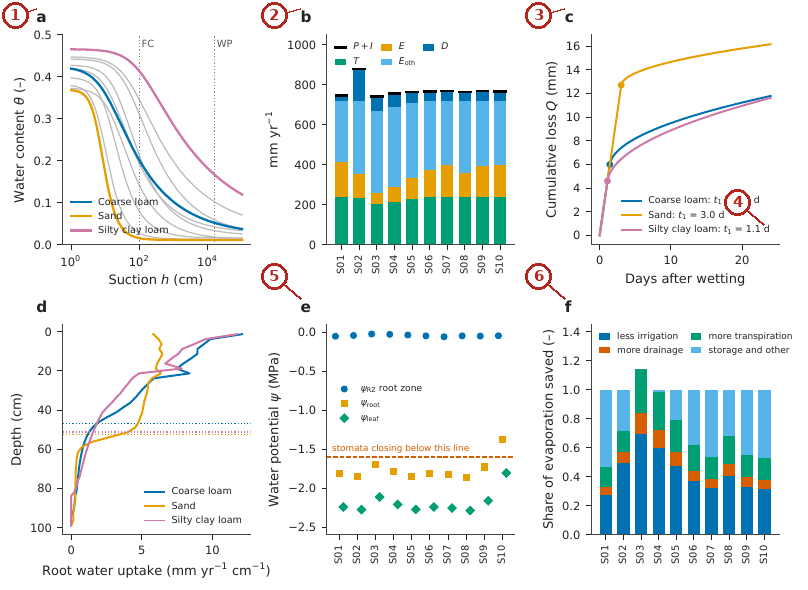
\includegraphics[width=\textwidth,height=0.42\textheight,keepaspectratio]{../figures/annot/p2_fig-swa_0.png}\end{center}

\textbf{What the numbered labels point to.}
\begin{enumerate}[nosep,label=\protect\circled{\arabic*}]
\item Panel (a): see the caption above. \emph{Why:} Sands release their water at low suction, clays over a wide range, so the curves cross field capacity and wilting point at different contents.
\item Panel (b): Annual balance: sinks stacked ($T$, $E$, $E_{\mathrm{oth}}$, $D$) against the input $P+I$ (black marks). \emph{Why:} The same rain leaves as drainage in coarse soils and as evaporation and transpiration in fine soils.
\item Panel (c): Cumulative evaporation after a wetting at the season-mean demand (Eq.~(11) of the article); dots mark the end of stage 1. \emph{Why:} Fine soils keep the surface wet longer, so stage 1 lasts longer.
\item Panel (d): Mean annual root water uptake by depth from Engine~2 (unscaled); dotted lines mark $z_{90}$. \emph{Why:} Uptake follows root density, which falls with depth.
\item Panel (e): Water potential of the root zone, the root surface and the leaf (Eq.~(21) and Eq.~(22) of the article), crop days of day-of-year 120--210; the dashed line is the stomatal-closure threshold of the view; the air is at $-56$\,MPa (not shown). \emph{Why:} Potential falls from root zone to leaf because water flows through resistances; dry soil adds a large soil resistance.
\item Panel (f): Fate of the soil evaporation saved by a straw mulch (Eq.~(23) of the article); in sand the three positive shares sum to 1.14, so the remainder is zero. \emph{Why:} A mulch saving goes to transpiration, less irrigation or drainage according to the soil.
\end{enumerate}

\textbf{What it shows.} Soil--water--atmosphere variables of the ten soils at the reference state. (a) Retention curves $\theta(h)$ (Eq.~(27) and Eq.~(2) of the article); sand, coarse loam and silty clay loam highlighted; dotted lines are field capacity (FC, 100\,cm) and the wilting point (WP, 15\,849\,cm). (b) Annual balance: sinks stacked ($T$, $E$, $E_{\mathrm{oth}}$, $D$) against the input $P+I$ (black marks). (c) Cumulative evaporation after a wetting at the season-mean demand (Eq.~(11) of the article); dots mark the end of stage 1. (d) Mean annual root water uptake by depth from Engine~2 (unscaled); dotted lines mark $z_{90}$. (e) Water potential of the root zone, the root surface and the leaf (Eq.~(21) and Eq.~(22) of the article), crop days of day-of-year 120--210; the dashed line is the stomatal-closure threshold of the view; the air is at $-56$\,MPa (not shown). (f) Fate of the soil evaporation saved by a straw mulch (Eq.~(23) of the article); in sand the three positive shares sum to 1.14, so the remainder is zero.

\textbf{How to read the labels, symbols and colours.} (a) Retention curves with field capacity and wilting point dotted; (b) annual sinks stacked against the input (black marks); (c) cumulative evaporation after wetting, dots at the end of stage 1; (d) root uptake by depth; (e) water potential of root zone, root surface and leaf; (f) fate of a mulch saving.

\textbf{What affects it, and why it happens.} Soils differ in how much water they hold between field capacity and wilting point and how fast they pass it on; these differences propagate to evaporation, uptake, potential and the fate of a saving.

\textbf{How it is made.} Figure drawn by the script from the input data. Script: \nolinkurl{Manuscripts/reproducibility/analysis/p3_swa_fig.py}. Input: \nolinkurl{Data/daisy_ensemble.csv.gz}.


\subsection{Reading Figure 4 of the article}
\begin{center}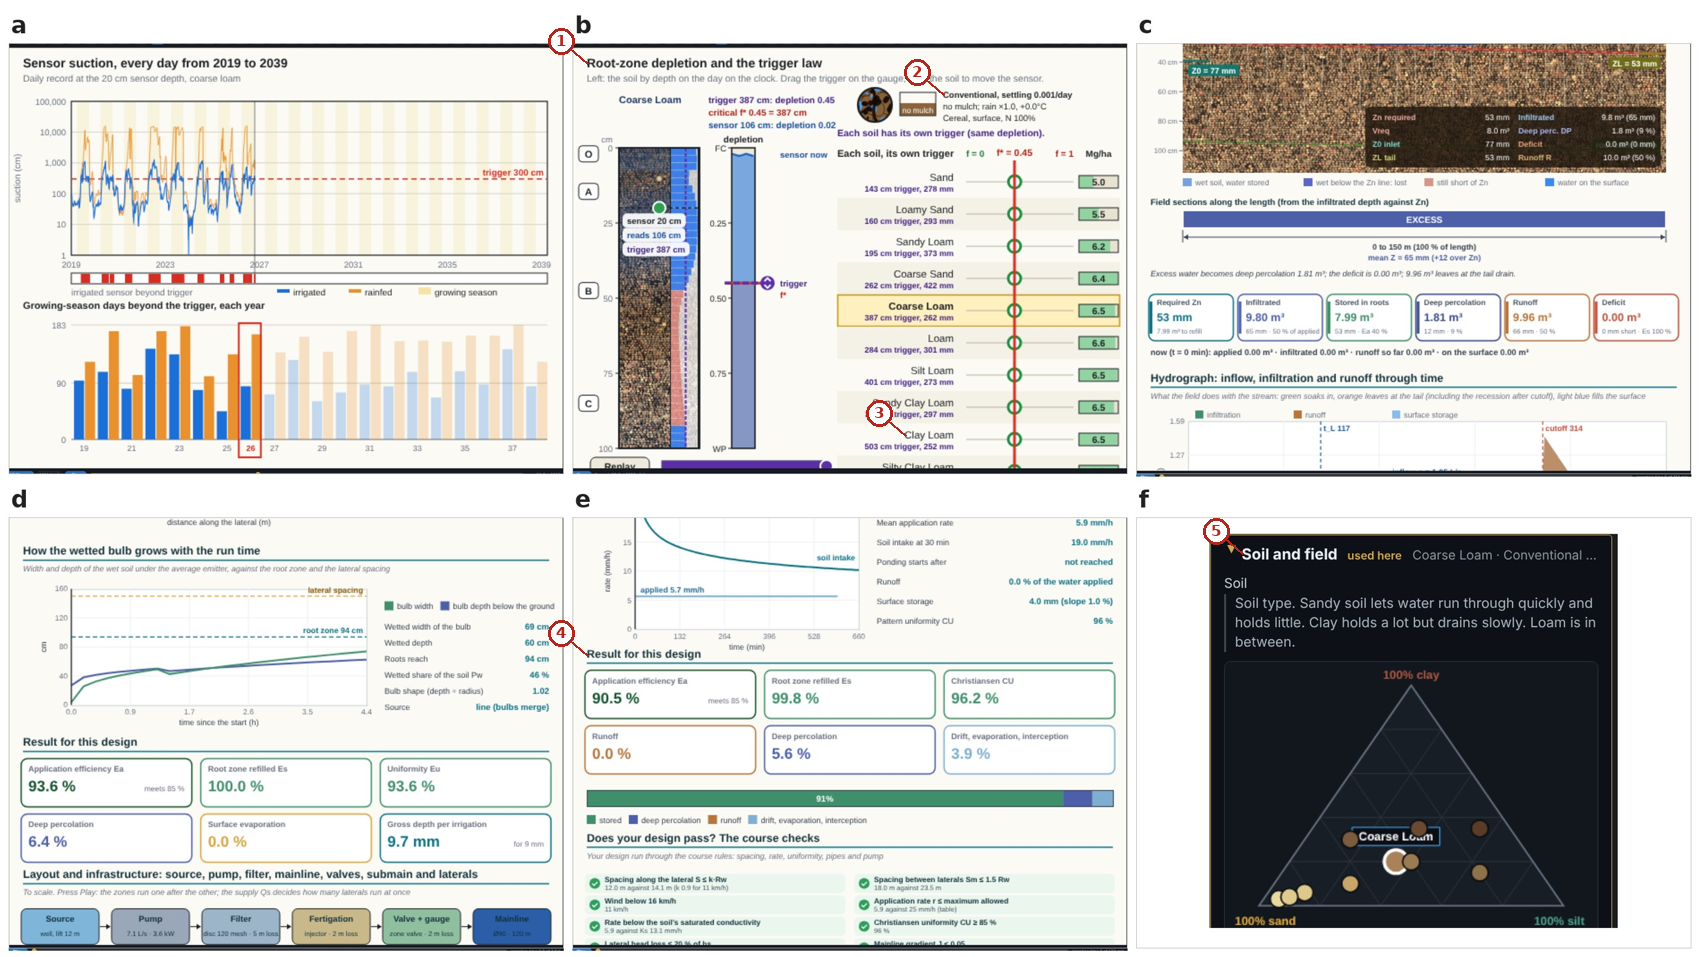
\includegraphics[width=\textwidth,height=0.42\textheight,keepaspectratio]{../figures/annot/p2_fig-viewsB_0.png}\end{center}

\textbf{What the numbered labels point to.}
\begin{enumerate}[nosep,label=\protect\circled{\arabic*}]
\item ``Root-zone depletion and the trigger law'': the suction (or depletion) at which irrigation starts.
\item ``Conventional'': a heading or control of this screen; the caption above says which layer it belongs to.
\item ``Clay Loam'': the soil of the project, which every layer uses.
\item ``Result for this design'': a heading or control of this screen; the caption above says which layer it belongs to.
\item ``Soil and field'': the soil of the project, which every layer uses.
\end{enumerate}

\textbf{What it shows.} Result views for irrigation timing and design. (a) Sensor and trigger; (b) irrigation rule collapsing ten soils onto one depletion curve; (c) surface irrigation; (d) drip irrigation; (e) sprinklers; (f) soil selection on the texture triangle, which drives every view.

\textbf{How to read the labels, symbols and colours.} Views for timing and design (sensor and trigger, the trigger rule, surface, drip, sprinkler, soil triangle).

\textbf{What affects it, and why it happens.} Expressing the trigger as depletion collapses the soils onto one curve; the designs follow the soil intake and the water needed. The trigger rule collapses the soils onto one depletion curve because it uses depletion, not suction; the designs follow from the soil's intake and the water needed.

\textbf{How it is made.} Screen capture of SWAFL Desktop 1.1.0 (not regenerated).


\subsection{Reading Figure 14 of the article}
\begin{center}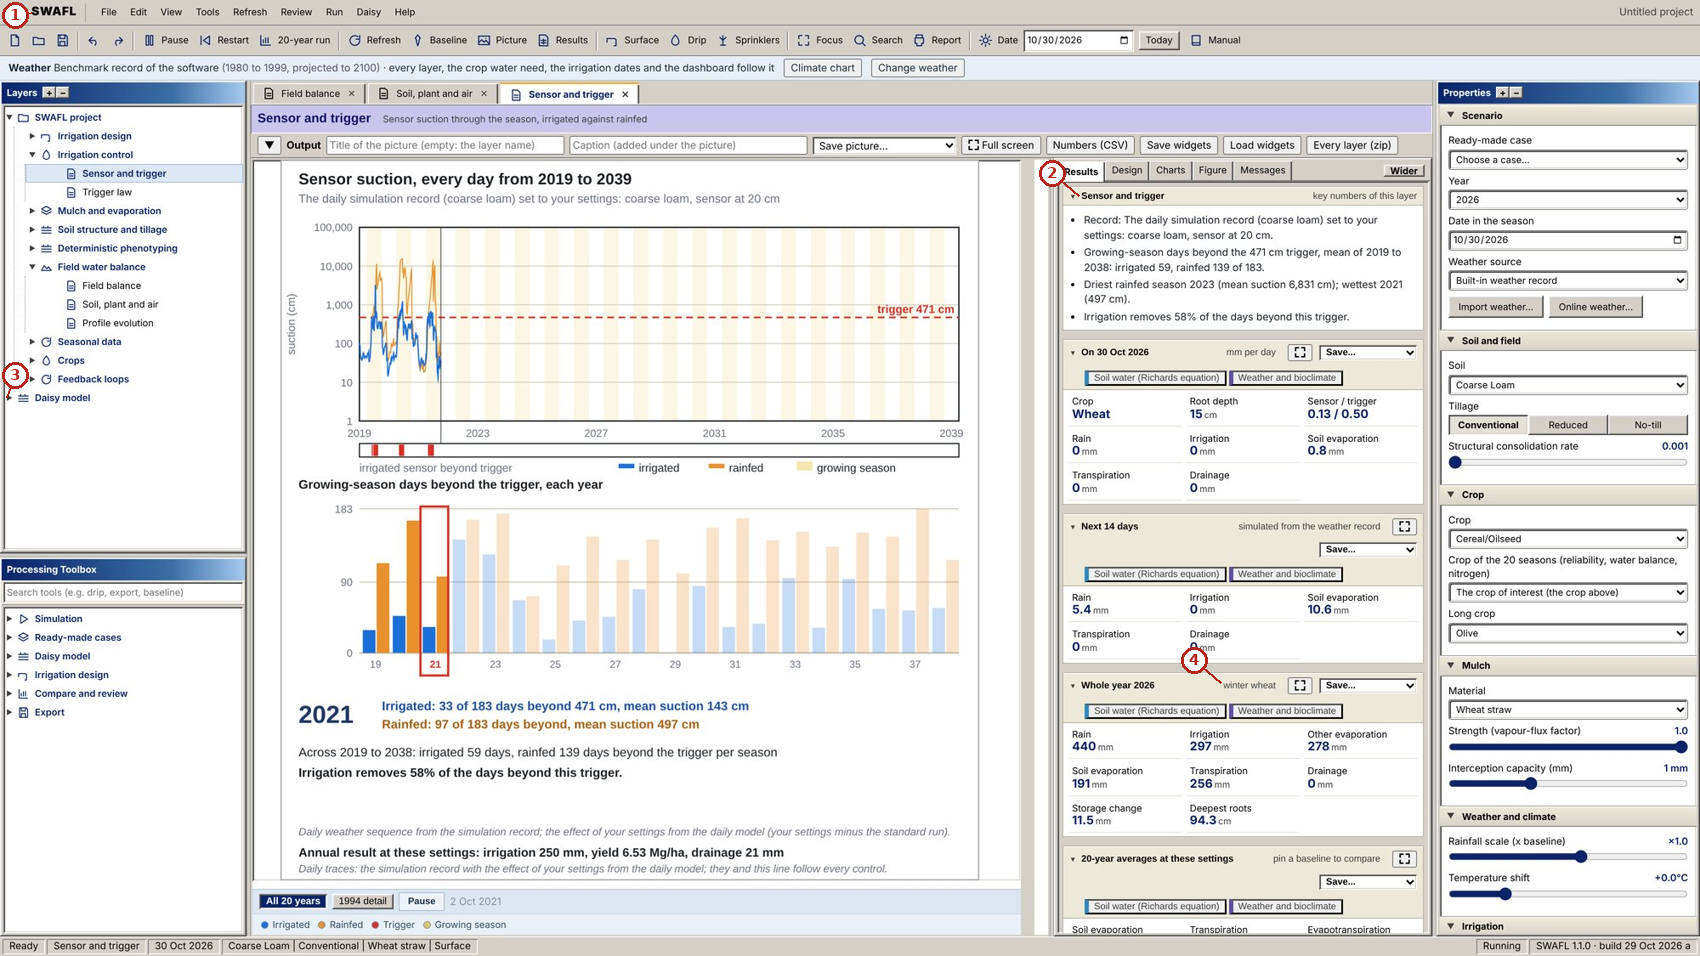
\includegraphics[width=\textwidth,height=0.42\textheight,keepaspectratio]{../figures/annot/p2_fig-shot-layer-v1_0.png}\end{center}

\textbf{What the numbered labels point to (picture 1 of 2: Sensor and trigger: 20 years of daily suction at the sensor, irrigated and rainfed, against the trigger, and the days beyond the trigger per year (Eq.~(8) of the article).).}
\begin{enumerate}[nosep,label=\protect\circled{\arabic*}]
\item ``SWAFL View Run Daisy Help'': the menu bar of the program (file, view, run, Daisy, help).
\item ``Sensor and trigger'': the suction (or depletion) at which irrigation starts.
\item ``Daisy model'': the Daisy model and its workbench.
\item ``winter'': a heading or control of this screen; the caption above says which layer it belongs to.
\end{enumerate}

\begin{center}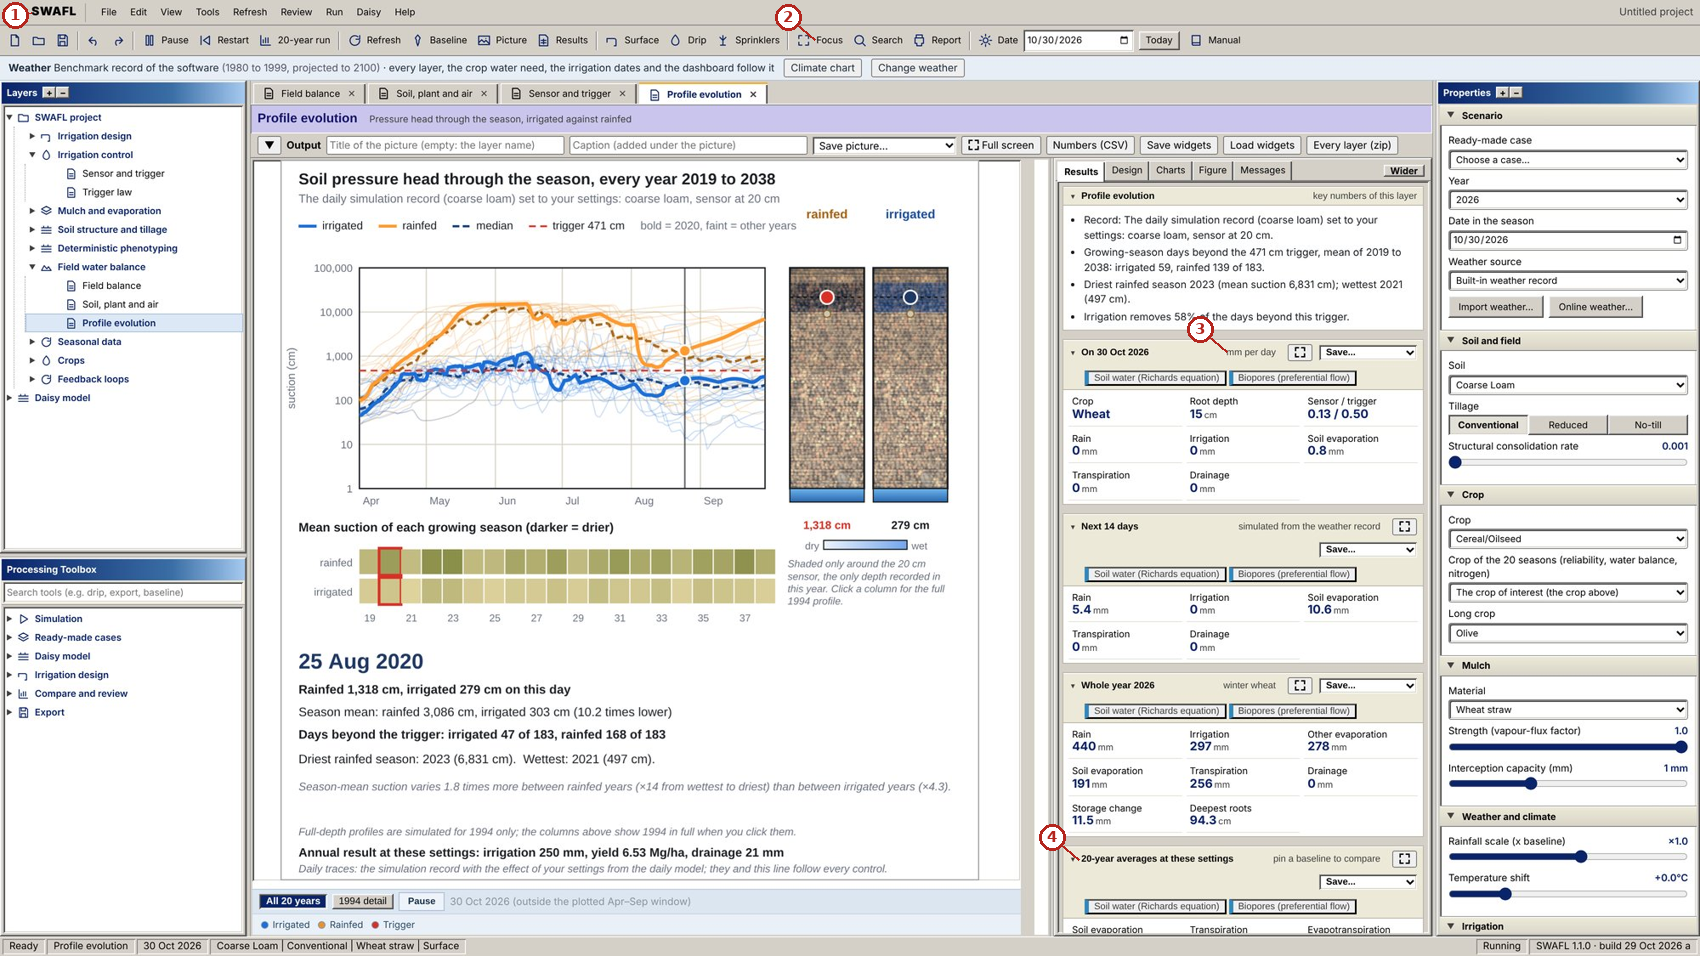
\includegraphics[width=\textwidth,height=0.42\textheight,keepaspectratio]{../figures/annot/p2_fig-shot-layer-v1_1.png}\end{center}

\textbf{What the numbered labels point to (picture 2 of 2: Profile evolution: pressure-head profile through the season, irrigated and rainfed, and the share of the root zone beyond the trigger (Eq.~(9) of the article).).}
\begin{enumerate}[nosep,label=\protect\circled{\arabic*}]
\item ``SWAFL View Run Daisy Help'': the menu bar of the program (file, view, run, Daisy, help).
\item ``Focus Q Search'': a heading or control of this screen; the caption above says which layer it belongs to.
\item ``mm per day'': a rate in millimetres per day.
\item ``20-year averages at these settings'': a heading or control of this screen; the caption above says which layer it belongs to.
\end{enumerate}

\textbf{What it shows.} SWAFL Desktop: soil water and irrigation timing. Panels: (a) Sensor and trigger: 20 years of daily suction at the sensor, irrigated and rainfed, against the trigger, and the days beyond the trigger per year (Eq.~(8) of the article). (b) Profile evolution: pressure-head profile through the season, irrigated and rainfed, and the share of the root zone beyond the trigger (Eq.~(9) of the article).

\textbf{How to read the labels, symbols and colours.} A screen of the software as it appears to the user; the labelled areas are the inputs, the figure and the numbers of the layer named in the caption.

\textbf{What affects it, and why it happens.} The suction at the sensor rises as the crop dries the soil and falls after each rain or irrigation; irrigation is triggered when it crosses the trigger line. 

\textbf{How it is made.} Screen capture of SWAFL Desktop 1.1.0 (not regenerated).


\subsection{Reading Figure 15 of the article}
\begin{center}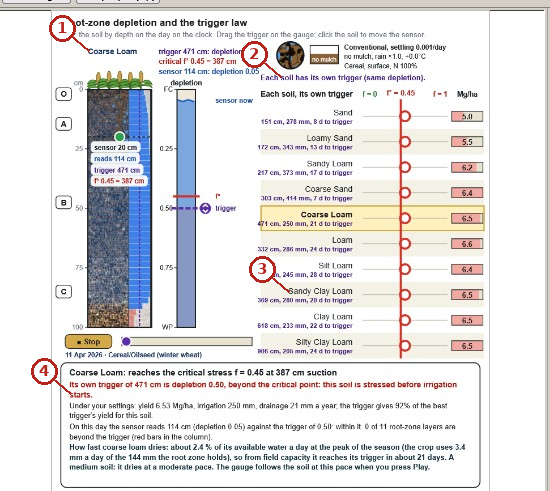
\includegraphics[width=\textwidth,height=0.42\textheight,keepaspectratio]{../figures/annot/p2_fig-shot-layer-n1_0.png}\end{center}

\textbf{What the numbered labels point to.}
\begin{enumerate}[nosep,label=\protect\circled{\arabic*}]
\item ``Coarse Loam'': the soil of the project, which every layer uses.
\item ``soil has Its own trigger'': the suction (or depletion) at which irrigation starts.
\item ``Sandy'': the soil of the project, which every layer uses.
\item ``starts'': a heading or control of this screen; the caption above says which layer it belongs to.
\end{enumerate}

\textbf{What it shows.} SWAFL Desktop: trigger law. Panels: (a) Trigger law: root-zone depletion of ten soils on one axis with the critical depletion $f^\ast$, each soil's own trigger suction and yield, and the gauge of the sensor through the season (Eq.~(29) and Eq.~(25) and Eq.~(26) of the article).

\textbf{How to read the labels, symbols and colours.} A screen of the software as it appears to the user; the labelled areas are the inputs, the figure and the numbers of the layer named in the caption.

\textbf{What affects it, and why it happens.} Each soil reaches the same depletion at a different suction because of the shape of its retention curve, so each soil has its own trigger. 

\textbf{How it is made.} Screen capture of SWAFL Desktop 1.1.0 (not regenerated).


\subsection{Reading Figure 30 of the article}
\begin{center}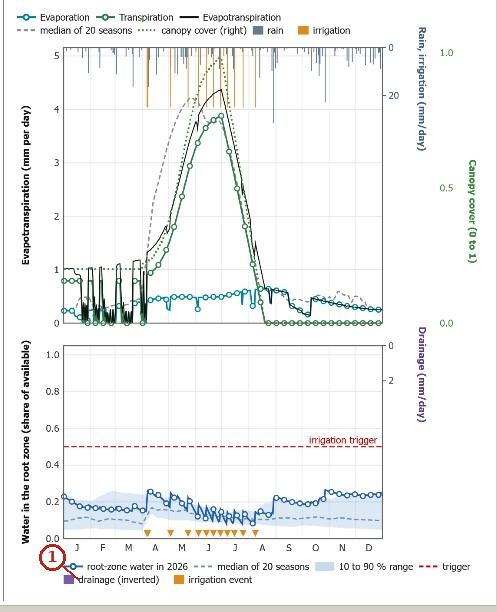
\includegraphics[width=\textwidth,height=0.42\textheight,keepaspectratio]{../figures/annot/p2_fig-shot-real-balance_0.png}\end{center}

\textbf{What the numbered labels point to (picture 1 of 2: Field balance, charts: evaporation, transpiration and evapotranspiration of 2026 against the median of 20 seasons, with rain, irrigation and canopy cover, and the root-zone water against the trigger with the 10 to 90\,\% range and the irrigation events.).}
\begin{enumerate}[nosep,label=\protect\circled{\arabic*}]
\item ``drainage (inverted) event'': rain, from the weather of the project.
\end{enumerate}

\begin{center}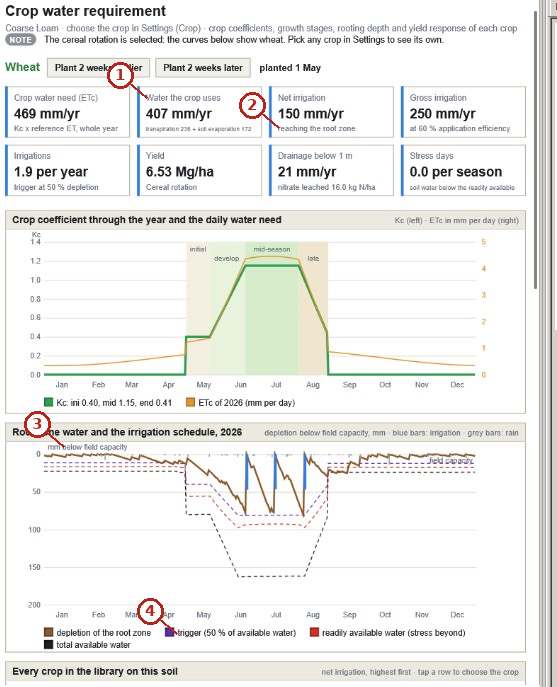
\includegraphics[width=\textwidth,height=0.42\textheight,keepaspectratio]{../figures/annot/p2_fig-shot-real-balance_1.png}\end{center}

\textbf{What the numbered labels point to (picture 2 of 2: Crop water requirement: crop coefficient and daily need through the year, and the root-zone depletion with the trigger, the readily and the totally available water and the irrigations of 2026.).}
\begin{enumerate}[nosep,label=\protect\circled{\arabic*}]
\item ``Water the crop uses'': the crop of the project and its stage.
\item ``reaching the root zone'': the roots: depth, density and uptake.
\item ``below capacity'': a heading or control of this screen; the caption above says which layer it belongs to.
\item ``trigger (50 \% of available water)'': the suction (or depletion) at which irrigation starts.
\end{enumerate}

\textbf{What it shows.} SWAFL Desktop: the field water balance and the crop water requirement through the year (screen captures of release 1.1.0). Panels: (a) Field balance, charts: evaporation, transpiration and evapotranspiration of 2026 against the median of 20 seasons, with rain, irrigation and canopy cover, and the root-zone water against the trigger with the 10 to 90\,\% range and the irrigation events. (b) Crop water requirement: crop coefficient and daily need through the year, and the root-zone depletion with the trigger, the readily and the totally available water and the irrigations of 2026.

\textbf{How to read the labels, symbols and colours.} A screen of the software as it appears to the user; the labelled areas are the inputs, the figure and the numbers of the layer named in the caption.

\textbf{What affects it, and why it happens.} Evapotranspiration follows the crop coefficient through the season; root-zone water falls between irrigations and is refilled at the trigger. 

\textbf{How it is made.} Screen capture of SWAFL Desktop 1.1.0 (not regenerated).


\subsection{Reading Figure 6 of the article}
\begin{center}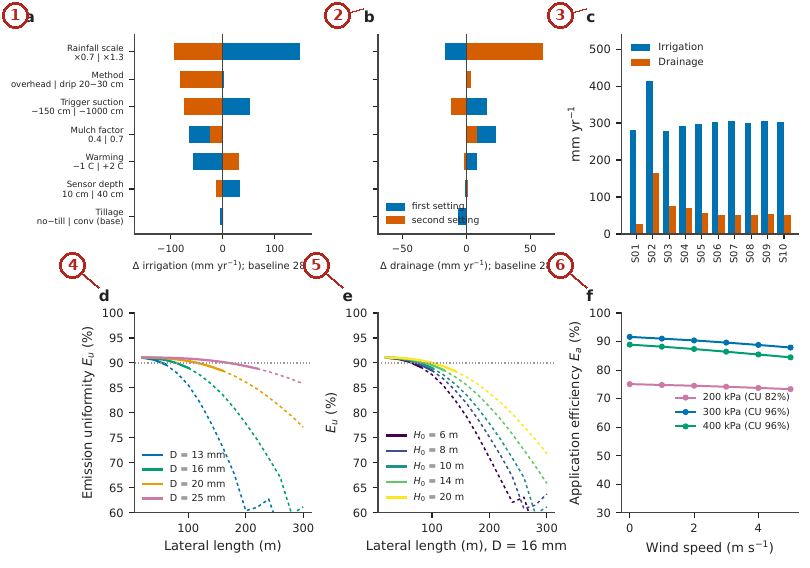
\includegraphics[width=\textwidth,height=0.42\textheight,keepaspectratio]{../figures/annot/p2_fig-sens_0.png}\end{center}

\textbf{What the numbered labels point to.}
\begin{enumerate}[nosep,label=\protect\circled{\arabic*}]
\item Panel (a): Engine~1 annual irrigation and. \emph{Why:} Controls that raise demand or lower supply raise irrigation.
\item Panel (b): drainage change for each control moved to the two settings listed under its name (blue: first setting; orange: second setting) from the reference state; nitrogen rate, which leaves both unchanged, is not shown. \emph{Why:} Controls that keep the profile wet raise drainage.
\item Panel (c): Irrigation and drainage by soil. \emph{Why:} Coarse soils need more irrigation and drain more.
\item Panel (d): Drip emission uniformity against lateral length by lateral diameter and. \emph{Why:} Longer laterals carry more flow over more length, so friction lowers the head at the end and uniformity falls.
\item Panel (e): by inlet head; dashed where $h_f/H_0>0.2$. \emph{Why:} A higher inlet head makes friction a smaller share of the head, so uniformity rises.
\item Panel (f): Sprinkler application efficiency against wind speed at 200, 300 and 400\,kPa (CU in the legend). \emph{Why:} Wind distorts and blows away part of the spray, so efficiency falls; higher pressure makes smaller drops that drift more.
\end{enumerate}

\textbf{What it shows.} One-at-a-time sensitivity of SWAFL Desktop outputs. (a) Engine~1 annual irrigation and (b) drainage change for each control moved to the two settings listed under its name (blue: first setting; orange: second setting) from the reference state; nitrogen rate, which leaves both unchanged, is not shown. (c) Irrigation and drainage by soil. (d) Drip emission uniformity against lateral length by lateral diameter and (e) by inlet head; dashed where $h_f/H_0>0.2$. (f) Sprinkler application efficiency against wind speed at 200, 300 and 400\,kPa (CU in the legend).

\textbf{How to read the labels, symbols and colours.} (a, b) Change of irrigation and drainage when each control moves to two settings (blue, orange); (c) by soil; (d, e) drip uniformity against lateral length, diameter and inlet head; (f) sprinkler efficiency against wind.

\textbf{What affects it, and why it happens.} Controls that change water supply or demand move irrigation and drainage most; long or narrow laterals lose head and uniformity; wind distorts the sprinkler pattern.

\textbf{How it is made.} Figure drawn by the script from the input data. Script: \nolinkurl{Manuscripts/reproducibility/analysis/p3_sens_fig.py}. Input: \nolinkurl{Data/daisy_ensemble.csv.gz}.


\subsection{Derivation: Capillary radius}\label{der:s2:2}
The pressure jump across a meniscus in a cylindrical pore of radius $r$ is $\Delta p=2\sigma\cos\gamma_c/r$ (Young--Laplace). Equating with the suction head $\rho_wgh$ gives $r_c=2\sigma\cos\gamma_c/(\rho_wgh)$; with $\sigma=0.0728$\,N\,m$^{-1}$, $\gamma_c=0$, $\rho_w=1000$\,kg\,m$^{-3}$ and $g=9.81$\,m\,s$^{-2}$, $r_c=1.49\times10^{-5}\,\mathrm{m^2}/h=0.149\,\mathrm{cm^2}/h$: the pores emptied at a suction $h$ are those wider than $r_c$.


\subsection{Derivation: Depletion and the trigger law}\label{der:s2:3}
The plant-available water lies between field capacity (100\,cm) and the wilting point (15\,849\,cm). The depletion at suction $h$ is the share of that water that has been used, $f(h)=[S_e(100)-S_e(h)]/[S_e(100)-S_e(15\,849)]$, because $\theta-\theta_r$ is proportional to $S_e$ and the factor $\theta_s-\theta_r$ cancels. The suction that corresponds to a chosen depletion $f^\ast$ is found by inverting: $S_e(h^\ast)=S_e(100)-f^\ast[S_e(100)-S_e(15\,849)]$ and $h^\ast=\alpha^{-1}(S_e^{-1/m}-1)^{1/n}$. A soil-independent depletion therefore gives a soil-specific suction, which is why one suction trigger uses different shares of the available water in different soils.


\subsection{Why it happens}
\paragraph{Why the same trigger uses different shares of the available water.} A suction trigger marks a point on the retention curve. In a sand most available water is released at low suctions, so a $-300$\,cm trigger is reached late (much of the water used); in a clay the water is released over a wide range, so the same suction is reached early.

\paragraph{Why the daily model fails in sand at dry triggers.} In sand dry triggers lie beyond the suction the crop can produce in the soil, so the full simulation seldom irrigates, while the daily bucket, which has no conductivity limit, still reaches the trigger.


\section{Rainfall and interception}
The interception store of the daily model and the drainage that follows rain.

\subsection{Contribution 2: an interception store that matches the annual model}\label{con:s2:2}
\begin{problem}
The daily model must lose to canopy interception the same water per year as the annual model, although its rain falls in random daily amounts. How large must the daily interception store be?
\end{problem}
\begin{derivation}
Daily rain was taken as exponential with mean $\mu_0$; the throughfall above a store $I_c$ was integrated over that distribution; the result was set equal to the throughfall fraction of the annual model and solved for $I_c$.
\end{derivation}
\begin{keyresult}
\begin{pencil}
{\small\noindent\textbf{How it is derived, line by line}
\[\begin{array}{@{}l@{}}\textbf{1. Daily rain exponential:}\\[1pt]
\qquad p(R)=\mu_0^{-1}e^{-R/\mu_0}\\[1pt]
\textbf{2. Expected throughfall above } I_c\textbf{:}\\[1pt]
\qquad \textstyle\int_{I_c}^\infty(R-I_c)p(R)\,\dd R=\mu_0e^{-I_c/\mu_0}\\[1pt]
\textbf{3. Throughfall fraction:}\\[1pt]
\qquad r=e^{-I_c/\mu_0}\\[1pt]
\textbf{4. Solve for } I_c\textbf{:}\\[1pt]
\qquad I_c=\mu_0\ln(1/r)
\end{array}\]}
\noindent\textbf{The result, with its parts marked}
\[\underbrace{\mathrm E[(R-I_c)^+]}_{\circled{1}}=\mu_0e^{-I_c/\mu_0}\;\Rightarrow\;\underbrace{r=e^{-I_c/\mu_0}}_{\circled{2}}\;\Rightarrow\;\underbrace{I_c=\mu_0\ln\frac1r}_{\circled{3}}\]
\end{pencil}
\end{keyresult}
\begin{pins}
\pin{1}{Expected throughfall of an exponential daily rain of mean $\mu_0$ above a store $I_c$, obtained by integrating the exponential density.}
\pin{2}{The throughfall fraction; it is set equal to the throughfall of the annual model.}
\pin{3}{The store follows in closed form: with $\mu_0=4.5$\,mm and $r=0.9$, $I_c=0.47$\,mm. The two engines therefore agree on interception by construction.}
\end{pins}


\subsection{Worked numbers, part 3: interception by the canopy}
If daily rain is exponential with mean $\mu_0$, a store $I_c$ lets through the fraction $r=e^{-I_c/\mu_0}$, so $I_c=\mu_0\ln(1/r)$. \emph{Example:} $\mu_0=4.5$\,mm and $r=0.9$ give $I_c=4.5\times0.105=0.47$\,mm.


\subsection{Reading Figure 9 of the article}
\begin{center}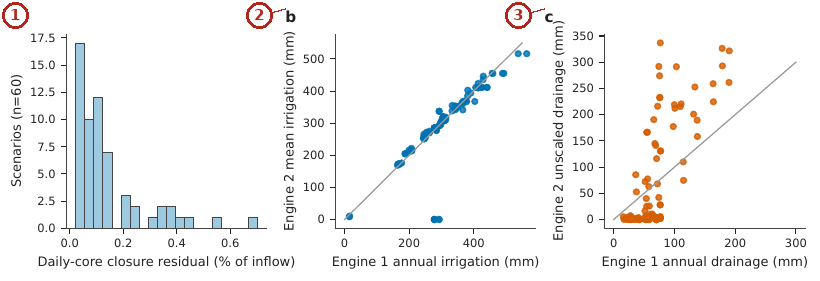
\includegraphics[width=\textwidth,height=0.42\textheight,keepaspectratio]{../figures/annot/p2_fig-e2_0.png}\end{center}

\textbf{What the numbered labels point to.}
\begin{enumerate}[nosep,label=\protect\circled{\arabic*}]
\item Panel (a): Closure residual of the unscaled daily core over 60 random states. \emph{Why:} The daily model conserves water by construction, so the residual is near zero.
\item Panel (b): Mean annual irrigation of Engine 2 against Engine 1 for the 100 scenarios of the realistic grid (10 soils $\times$ 5 triggers $\times$ 2 methods, cereal), including the failures at zero. \emph{Why:} Irrigation of the two engines agrees except in sand at dry triggers, where the daily bucket reaches triggers that the full model cannot.
\item Panel (c): Unscaled Engine 2 drainage against Engine 1 for the same scenarios. \emph{Why:} Drainage agrees in order but the bucket drains in steps, so levels differ.
\end{enumerate}

\textbf{What it shows.} Engine 2. (a) Closure residual of the unscaled daily core over 60 random states. (b) Mean annual irrigation of Engine 2 against Engine 1 for the 100 scenarios of the realistic grid (10 soils $\times$ 5 triggers $\times$ 2 methods, cereal), including the failures at zero. (c) Unscaled Engine 2 drainage against Engine 1 for the same scenarios.

\textbf{How to read the labels, symbols and colours.} (a) Closure residual over 60 states; (b) irrigation and (c) drainage of Engine 2 against Engine 1 for 100 scenarios.

\textbf{What affects it, and why it happens.} The residual is near zero because the daily model conserves water by construction; agreement with Engine 1 fails in sand at dry triggers where the daily bucket reaches triggers the full model cannot.

\textbf{How it is made.} Figure drawn by the script from the input data. Script: \nolinkurl{Manuscripts/reproducibility/analysis/p3_figs.py}. Input: \nolinkurl{Data/daisy_ensemble.csv.gz}.


\subsection{Reading Figure 16 of the article}
\begin{center}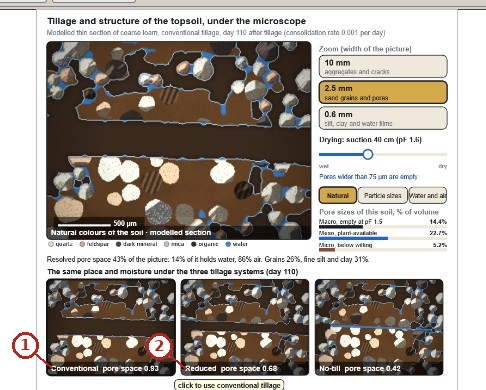
\includegraphics[width=\textwidth,height=0.42\textheight,keepaspectratio]{../figures/annot/p2_fig-shot-layer-v3_0.png}\end{center}

\textbf{What the numbered labels point to (picture 1 of 2: Tillage and structure: modelled thin section of the topsoil with the water- and air-filled pores at the chosen suction, the pore sizes, and the same place under conventional, reduced and no tillage (Eq.~(3) of the article)).}
\begin{enumerate}[nosep,label=\protect\circled{\arabic*}]
\item ``Conventional'': a heading or control of this screen; the caption above says which layer it belongs to.
\item ``Reduced pore 0.68'': a heading or control of this screen; the caption above says which layer it belongs to.
\end{enumerate}

\begin{center}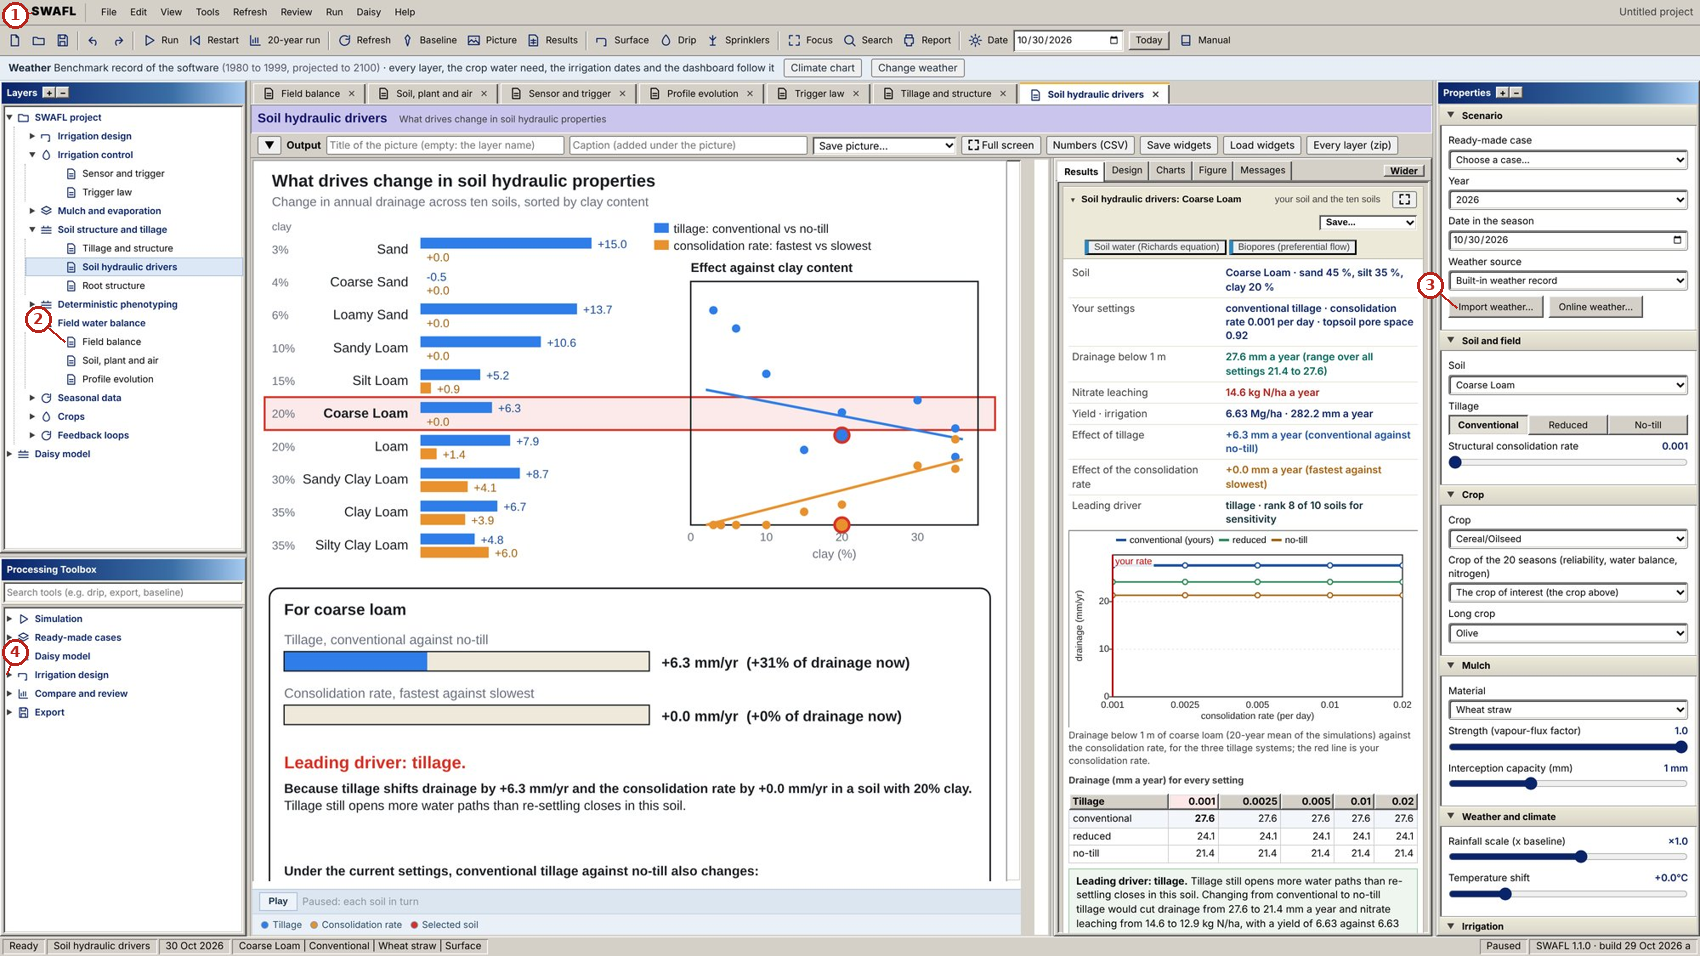
\includegraphics[width=\textwidth,height=0.42\textheight,keepaspectratio]{../figures/annot/p2_fig-shot-layer-v3_1.png}\end{center}

\textbf{What the numbered labels point to (picture 2 of 2: Soil hydraulic drivers: tillage and consolidation effects on drainage for the ten soils and their regressions on clay content (Eq.~(5) of the article).).}
\begin{enumerate}[nosep,label=\protect\circled{\arabic*}]
\item ``SWAFL View Run Daisy Help'': the menu bar of the program (file, view, run, Daisy, help).
\item ``Field balance'': the field water balance: inputs, outputs and storage of the root zone.
\item ``Import weather... Online weather'': the weather of the project: built-in record, a file of the user or online weather of any place.
\item ``design'': a heading or control of this screen; the caption above says which layer it belongs to.
\end{enumerate}

\textbf{What it shows.} SWAFL Desktop: soil structure and hydraulic drivers. Panels: (a) Tillage and structure: modelled thin section of the topsoil with the water- and air-filled pores at the chosen suction, the pore sizes, and the same place under conventional, reduced and no tillage (Eq.~(3) of the article). (b) Soil hydraulic drivers: tillage and consolidation effects on drainage for the ten soils and their regressions on clay content (Eq.~(5) of the article).

\textbf{How to read the labels, symbols and colours.} A screen of the software as it appears to the user; the labelled areas are the inputs, the figure and the numbers of the layer named in the caption.

\textbf{What affects it, and why it happens.} Tillage opens large pores that hold little water and drain fast; consolidation closes them over time, which changes drainage. 

\textbf{How it is made.} Screen capture of SWAFL Desktop 1.1.0 (not regenerated).


\subsection{Reading Figure 17 of the article}
\begin{center}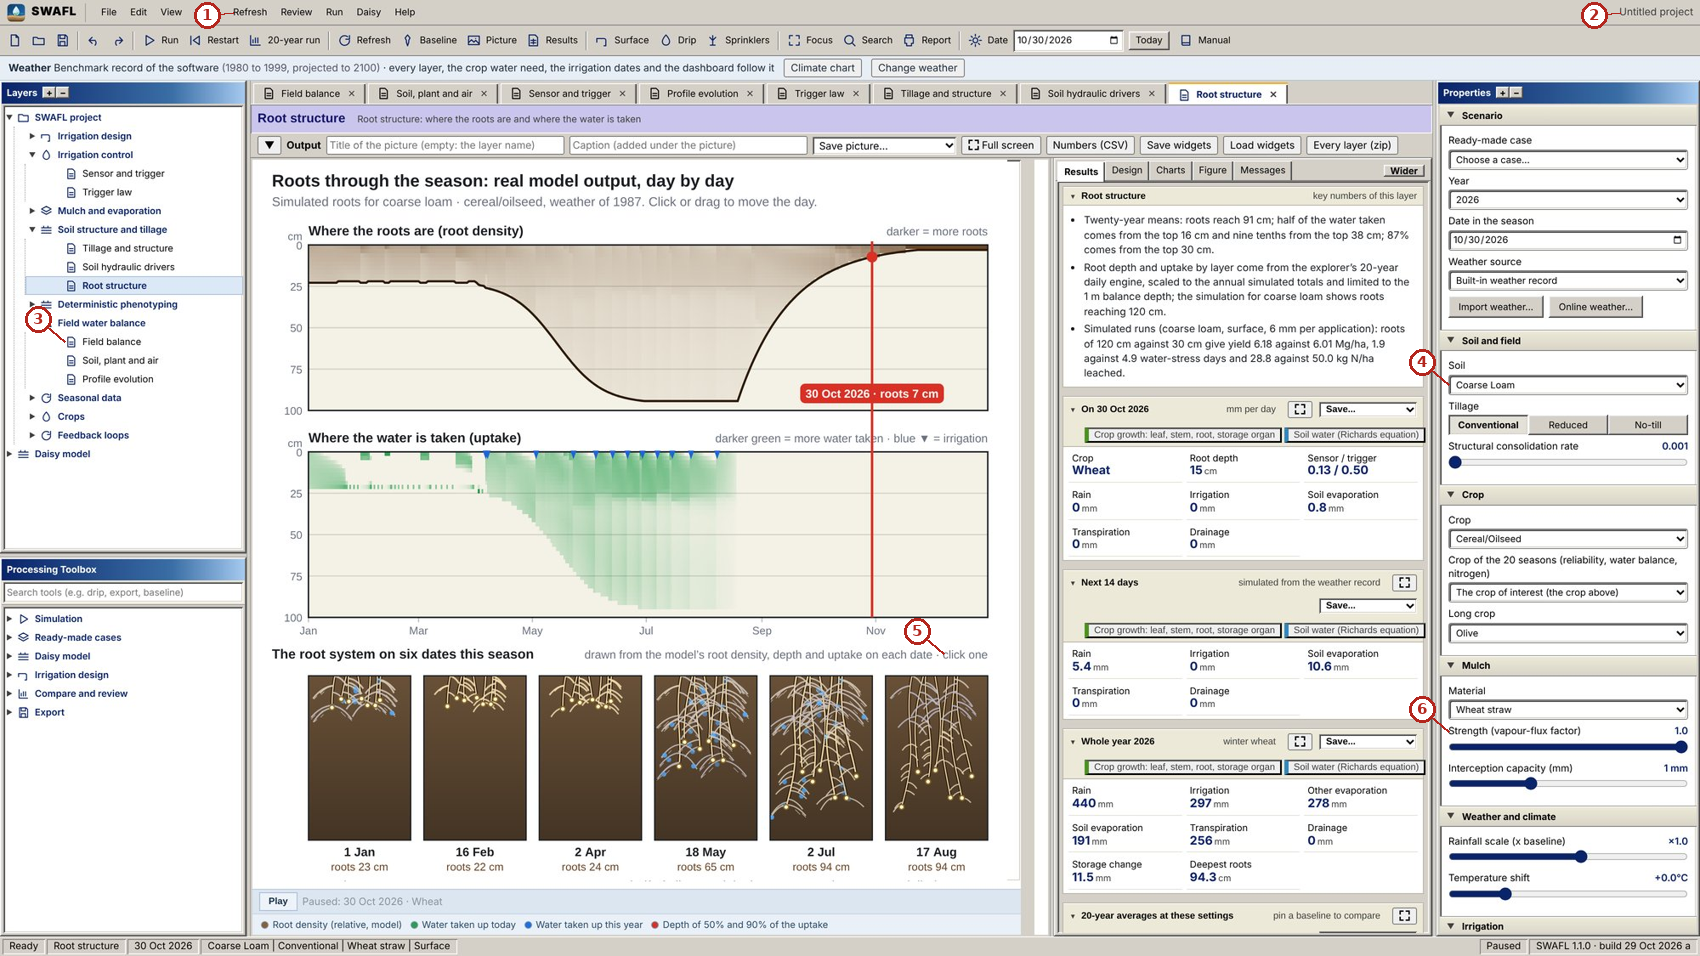
\includegraphics[width=\textwidth,height=0.42\textheight,keepaspectratio]{../figures/annot/p2_fig-shot-layer-r1_0.png}\end{center}

\textbf{What the numbered labels point to.}
\begin{enumerate}[nosep,label=\protect\circled{\arabic*}]
\item ``Refresh Review Run Help'': a heading or control of this screen; the caption above says which layer it belongs to.
\item ``Untitled project'': a heading or control of this screen; the caption above says which layer it belongs to.
\item ``Field balance'': the field water balance: inputs, outputs and storage of the root zone.
\item ``Coarse Loam v'': the soil of the project, which every layer uses.
\item ``click one'': a heading or control of this screen; the caption above says which layer it belongs to.
\item ``Strength (vapour-flux factor)'': a heading or control of this screen; the caption above says which layer it belongs to.
\end{enumerate}

\textbf{What it shows.} SWAFL Desktop: roots. Panels: (a) Root structure: rooting depth and the depths holding 50 and 90\,\% of uptake in the ten soils (Eq.~(17) and Eq.~(18) and Eq.~(19) and Eq.~(20) of the article), with the E15 rooting-depth heat maps.

\textbf{How to read the labels, symbols and colours.} A screen of the software as it appears to the user; the labelled areas are the inputs, the figure and the numbers of the layer named in the caption.

\textbf{What affects it, and why it happens.} Roots go deeper in soils that let them and where water is deeper; uptake follows root density. 

\textbf{How it is made.} Screen capture of SWAFL Desktop 1.1.0 (not regenerated).


\subsection{Derivation: Rainfall and interception of the daily model}\label{der:s2:8}
If daily rain depths are exponential with mean $\mu_0$, the expected throughfall above an interception store $I_c$ is $\mathrm E[(R-I_c)^+]=\int_{I_c}^\infty(R-I_c)\mu_0^{-1}e^{-R/\mu_0}\dd R=\mu_0e^{-I_c/\mu_0}$. The throughfall fraction is $r=e^{-I_c/\mu_0}$, hence $I_c=\mu_0\ln(1/r)$: the store is chosen so that the expected interception equals the annual interception of the annual model.


\subsection{Why it happens}
\paragraph{Why drainage differs under the same rain.} Drainage is the water that exceeds what the profile holds and the crop uses; profiles that hold less (sands) and conduct more pass more water below 1\,m.

\section{Evaporation and the soil--plant--atmosphere path}
The two stages of soil evaporation and the water potential from the soil to the air.

\subsection{Contribution 3: two evaporation stages joined without a jump}\label{con:s2:3}
\begin{derivation}
Stage 1 runs at the demand $e_0$ until the stage-1 limit $Q_1$; for stage 2 a square-root law of diffusion was taken, and its two constants were set so that the rate equals $e_0$ at the change of stage and the long-time behaviour is $\sqrt t$.
\end{derivation}
\begin{keyresult}
\begin{pencil}
{\small\noindent\textbf{How it is derived, line by line}
\[\begin{array}{@{}l@{}}\textbf{1. Stage 1 at demand:}\\[1pt]
\qquad Q=q_0+e_0t,\ t\le t_1\\[1pt]
\textbf{2. Stage 2, square-root form:}\\[1pt]
\qquad Q=Q_1+A(\sqrt{1+(t-t_1)/\tau_E}-1)\\[1pt]
\textbf{3. Rate continuous at } t_1\textbf{:}\\[1pt]
\qquad \dd Q/\dd t|_{t_1}=A/(2\tau_E)=e_0\Rightarrow A=2e_0\tau_E
\end{array}\]}
\noindent\textbf{The result, with its parts marked}
\[Q(t)=Q_1+\underbrace{2e_0\tau_E}_{\circled{1}}\Bigl(\sqrt{1+\underbrace{(t-t_1)/\tau_E}_{\circled{2}}}-1\Bigr)\]
\[\underbrace{\frac{\dd Q}{\dd t}\Big|_{t_1}=e_0}_{\circled{3}}\]
\[\underbrace{Q\propto\sqrt{t}\ \ (t-t_1\gg\tau_E)}_{\circled{4}}\]
\end{pencil}
\end{keyresult}
\begin{pins}
\pin{1}{The amplitude of stage 2, chosen so that the rate is continuous.}
\pin{2}{Time since the end of stage 1, in units of the transition time $\tau_E$.}
\pin{3}{At the start of stage 2 the rate equals the stage-1 rate: no artificial jump in evaporation.}
\pin{4}{Long after, cumulative evaporation grows as the square root of time, the diffusion-limited law of stage 2.}
\end{pins}


\subsection{Reading Figure 8 of the article}
\begin{center}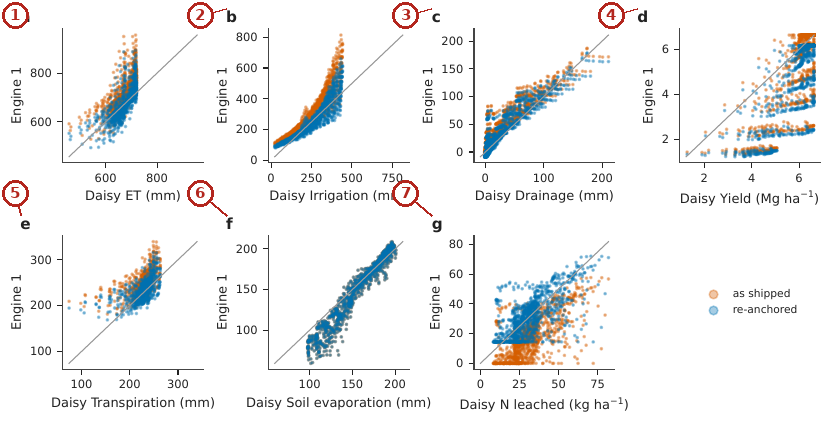
\includegraphics[width=\textwidth,height=0.42\textheight,keepaspectratio]{../figures/annot/p2_fig-e1_0.png}\end{center}

\textbf{What the numbered labels point to.}
\begin{enumerate}[nosep,label=\protect\circled{\arabic*}]
\item Panel (a): ET. \emph{Why:} Points follow the order of Daisy because the meta-model is built from Daisy runs; the offset before re-anchoring comes from anchoring to one reference run.
\item Panel (b): irrigation. \emph{Why:} Points follow the order of Daisy because the meta-model is built from Daisy runs; the offset before re-anchoring comes from anchoring to one reference run.
\item Panel (c): drainage. \emph{Why:} Points follow the order of Daisy because the meta-model is built from Daisy runs; the offset before re-anchoring comes from anchoring to one reference run.
\item Panel (d): yield. \emph{Why:} Points follow the order of Daisy because the meta-model is built from Daisy runs; the offset before re-anchoring comes from anchoring to one reference run.
\item Panel (e): transpiration. \emph{Why:} Points follow the order of Daisy because the meta-model is built from Daisy runs; the offset before re-anchoring comes from anchoring to one reference run.
\item Panel (f): soil evaporation. \emph{Why:} Points follow the order of Daisy because the meta-model is built from Daisy runs; the offset before re-anchoring comes from anchoring to one reference run.
\item Panel (g): nitrogen leached. Grey lines are 1:1. \emph{Why:} Points follow the order of Daisy because the meta-model is built from Daisy runs; the offset before re-anchoring comes from anchoring to one reference run.
\end{enumerate}

\textbf{What it shows.} Engine 1 versus Daisy for the 1\,000 held-out E12 runs. Orange: as shipped; blue: re-anchored. (a) ET, (b) irrigation, (c) drainage, (d) yield, (e) transpiration, (f) soil evaporation, (g) nitrogen leached. Grey lines are 1:1.

\textbf{How to read the labels, symbols and colours.} Engine 1 against Daisy for 1\,000 held-out runs, seven outputs; orange as shipped, blue re-anchored; grey 1:1.

\textbf{What affects it, and why it happens.} Points follow the order of Daisy (good ranking) but are offset as shipped because the meta-model is anchored to one reference run; re-anchoring removes most of the offset.

\textbf{How it is made.} Figure drawn by the script from the input data. Script: \nolinkurl{Manuscripts/reproducibility/analysis/p3_figs.py}. Input: \nolinkurl{Data/daisy_ensemble.csv.gz}.


\subsection{Reading Figure 18 of the article}
\begin{center}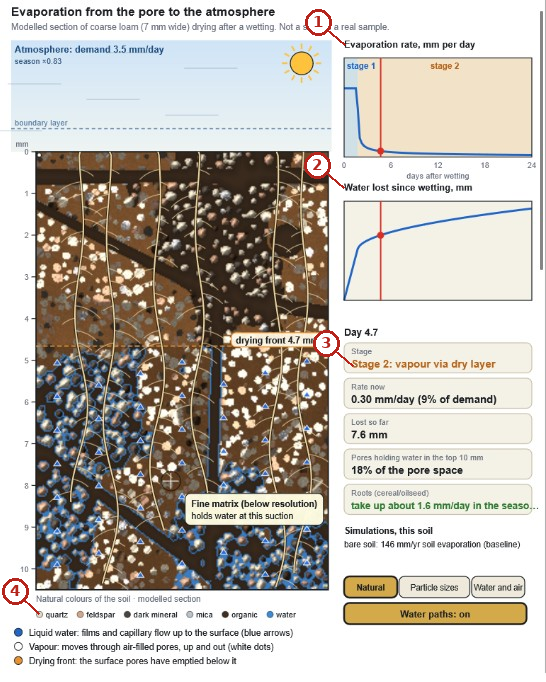
\includegraphics[width=\textwidth,height=0.42\textheight,keepaspectratio]{../figures/annot/p2_fig-shot-layer-e1_0.png}\end{center}

\textbf{What the numbered labels point to (picture 1 of 2: Evaporation from the pore to the atmosphere: a modelled section of coarse loam drying after a wetting, the drying front, stage-1 and stage-2 evaporation and the water lost since wetting (Eq.~(11) and Eq.~(12) of the article)).}
\begin{enumerate}[nosep,label=\protect\circled{\arabic*}]
\item ``Evaporation rate, mm per day'': evaporation from the soil (and, where stated, from mulch or canopy).
\item ``Water lost since wetting'': a heading or control of this screen; the caption above says which layer it belongs to.
\item ``Stage 2: vapour via dry layer'': a heading or control of this screen; the caption above says which layer it belongs to.
\item ``O quartz mineral'': a heading or control of this screen; the caption above says which layer it belongs to.
\end{enumerate}

\begin{center}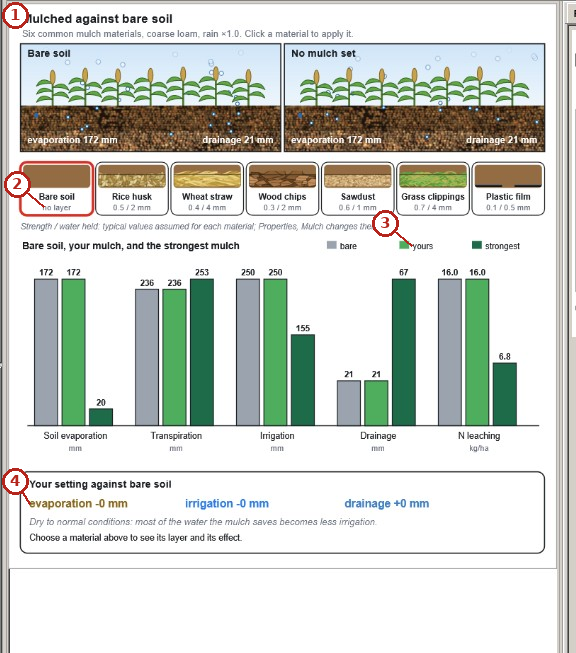
\includegraphics[width=\textwidth,height=0.42\textheight,keepaspectratio]{../figures/annot/p2_fig-shot-layer-e1_1.png}\end{center}

\textbf{What the numbered labels point to (picture 2 of 2: Mulch against bare soil: six mulch materials, and soil evaporation, transpiration, irrigation, drainage and nitrate leaching under bare soil, the chosen mulch and the strongest mulch (Eq.~(13) of the article)).}
\begin{enumerate}[nosep,label=\protect\circled{\arabic*}]
\item ``Mulched against bare soil'': the surface cover and its effect on evaporation.
\item ``no layer'': a heading or control of this screen; the caption above says which layer it belongs to.
\item ``yours'': a heading or control of this screen; the caption above says which layer it belongs to.
\item ``evaporation -0 mm'': evaporation from the soil (and, where stated, from mulch or canopy).
\end{enumerate}

\textbf{What it shows.} SWAFL Desktop: evaporation and mulch. Panels: (a) Evaporation from the pore to the atmosphere: a modelled section of coarse loam drying after a wetting, the drying front, stage-1 and stage-2 evaporation and the water lost since wetting (Eq.~(11) and Eq.~(12) of the article). (b) Mulch against bare soil: six mulch materials, and soil evaporation, transpiration, irrigation, drainage and nitrate leaching under bare soil, the chosen mulch and the strongest mulch (Eq.~(13) of the article).

\textbf{How to read the labels, symbols and colours.} A screen of the software as it appears to the user; the labelled areas are the inputs, the figure and the numbers of the layer named in the caption.

\textbf{What affects it, and why it happens.} Evaporation is fast while the surface is wet (stage 1) and slows when a dry layer forms (stage 2); a mulch reduces the vapour flux through it. 

\textbf{How it is made.} Screen capture of SWAFL Desktop 1.1.0 (not regenerated).


\subsection{Reading Figure 31 of the article}
\begin{center}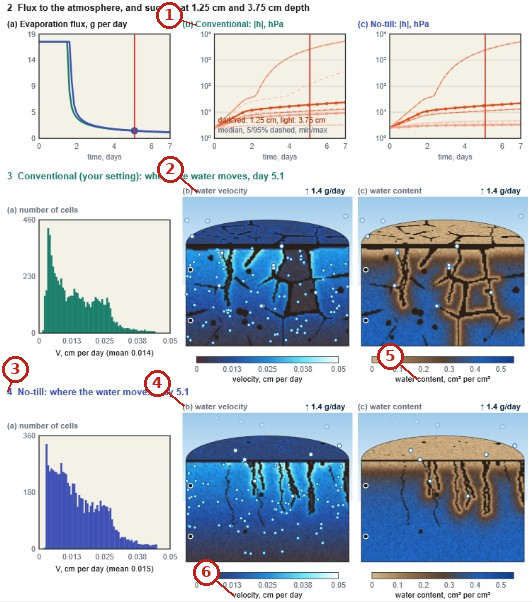
\includegraphics[width=\textwidth,height=0.42\textheight,keepaspectratio]{../figures/annot/p2_fig-shot-real-flux_0.png}\end{center}

\textbf{What the numbered labels point to.}
\begin{enumerate}[nosep,label=\protect\circled{\arabic*}]
\item ``Conventional'': a heading or control of this screen; the caption above says which layer it belongs to.
\item ``water velocity'': a heading or control of this screen; the caption above says which layer it belongs to.
\item ``4 where the water moves'': a heading or control of this screen; the caption above says which layer it belongs to.
\item ``(b) water velocity'': a heading or control of this screen; the caption above says which layer it belongs to.
\item ``content, per cm?'': a heading or control of this screen; the caption above says which layer it belongs to.
\item ``velocity, cm per day'': a rate in millimetres per day.
\end{enumerate}

\textbf{What it shows.} SWAFL Desktop: pore-scale drying of the topsoil under conventional and no tillage: the evaporation flux and the suction at 1.25 and 3.75\,cm, and the distribution, velocity and content of the water on day 5.1 (screen capture of release 1.1.0).

\textbf{How to read the labels, symbols and colours.} A screen of the software as it appears to the user; the labelled areas are the inputs, the figure and the numbers of the layer named in the caption.

\textbf{What affects it, and why it happens.} Under no-till the topsoil keeps more connected pores, so water moves to the surface differently and the suction rises more slowly. 

\textbf{How it is made.} Screen capture of SWAFL Desktop 1.1.0 (not regenerated).

\subsection{Reading Figure 5 of the article}
\begin{center}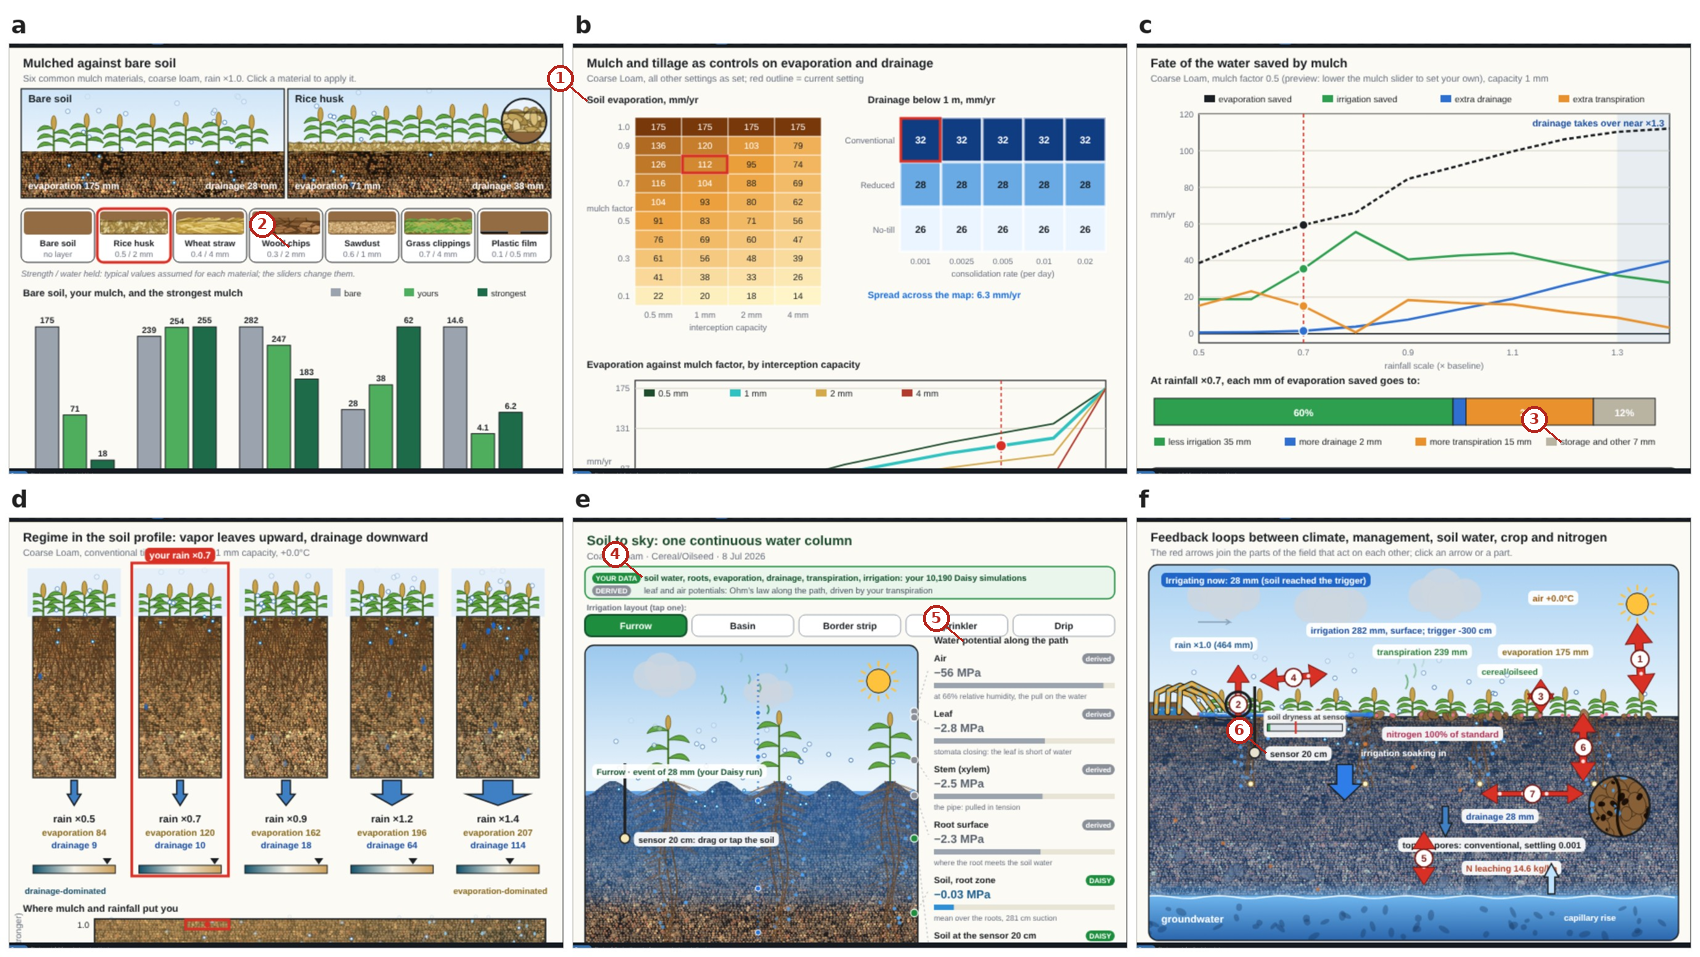
\includegraphics[width=\textwidth,height=0.42\textheight,keepaspectratio]{../figures/annot/p2_fig-viewsC_0.png}\end{center}

\textbf{What the numbered labels point to.}
\begin{enumerate}[nosep,label=\protect\circled{\arabic*}]
\item ``Soil evaporation'': evaporation from the soil (and, where stated, from mulch or canopy).
\item ``chips'': a heading or control of this screen; the caption above says which layer it belongs to.
\item ``storage and other 7 mm'': a heading or control of this screen; the caption above says which layer it belongs to.
\item ``soil water, roots, evaporation'': evaporation from the soil (and, where stated, from mulch or canopy).
\item ``potential along the path'': a heading or control of this screen; the caption above says which layer it belongs to.
\item ``sensor'': the soil-water sensor: its depth and reading.
\end{enumerate}

\textbf{What it shows.} Result views for mulch and the whole system. (a) Mulch against bare soil; (b) mulch strength; (c) fate of the saved water; (d) regime map of where mulch pays; (e) soil to sky; (f) how the effects connect.

\textbf{How to read the labels, symbols and colours.} Views for mulch and the whole system.

\textbf{What affects it, and why it happens.} A mulch lowers evaporation and catches rain; where the saving goes depends on how fast the soil drains. A mulch reduces evaporation, intercepts rain and warms the soil; where the saving goes depends on the soil's drainage.

\textbf{How it is made.} Screen capture of SWAFL Desktop 1.1.0 (not regenerated).


\subsection{Reading Figure 19 of the article}
\begin{center}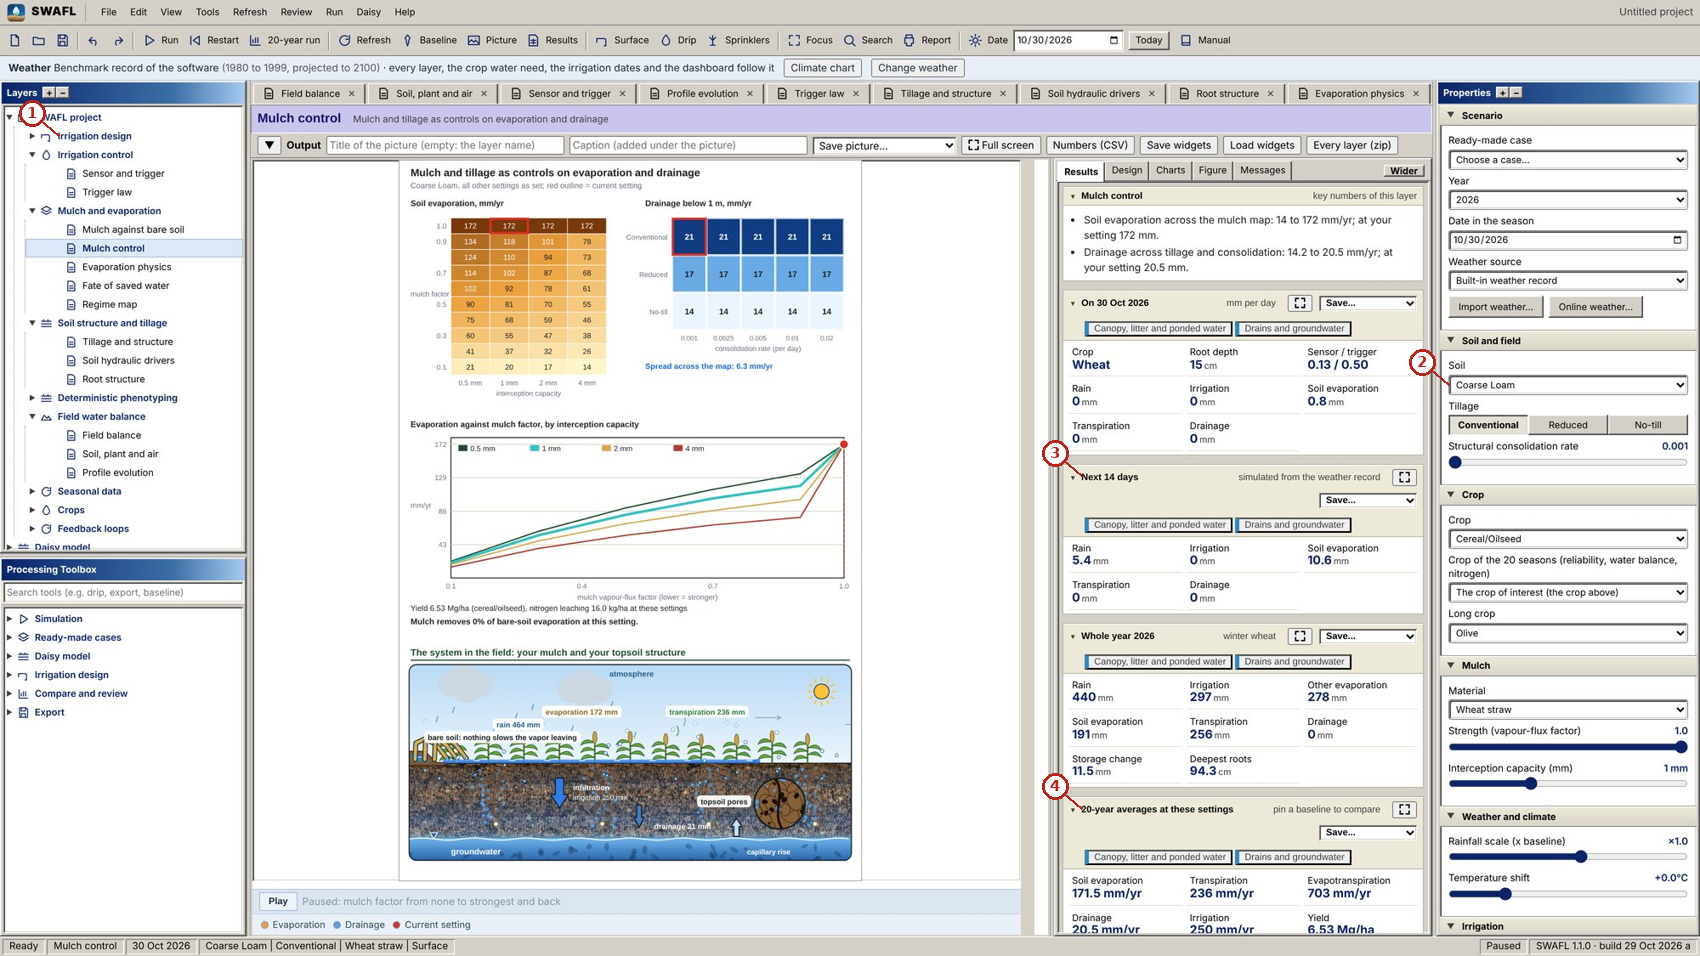
\includegraphics[width=\textwidth,height=0.42\textheight,keepaspectratio]{../figures/annot/p2_fig-shot-layer-v6_0.png}\end{center}

\textbf{What the numbered labels point to (picture 1 of 2: Mulch control: soil evaporation by mulch factor and interception capacity, and drainage by tillage and consolidation rate.).}
\begin{enumerate}[nosep,label=\protect\circled{\arabic*}]
\item ``Irrigation design'': the irrigation-design group of the Layers tree and its layers.
\item ``coarse Loam'': the soil of the project, which every layer uses.
\item ``Next 14 days'': the decision for the next 14 days, from the soil water of the day.
\item ``20-year averages at these settings'': a heading or control of this screen; the caption above says which layer it belongs to.
\end{enumerate}

\begin{center}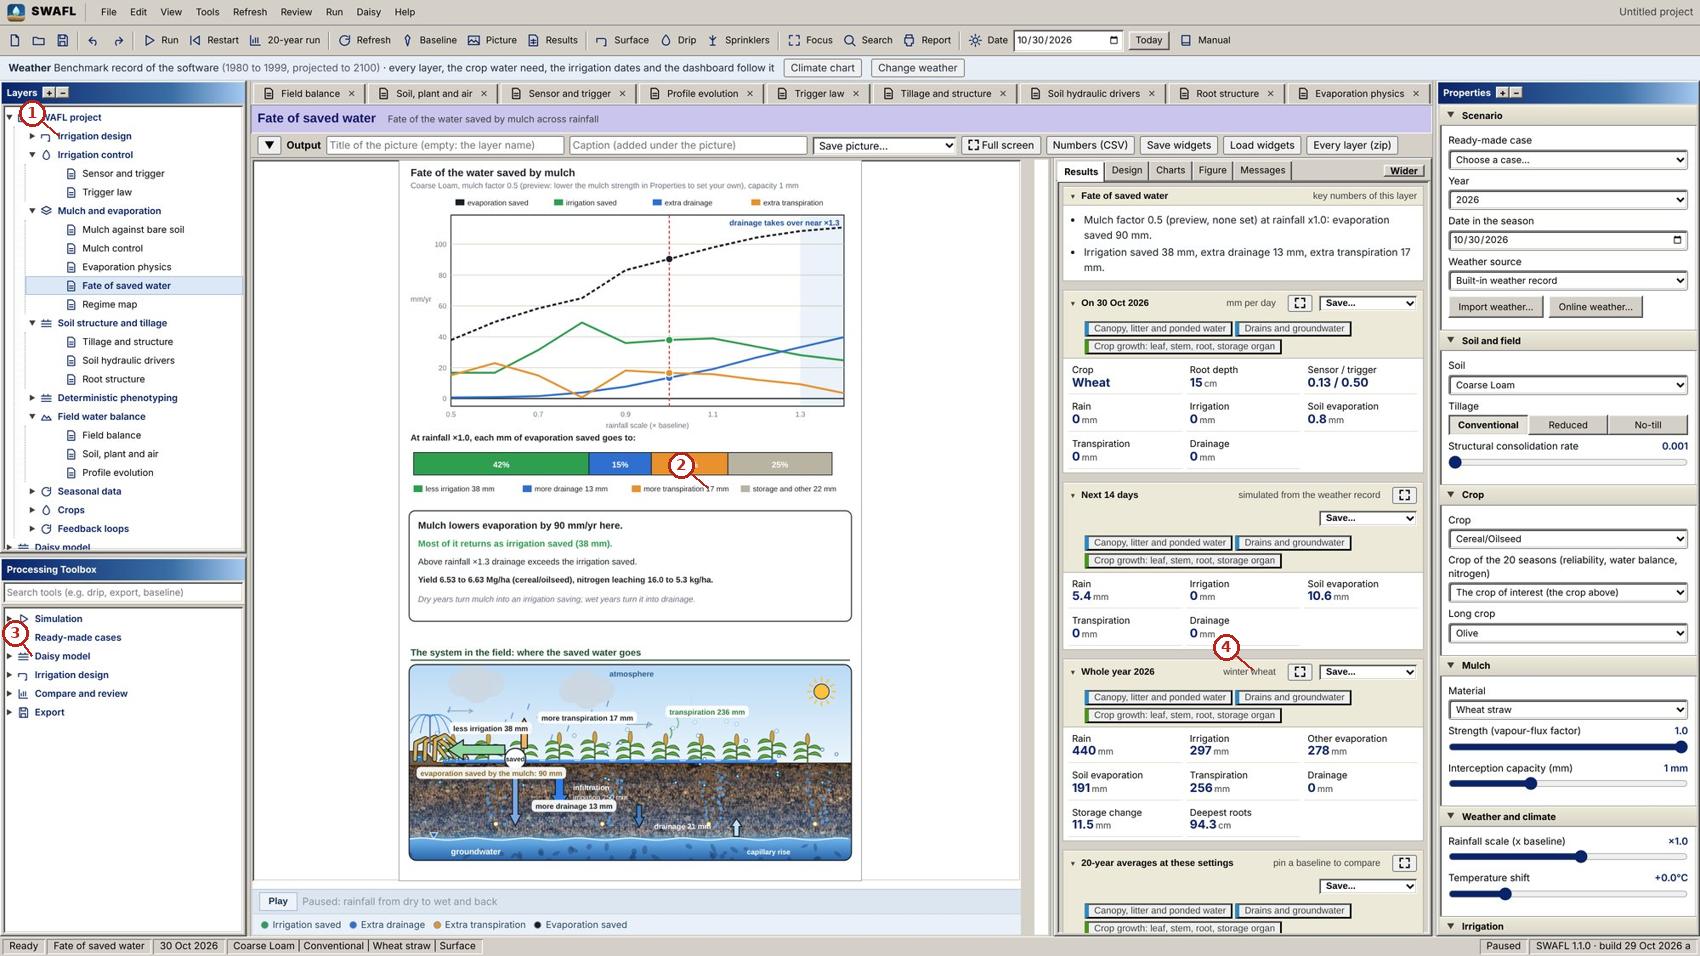
\includegraphics[width=\textwidth,height=0.42\textheight,keepaspectratio]{../figures/annot/p2_fig-shot-layer-v6_1.png}\end{center}

\textbf{What the numbered labels point to (picture 2 of 2: Fate of saved water: evaporation saved, irrigation saved, extra drainage and extra transpiration against the rainfall scale (Eq.~(23) of the article).).}
\begin{enumerate}[nosep,label=\protect\circled{\arabic*}]
\item ``Irrigation design'': the irrigation-design group of the Layers tree and its layers.
\item ``17 mm storage and other 22'': a heading or control of this screen; the caption above says which layer it belongs to.
\item ``Daisy'': the Daisy model and its workbench.
\item ``wheat'': the crop of the project and its stage.
\end{enumerate}

\textbf{What it shows.} SWAFL Desktop: mulch control and the fate of saved water. Panels: (a) Mulch control: soil evaporation by mulch factor and interception capacity, and drainage by tillage and consolidation rate. (b) Fate of saved water: evaporation saved, irrigation saved, extra drainage and extra transpiration against the rainfall scale (Eq.~(23) of the article).

\textbf{How to read the labels, symbols and colours.} A screen of the software as it appears to the user; the labelled areas are the inputs, the figure and the numbers of the layer named in the caption.

\textbf{What affects it, and why it happens.} The water a mulch saves goes to transpiration, less irrigation or drainage, in shares set by the soil. 

\textbf{How it is made.} Screen capture of SWAFL Desktop 1.1.0 (not regenerated).


\subsection{Reading Figure 20 of the article}
\begin{center}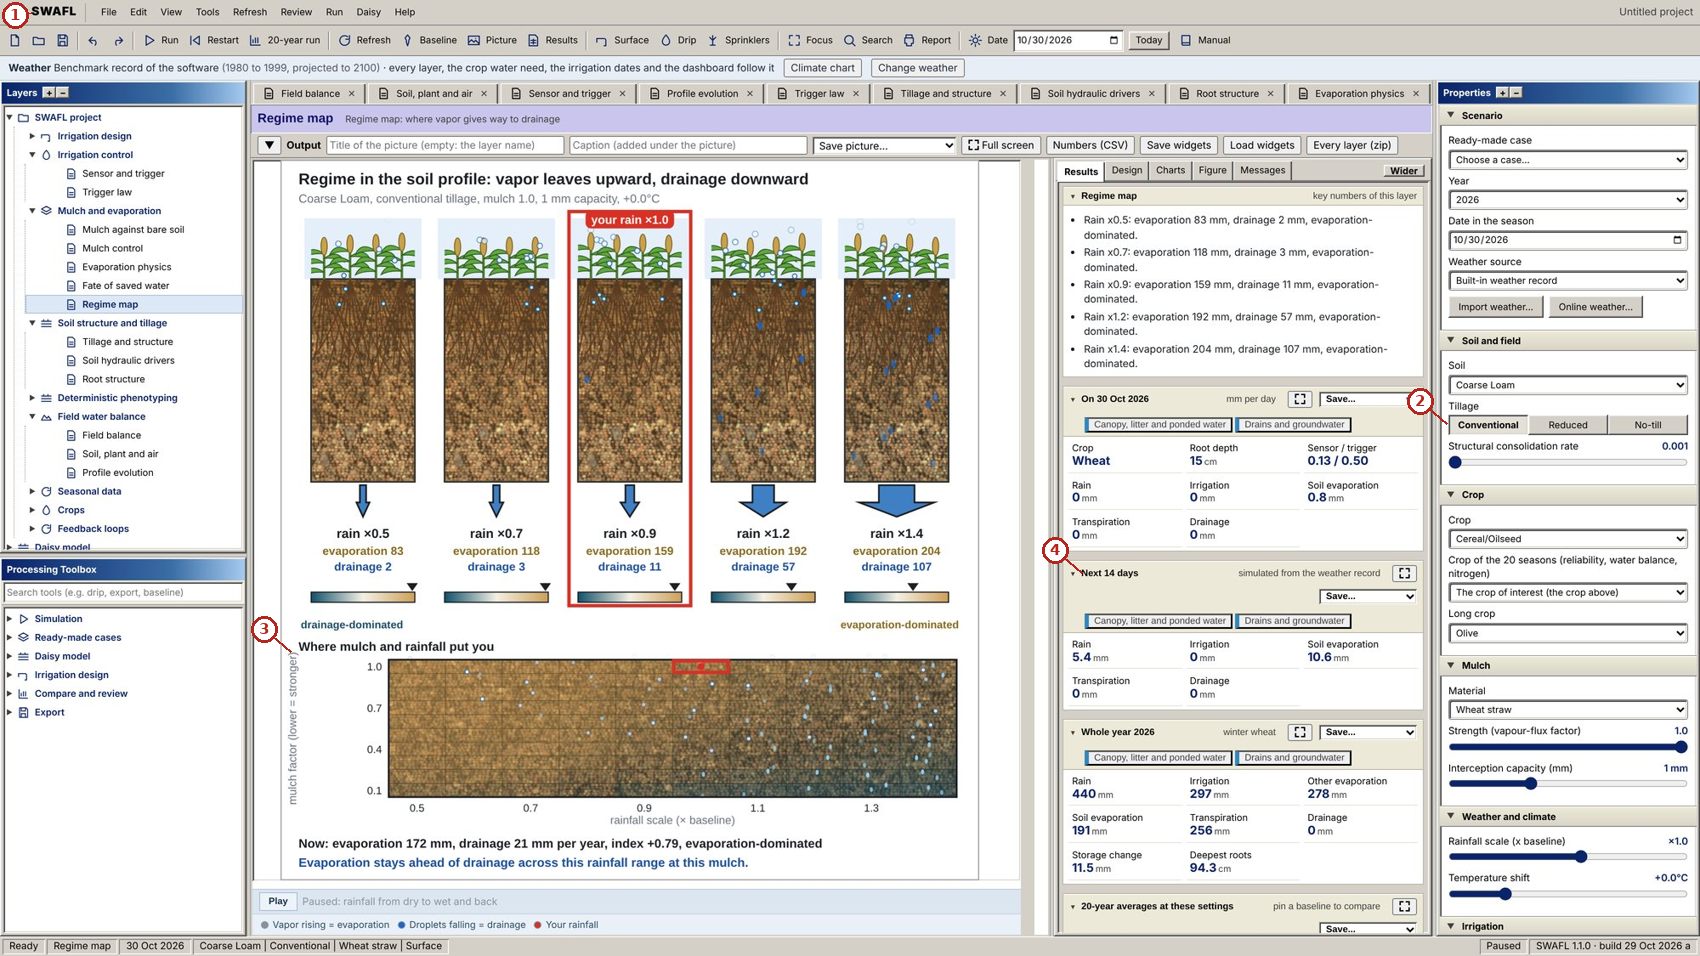
\includegraphics[width=\textwidth,height=0.42\textheight,keepaspectratio]{../figures/annot/p2_fig-shot-layer-n3_0.png}\end{center}

\textbf{What the numbered labels point to (picture 1 of 2: Regime map: mulch factor against rainfall scale coloured by the dominant loss (Eq.~(14) of the article).).}
\begin{enumerate}[nosep,label=\protect\circled{\arabic*}]
\item ``SWAFL View Run Daisy Help'': the menu bar of the program (file, view, run, Daisy, help).
\item ``No-till'': a heading or control of this screen; the caption above says which layer it belongs to.
\item ``Where mulch and rainfall pat you'': rain, from the weather of the project.
\item ``Next 14 days'': the decision for the next 14 days, from the soil water of the day.
\end{enumerate}

\begin{center}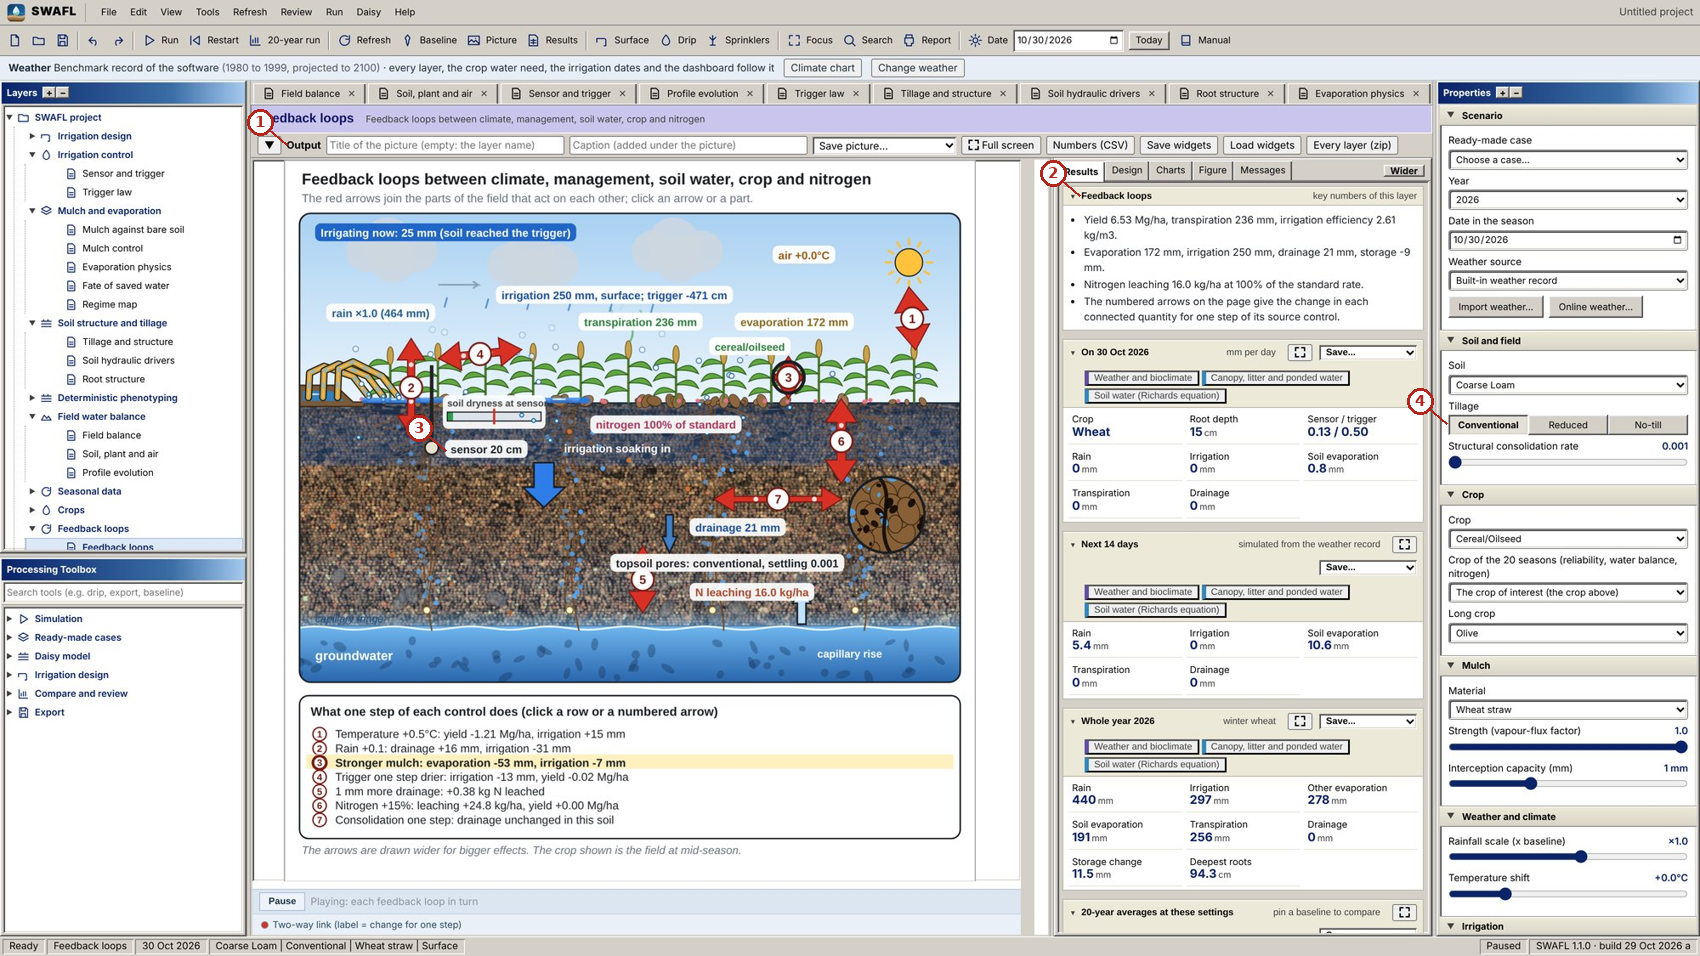
\includegraphics[width=\textwidth,height=0.42\textheight,keepaspectratio]{../figures/annot/p2_fig-shot-layer-n3_1.png}\end{center}

\textbf{What the numbered labels point to (picture 2 of 2: Feedback loops: the seven loops with arrow widths scaled by the effect of one control step (Table~4 of the article).).}
\begin{enumerate}[nosep,label=\protect\circled{\arabic*}]
\item ``Output'': the output bar of the layer: title and caption of the picture, save the picture, full screen, numbers as CSV.
\item ``Feedback loops'': the feedback loops between climate, management, soil water, crop and nitrogen.
\item ``sensor 20 cm'': the soil-water sensor: its depth and reading.
\item ``No-till'': a heading or control of this screen; the caption above says which layer it belongs to.
\end{enumerate}

\textbf{What it shows.} SWAFL Desktop: regime map and feedback loops. Panels: (a) Regime map: mulch factor against rainfall scale coloured by the dominant loss (Eq.~(14) of the article). (b) Feedback loops: the seven loops with arrow widths scaled by the effect of one control step (Table~4 of the article).

\textbf{How to read the labels, symbols and colours.} A screen of the software as it appears to the user; the labelled areas are the inputs, the figure and the numbers of the layer named in the caption.

\textbf{What affects it, and why it happens.} The regime map shows where the saved water drains (coarse soils, wet climate) and where it is used. 

\textbf{How it is made.} Screen capture of SWAFL Desktop 1.1.0 (not regenerated).


\subsection{Derivation: Consolidation of the tilled layer}\label{der:s2:4}
If the excess pore space decays at a rate proportional to itself, $\dd p/\dd t=-\tau_c(p-p_c)$, then $p(t)=p_c+(p_0-p_c)e^{-\tau_ct}$, with $p_0$ set by the tillage and $p_c$ the consolidated state.


\subsection{Derivation: Two-stage evaporation}\label{der:s2:5}
In stage 1 the surface is wet and evaporation runs at the demand $e_0$, so $Q=q_0+e_0t$ until the cumulative stage-1 limit $Q_1$ is reached at $t_1=(Q_1-q_0)/e_0$. In stage 2 evaporation is limited by diffusion through the dry layer; for a desorptivity-controlled flux $e=S/(2\sqrt{t})$ the cumulative loss grows as $\sqrt t$. The form of the paper, $Q=Q_1+2e_0\tau_E(\sqrt{1+(t-t_1)/\tau_E}-1)$, starts stage 2 at the stage-1 rate (its derivative at $t=t_1$ is $e_0$) and tends to the $\sqrt t$ law for $t-t_1\gg\tau_E$, which joins the two stages smoothly \citep{Ritchie1972,Philip1957}.


\subsection{Derivation: Water potential of the air}\label{der:s2:6}
For water vapour in equilibrium with liquid water, the chemical potential difference per unit volume is $\psi=(\mathcal R T_K/V_w)\ln\mathrm{RH}$ (Kelvin). At 20\,$^\circ$C, $\mathcal RT_K/V_w=8.314\times293.15/1.8\times10^{-5}=1.353\times10^{8}$\,Pa, that is $135.3$\,MPa, so $\psi_{\mathrm{air}}\simeq135.3\ln\mathrm{RH}$\,MPa.


\subsection{Derivation: The soil--plant--atmosphere path}\label{der:s2:7}
With steady flow $q$ through soil, root, xylem and leaf in series, each segment drops the potential by $qR_j$ (the van den Honert analogue of Ohm's law), so $\psi_{\mathrm{leaf}}=\psi_{\mathrm{RZ}}-q(R_{\mathrm{soil}}+R_{\mathrm{root}}+R_{\mathrm{xyl}}+R_{\mathrm{leaf}})$. The soil resistance grows as the conductivity falls; bounding $K_r$ from below (the floor of the paper) bounds $R_{\mathrm{soil}}$ and therefore the leaf potential, which is why that potential is set by the floor rather than by the soil when the soil is dry.


\subsection{Why it happens}
\paragraph{Why stage-1 evaporation lasts longer in fine soils.} Fine soils hold more water near the surface and conduct it upward over longer distances, so the surface stays wet longer.

\paragraph{Why the leaf water potential is set by a conductivity floor.} The series resistance of the soil grows without bound as the soil dries; the software bounds the relative conductivity from below to keep the calculation finite, and in dry soil that bound, not the soil, then decides the leaf potential.

\paragraph{Why the drainage share of a mulch saving is understated in coarse soils.} The engines split the saving with ratios that do not contain the soil's drainage competition; in coarse soils, where most saved water drains, that split gives too little to drainage.

\section{The model, its equations and its views}
The architecture, the ledger of equations and the result views.

\subsection{Contribution 4: a ledger of every equation}\label{con:s2:4}
\begin{keyresult}
\centering\small
\begin{tabular}{lrl}
\toprule
Origin & Equations & Meaning\\\midrule
\circled{1}\ Literature & 38 & taken from a cited source\\
\circled{2}\ Fitted to data & 18 & coefficients fitted to the ensemble\\
\circled{3}\ Engineered & 78 & form chosen for the software\\\bottomrule
\end{tabular}
\end{keyresult}
\begin{pins}
\pin{1}{These carry the authority of their source and need only to be implemented correctly.}
\pin{2}{These hold only within the data they were fitted to; their range is stated.}
\pin{3}{These are the largest class and the ones that most need testing; labelling them tells the reader where the evidence is weakest.}
\end{pins}


\subsection{Reading Figure 1 of the article}
\begin{center}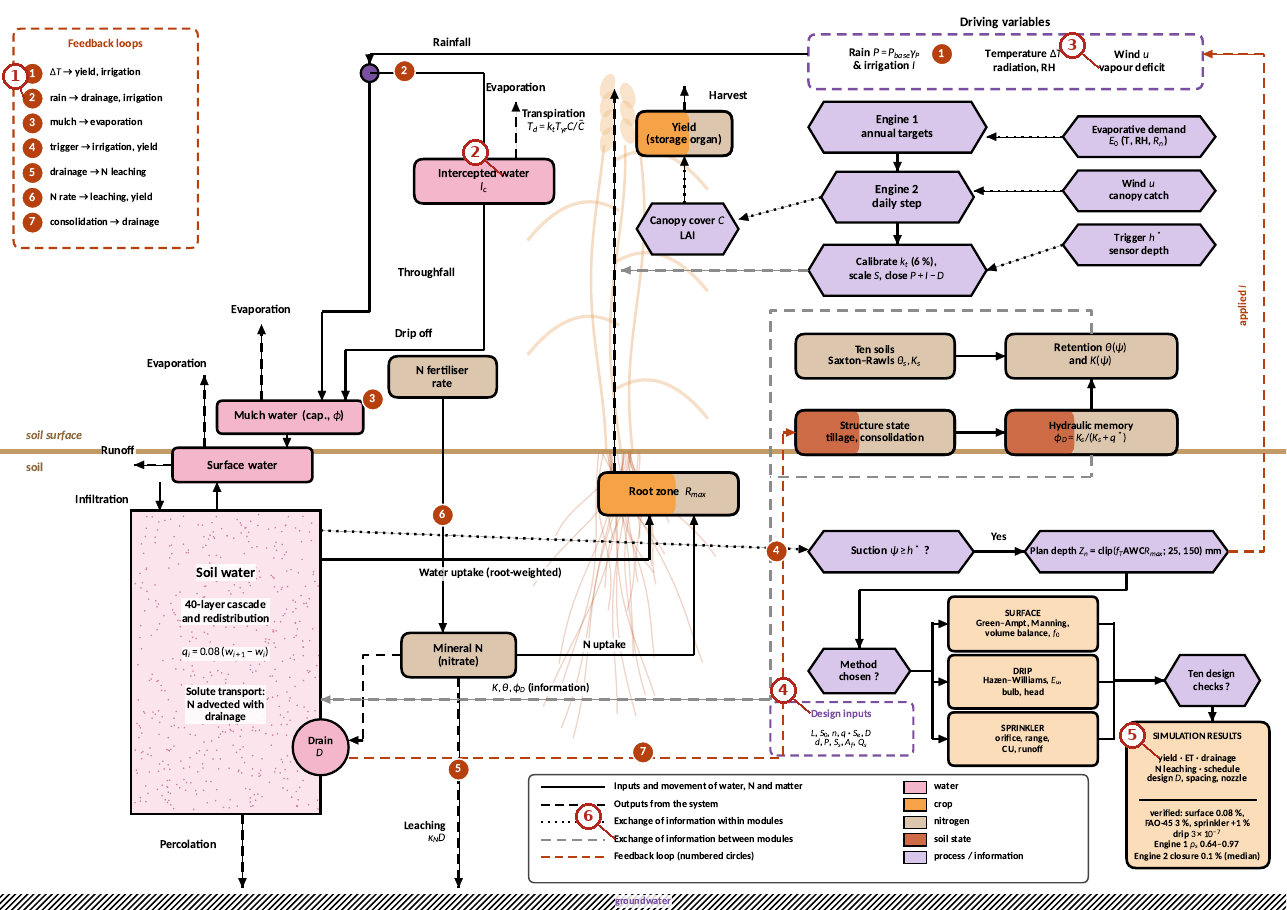
\includegraphics[width=\textwidth,height=0.42\textheight,keepaspectratio]{../figures/annot/p2_fig-arch_0.png}\end{center}

\textbf{What the numbered labels point to.}
\begin{enumerate}[nosep,label=\protect\circled{\arabic*}]
\item ``drainage'': rain, from the weather of the project.
\item ``water'': a heading or control of this screen; the caption above says which layer it belongs to.
\item ``vapour deficit'': a heading or control of this screen; the caption above says which layer it belongs to.
\item ``Design inputs'': a heading or control of this screen; the caption above says which layer it belongs to.
\item ``yield ET - drainage'': rain, from the weather of the project.
\item ``Exchange of information between modules'': a heading or control of this screen; the caption above says which layer it belongs to.
\end{enumerate}

\textbf{What it shows.} Schematic overview of the main processes in SWAFL Desktop. Boxes indicate storages and solid lines flows; dashed black lines are flows out of the system, dotted lines are flows of information and dashed grey lines exchange of information between modules. Dashed purple boxes with a triangle are the drop-down controls and driving variables of the Properties panel, and the drivers of soil hydraulic properties (SHP). Dashed red lines and numbered circles mark the seven feedback loops. Pink indicates water, orange the crop, light brown nitrogen and rust soil structure and hydraulic state; purple hexagons are processes and information (Engines~1 and 2, trigger, design layers) and peach boxes are design layers and results. The brown line is the soil surface, with groundwater hatched at the base.

\textbf{How to read the labels, symbols and colours.} Boxes are storages, solid lines flows, dotted lines information; dashed purple boxes the controls; red dashed lines with numbers the seven feedback loops; pink water, orange crop, brown nitrogen, rust structure.

\textbf{What affects it, and why it happens.} The diagram shows how one control (for example the trigger) reaches every output through the coupled flows and feedbacks.

\textbf{How it is made.} Figure drawn by the script from the input data. Script: \nolinkurl{Manuscripts/reproducibility/make_a4.py}. Input: \nolinkurl{Data/daisy_ensemble.csv.gz}.


\subsection{Reading Figure 3 of the article}
\begin{center}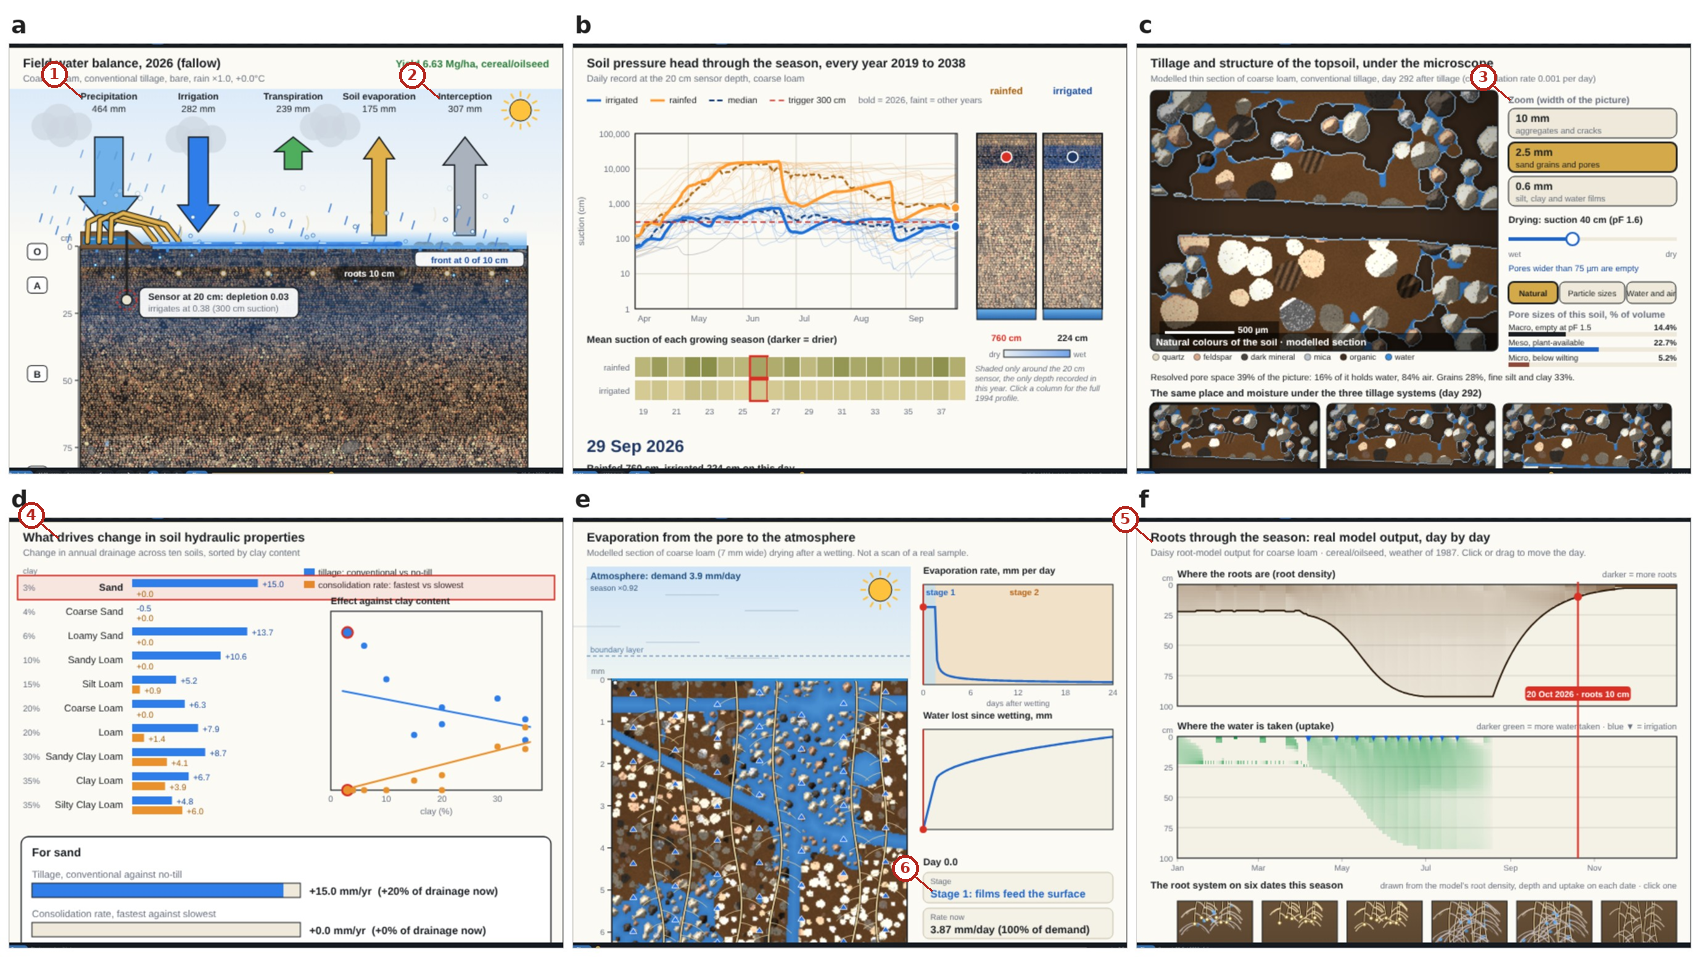
\includegraphics[width=\textwidth,height=0.42\textheight,keepaspectratio]{../figures/annot/p2_fig-viewsA_0.png}\end{center}

\textbf{What the numbered labels point to.}
\begin{enumerate}[nosep,label=\protect\circled{\arabic*}]
\item ``Precipitation'': rain, from the weather of the project.
\item ``Interception'': a heading or control of this screen; the caption above says which layer it belongs to.
\item ``Zoom (width of the picture)'': a heading or control of this screen; the caption above says which layer it belongs to.
\item ``drives change in soil properties'': the soil of the project, which every layer uses.
\item ``Roots through the season: real model'': the roots: depth, density and uptake.
\item ``stage 1: films feed the surface'': a heading or control of this screen; the caption above says which layer it belongs to.
\end{enumerate}

\textbf{What it shows.} Result views of the explorer for the soil and the field (coarse loam, conventional tillage, cereal rotation). (a) Field water balance of the root zone; (b) soil-water pressure-head profile; (c) pores and tillage; (d) soil hydraulic drivers by texture; (e) evaporation from the pore to the atmosphere; (f) root density and uptake. Governing relations are listed in Table~11 of the article.

\textbf{How to read the labels, symbols and colours.} Six result views of the program (field balance, pressure-head profile, pores and tillage, hydraulic drivers, evaporation, roots).

\textbf{What affects it, and why it happens.} Each view draws one relation of the engines for the soil chosen; a different soil changes every view at once. Each view draws one relation of the engines for the chosen soil; changing the soil or a control moves all of them together.

\textbf{How it is made.} Screen capture of SWAFL Desktop 1.1.0 (not regenerated).


\subsection{Reading Figure 12 of the article}
\begin{center}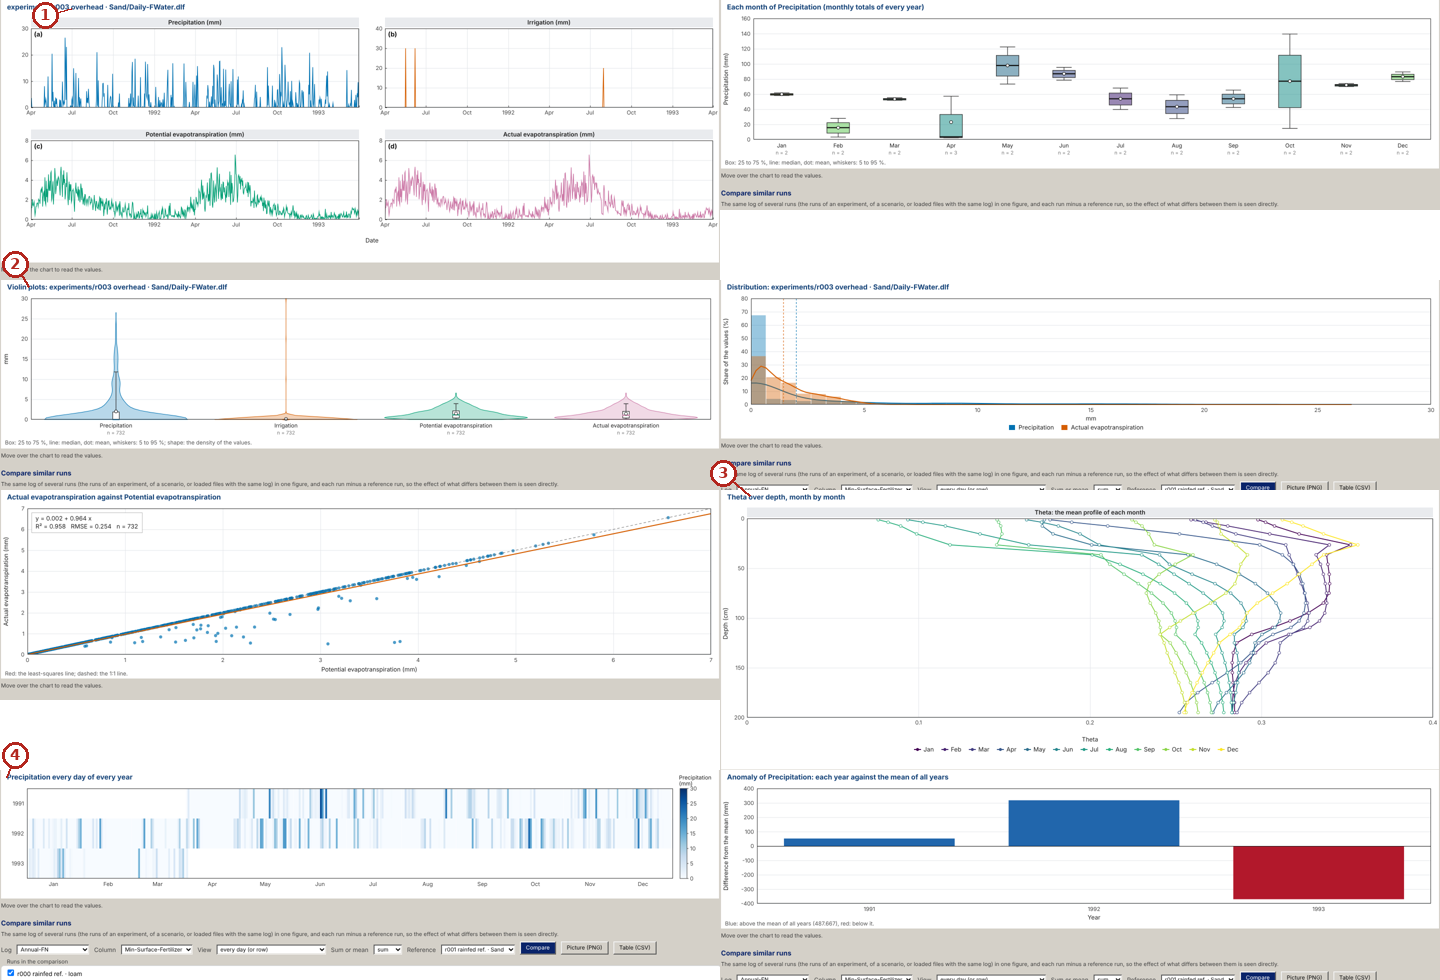
\includegraphics[width=\textwidth,height=0.42\textheight,keepaspectratio]{../figures/annot/p2_fig-plotviews_0.png}\end{center}

\textbf{What the numbered labels point to.}
\begin{enumerate}[nosep,label=\protect\circled{\arabic*}]
\item ``overhead'': a heading or control of this screen; the caption above says which layer it belongs to.
\item ``plots: experiments/r003 overhead'': a heading or control of this screen; the caption above says which layer it belongs to.
\item ``over depth, month by month'': a heading or control of this screen; the caption above says which layer it belongs to.
\item ``Precipitation every day of every year'': rain, from the weather of the project.
\end{enumerate}

\textbf{What it shows.} Eight of the twenty kinds of figure of the Log plots of release 1.1.0, drawn from the daily logs of one Daisy run: small multiples, monthly box plots, violin plots, histogram with density, scatter with the least-squares line, R$^2$ and RMSE, the mean profile of each month, a calendar heat map and the anomaly of each year (screen captures).

\textbf{How to read the labels, symbols and colours.} Eight kinds of figure drawn from the daily logs of one run (small multiples, monthly boxes, violins, histogram, scatter with fit, monthly profile, calendar map, yearly anomaly).

\textbf{What affects it, and why it happens.} Each kind of plot shows the same daily log differently: through time, spread within months, distribution, relation to another quantity, departure of each year. Each shows the same log in a different way: course in time, spread within months, distribution, relation to another quantity and departure of each year from the mean.

\textbf{How it is made.} Screen capture of SWAFL Desktop 1.1.0 (not regenerated).


\subsection{Reading Figure 13 of the article}
\begin{center}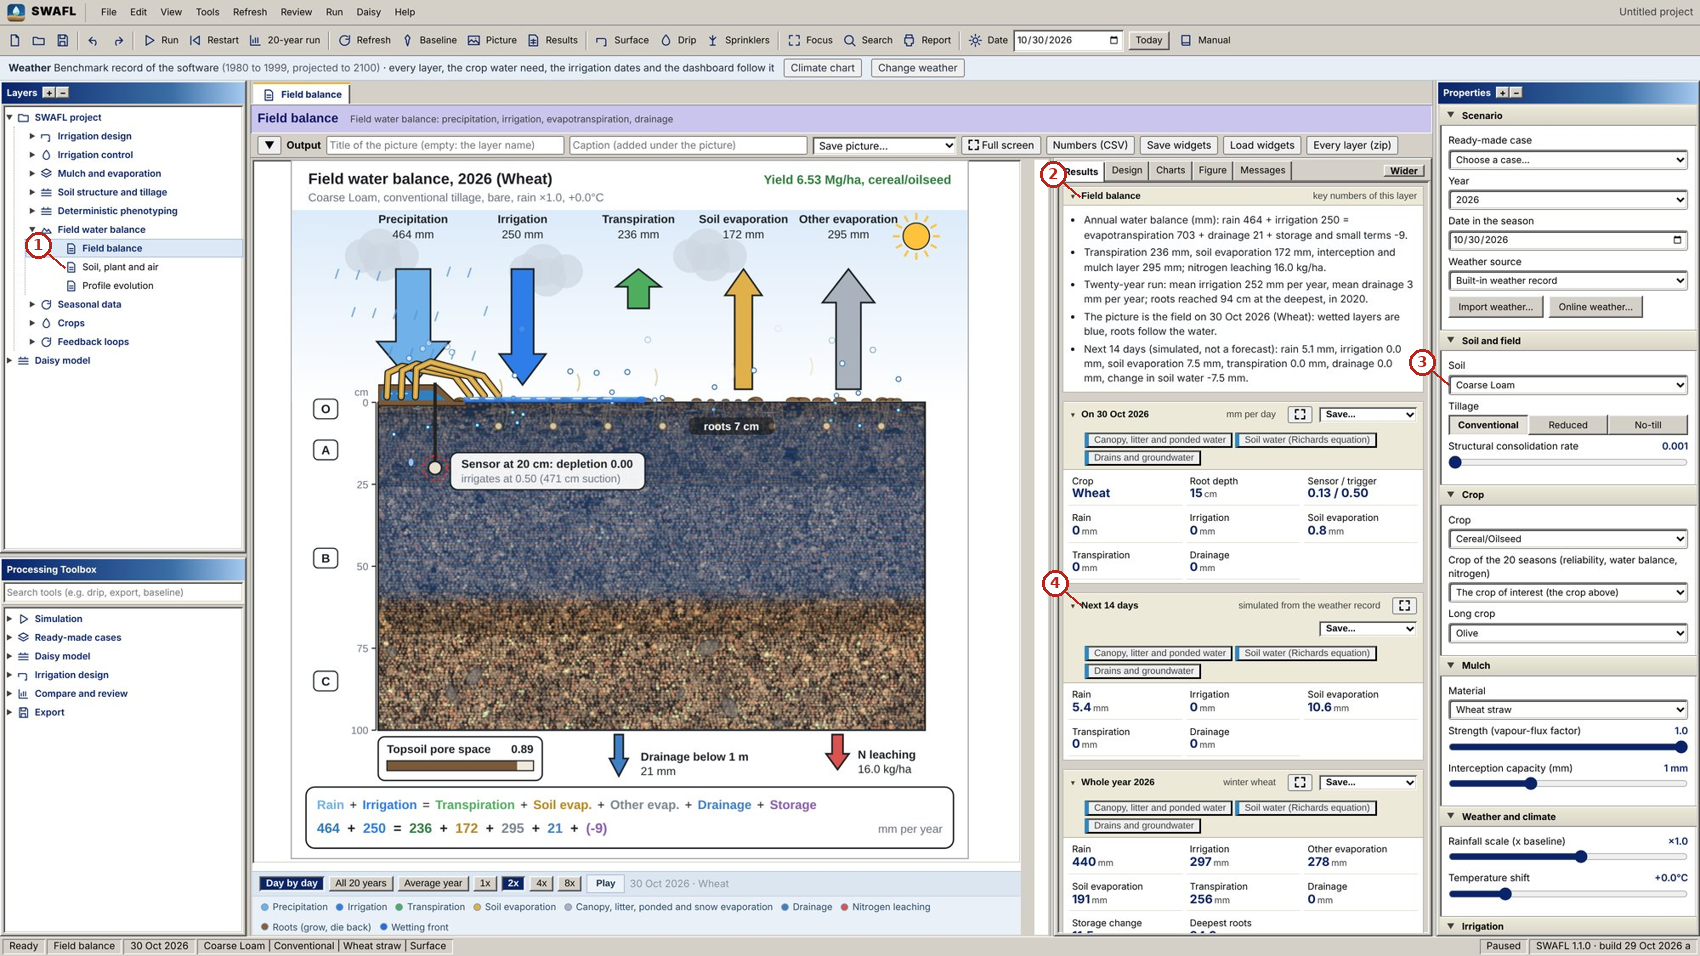
\includegraphics[width=\textwidth,height=0.42\textheight,keepaspectratio]{../figures/annot/p2_fig-shot-layer-field_0.png}\end{center}

\textbf{What the numbered labels point to (picture 1 of 2: Field balance, the home view: daily fluxes on the field clock, the soil profile with sensor, roots and wetting front, and the closed budget (Eq.~(1) of the article).).}
\begin{enumerate}[nosep,label=\protect\circled{\arabic*}]
\item ``Soil, and air'': the soil of the project, which every layer uses.
\item ``Field balance'': the field water balance: inputs, outputs and storage of the root zone.
\item ``Coarse Loam v'': the soil of the project, which every layer uses.
\item ``Next 14 days'': the decision for the next 14 days, from the soil water of the day.
\end{enumerate}

\begin{center}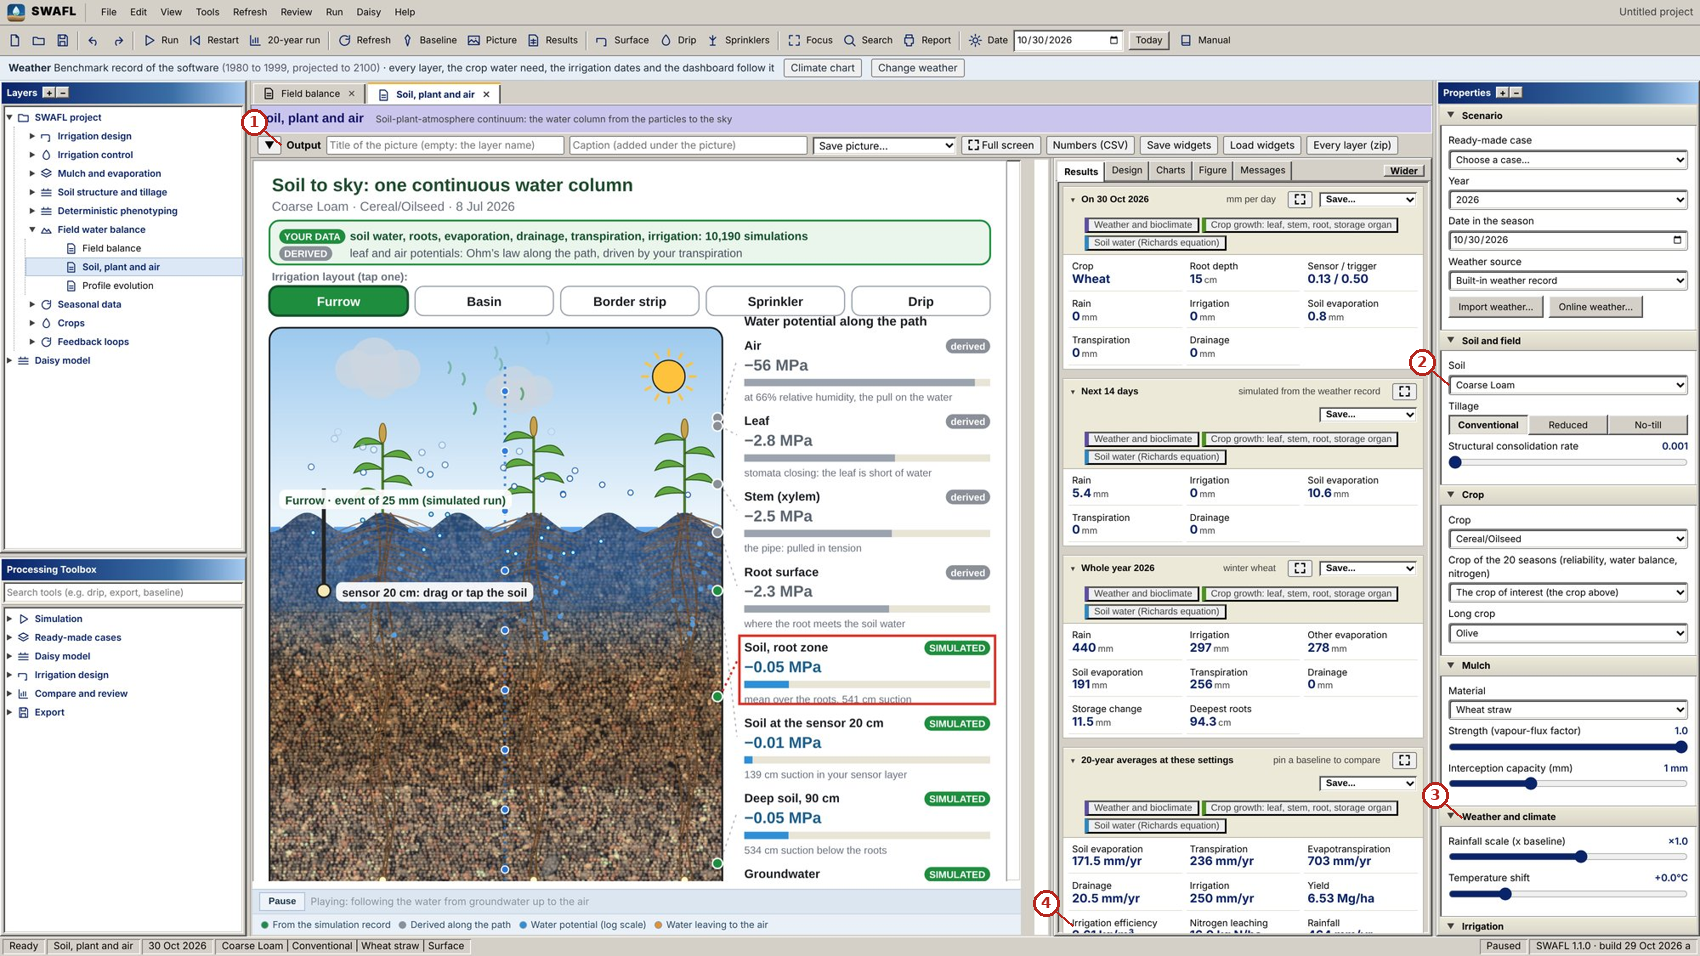
\includegraphics[width=\textwidth,height=0.42\textheight,keepaspectratio]{../figures/annot/p2_fig-shot-layer-field_1.png}\end{center}

\textbf{What the numbered labels point to (picture 2 of 2: Soil, plant and air: layouts of the five irrigation methods and the water potential along the path from the deep soil to the air (Eq.~(21) and Eq.~(22) and Eq.~(15) of the article).).}
\begin{enumerate}[nosep,label=\protect\circled{\arabic*}]
\item ``Output'': the output bar of the layer: title and caption of the picture, save the picture, full screen, numbers as CSV.
\item ``Coarse Loam v'': the soil of the project, which every layer uses.
\item ``Weather and climate'': the weather of the project: built-in record, a file of the user or online weather of any place.
\item ``Irrigation efficiency'': a heading or control of this screen; the caption above says which layer it belongs to.
\end{enumerate}

\textbf{What it shows.} SWAFL Desktop: field and the soil--plant--air path. Panels: (a) Field balance, the home view: daily fluxes on the field clock, the soil profile with sensor, roots and wetting front, and the closed budget (Eq.~(1) of the article). (b) Soil, plant and air: layouts of the five irrigation methods and the water potential along the path from the deep soil to the air (Eq.~(21) and Eq.~(22) and Eq.~(15) of the article).

\textbf{How to read the labels, symbols and colours.} A screen of the software as it appears to the user; the labelled areas are the inputs, the figure and the numbers of the layer named in the caption.

\textbf{What affects it, and why it happens.} The field balance adds the day's rain and irrigation and subtracts evaporation, transpiration and drainage; the path from soil to air shows the potential falling through each resistance, which is why the leaf is much drier than the soil. 

\textbf{How it is made.} Screen capture of SWAFL Desktop 1.1.0 (not regenerated).


\subsection{Reading Figure 28 of the article}
\begin{center}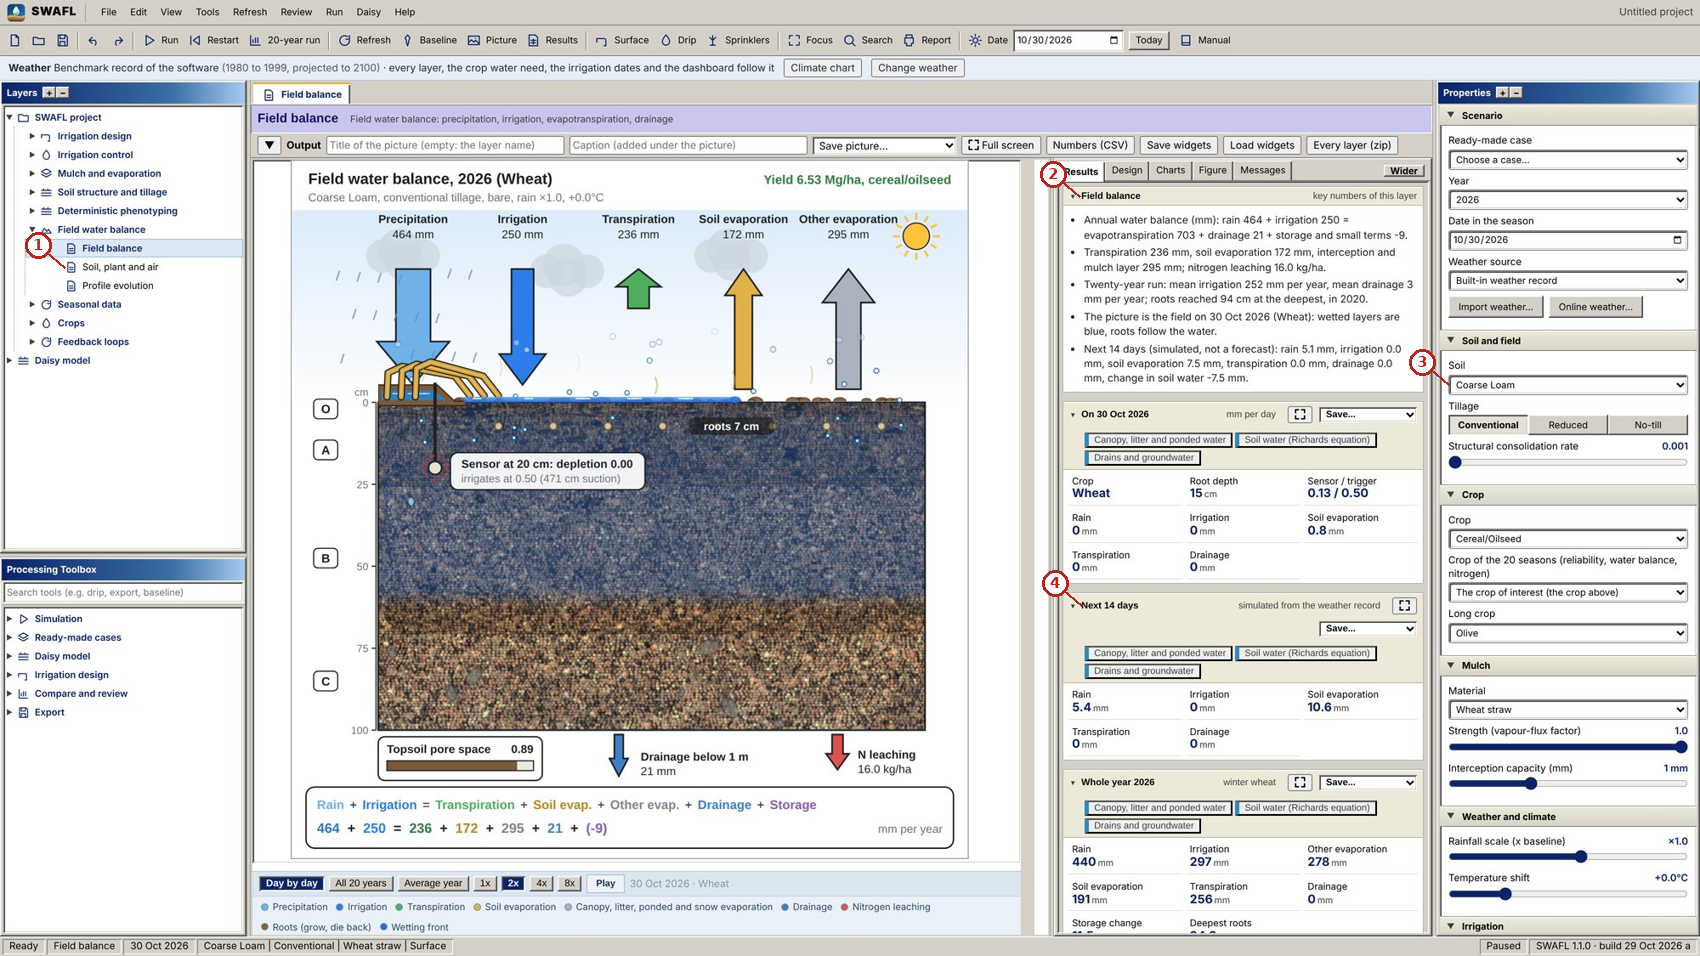
\includegraphics[width=\textwidth,height=0.42\textheight,keepaspectratio]{../figures/annot/p2_fig-shot-dash-results_0.png}\end{center}

\textbf{What the numbered labels point to (picture 1 of 2: Dashboard, results tab: annual and daily flux tiles of the field water balance.).}
\begin{enumerate}[nosep,label=\protect\circled{\arabic*}]
\item ``Soil, and air'': the soil of the project, which every layer uses.
\item ``Field balance'': the field water balance: inputs, outputs and storage of the root zone.
\item ``Coarse Loam v'': the soil of the project, which every layer uses.
\item ``Next 14 days'': the decision for the next 14 days, from the soil water of the day.
\end{enumerate}

\begin{center}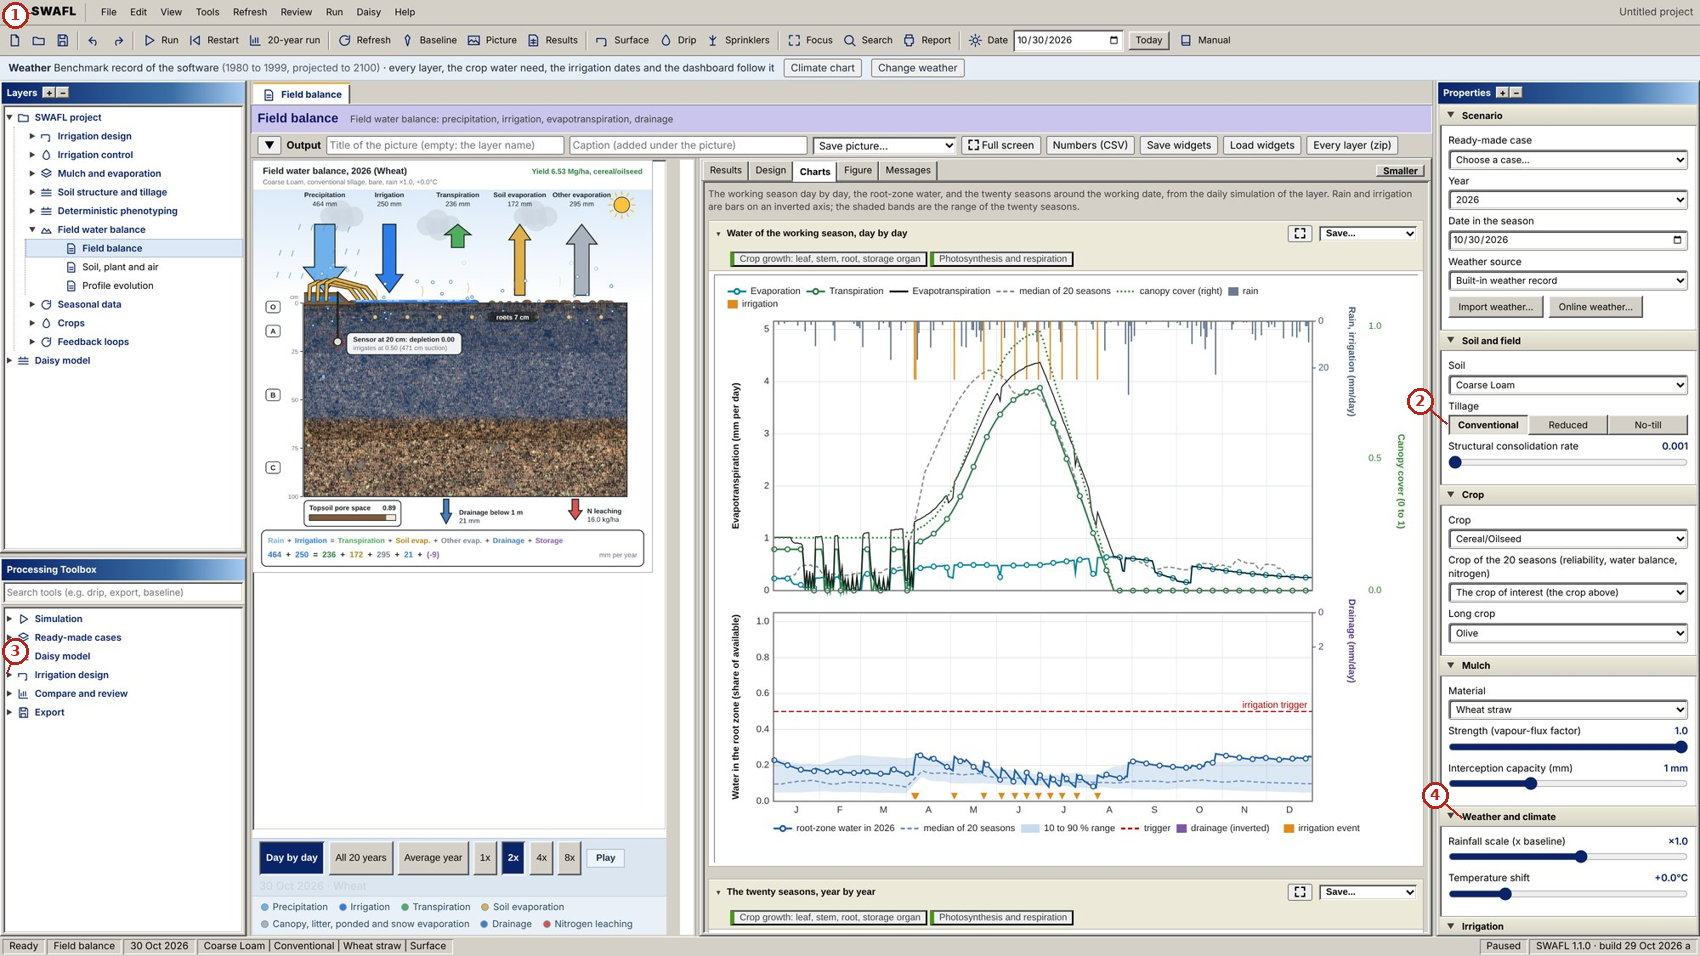
\includegraphics[width=\textwidth,height=0.42\textheight,keepaspectratio]{../figures/annot/p2_fig-shot-dash-results_1.png}\end{center}

\textbf{What the numbered labels point to (picture 2 of 2: Dashboard, charts tab: seasonal rainfall, irrigation, drainage, evaporation and transpiration.).}
\begin{enumerate}[nosep,label=\protect\circled{\arabic*}]
\item ``SWAFL View Run Daisy Help'': the menu bar of the program (file, view, run, Daisy, help).
\item ``No-till'': a heading or control of this screen; the caption above says which layer it belongs to.
\item ``Irrigation design'': the irrigation-design group of the Layers tree and its layers.
\item ``Weather and climate'': the weather of the project: built-in record, a file of the user or online weather of any place.
\end{enumerate}

\textbf{What it shows.} SWAFL Desktop: dashboard. Panels: (a) Dashboard, results tab: annual and daily flux tiles of the field water balance. (b) Dashboard, charts tab: seasonal rainfall, irrigation, drainage, evaporation and transpiration.

\textbf{How to read the labels, symbols and colours.} A screen of the software as it appears to the user; the labelled areas are the inputs, the figure and the numbers of the layer named in the caption.

\textbf{What affects it, and why it happens.} The dashboard sums the fluxes of the season; each tile comes from one equation of the engines. 

\textbf{How it is made.} Screen capture of SWAFL Desktop 1.1.0 (not regenerated).


\subsection{Reading Figure 29 of the article}
\begin{center}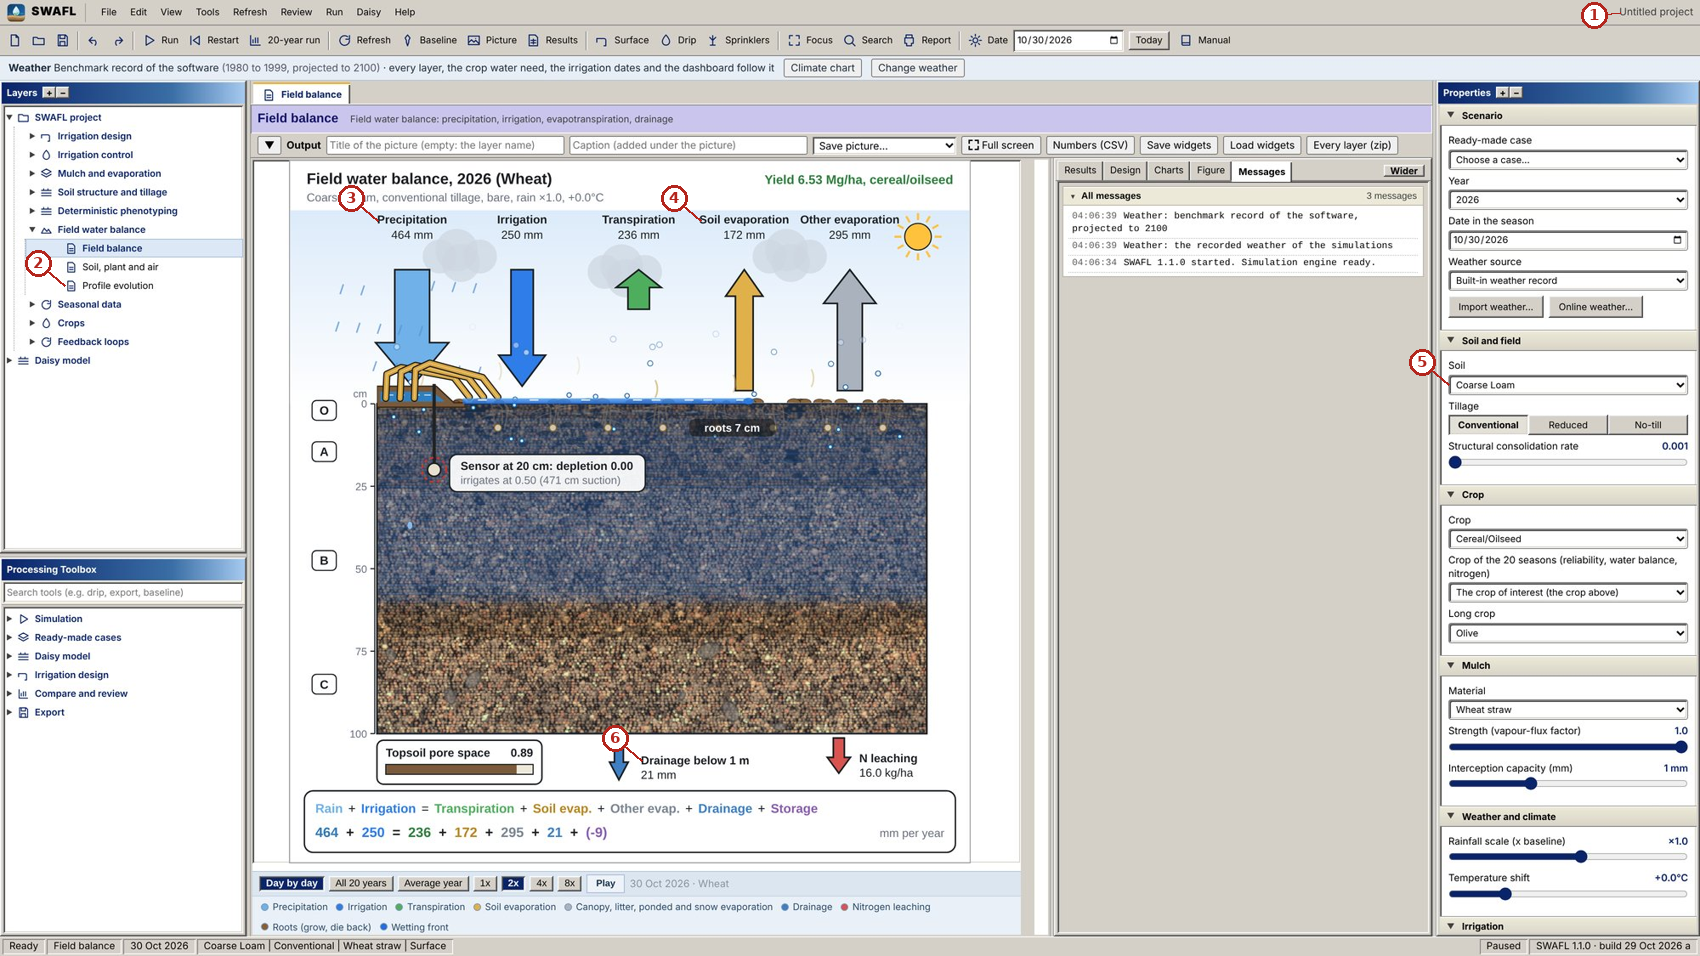
\includegraphics[width=\textwidth,height=0.42\textheight,keepaspectratio]{../figures/annot/p2_fig-shot-dash-messages_0.png}\end{center}

\textbf{What the numbered labels point to.}
\begin{enumerate}[nosep,label=\protect\circled{\arabic*}]
\item ``Untitled project'': a heading or control of this screen; the caption above says which layer it belongs to.
\item ``Profile evolution'': a heading or control of this screen; the caption above says which layer it belongs to.
\item ``Precipitation'': rain, from the weather of the project.
\item ``Soil evaporation'': evaporation from the soil (and, where stated, from mulch or canopy).
\item ``Coarse Loam v'': the soil of the project, which every layer uses.
\item ``Drainage below 1m'': rain, from the weather of the project.
\end{enumerate}

\textbf{What it shows.} SWAFL Desktop: dashboard messages. Panels: (a) Dashboard, messages tab: the decision messages and warnings of the current state.

\textbf{How to read the labels, symbols and colours.} A screen of the software as it appears to the user; the labelled areas are the inputs, the figure and the numbers of the layer named in the caption.

\textbf{What affects it, and why it happens.} Messages fire when a number crosses a threshold (stress, drainage, efficiency), so the user sees what to change. 

\textbf{How it is made.} Screen capture of SWAFL Desktop 1.1.0 (not regenerated).


\subsection{Derivation: Water balance of the column}\label{der:s2:1}
Mass conservation of the column between the surface and 1\,m gives $P+I=T+E+E_{\mathrm{oth}}+D+\Delta S$ per unit area, with all terms in mm; every engine is constructed so that this balance closes, and its residual is the test of Engine~2.


\subsection{Why it happens}
\paragraph{Why the meta-model ranks well but has an offset.} It is built from ratios of simulated outcomes, which preserve the order of the scenarios, while its absolute level is anchored to one reference run, so an error in the anchor shifts all values.

\section{Infiltration and surface irrigation}
Green--Ampt infiltration and the advance of water in a furrow.

\subsection{Contribution 5: a defect found and removed in surface irrigation}\label{con:s2:5}
\begin{problem}
The surface layer under-predicted slow advance (up to $-29\,\%$ in a published example). Why?
\end{problem}
\begin{keyresult}
\[\underbrace{x(t)}_{\circled{1}}=\frac{Qt}{\sigma_yA_0+\underbrace{\sigma_z(r)}_{\circled{2}}kt^Aw},\qquad \sigma_z=\frac{A+\underbrace{r}_{\circled{3}}(1-A)+1}{(1+A)(1+r)}\]
\end{keyresult}
\begin{pins}
\pin{1}{The advance distance at time $t$.}
\pin{2}{The subsurface shape factor depends on the advance exponent $r$.}
\pin{3}{The first release fixed $r$; for slow advance the true $r$ is smaller, $\sigma_z$ too small and the advance too short. Iterating $r$ with the computed advance removed the error, now within $-0.2$ to $+0.5\,\%$ of the published advance times.}
\end{pins}

\subsection{Worked numbers, part 4: infiltration (Green--Ampt)}
Water enters behind a sharp front. With $K_s$, front suction $\psi_f$ and water-content jump $\Delta\theta$, the infiltrated depth $F$ after time $t$ solves $F-\psi_f\Delta\theta\ln(1+F/(\psi_f\Delta\theta))=K_st$, found by trying values of $F$ until both sides agree.


\subsection{Worked numbers, part 5: surface irrigation advance}
The water admitted ($Q\,t$) is split between the surface and the soil; dividing by the volume per metre gives the advance $x(t)=Qt/(\sigma_yA_0+\sigma_zkt^Aw)$. The efficiencies follow from the stored, percolated and runoff volumes and add to one.


\subsection{Reading Figure 7 of the article}
\begin{center}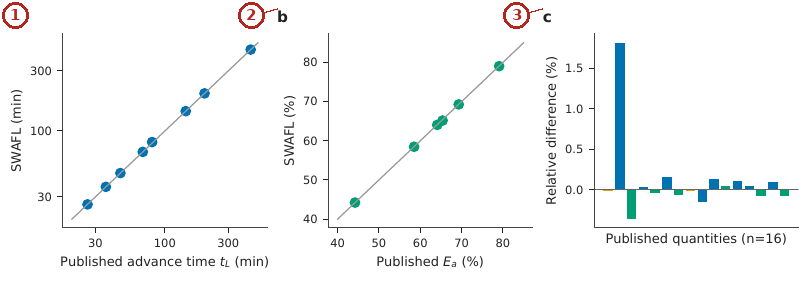
\includegraphics[width=\textwidth,height=0.42\textheight,keepaspectratio]{../figures/annot/p2_fig-ws_0.png}\end{center}

\textbf{What the numbered labels point to.}
\begin{enumerate}[nosep,label=\protect\circled{\arabic*}]
\item Panel (a): Advance time $t_L$. \emph{Why:} Points on the 1:1 line: the advance computed matches the published example.
\item Panel (b): application efficiency $E_a$ (published versus SWAFL; grey line is 1:1). \emph{Why:} Efficiencies match because they follow from the same volumes.
\item Panel (c): relative differences of the 16 quantities (blue: advance and required times; green: efficiencies). \emph{Why:} All 16 quantities lie within a few per cent, so the procedure is reproduced.
\end{enumerate}

\textbf{What it shows.} Verification against Example 6.1. (a) Advance time $t_L$, (b) application efficiency $E_a$ (published versus SWAFL; grey line is 1:1), (c) relative differences of the 16 quantities (blue: advance and required times; green: efficiencies).

\textbf{How to read the labels, symbols and colours.} (a) Advance time and (b) efficiency, published against SWAFL with the 1:1 line; (c) relative differences of 16 quantities.

\textbf{What affects it, and why it happens.} Points on the 1:1 line show the implementation reproduces the published worked example.

\textbf{How it is made.} Figure drawn by the script from the input data. Script: \nolinkurl{Manuscripts/reproducibility/analysis/p3_figs.py}. Input: \nolinkurl{Data/daisy_ensemble.csv.gz}.


\subsection{Reading Figure 11 of the article}
\begin{center}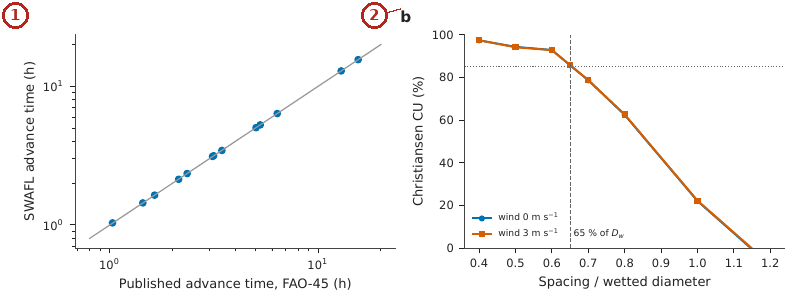
\includegraphics[width=\textwidth,height=0.42\textheight,keepaspectratio]{../figures/annot/p2_fig-lit_0.png}\end{center}

\textbf{What the numbered labels point to.}
\begin{enumerate}[nosep,label=\protect\circled{\arabic*}]
\item Panel (a): Thirteen advance times of the FAO Irrigation Paper~45 border examples (published against SWAFL; grey line 1:1). \emph{Why:} Points on the 1:1 line: the shipped layer reproduces published advance times.
\item Panel (b): Christiansen coefficient of uniformity of the impact-sprinkler layer against spacing as a share of the wetted diameter, without wind and at 3\,m\,s$^{-1}$; dashed: 65\,\% spacing rule, dotted: CU of 85\,\%. \emph{Why:} Uniformity falls when sprinklers are spaced beyond about 65\,\% of the wetted diameter because the patterns overlap too little; wind makes it worse.
\end{enumerate}

\textbf{What it shows.} Checks against published sources. (a) Thirteen advance times of the FAO Irrigation Paper~45 border examples (published against SWAFL; grey line 1:1). (b) Christiansen coefficient of uniformity of the impact-sprinkler layer against spacing as a share of the wetted diameter, without wind and at 3\,m\,s$^{-1}$; dashed: 65\,\% spacing rule, dotted: CU of 85\,\%.

\textbf{How to read the labels, symbols and colours.} (a) Thirteen published advance times against SWAFL, 1:1 line; (b) uniformity against spacing, without and with wind.

\textbf{What affects it, and why it happens.} Uniformity falls as spacing exceeds about 65\,\% of the wetted diameter because the overlap of patterns becomes too small.

\textbf{How it is made.} Figure drawn by the script from the input data. Script: \nolinkurl{Manuscripts/reproducibility/analysis/p3_lit_figs.py}. Input: \nolinkurl{Data/daisy_ensemble.csv.gz}.


\subsection{Reading Figure 21 of the article}
\begin{center}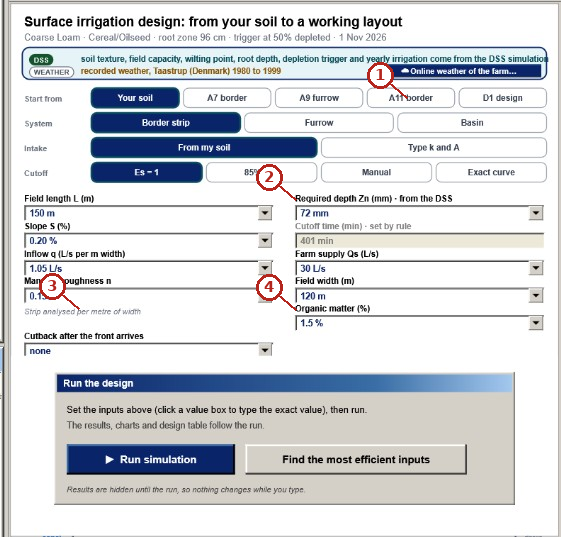
\includegraphics[width=\textwidth,height=0.42\textheight,keepaspectratio]{../figures/annot/p2_fig-shot-layer-sid_0.png}\end{center}

\textbf{What the numbered labels point to (picture 1 of 2: Surface-irrigation layer: start from your soil or a textbook design (A7, A9, A11, D1), border strip, furrow or basin, intake from the soil or by $k$ and $A$, the cutoff rule, and the inputs carried from the soil, root zone and trigger of the DSS (Section~Section~4.4 of the article)).}
\begin{enumerate}[nosep,label=\protect\circled{\arabic*}]
\item ``border'': a heading or control of this screen; the caption above says which layer it belongs to.
\item ``Required depth Zn from the DSS'': a heading or control of this screen; the caption above says which layer it belongs to.
\item ``per metre'': a heading or control of this screen; the caption above says which layer it belongs to.
\item ``Organic matter (\%)'': a heading or control of this screen; the caption above says which layer it belongs to.
\end{enumerate}

\begin{center}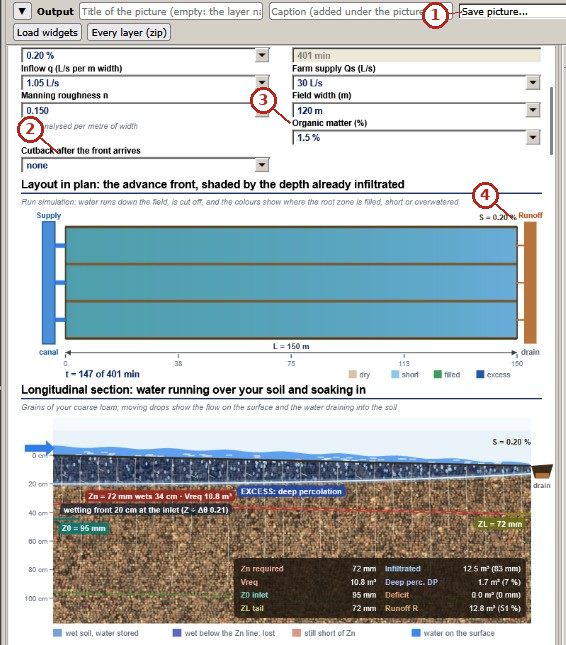
\includegraphics[width=\textwidth,height=0.42\textheight,keepaspectratio]{../figures/annot/p2_fig-shot-layer-sid_1.png}\end{center}

\textbf{What the numbered labels point to (picture 2 of 2: Surface irrigation: layout in plan with the advance front shaded by the depth already infiltrated, and the longitudinal section with the wetting front, the required depth $Z_n$, deep percolation and runoff (Eq.~(46) and Eq.~(47) of the article)).}
\begin{enumerate}[nosep,label=\protect\circled{\arabic*}]
\item ``Save picture'': a heading or control of this screen; the caption above says which layer it belongs to.
\item ``after the front arrives'': a heading or control of this screen; the caption above says which layer it belongs to.
\item ``Organic matter'': a heading or control of this screen; the caption above says which layer it belongs to.
\item ``Runoff'': a heading or control of this screen; the caption above says which layer it belongs to.
\end{enumerate}

\textbf{What it shows.} SWAFL Desktop: surface irrigation. Panels: (a) Surface-irrigation layer: start from your soil or a textbook design (A7, A9, A11, D1), border strip, furrow or basin, intake from the soil or by $k$ and $A$, the cutoff rule, and the inputs carried from the soil, root zone and trigger of the DSS (Section~Section~4.4 of the article). (b) Surface irrigation: layout in plan with the advance front shaded by the depth already infiltrated, and the longitudinal section with the wetting front, the required depth $Z_n$, deep percolation and runoff (Eq.~(46) and Eq.~(47) of the article).

\textbf{How to read the labels, symbols and colours.} A screen of the software as it appears to the user; the labelled areas are the inputs, the figure and the numbers of the layer named in the caption.

\textbf{What affects it, and why it happens.} Water advances down the field while it infiltrates; the far end receives less, so the cutoff time sets the balance between shortfall and deep percolation. 

\textbf{How it is made.} Screen capture of SWAFL Desktop 1.1.0 (not regenerated).


\subsection{Reading Figure 22 of the article}
\begin{center}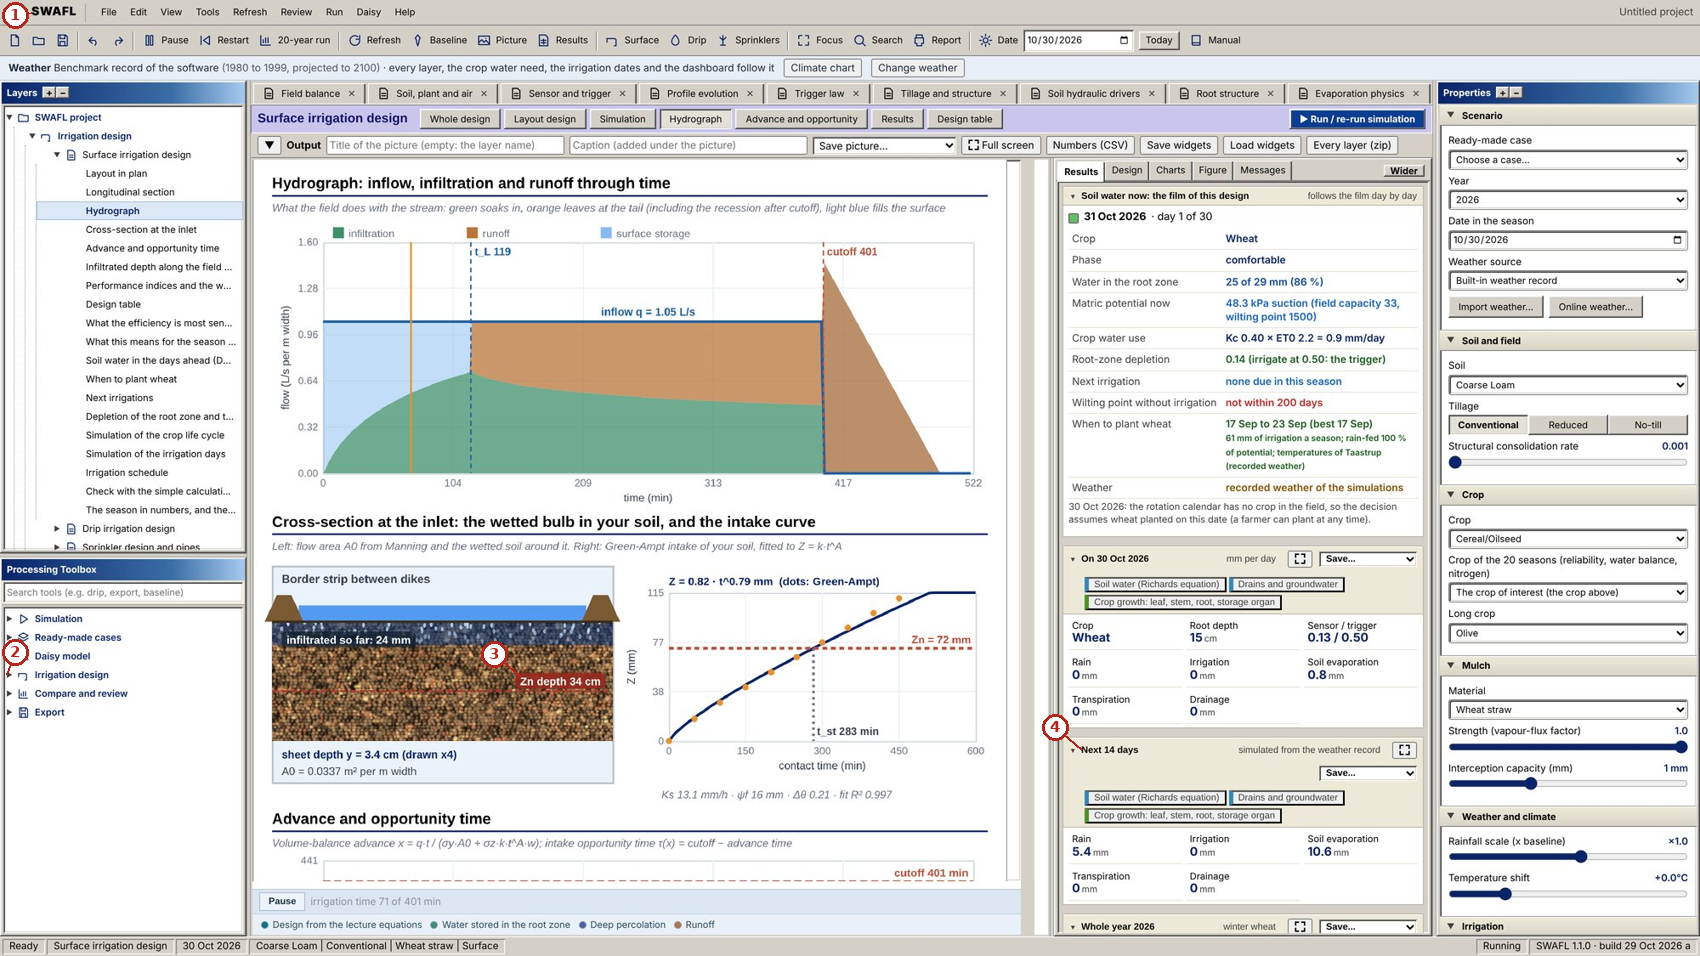
\includegraphics[width=\textwidth,height=0.42\textheight,keepaspectratio]{../figures/annot/p2_fig-shot-sid-sec-sched_0.png}\end{center}

\textbf{What the numbered labels point to (picture 1 of 2: Surface irrigation: hydrograph of inflow, infiltration and runoff through time.).}
\begin{enumerate}[nosep,label=\protect\circled{\arabic*}]
\item ``SWAFL View Run Daisy Help'': the menu bar of the program (file, view, run, Daisy, help).
\item ``design'': a heading or control of this screen; the caption above says which layer it belongs to.
\item ``Zn depth 34m'': a heading or control of this screen; the caption above says which layer it belongs to.
\item ``Next 14 days'': the decision for the next 14 days, from the soil water of the day.
\end{enumerate}

\begin{center}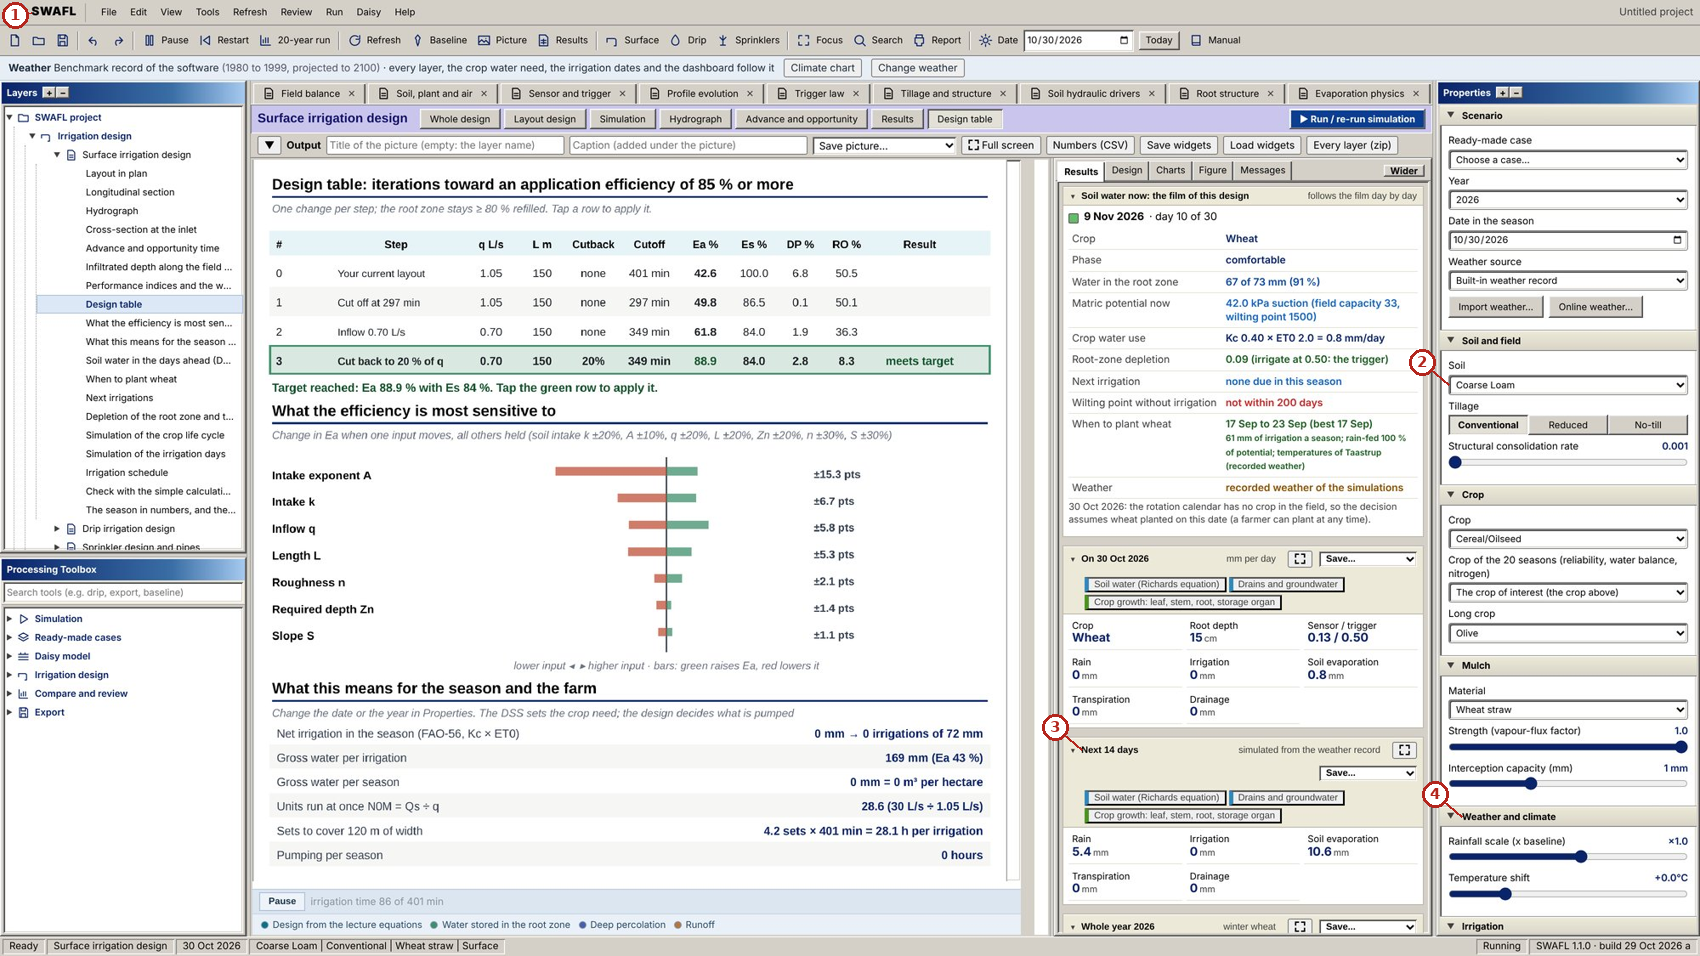
\includegraphics[width=\textwidth,height=0.42\textheight,keepaspectratio]{../figures/annot/p2_fig-shot-sid-sec-sched_1.png}\end{center}

\textbf{What the numbered labels point to (picture 2 of 2: Surface irrigation: design table of options with application and storage efficiency, deep percolation and runoff (Eq.~(48) of the article).).}
\begin{enumerate}[nosep,label=\protect\circled{\arabic*}]
\item ``SWAFL View Run Daisy Help'': the menu bar of the program (file, view, run, Daisy, help).
\item ``Coarse Loam'': the soil of the project, which every layer uses.
\item ``Next 14 days'': the decision for the next 14 days, from the soil water of the day.
\item ``Weather and climate'': the weather of the project: built-in record, a file of the user or online weather of any place.
\end{enumerate}

\textbf{What it shows.} SWAFL Desktop: surface irrigation, schedule and design table. Panels: (a) Surface irrigation: hydrograph of inflow, infiltration and runoff through time. (b) Surface irrigation: design table of options with application and storage efficiency, deep percolation and runoff (Eq.~(48) of the article).

\textbf{How to read the labels, symbols and colours.} A screen of the software as it appears to the user; the labelled areas are the inputs, the figure and the numbers of the layer named in the caption.

\textbf{What affects it, and why it happens.} The schedule repeats irrigation when the root zone is depleted to the trigger; the design table shows the volumes and efficiencies of each event. 

\textbf{How it is made.} Screen capture of SWAFL Desktop 1.1.0 (not regenerated).


\subsection{Derivation: Green--Ampt infiltration}\label{der:s2:9}
Behind a sharp wetting front at depth $L_f$ with uniform water-content jump $\Delta\theta$ and front suction $\psi_f$, Darcy's law gives the infiltration rate $f=K_s(L_f+\psi_f)/L_f$ (ponding head neglected). With $F=L_f\Delta\theta$, $f=\dd F/\dd t=K_s(1+\psi_f\Delta\theta/F)$. Separating variables and integrating from $F=0$ at $t=0$:
\begin{equation}F-\psi_f\Delta\theta\ln\Bigl(1+\frac{F}{\psi_f\Delta\theta}\Bigr)=K_st.\end{equation}


\subsection{Derivation: Surface irrigation: volume balance and advance}\label{der:s2:10}
At time $t$ after the start, the volume admitted, $Qt$, is stored on the surface (mean flow area $\sigma_yA_0$ over the advance length $x$) and in the soil (mean infiltrated depth $\sigma_zZ(t)$ over the wetted width $w$): $Qt=\sigma_yA_0x+\sigma_zkt^{A}wx$, so $x(t)=Qt/(\sigma_yA_0+\sigma_zkt^{A}w)$. If the advance follows a power law $x\propto t^{r}$ and the intake opportunity time at distance $s$ is $t-t_x(s)$, the mean of $Z$ along the advance is $Z(t)$ times
\begin{equation}\sigma_z=\int_0^1(1-\xi^{1/r})^{A}\dd\xi\;\simeq\;\frac{A+r(1-A)+1}{(1+A)(1+r)},\end{equation}where the right-hand side is the closed approximation used in surface-irrigation practice \citep{Walker1987}; it is exact for $A=0$ and $A=1$.
The volumes applied, required, infiltrated, stored, percolated and run off satisfy $V_{\mathrm{app}}=V_{\mathrm{inf}}+V_{\mathrm{ro}}$ and $V_{\mathrm{inf}}=V_{\mathrm{st}}+V_{\mathrm{dp}}$, so the application efficiency, deep percolation and runoff fractions add to one.


\section{Drip and sprinkler irrigation}
Friction in a lateral, uniformity and nozzle discharge.

\subsection{Worked numbers, part 6: friction in a drip lateral}
The Hazen--Williams loss of the full flow is reduced by the Christiansen factor because the flow falls along the lateral. \emph{Example:} 50 outlets give $F_c=1/2.852+1/100+\sqrt{0.852}/15\,000=0.361$; a 100\,m lateral of 16\,mm with 0.5\,L\,s$^{-1}$ at the inlet loses about 17.6\,m.


\subsection{Worked numbers, part 7: a sprinkler nozzle}
$q=0.95A_n\sqrt{2gh_n}$. \emph{Example:} a 4\,mm nozzle at 30\,m head: $A_n=1.26\times10^{-5}$\,m$^2$, $\sqrt{2\times9.81\times30}=24.3$\,m\,s$^{-1}$, $q=2.9\times10^{-4}$\,m$^3$\,s$^{-1}=17.4$\,L\,min$^{-1}$.


\subsection{Reading Figure 10 of the article}
\begin{center}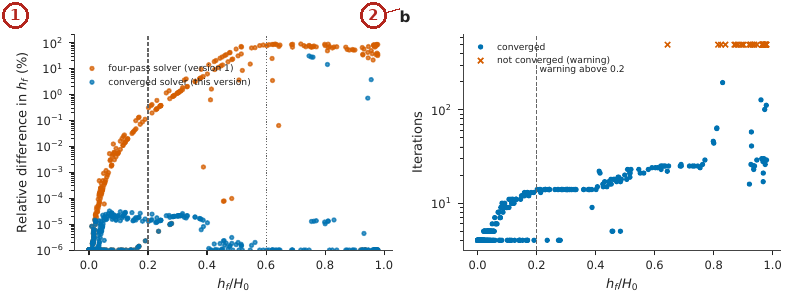
\includegraphics[width=\textwidth,height=0.42\textheight,keepaspectratio]{../figures/annot/p2_fig-drip_0.png}\end{center}

\textbf{What the numbered labels point to.}
\begin{enumerate}[nosep,label=\protect\circled{\arabic*}]
\item Panel (a): Relative difference in total head loss for the four-pass solver of version~1 and the converged solver, against the loss ratio $h_f/H_0$ (dashed: design limit 0.2; dotted: 0.6). \emph{Why:} When friction is a large share of the head, emitter flows and heads are strongly coupled, so a few passes are not enough; the converged solver removes the error.
\item Panel (b): number of iterations of the converged solver; crosses mark configurations that did not converge. \emph{Why:} More iterations are needed as the coupling grows.
\end{enumerate}

\textbf{What it shows.} Drip-lateral solver versus an independent converged solver (400 random configurations). (a) Relative difference in total head loss for the four-pass solver of version~1 and the converged solver, against the loss ratio $h_f/H_0$ (dashed: design limit 0.2; dotted: 0.6); (b) number of iterations of the converged solver; crosses mark configurations that did not converge.

\textbf{How to read the labels, symbols and colours.} (a) Relative error of the lateral loss against the loss ratio, old and converged solver; dashed design limit 0.2; (b) iterations, crosses non-converged.

\textbf{What affects it, and why it happens.} Errors grow with the loss ratio because emitter flows and heads become strongly coupled; iterating to convergence removes them up to a large loss.

\textbf{How it is made.} Figure drawn by the script from the input data. Script: \nolinkurl{Manuscripts/reproducibility/analysis/p3_figs.py}. Input: \nolinkurl{Data/daisy_ensemble.csv.gz}.


\subsection{Reading Figure 23 of the article}
\begin{center}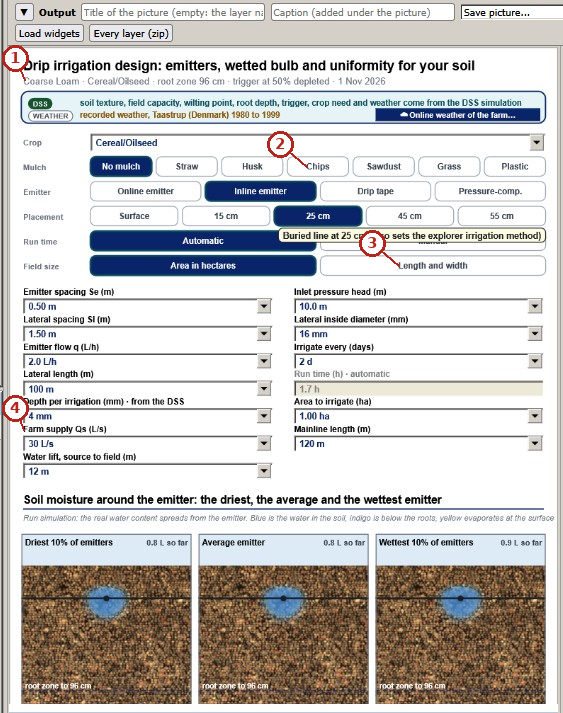
\includegraphics[width=\textwidth,height=0.42\textheight,keepaspectratio]{../figures/annot/p2_fig-shot-layer-drip_0.png}\end{center}

\textbf{What the numbered labels point to (picture 1 of 2: Drip-irrigation layer: crop, mulch, emitter type and placement, the design inputs, and the soil moisture around the driest, the average and the wettest emitter (Section~Section~4.4 of the article)).}
\begin{enumerate}[nosep,label=\protect\circled{\arabic*}]
\item ``Coarse Loam - Cereal'': the soil of the project, which every layer uses.
\item ``Chips'': a heading or control of this screen; the caption above says which layer it belongs to.
\item ``Length and width'': a heading or control of this screen; the caption above says which layer it belongs to.
\item ``Farm supply Qs'': a heading or control of this screen; the caption above says which layer it belongs to.
\end{enumerate}

\begin{center}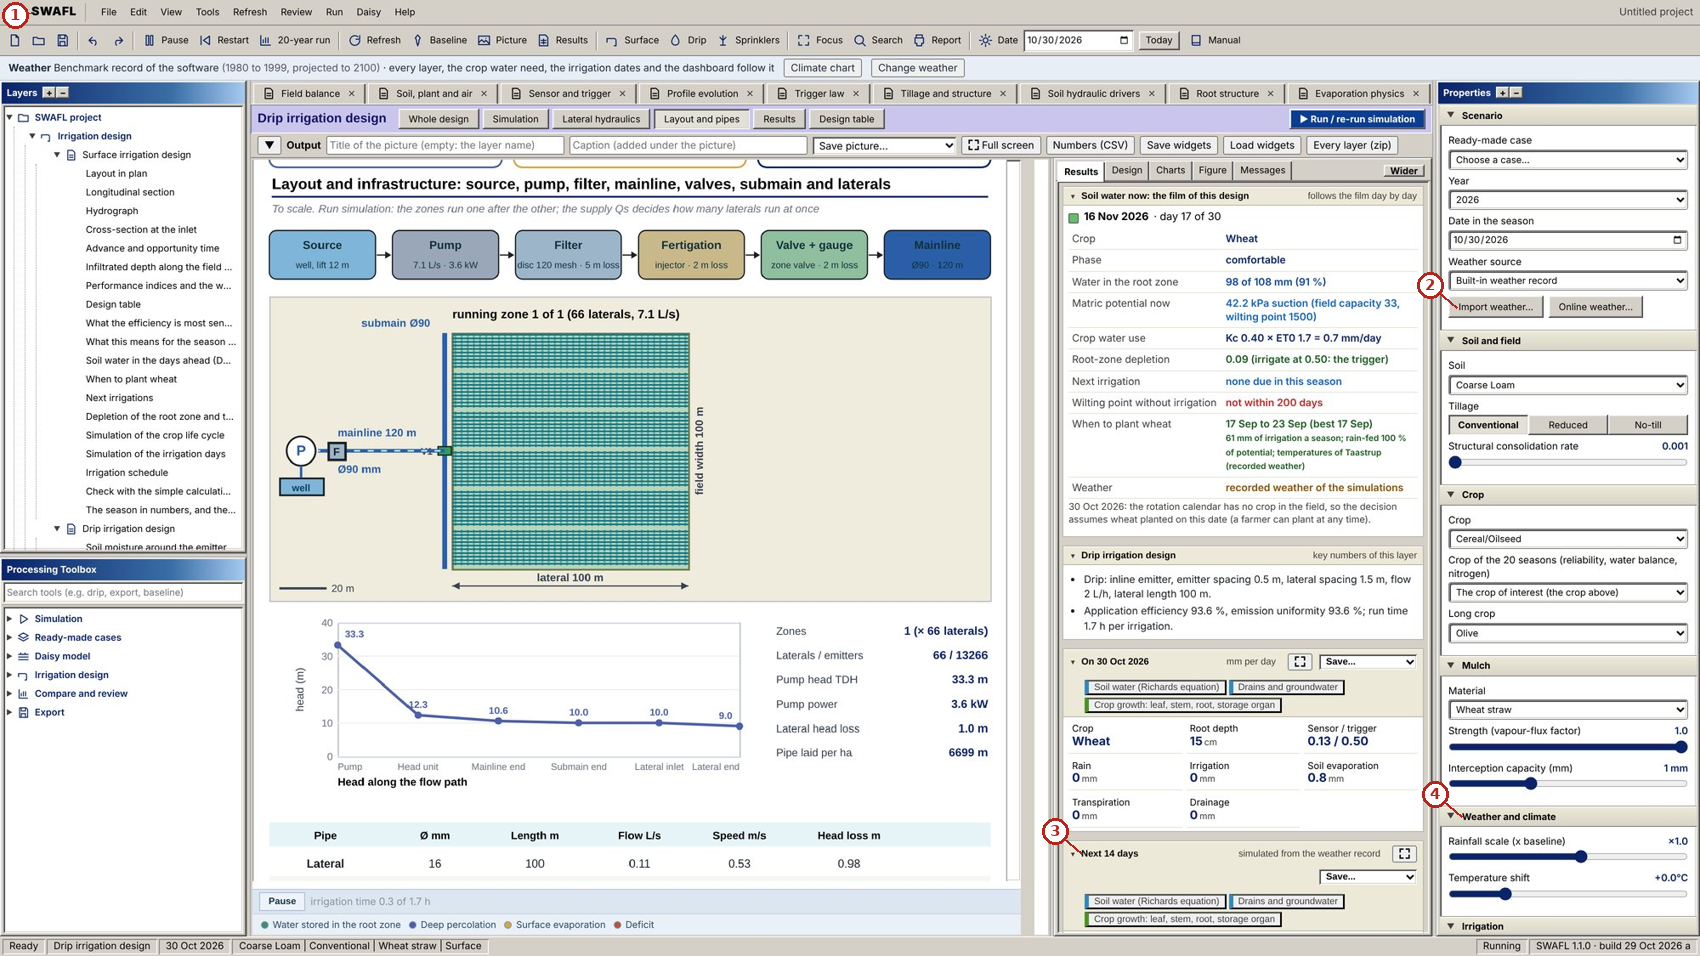
\includegraphics[width=\textwidth,height=0.42\textheight,keepaspectratio]{../figures/annot/p2_fig-shot-layer-drip_1.png}\end{center}

\textbf{What the numbered labels point to (picture 2 of 2: Drip irrigation: field layout and infrastructure.).}
\begin{enumerate}[nosep,label=\protect\circled{\arabic*}]
\item ``SWAFL View Run Daisy Help'': the menu bar of the program (file, view, run, Daisy, help).
\item ``Import weather... Online weather'': the weather of the project: built-in record, a file of the user or online weather of any place.
\item ``Next 14 days'': the decision for the next 14 days, from the soil water of the day.
\item ``Weather and climate'': the weather of the project: built-in record, a file of the user or online weather of any place.
\end{enumerate}

\textbf{What it shows.} SWAFL Desktop: drip irrigation. Panels: (a) Drip-irrigation layer: crop, mulch, emitter type and placement, the design inputs, and the soil moisture around the driest, the average and the wettest emitter (Section~Section~4.4 of the article). (b) Drip irrigation: field layout and infrastructure.

\textbf{How to read the labels, symbols and colours.} A screen of the software as it appears to the user; the labelled areas are the inputs, the figure and the numbers of the layer named in the caption.

\textbf{What affects it, and why it happens.} Water spreads from each emitter as a bulb whose size depends on the soil; friction along the lateral lowers the flow of distant emitters. 

\textbf{How it is made.} Screen capture of SWAFL Desktop 1.1.0 (not regenerated).


\subsection{Reading Figure 24 of the article}
\begin{center}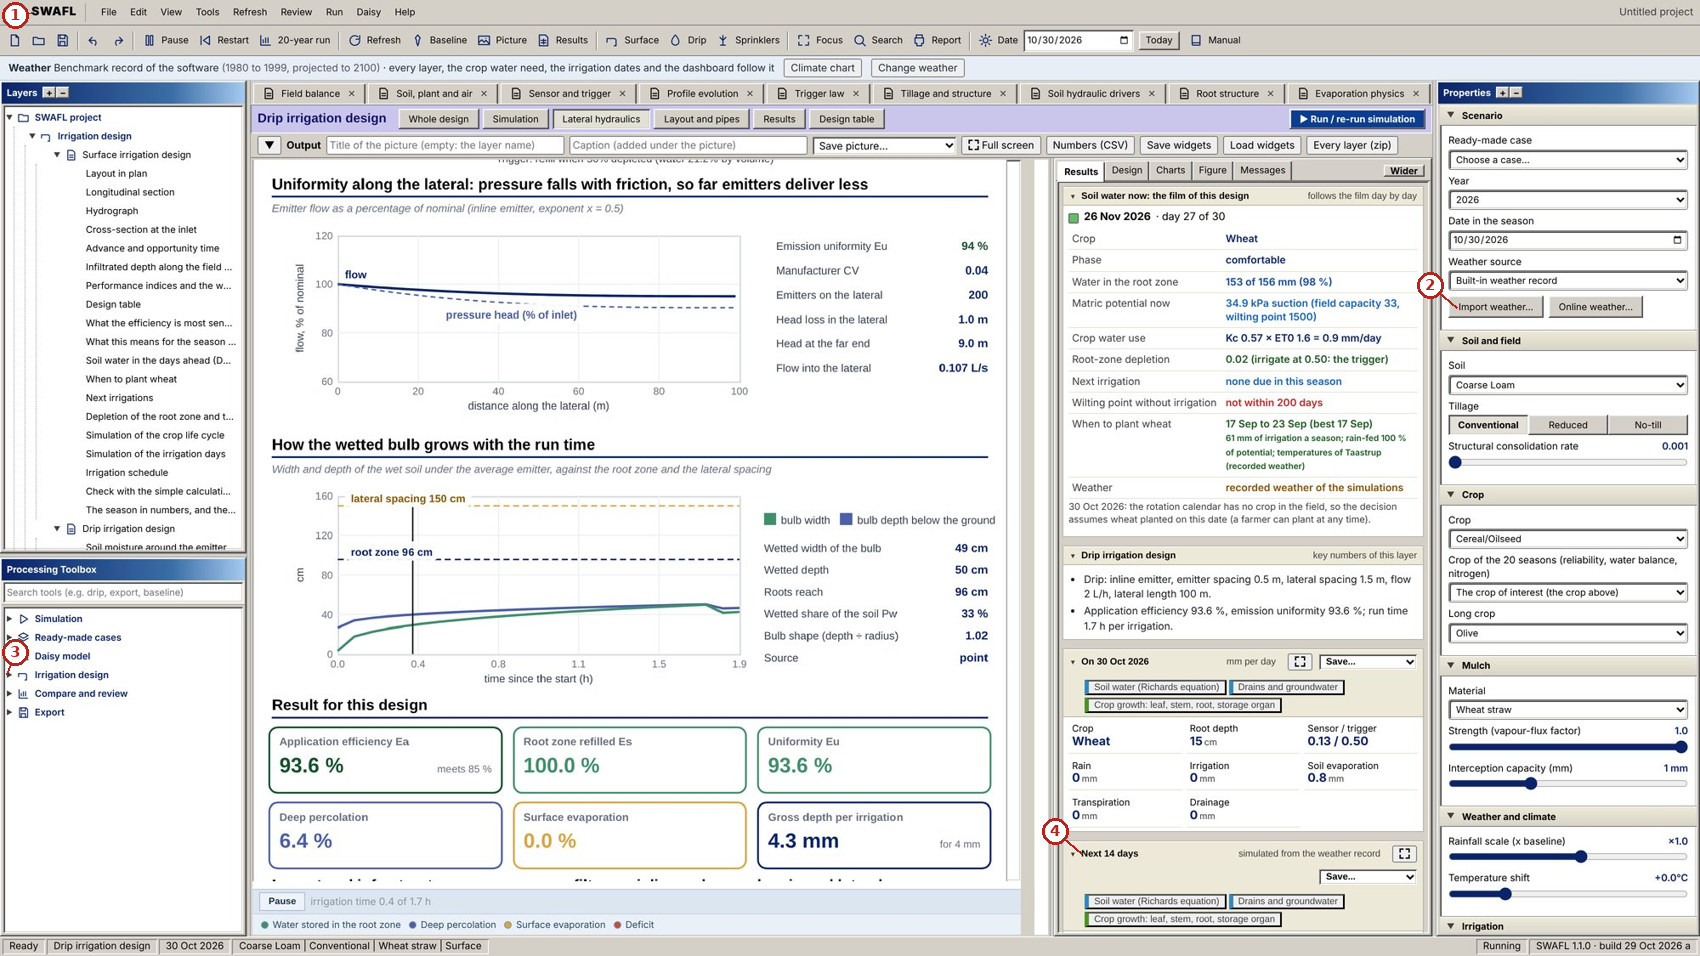
\includegraphics[width=\textwidth,height=0.42\textheight,keepaspectratio]{../figures/annot/p2_fig-shot-drip-sec-lateral_0.png}\end{center}

\textbf{What the numbered labels point to (picture 1 of 2: Drip irrigation: head and emitter flow along the lateral (Eq.~(49) of the article) with the 20\,\% loss warning.).}
\begin{enumerate}[nosep,label=\protect\circled{\arabic*}]
\item ``SWAFL View Run Daisy Help'': the menu bar of the program (file, view, run, Daisy, help).
\item ``Import weather... Online weather'': the weather of the project: built-in record, a file of the user or online weather of any place.
\item ``design'': a heading or control of this screen; the caption above says which layer it belongs to.
\item ``Next 14 days'': the decision for the next 14 days, from the soil water of the day.
\end{enumerate}

\begin{center}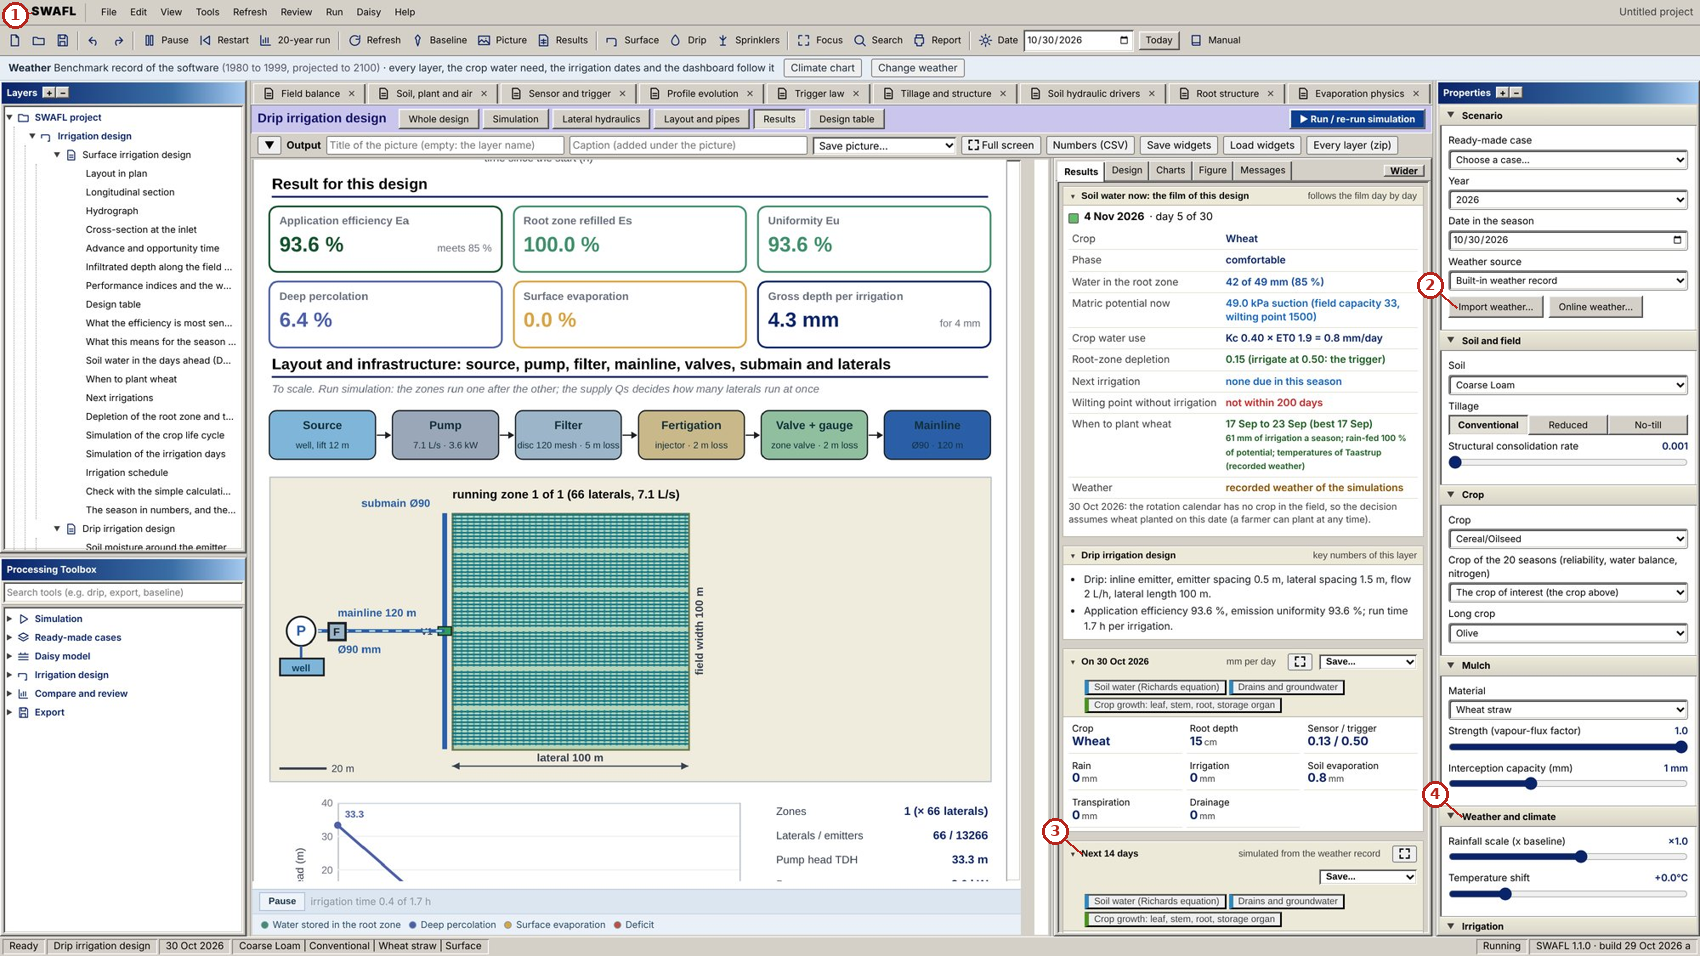
\includegraphics[width=\textwidth,height=0.42\textheight,keepaspectratio]{../figures/annot/p2_fig-shot-drip-sec-lateral_1.png}\end{center}

\textbf{What the numbered labels point to (picture 2 of 2: Drip irrigation: result summary with emission uniformity (Eq.~(50) of the article) and efficiencies.).}
\begin{enumerate}[nosep,label=\protect\circled{\arabic*}]
\item ``SWAFL View Run Daisy Help'': the menu bar of the program (file, view, run, Daisy, help).
\item ``Import weather... Online weather'': the weather of the project: built-in record, a file of the user or online weather of any place.
\item ``Next 14 days'': the decision for the next 14 days, from the soil water of the day.
\item ``Weather and climate'': the weather of the project: built-in record, a file of the user or online weather of any place.
\end{enumerate}

\textbf{What it shows.} SWAFL Desktop: drip irrigation, lateral and results. Panels: (a) Drip irrigation: head and emitter flow along the lateral (Eq.~(49) of the article) with the 20\,\% loss warning. (b) Drip irrigation: result summary with emission uniformity (Eq.~(50) of the article) and efficiencies.

\textbf{How to read the labels, symbols and colours.} A screen of the software as it appears to the user; the labelled areas are the inputs, the figure and the numbers of the layer named in the caption.

\textbf{What affects it, and why it happens.} Head falls along the lateral by friction, so emitter flow falls; the design keeps the loss within the limit. 

\textbf{How it is made.} Screen capture of SWAFL Desktop 1.1.0 (not regenerated).


\subsection{Reading Figure 25 of the article}
\begin{center}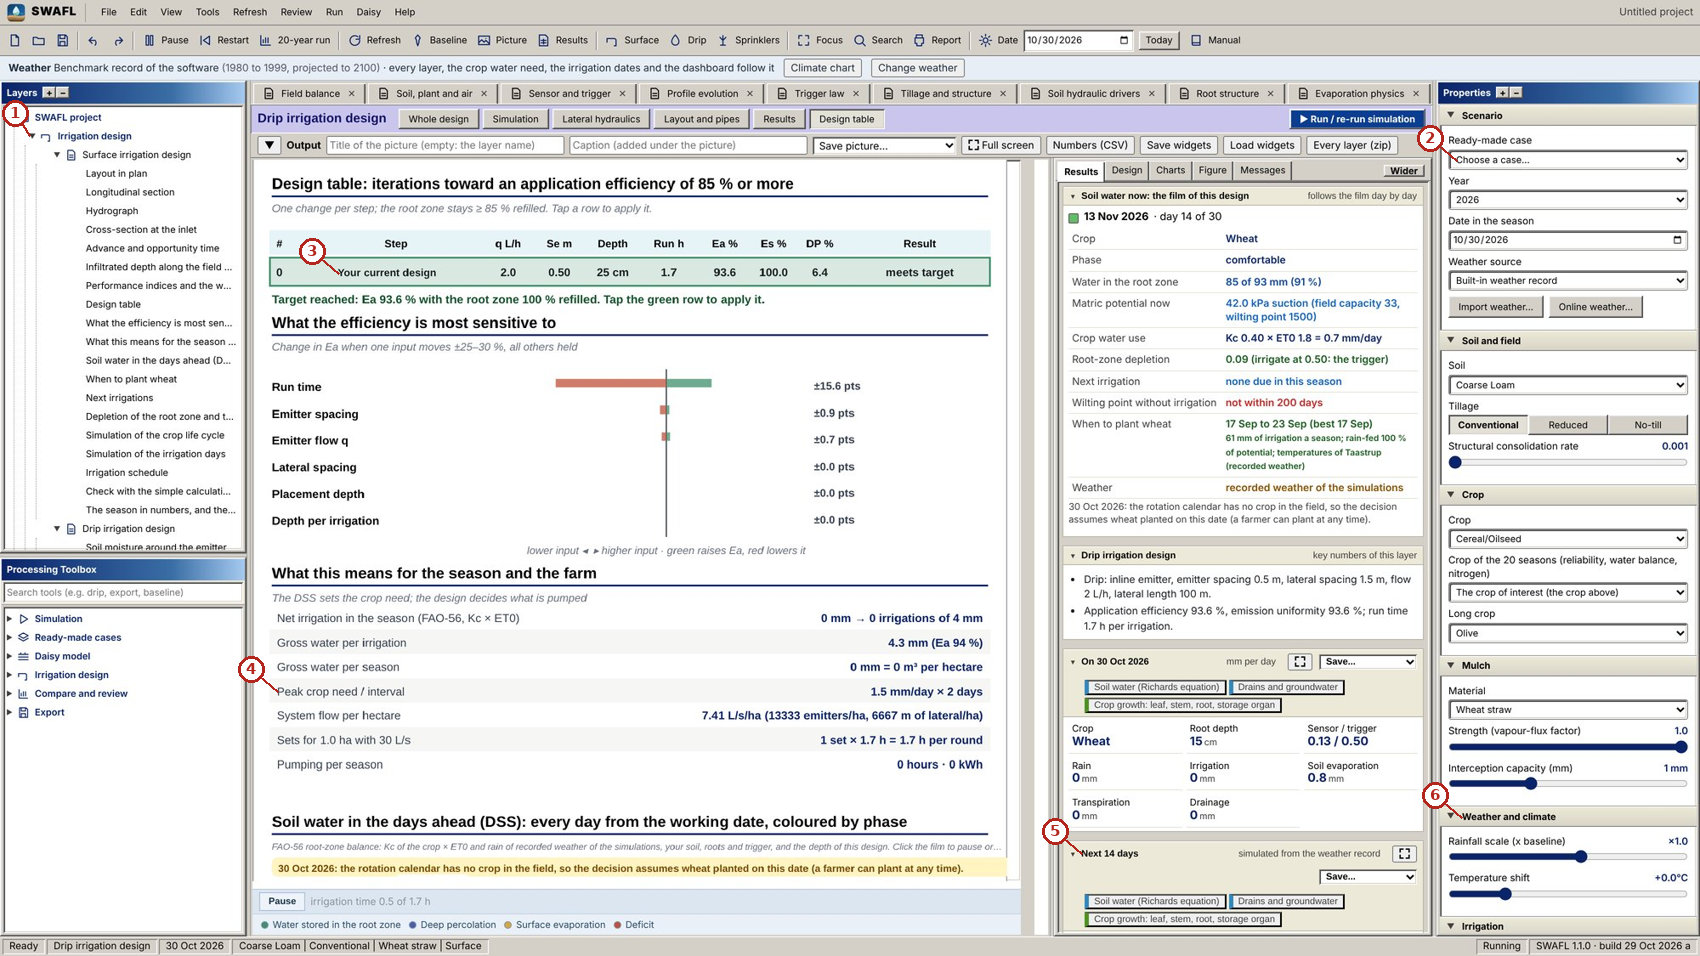
\includegraphics[width=\textwidth,height=0.42\textheight,keepaspectratio]{../figures/annot/p2_fig-shot-drip-sec-table_0.png}\end{center}

\textbf{What the numbered labels point to.}
\begin{enumerate}[nosep,label=\protect\circled{\arabic*}]
\item ``Irrigation design'': the irrigation-design group of the Layers tree and its layers.
\item ``Choose a case'': the ready-made cases of the Properties panel.
\item ``Your current design'': a heading or control of this screen; the caption above says which layer it belongs to.
\item ``Peak crop need / interval'': the crop of the project and its stage.
\item ``Next 14 days'': the decision for the next 14 days, from the soil water of the day.
\item ``Weather and climate'': the weather of the project: built-in record, a file of the user or online weather of any place.
\end{enumerate}

\textbf{What it shows.} SWAFL Desktop: drip irrigation, design table. Panels: (a) Drip irrigation: design table, iterations toward an application efficiency of 85\,\% or more.

\textbf{How to read the labels, symbols and colours.} A screen of the software as it appears to the user; the labelled areas are the inputs, the figure and the numbers of the layer named in the caption.

\textbf{What affects it, and why it happens.} The design iterates spacing and run time until the application efficiency and uniformity meet their targets. 

\textbf{How it is made.} Screen capture of SWAFL Desktop 1.1.0 (not regenerated).


\subsection{Reading Figure 26 of the article}
\begin{center}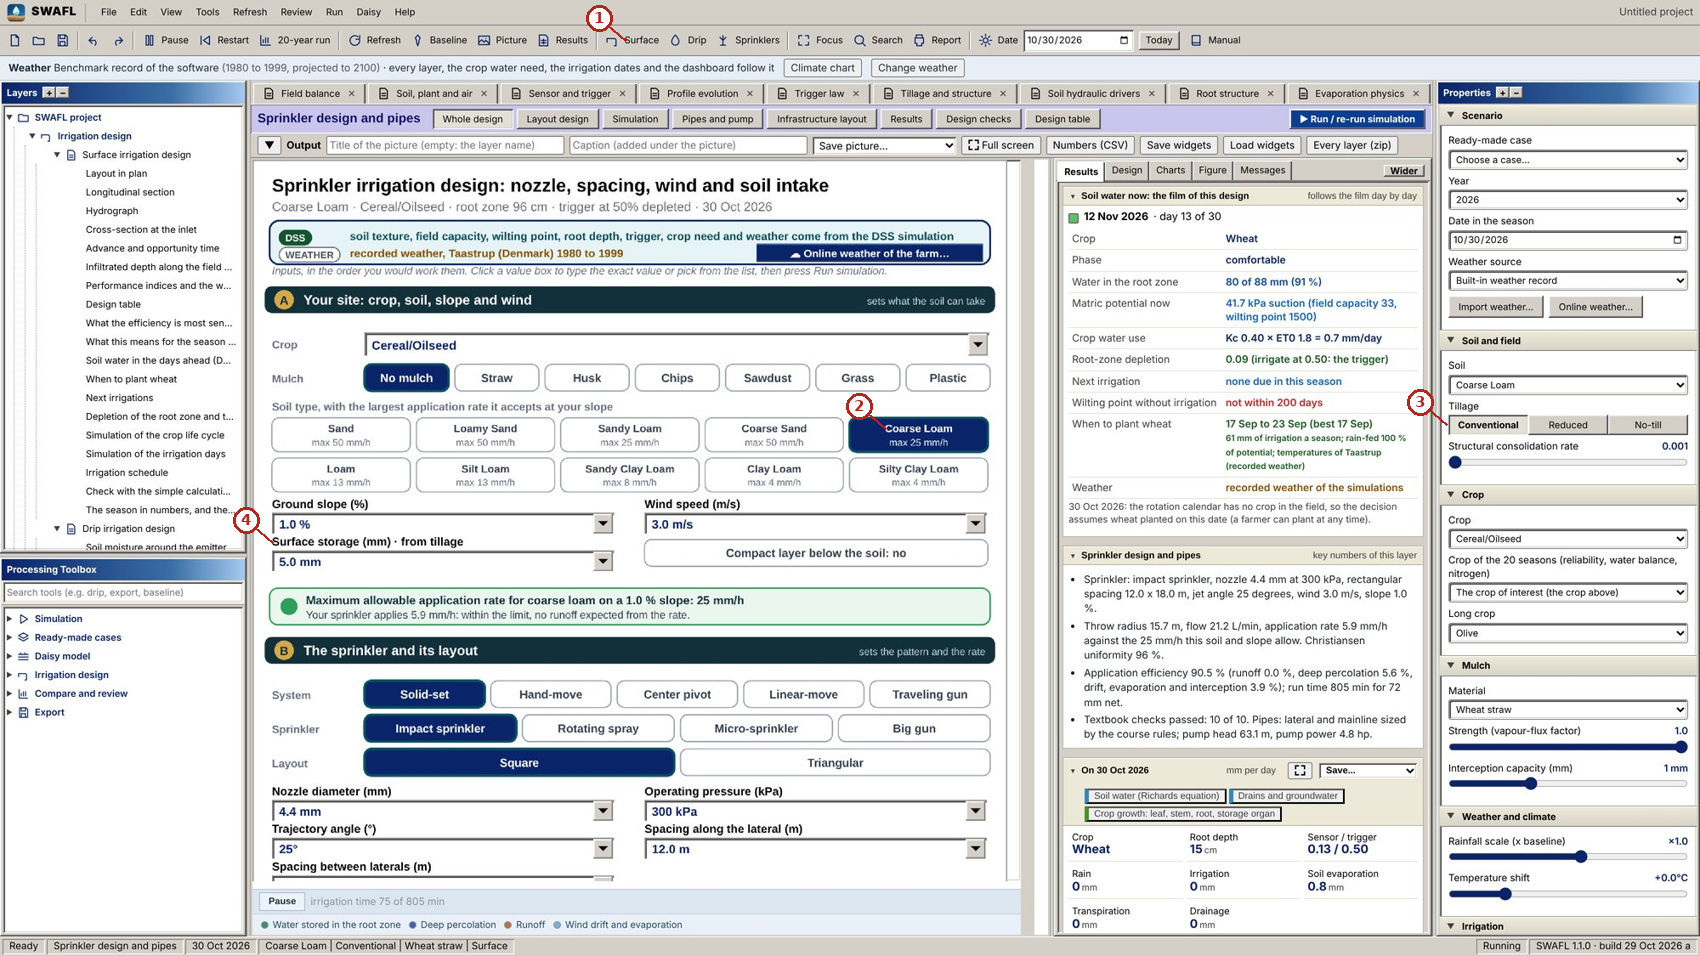
\includegraphics[width=\textwidth,height=0.42\textheight,keepaspectratio]{../figures/annot/p2_fig-shot-layer-spr_0.png}\end{center}

\textbf{What the numbered labels point to (picture 1 of 2: Sprinkler layer: nozzle, wetted radius, pattern, overlap and uniformity (Eq.~(51) of the article; Section~Section~4.4 of the article).).}
\begin{enumerate}[nosep,label=\protect\circled{\arabic*}]
\item ``Surface © Sprinklers'': the irrigation-design group of the Layers tree and its layers.
\item ``Coarse Lo'': a heading or control of this screen; the caption above says which layer it belongs to.
\item ``Reduced No-till'': a heading or control of this screen; the caption above says which layer it belongs to.
\item ``Surface storage (mm) - from tillage'': a heading or control of this screen; the caption above says which layer it belongs to.
\end{enumerate}

\begin{center}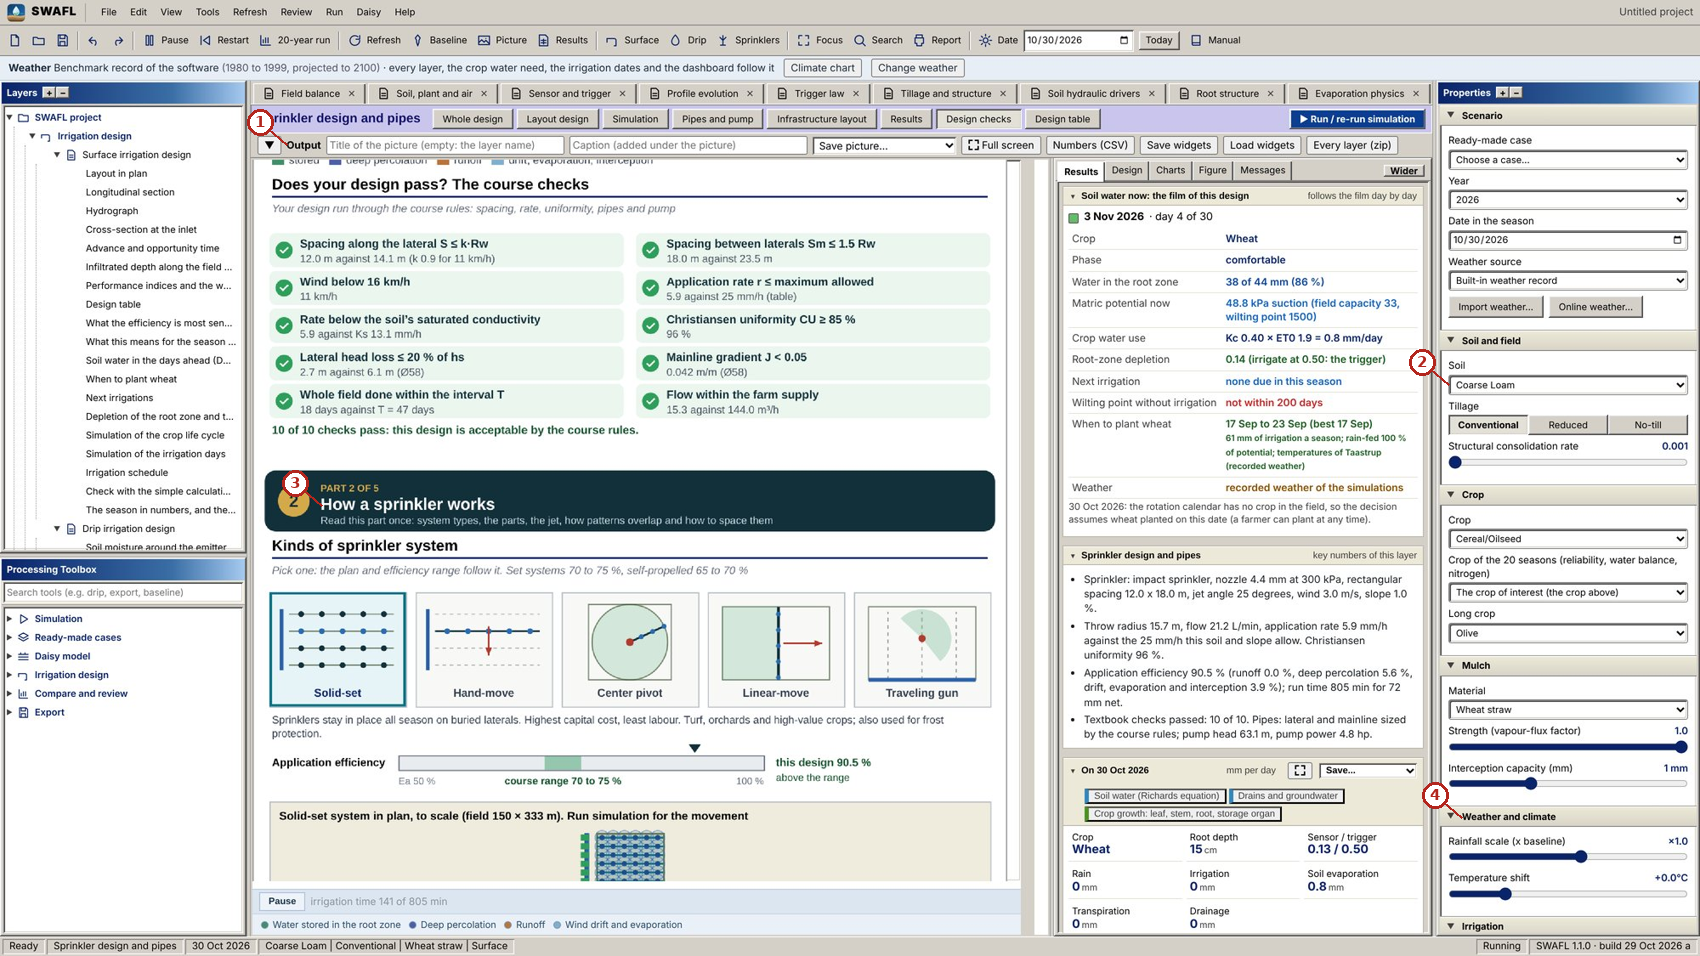
\includegraphics[width=\textwidth,height=0.42\textheight,keepaspectratio]{../figures/annot/p2_fig-shot-layer-spr_1.png}\end{center}

\textbf{What the numbered labels point to (picture 2 of 2: Sprinkler design: textbook decision checklist (sprinkler class, spacing, application rate, sets per day).).}
\begin{enumerate}[nosep,label=\protect\circled{\arabic*}]
\item ``Output'': the output bar of the layer: title and caption of the picture, save the picture, full screen, numbers as CSV.
\item ``Coarse Loam v'': the soil of the project, which every layer uses.
\item ``How a sprinkler works'': a heading or control of this screen; the caption above says which layer it belongs to.
\item ``Weather and climate'': the weather of the project: built-in record, a file of the user or online weather of any place.
\end{enumerate}

\textbf{What it shows.} SWAFL Desktop: sprinkler irrigation. Panels: (a) Sprinkler layer: nozzle, wetted radius, pattern, overlap and uniformity (Eq.~(51) of the article; Section~Section~4.4 of the article). (b) Sprinkler design: textbook decision checklist (sprinkler class, spacing, application rate, sets per day).

\textbf{How to read the labels, symbols and colours.} A screen of the software as it appears to the user; the labelled areas are the inputs, the figure and the numbers of the layer named in the caption.

\textbf{What affects it, and why it happens.} Each sprinkler wets a circle that is wettest near the nozzle; overlap of neighbouring circles evens out the depth. 

\textbf{How it is made.} Screen capture of SWAFL Desktop 1.1.0 (not regenerated).


\subsection{Reading Figure 27 of the article}
\begin{center}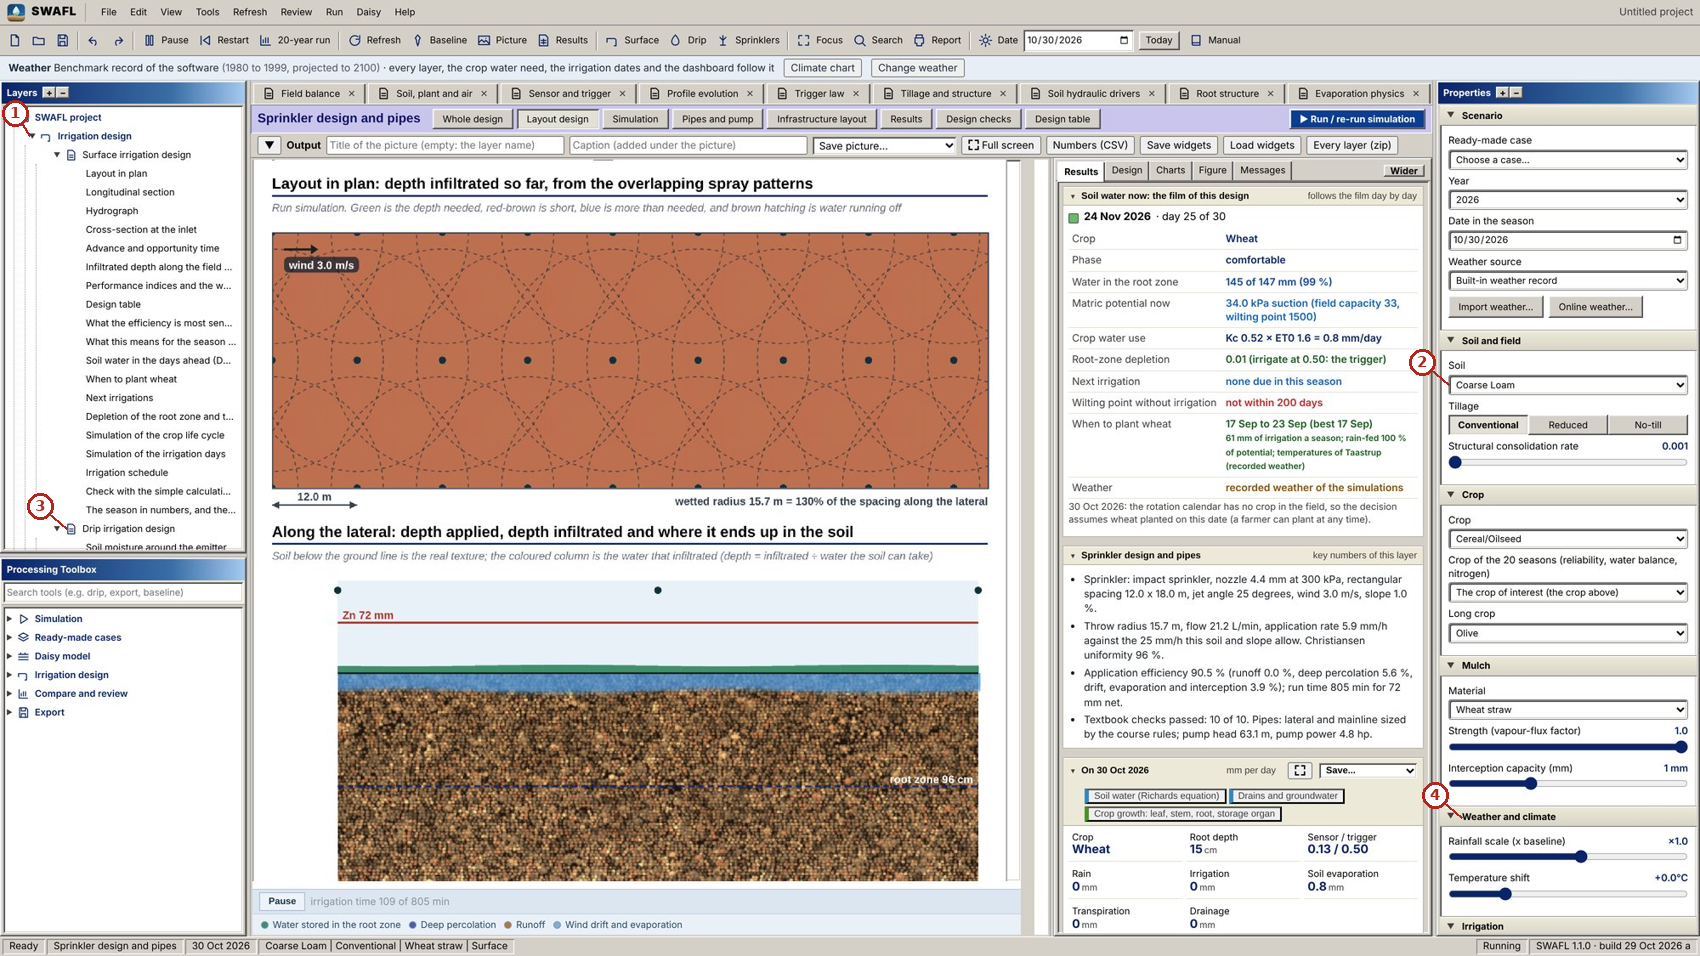
\includegraphics[width=\textwidth,height=0.42\textheight,keepaspectratio]{../figures/annot/p2_fig-shot-spr-sec-intake_0.png}\end{center}

\textbf{What the numbered labels point to (picture 1 of 2: Sprinkler: layout in plan, with the depth infiltrated from the overlapping spray patterns.).}
\begin{enumerate}[nosep,label=\protect\circled{\arabic*}]
\item ``Irrigation design'': the irrigation-design group of the Layers tree and its layers.
\item ``Coarse Loam v'': the soil of the project, which every layer uses.
\item ``Drip irrigation design'': the irrigation-design group of the Layers tree and its layers.
\item ``Weather and climate'': the weather of the project: built-in record, a file of the user or online weather of any place.
\end{enumerate}

\begin{center}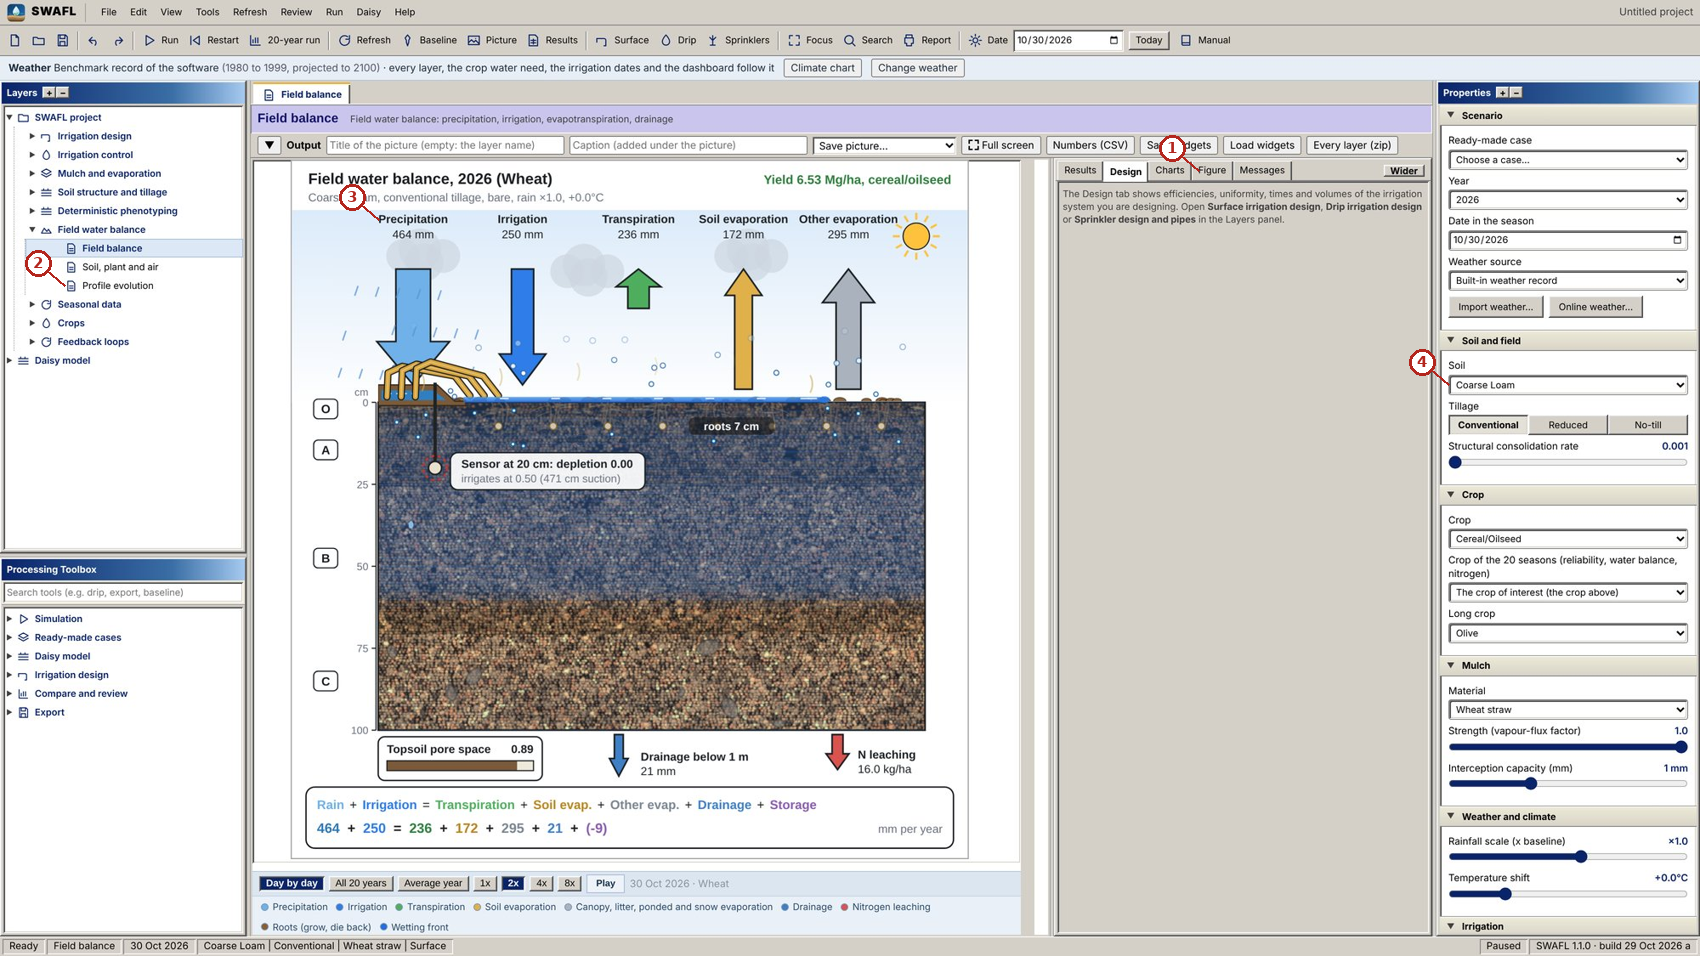
\includegraphics[width=\textwidth,height=0.42\textheight,keepaspectratio]{../figures/annot/p2_fig-shot-spr-sec-intake_1.png}\end{center}

\textbf{What the numbered labels point to (picture 2 of 2: Dashboard with the design tab open beside the field-balance layer.).}
\begin{enumerate}[nosep,label=\protect\circled{\arabic*}]
\item ``Figure'': a heading or control of this screen; the caption above says which layer it belongs to.
\item ``Profile evolution'': a heading or control of this screen; the caption above says which layer it belongs to.
\item ``Precipitation'': rain, from the weather of the project.
\item ``Coarse Loam v'': the soil of the project, which every layer uses.
\end{enumerate}

\textbf{What it shows.} SWAFL Desktop: sprinkler intake and the dashboard. Panels: (a) Sprinkler: layout in plan, with the depth infiltrated from the overlapping spray patterns. (b) Dashboard with the design tab open beside the field-balance layer.

\textbf{How to read the labels, symbols and colours.} A screen of the software as it appears to the user; the labelled areas are the inputs, the figure and the numbers of the layer named in the caption.

\textbf{What affects it, and why it happens.} Where the application rate exceeds the intake rate of the soil, water ponds and runs off. 

\textbf{How it is made.} Screen capture of SWAFL Desktop 1.1.0 (not regenerated).


\subsection{Derivation: Drip laterals}\label{der:s2:11}
The Hazen--Williams friction loss over a pipe segment of length $\Delta x$ carrying $Q_j$ is $h_{f,j}=10.67\Delta x\,Q_j^{1.852}/(C^{1.852}D^{4.871})$. Along a lateral with $N$ equal outlets the flow falls linearly towards the end; summing the losses of the segments, $h_f=\frac{10.67LQ_0^{1.852}}{C^{1.852}D^{4.871}}\frac1{N^{2.852}}\sum_{j=1}^{N}j^{1.852}$. The Euler--Maclaurin formula gives $\sum_{j=1}^Nj^{m}\simeq\frac{N^{m+1}}{m+1}+\frac{N^m}{2}+\dots$ with $m=1.852$, so the loss is the full-flow loss times $F_c=\frac1{m+1}+\frac1{2N}+\dots$; \citet{Christiansen1942} approximated the remaining terms by $\sqrt{m-1}/(6N^2)$, which gives the factor of the paper, $F_c=\frac1{2.852}+\frac1{2N}+\frac{\sqrt{0.852}}{6N^2}$. Each emitter discharges $q_j=q(h_j/H_0)^{x_e}$, which couples the flows to the heads and is solved by iteration.


\subsection{Derivation: Emission uniformity}\label{der:s2:12}
For emitters with manufacturing variation $c_v$ and $n_e$ emitters per plant, the lower quarter of plant flows lies about $1.27c_v/\sqrt{n_e}$ below the mean (normal distribution), and the hydraulic variation adds the ratio $q_{\min}/\bar q$; their product is the design emission uniformity of \citet{KellerKarmeli1974}.


\subsection{Derivation: Sprinkler discharge}\label{der:s2:13}
Bernoulli's equation across a nozzle gives the jet speed $v=\sqrt{2gh_n}$, and the discharge is $q=C_dA_n\sqrt{2gh_n}$ with $C_d\approx0.95$; the factor $6\times10^4$ converts m$^3$\,s$^{-1}$ to L\,min$^{-1}$. The Christiansen coefficient of uniformity is $CU=1-\sum|z_i-\bar z|/(n\bar z)$.




\section{Every term of the author's equations}
\subsection*{Soil-specific trigger, $h^\ast=\alpha^{-1}([S_e(100)-f^\ast\{S_e(100)-S_e(15\,849)\}]^{-1/m}-1)^{1/n}$}
{\small\begin{longtable}{>{\raggedright\arraybackslash}p{\dimexpr 0.1447\linewidth-2\tabcolsep\relax}>{\raggedright\arraybackslash}p{\dimexpr 0.2763\linewidth-2\tabcolsep\relax}>{\raggedright\arraybackslash}p{\dimexpr 0.1316\linewidth-2\tabcolsep\relax}>{\raggedright\arraybackslash}p{\dimexpr 0.2105\linewidth-2\tabcolsep\relax}>{\raggedright\arraybackslash}p{\dimexpr 0.2368\linewidth-2\tabcolsep\relax}}\toprule Term & What it means & Unit & Where the value comes from & When it rises\\\midrule\endhead
$f^\ast$ & chosen depletion of the plant-available water & -- & agronomy (0.45) & $h^\ast$ rises (drier trigger)\\
$S_e(100)$ & effective saturation at field capacity & -- & retention curve & $h^\ast$ shifts\\
$S_e(15\,849)$ & effective saturation at the wilting point & -- & retention curve & $h^\ast$ shifts\\
$\alpha$, $n$, $m$ & van~Genuchten parameters & cm$^{-1}$, --, -- & soil table & see the reach equations\\
$h^\ast$ & suction at which the soil has used $f^\ast$ of its water & cm & computed & --\\
\bottomrule\end{longtable}}
\subsection*{Interception store, $I_c=\mu_0\ln(1/r)$}
{\small\begin{longtable}{>{\raggedright\arraybackslash}p{\dimexpr 0.1447\linewidth-2\tabcolsep\relax}>{\raggedright\arraybackslash}p{\dimexpr 0.2763\linewidth-2\tabcolsep\relax}>{\raggedright\arraybackslash}p{\dimexpr 0.1316\linewidth-2\tabcolsep\relax}>{\raggedright\arraybackslash}p{\dimexpr 0.2105\linewidth-2\tabcolsep\relax}>{\raggedright\arraybackslash}p{\dimexpr 0.2368\linewidth-2\tabcolsep\relax}}\toprule Term & What it means & Unit & Where the value comes from & When it rises\\\midrule\endhead
$\mu_0$ & mean daily rain on rain days & mm & weather & $I_c$ rises in proportion\\
$r$ & throughfall fraction of the annual model & -- & Engine 1 & $I_c$ falls\\
\bottomrule\end{longtable}}
\subsection*{Two-stage evaporation, $Q(t)=Q_1+2e_0\tau_E(\sqrt{1+(t-t_1)/\tau_E}-1)$}
{\small\begin{longtable}{>{\raggedright\arraybackslash}p{\dimexpr 0.1447\linewidth-2\tabcolsep\relax}>{\raggedright\arraybackslash}p{\dimexpr 0.2763\linewidth-2\tabcolsep\relax}>{\raggedright\arraybackslash}p{\dimexpr 0.1316\linewidth-2\tabcolsep\relax}>{\raggedright\arraybackslash}p{\dimexpr 0.2105\linewidth-2\tabcolsep\relax}>{\raggedright\arraybackslash}p{\dimexpr 0.2368\linewidth-2\tabcolsep\relax}}\toprule Term & What it means & Unit & Where the value comes from & When it rises\\\midrule\endhead
$e_0$ & evaporative demand (stage-1 rate) & mm\,d$^{-1}$ & weather & $Q$ rises\\
$Q_1$ & cumulative evaporation at the end of stage 1 & mm & soil texture & stage 1 lasts longer\\
$t_1$ & end of stage 1 & d & $(Q_1-q_0)/e_0$ & --\\
$\tau_E$ & transition time of stage 2 & d & soil & stage 2 decays more slowly\\
\bottomrule\end{longtable}}


\section{How every constant is obtained, what it depends on, and how sensitive the results are}
\subsection{How every constant of the article is obtained}
{\small\begin{longtable}{>{\raggedright\arraybackslash}p{\dimexpr 0.1974\linewidth-2\tabcolsep\relax}>{\raggedright\arraybackslash}p{\dimexpr 0.1382\linewidth-2\tabcolsep\relax}>{\raggedright\arraybackslash}p{\dimexpr 0.3553\linewidth-2\tabcolsep\relax}>{\raggedright\arraybackslash}p{\dimexpr 0.3092\linewidth-2\tabcolsep\relax}}
\toprule Constant & Value & How it was obtained & What it depends on; sensitivity\\\midrule\endhead
$f^\ast$, critical depletion & 0.45 & from the simulations: the depletion beyond which the simulated yield falls by more than 5\,\% & the crop and the 5\,\% tolerance; a larger $f^\ast$ gives drier triggers\\
Field capacity, wilting point & 100\,cm, 15\,849\,cm & FAO convention \citep{Allen1998} (pF 2 and pF 4.2) & a different field capacity shifts every depletion\\
Rain-day fraction in $\mu_0=P/(0.28\cdot365)$ & 0.28 & engineered: about one day in four is a rain day in the benchmark weather & the climate; $I_c$ scales with $\mu_0$\\
Throughfall $r$ & $\max(40,P-P_{\mathrm{other}})/P$ & chosen so that the daily model intercepts what the annual model intercepts & Engine 1\\
Stage-1 depth $L_1$ & 40\,mm & engineered: the layer that dries in stage 1 & a deeper layer lengthens stage 1\\
Surface-dry suction $h_s$ & $4/\alpha$ & engineered, scaled by $\alpha$ so it samples the steep part of every curve & the soil\\
Stage-2 time $\tau_E$ & $0.006+0.03(\mathrm{clay}+\mathrm{silt})/100$\,d & engineered: finer soils supply the surface longer & the texture\\
Surface tension, contact angle & 0.0728\newline N\,m$^{-1}$; 0 & physical constants of water at 20\,$^\circ$C \citep{Hillel1998} & temperature; repellent soils have a larger angle\\
Kelvin factor & 135.3\,MPa & $\mathcal RT_K/V_w$ at 20\,$^\circ$C & temperature\\
Nozzle coefficient & 0.95 & typical discharge coefficient of a sprinkler nozzle & the nozzle\\
Hazen--Williams exponent & 1.852 & from the Hazen--Williams formula & the pipe; $C$ depends on the material\\
Keller--Karmeli factor & 1.27 & from the normal distribution of emitter flows \citep{KellerKarmeli1974} & the manufacturing variation\\\bottomrule
\end{longtable}}


\section{How each table of the article is produced}
\paragraph{Table 1 of the article.} \emph{Symbols, abbreviations and units of the soil--water--atmosphere engines and of the irrigation design modules, grouped by subject.}

\textbf{How it is made.} Table typed from the result file (4 of its numbers found there). Script: \nolinkurl{Manuscripts/reproducibility/audit_numbers.py}. Input: \nolinkurl{Data/daisy_ensemble.csv.gz}.

\paragraph{Table 2 of the article.} \emph{State variables and fluxes of the modelled soil--water--atmosphere system, by compartment; the soil matrix and soil structure rows form the soil compartment, and the lower boundary (drainage) and the management decision are listed separately. Source: E1 = Engine~1 (annual), E2 = Engine~2 (daily), D = Daisy output stored in the software, R = relation evaluated by the layer. Provenance: L literature, D data-driven, E engineered.}

\textbf{How it is made.} Table typed from the result file (10 of its numbers found there). Script: \nolinkurl{Manuscripts/reproducibility/audit_numbers.py}. Input: \nolinkurl{Data/daisy_ensemble.csv.gz}.

\paragraph{Table 3 of the article.} \emph{The twelve controls of the framework, their values and defaults, and the variables that respond. Run set: the Daisy experiment from which the response is read.}

\textbf{How it is made.} Table typed from the result file (5 of its numbers found there). Script: \nolinkurl{Manuscripts/reproducibility/p3_js/run_drip.js}. Input: \nolinkurl{Data/daisy_ensemble.csv.gz}.

\paragraph{Table 4 of the article.} \emph{The seven feedback loops: control step, printed effect and arrow-width input $\mu$.}

\textbf{How it is made.} Table typed in the manuscript from the result files of the script. Script: \nolinkurl{(see the reproducibility appendix of the paper)}. Input: \nolinkurl{Data/daisy_ensemble.csv.gz}.

\paragraph{Table 5 of the article.} \emph{Experiments used by Engine~1, the number of soils they cover and the equation family that consumes them.}

\textbf{How it is made.} Descriptive table (definitions, design, parameters or tests); no computation.

\paragraph{Table 6 of the article.} \emph{Output variables of each Daisy run (20-year means, 1980--1999) that form the evidence layer. The complete run table is in the \datalink{} folder of the repository and on Zenodo.}

\textbf{How it is made.} Descriptive table (definitions, design, parameters or tests); no computation.

\paragraph{Table 7 of the article.} \emph{Effective van~Genuchten parameters used by Engine~1 and the available-water capacity (AWC, mm of water per cm of soil, an engineered texture-class constant), with the critical suction $h^\ast$ at the soil-independent depletion $f^\ast=0.45$.}

\textbf{How it is made.} Table typed from the result file (11 of its numbers found there). Script: \nolinkurl{Manuscripts/reproducibility/audit_numbers.py}. Input: \nolinkurl{Data/daisy_ensemble.csv.gz}.

\paragraph{Table 8 of the article.} \emph{Soil and surface variables of the ten soils. Texture as sand/silt/clay (\%); $\theta_s$, $\theta_r$ from Eq.~(2) of the article; $S_e(100)$ effective saturation at field capacity; $f(300)$ depletion reached at a suction of 300\,cm (Eq.~(29) of the article); $Q_1$ stage-1 storage, $\tau_E$ stage-2 time scale, $t_1$ stage-1 duration and $Q(12)$ cumulative evaporation after 12 days at $e_0=4.2$\,mm\,d$^{-1}$ (Eq.~(11) of the article).}

\textbf{How it is made.} Table typed from the result file (39 of its numbers found there). Script: \nolinkurl{Manuscripts/reproducibility/p3_js/run_drip.js}. Input: \nolinkurl{Data/daisy_ensemble.csv.gz}.

\paragraph{Table 9 of the article.} \emph{Annual balance of the ten soils from Engine~1 (mm\,yr$^{-1}$, 20-year means; Eq.~(1) of the article): precipitation $P$, irrigation $I$, transpiration $T$, soil evaporation $E$, other evaporation $E_{\mathrm{oth}}$, drainage $D$ and storage change $\Delta S$; yield $Y$ (Mg\,ha$^{-1}$), nitrate leaching $N_L$ (kg\,ha$^{-1}$\,yr$^{-1}$) and the regime index $\mathcal I$ (Eq.~(14) of the article).}

\textbf{How it is made.} Table typed from the result file (15 of its numbers found there). Script: \nolinkurl{Manuscripts/reproducibility/audit_numbers.py}. Input: \nolinkurl{Data/daisy_ensemble.csv.gz}.

\paragraph{Table 10 of the article.} \emph{Crop, water-potential and mulch variables of the ten soils. Engine~2 (20 years): maximum rooting depth $R_{\max}$ (Eq.~(17) of the article), mean of the yearly deepest roots $\bar R_d$, depths holding 50 and 90\,\% of uptake (Eq.~(20) of the article), irrigation events per year, dose $d$ (mm), median wetting depth of an irrigation (cm) and calibration factor $k_t$. Water-potential path (Eq.~(21) and Eq.~(22) of the article), means over crop days of day-of-year 120--210: $\psi_{\mathrm{RZ}}$, $\psi_{\mathrm{leaf}}$ (MPa) and share of days with $\psi_{\mathrm{leaf}}<-1.6$\,MPa. Straw mulch ($\varphi=0.4$, $c=4$\,mm) against bare soil: evaporation saved $\Delta E$ (mm\,yr$^{-1}$) and its fate shares (Eq.~(23) of the article).}

\textbf{How it is made.} Table typed from the result file (36 of its numbers found there). Script: \nolinkurl{Manuscripts/reproducibility/p3_js/swa_vars.js}. Input: \nolinkurl{Data/daisy_ensemble.csv.gz}.

\paragraph{Table 11 of the article.} \emph{Result views, governing relations and verification. Equation numbers in brackets refer to the Manual; provenance labels are L (literature), D (data-driven), E (engineered).}

\textbf{How it is made.} Table typed from the result file (11 of its numbers found there). Script: \nolinkurl{Manuscripts/reproducibility/audit_numbers.py}. Input: \nolinkurl{Data/daisy_ensemble.csv.gz}.

\paragraph{Table 12 of the article.} \emph{Surface-irrigation Example 6.1 \citep{Walker1987}: published and computed quantities. $T_{req}$: required infiltration time (min); $t_L$: advance time to the end of the furrow (min) at flow $Q$ (m$^3$\,min$^{-1}$); $E_a$: application efficiency (\%). Error $=100(\text{SWAFL}-\text{book})/\text{book}$.}

\textbf{How it is made.} Table typed from the result file (22 of its numbers found there). Script: \nolinkurl{Manuscripts/reproducibility/audit_numbers.py}. Input: \nolinkurl{Data/daisy_ensemble.csv.gz}.

\paragraph{Table 13 of the article.} \emph{Border Example 6.4 (\citet{Walker1987}) and the sprinkler example: published and computed values.}

\textbf{How it is made.} Table typed from the result file (11 of its numbers found there). Script: \nolinkurl{Manuscripts/reproducibility/run_all.sh}. Input: \nolinkurl{Data/daisy_ensemble.csv.gz}.

\paragraph{Table 14 of the article.} \emph{Engine 1 against 1\,000 held-out E12 runs (coarse loam), off-axis cells. Raw: as shipped; re-anchored: baseline aligned. nRMSE: RMSE as \% of the observed mean; $\rho$: Spearman rank correlation.}

\textbf{How it is made.} Table typed from the result file (15 of its numbers found there). Script: \nolinkurl{Manuscripts/reproducibility/run_all.sh}. Input: \nolinkurl{Data/daisy_ensemble.csv.gz}.

\paragraph{Table 15 of the article.} \emph{Drip lateral solver of version~1 (four passes) and the converged solver against an independent solver, by loss ratio $h_f/H_0$ (400 random configurations). Maximum relative error in $h_f$ and maximum absolute error in $E_u$.}

\textbf{How it is made.} Table typed from the result file (4 of its numbers found there). Script: \nolinkurl{Manuscripts/reproducibility/p3_js/run_drip.js}. Input: \nolinkurl{Data/daisy_ensemble.csv.gz}.

\paragraph{Table 16 of the article.} \emph{What this article adds, item by item: what was established before, what is new here, and the evidence in this article.}

\textbf{How it is made.} Table typed from the result file (4 of its numbers found there). Script: \nolinkurl{Manuscripts/reproducibility/audit_numbers.py}. Input: \nolinkurl{Data/daisy_ensemble.csv.gz}.


\section{From the data to every result: experiments, runs and computations}\label{sec:prov}
\paragraph{Where every number starts.} All simulated numbers come from one set of 10\,190 Daisy runs, organised in seventeen experiments (E0 to E16), each of which varies a few factors on the same ten soils (S01 to S10) under the same weather series (Taastrup, Denmark). Every run writes 20-year mean annual fluxes (rain, irrigation, evapotranspiration and its parts, drainage at 1\,m, yield, nitrogen); one row per run is stored in \nolinkurl{Data/Comprehensive_Summary/00_summary_all_simulations.csv.gz} (sheet \texttt{All\_runs\_summary} of the workbook) and, for the ensemble analyses, in \nolinkurl{Data/daisy_ensemble.csv.gz} (sheet \texttt{Ensemble\_runs}). A run is used only when its status is \texttt{ok} (10\,041 runs); the 149 runs whose solver failed are kept in the files but never enter a result. The workbook repeats the per-run algebra as live Excel formulas (the green columns at the end of \texttt{All\_runs\_summary}: other evaporation, balance residual, differences from the rainfed run of the same soil, water productivity), and the sheet \texttt{Column\_Equations} lists the equation behind every calculated column. The rainfed run of each soil (experiment E0) is the reference against which every irrigated or treated run is compared (sheet \texttt{Baselines\_E0}).

{\footnotesize\begin{longtable}{>{\raggedright\arraybackslash}p{\dimexpr 0.1667\linewidth-2\tabcolsep\relax}>{\raggedright\arraybackslash}p{\dimexpr 0.2051\linewidth-2\tabcolsep\relax}>{\raggedright\arraybackslash}p{\dimexpr 0.3974\linewidth-2\tabcolsep\relax}>{\raggedright\arraybackslash}p{\dimexpr 0.2308\linewidth-2\tabcolsep\relax}}
\toprule Result & Experiment and runs & How it is computed from the runs & Script, file, workbook\\\midrule\endhead
Critical depletion $f^\ast=0.45$ & E2\_\allowbreak{}TriggerPressure (197 valid runs; soils with a maximum irrigation above 50\,mm) & the trigger of every run is turned into a root-zone depletion $f$ (two horizons, 0--25 and 25--100\,cm, field capacity 100\,cm, wilting point 15\,849\,cm); relative yield $Y/Y_{\max}$ of the soil; median of $Y/Y_{\max}$ in 15 bins of $f$; $f^\ast$ is the first bin after the peak whose median falls below 0.95 & \texttt{Results/08\_\allowbreak{}Scripts/novel.py}; \texttt{D\_\allowbreak{}N1\_\allowbreak{}soil\_\allowbreak{}specific\_\allowbreak{}triggers}\\
Soil-specific triggers $h^\ast$ (143--729\,cm) & $\alpha$, $n$ of the soils and $f^\ast$ & solve $f(h)=f^\ast$ for $h$ (the closed form derived in this supplement) & live formulas in \texttt{D\_\allowbreak{}N1\_\allowbreak{}soil\_\allowbreak{}specific\_\allowbreak{}triggers}, \texttt{EQ\_\allowbreak{}P2}; chart \texttt{CH\_\allowbreak{}P2}\\
Share of the available water used at 300\,cm (24--84\,\%) & same & $f(300)$ for each soil & column \texttt{f\_\allowbreak{}at\_\allowbreak{}300}\\
Soil--water--atmosphere variables of the ten soils & the soil parameters of the model & evaluated by the program's own functions (capillary radius, conductivity, evaporation stages, air potential) & \texttt{p3\_\allowbreak{}js/swa\_\allowbreak{}vars.js} $\to$ \texttt{p3\_\allowbreak{}swa\_\allowbreak{}vars.json}; sheet \texttt{R\_\allowbreak{}p3\_\allowbreak{}swa\_\allowbreak{}vars}\\
Interception store matched to the annual model & daily rain as an exponential distribution with mean $\mu_0$ & throughfall above a store $I_c$ integrated over the distribution and set equal to the annual throughfall fraction & live formula in \texttt{EQ\_\allowbreak{}P2}\\
Sensitivity of the outputs to the controls & E1\_\allowbreak{}Doses, E3, E4, E7 and E12 & per-soil relative change of yield, drainage and irrigation per lever (\texttt{lev\_\allowbreak{}pct}) and its rank correlation with the available water & \texttt{D\_\allowbreak{}controllability\_\allowbreak{}by\_\allowbreak{}soil\_\allowbreak{}lever}, \texttt{D\_\allowbreak{}controllability\_\allowbreak{}rho\_\allowbreak{}vs\_\allowbreak{}TAW}\\
Verification of every computing layer & textbook examples and the shipped engines & each layer recomputes a published example (surface irrigation, drip lateral, sprinkler, FAO-56) and the difference is reported & \texttt{p3\_\allowbreak{}js/*.js} $\to$ \texttt{p3\_\allowbreak{}surface*.json}, \texttt{drip\_\allowbreak{}out.json}, \texttt{spr\_\allowbreak{}out.json}, \texttt{fao\_\allowbreak{}out.json}; sheets \texttt{R\_\allowbreak{}*}\\\bottomrule
\end{longtable}}


\section{The data}
\Cref{tab:data} lists the 17 experiments of the data folder and \cref{fig:data} shows their outputs. The tables that follow are the result files of the analyses of the paper, printed in full or up to 220 rows; each is also in the workbook \nolinkurl{Data/Manuscript_Data/SWAFL_Manuscripts_Data.xlsx}, and every run is in \cslink.
\begin{table}[H]\centering\scriptsize
\caption{The data of this study: the 17 Daisy experiments of \texttt{Data/Comprehensive\_Summary} (10190 runs, 10041 valid; 20 years, 1980--1999, of Taastrup weather). Means of the valid runs; $Y$ yield (Mg\,ha$^{-1}$), $I$ irrigation, $D$ drainage at 1\,m and $\ET$ (mm\,yr$^{-1}$), $N_L$ nitrate leached (kg\,N\,ha$^{-1}$\,yr$^{-1}$), $t$ run time of Daisy (s). Every row is one file of the folder, linked.}
\label{tab:data}
\setlength{\tabcolsep}{3pt}
\begin{tabular}{@{}llrrp{3.5cm}rrrrrr@{}}
\toprule
Exp. & File & Runs & Valid & Factors varied & $Y$ & $I$ & $D$ & $\ET$ & $N_L$ & $t$\\\midrule
E0 & \href{\repourl/blob/main/Data/Comprehensive_Summary/E00_Baselines.csv.gz}{\texttt{Baselines}} & 10 & 10 & soil & 2.19 & 0 & 55 & 418 & 158 & 231\\
E1 & \href{\repourl/blob/main/Data/Comprehensive_Summary/E01_Doses.csv.gz}{\texttt{Doses}} & 200 & 189 & soil, rate, dose & 5.13 & 198 & 98 & 564 & 79 & 195\\
E2 & \href{\repourl/blob/main/Data/Comprehensive_Summary/E02_TriggerPressure.csv.gz}{\texttt{TriggerPressure}} & 200 & 197 & soil, trigger & 4.70 & 169 & 80 & 559 & 90 & 139\\
E3 & \href{\repourl/blob/main/Data/Comprehensive_Summary/E03_SensorDepth.csv.gz}{\texttt{SensorDepth}} & 200 & 200 & soil, sensor depth & 4.94 & 199 & 86 & 583 & 86 & 146\\
E4 & \href{\repourl/blob/main/Data/Comprehensive_Summary/E04_Methods.csv.gz}{\texttt{Methods}} & 100 & 96 & soil, method & 5.01 & 164 & 88 & 542 & 83 & 147\\
E5 & \href{\repourl/blob/main/Data/Comprehensive_Summary/E05_SHP_Dynamics.csv.gz}{\texttt{SHP Dynamics}} & 300 & 300 & soil, method, tillage & 4.13 & 152 & 43 & 579 & 84 & 189\\
E6 & \href{\repourl/blob/main/Data/Comprehensive_Summary/E06_Mediterranean_Pollution.csv.gz}{\texttt{Mediterranean Pollution}} & 210 & 193 & soil, method, trigger, N rate & 3.64 & 84 & 239 & 620 & 62 & 118\\
E7 & \href{\repourl/blob/main/Data/Comprehensive_Summary/E07_Mulching.csv.gz}{\texttt{Mulching}} & 200 & 200 & soil, mulch & 5.29 & 183 & 96 & 555 & 74 & 161\\
E8 & \href{\repourl/blob/main/Data/Comprehensive_Summary/E08_Rain_Intensity_Moisture.csv.gz}{\texttt{Rain Intensity Moisture}} & 1000 & 1000 & initial suction, rain scale & 0.68 & 0 & -1 & 282 & -0 & 6\\
E9 & \href{\repourl/blob/main/Data/Comprehensive_Summary/E09_Soil_Moisture_Rain.csv.gz}{\texttt{Soil Moisture Rain}} & 1000 & 987 & soil, initial suction, rain scale & 0.75 & 0 & 19 & 247 & 33 & 7\\
E10 & \href{\repourl/blob/main/Data/Comprehensive_Summary/E10_Amount_Timing_Soil.csv.gz}{\texttt{Amount Timing Soil}} & 1000 & 954 & soil, rate, dose, window & 4.42 & 139 & 76 & 532 & 97 & 146\\
E11 & \href{\repourl/blob/main/Data/Comprehensive_Summary/E11_Temp_Evap_Rain.csv.gz}{\texttt{Temp Evap Rain}} & 1000 & 1000 & rain scale, warming, demand & 3.81 & 324 & 18 & 754 & 66 & 151\\
E12 & \href{\repourl/blob/main/Data/Comprehensive_Summary/E12_Sensor_Trigger_Rain.csv.gz}{\texttt{Sensor Trigger Rain}} & 1000 & 1000 & trigger, sensor depth, rain scale & 5.88 & 260 & 35 & 670 & 32 & 155\\
E13 & \href{\repourl/blob/main/Data/Comprehensive_Summary/E13_N_Water_Soil.csv.gz}{\texttt{N Water Soil}} & 1000 & 975 & soil, method, rate, dose, trigger, N rate & 4.00 & 162 & 83 & 547 & 79 & 207\\
E14 & \href{\repourl/blob/main/Data/Comprehensive_Summary/E14_Mulch_Rain.csv.gz}{\texttt{Mulch Rain}} & 1000 & 1000 & rain scale, mulch & 6.15 & 235 & 43 & 634 & 25 & 173\\
E15 & \href{\repourl/blob/main/Data/Comprehensive_Summary/E15_Method_Depth_Amount.csv.gz}{\texttt{Method Depth Amount}} & 1000 & 1000 & method, rate, dose, root depth & 6.02 & 217 & 61 & 619 & 37 & 157\\
E16 & \href{\repourl/blob/main/Data/Comprehensive_Summary/E16_Edge_Cases.csv.gz}{\texttt{Edge Cases}} & 770 & 740 & soil, method, rate, dose, trigger, sensor depth, rain scale, warming, N rate, demand & 2.17 & 344 & 185 & 600 & 93 & 224\\
\bottomrule
\end{tabular}
\end{table}

\begin{figure}[H]\centering
\includegraphics[width=\textwidth]{\figdir/data/fig_data_overview.pdf}
\caption{Yield, irrigation, drainage and nitrate leaching of the valid runs, by experiment.}\label{fig:data}
\end{figure}
\subsection*{p3\_swa\_vars.json}
\noindent\small Source: \nolinkurl{Manuscripts/results/p3_swa_vars.json}; 650 values, first 220 shown. Workbook sheet \texttt{R\_p3\_swa\_vars}.\par
{\scriptsize\begin{longtable}{p{\dimexpr 0.4557\linewidth-2\tabcolsep\relax}p{\dimexpr 0.5443\linewidth-2\tabcolsep\relax}}\toprule\textbf{quantity} & \textbf{value}\\\midrule\endhead
{}[0].soil & S01\_CoarseLoam\\
{}[0].label & Coarse Loam\\
{}[0].hyd.alpha & 0.09613\\
{}[0].hyd.n & 1.353\\
{}[0].hyd.sand & 45\\
{}[0].hyd.silt & 35\\
{}[0].hyd.clay & 20\\
{}[0].hyd.thetaS & 0.4235\\
{}[0].hyd.thetaR & 0.022\\
{}[0].hyd.AWC & 1.5\\
{}[0].hyd.f300 & 0.3795\\
{}[0].hyd.hStar & 387.3\\
{}[0].hyd.Se100 & 0.4443\\
{}[0].e1.evap & 174.6\\
{}[0].e1.transp & 239\\
{}[0].e1.et & 720.3\\
{}[0].e1.irr & 282.2\\
{}[0].e1.yield & 6.627\\
{}[0].e1.drain & 27.62\\
{}[0].e1.nl & 14.56\\
{}[0].e1.rain & 464\\
{}[0].e1.other & 306.7\\
{}[0].e1.store & -1.67\\
{}[0].e1.ie & 2.348\\
{}[0].e2.Rmax & 93.58\\
{}[0].e2.meanRootMax & 89.94\\
{}[0].e2.z50 & 19.25\\
{}[0].e2.z90 & 47\\
{}[0].e2.kt & 1.641\\
{}[0].e2.dose & 28.22\\
{}[0].e2.fTrig & 0.3795\\
{}[0].e2.irrMean & 283.7\\
{}[0].e2.eventsPerYear & 10.05\\
{}[0].e2.uptakeProfile & 30.27, 24.66, 23.52, 22.37, 22.36, 21.16, 19.86, 18.68, 20.95, 14.61, 13.69, 12.82 ... (40 values)\\
{}[0].e2.sProfile & 0.4658, 0.5419, 0.6077, 0.6541, 0.7093, 0.7365, 0.7559, 0.7728, 0.7867, 0.7988, 0.81, 0.821 ... (40 values)\\
{}[0].e2.wetFrontIrr & 45\\
{}[0].e2.drainUnscaled & 7.334\\
{}[0].e2.interceptionUnscaled & 312.7\\
{}[0].e2.evapUnscaled & 117\\
{}[0].e2.transpUnscaled & 335.7\\
{}[0].spac.psiRZ & -0.0494\\
{}[0].spac.psiRoot & -1.814\\
{}[0].spac.psiLeaf & -2.243\\
{}[0].spac.Kr & 8.391e-06\\
{}[0].spac.closedShare & 0.7405\\
{}[0].spac.psiAir & -56.3\\
{}[0].spac.days & 1715\\
{}[0].evap.e0 & 4.2\\
{}[0].evap.Q1 & 5.991\\
{}[0].evap.tau & 0.0225\\
{}[0].evap.t1 & 1.426\\
{}[0].evap.lost12 & 9.903\\
{}[0].evap.dtheta & 0.3514\\
{}[0].evap.hi & 2.601\\
{}[0].evap.hs & 41.61\\
{}[0].mulch.dE & 127.4\\
{}[0].mulch.dI & 34.86\\
{}[0].mulch.dD & 7.26\\
{}[0].mulch.dT & 17.84\\
{}[0].mulch.fI & 0.2736\\
{}[0].mulch.fD & 0.05697\\
{}[0].mulch.fT & 0.14\\
{}[0].mulch.fRest & 0.5294\\
{}[0].regime & 0.7268\\
{}[0].kappaN & 0.3783\\
{}[1].soil & S02\_CoarseSand\\
{}[1].label & Coarse Sand\\
{}[1].hyd.alpha & 0.05358\\
{}[1].hyd.n & 1.6\\
{}[1].hyd.sand & 88\\
{}[1].hyd.silt & 8\\
{}[1].hyd.clay & 4\\
{}[1].hyd.thetaS & 0.3736\\
{}[1].hyd.thetaR & 0.0124\\
{}[1].hyd.AWC & 0.5\\
{}[1].hyd.f300 & 0.4964\\
{}[1].hyd.hStar & 261.9\\
{}[1].hyd.Se100 & 0.3563\\
{}[1].e1.evap & 117.8\\
{}[1].e1.transp & 236.7\\
{}[1].e1.et & 716.3\\
{}[1].e1.irr & 413.8\\
{}[1].e1.yield & 6.449\\
{}[1].e1.drain & 163.6\\
{}[1].e1.nl & 62.55\\
{}[1].e1.rain & 464\\
{}[1].e1.other & 361.8\\
{}[1].e1.store & -2.18\\
{}[1].e1.ie & 1.559\\
{}[1].e2.Rmax & 100\\
{}[1].e2.meanRootMax & 96.15\\
{}[1].e2.z50 & 24.5\\
{}[1].e2.z90 & 64.75\\
{}[1].e2.kt & 1.12\\
{}[1].e2.dose & 35\\
{}[1].e2.fTrig & 0.4964\\
{}[1].e2.irrMean & 423.5\\
{}[1].e2.eventsPerYear & 12.1\\
{}[1].e2.uptakeProfile & 8.878, 10.93, 12.22, 12.53, 13.49, 12.93, 12.01, 11.32, 11.73, 9.564, 8.149, 7.661 ... (40 values)\\
{}[1].e2.sProfile & 0.2935, 0.4015, 0.4911, 0.552, 0.6278, 0.6603, 0.6845, 0.7038, 0.7202, 0.7356, 0.7505, 0.7642 ... (40 values)\\
{}[1].e2.wetFrontIrr & 100\\
{}[1].e2.drainUnscaled & 259\\
{}[1].e2.interceptionUnscaled & 369.4\\
{}[1].e2.evapUnscaled & 61.06\\
{}[1].e2.transpUnscaled & 219.3\\
{}[1].spac.psiRZ & -0.03899\\
{}[1].spac.psiRoot & -1.848\\
{}[1].spac.psiLeaf & -2.275\\
{}[1].spac.Kr & 5.581e-05\\
{}[1].spac.closedShare & 0.7504\\
{}[1].spac.psiAir & -56.3\\
{}[1].spac.days & 1715\\
{}[1].evap.e0 & 4.2\\
{}[1].evap.Q1 & 7.849\\
{}[1].evap.tau & 0.0096\\
{}[1].evap.t1 & 1.869\\
{}[1].evap.lost12 & 10.39\\
{}[1].evap.dtheta & 0.3392\\
{}[1].evap.hi & 4.666\\
{}[1].evap.hs & 74.66\\
{}[1].mulch.dE & 102.5\\
{}[1].mulch.dI & 51.11\\
{}[1].mulch.dD & 7.26\\
{}[1].mulch.dT & 14.76\\
{}[1].mulch.fI & 0.4988\\
{}[1].mulch.fD & 0.07086\\
{}[1].mulch.fT & 0.1441\\
{}[1].mulch.fRest & 0.2862\\
{}[1].regime & -0.1628\\
{}[1].kappaN & 0.3783\\
{}[2].soil & S03\_Sand\\
{}[2].label & Sand\\
{}[2].hyd.alpha & 0.145\\
{}[2].hyd.n & 2.68\\
{}[2].hyd.sand & 92\\
{}[2].hyd.silt & 5\\
{}[2].hyd.clay & 3\\
{}[2].hyd.thetaS & 0.3693\\
{}[2].hyd.thetaR & 0.0118\\
{}[2].hyd.AWC & 0.6\\
{}[2].hyd.f300 & 0.8422\\
{}[2].hyd.hStar & 142.8\\
{}[2].hyd.Se100 & 0.01119\\
{}[2].e1.evap & 58.2\\
{}[2].e1.transp & 202.3\\
{}[2].e1.et & 669\\
{}[2].e1.irr & 278.2\\
{}[2].e1.yield & 4.984\\
{}[2].e1.drain & 76.52\\
{}[2].e1.nl & 85.16\\
{}[2].e1.rain & 464\\
{}[2].e1.other & 408.5\\
{}[2].e1.store & -3.32\\
{}[2].e1.ie & 1.792\\
{}[2].e2.Rmax & 100\\
{}[2].e2.meanRootMax & 95.84\\
{}[2].e2.z50 & 27\\
{}[2].e2.z90 & 52.38\\
{}[2].e2.kt & 2.045\\
{}[2].e2.dose & 27.82\\
{}[2].e2.fTrig & 0.8422\\
{}[2].e2.irrMean & 285.1\\
{}[2].e2.eventsPerYear & 10.25\\
{}[2].e2.uptakeProfile & 14.55, 15.46, 16.02, 15.59, 16.18, 15.72, 15.22, 14.97, 15.88, 14.28, 13.66, 13.55 ... (40 values)\\
{}[2].e2.sProfile & 0.2917, 0.338, 0.3738, 0.396, 0.4246, 0.4392, 0.4515, 0.4625, 0.4765, 0.4922, 0.5086, 0.5228 ... (40 values)\\
{}[2].e2.wetFrontIrr & 55\\
{}[2].e2.drainUnscaled & 5.15\\
{}[2].e2.interceptionUnscaled & 424.5\\
{}[2].e2.evapUnscaled & 32.31\\
{}[2].e2.transpUnscaled & 314.8\\
{}[2].spac.psiRZ & -0.02021\\
{}[2].spac.psiRoot & -1.694\\
{}[2].spac.psiLeaf & -2.114\\
{}[2].spac.Kr & 2.075e-09\\
{}[2].spac.closedShare & 0.712\\
{}[2].spac.psiAir & -56.3\\
{}[2].spac.days & 1715\\
{}[2].evap.e0 & 4.2\\
{}[2].evap.Q1 & 12.71\\
{}[2].evap.tau & 0.0084\\
{}[2].evap.t1 & 3.027\\
{}[2].evap.lost12 & 14.95\\
{}[2].evap.dtheta & 0.3521\\
{}[2].evap.hi & 1.724\\
{}[2].evap.hs & 27.59\\
{}[2].mulch.dE & 49.62\\
{}[2].mulch.dI & 34.36\\
{}[2].mulch.dD & 7.26\\
{}[2].mulch.dT & 15.1\\
{}[2].mulch.fI & 0.6924\\
{}[2].mulch.fD & 0.1463\\
{}[2].mulch.fT & 0.3043\\
{}[2].mulch.fRest & 0\\
{}[2].regime & -0.136\\
{}[2].kappaN & 0.3783\\
{}[3].soil & S04\_LoamySand\\
{}[3].label & Loamy Sand\\
{}[3].hyd.alpha & 0.124\\
{}[3].hyd.n & 2.28\\
{}[3].hyd.sand & 82\\
{}[3].hyd.silt & 12\\
{}[3].hyd.clay & 6\\
{}[3].hyd.thetaS & 0.3804\\
{}[3].hyd.thetaR & 0.0136\\
{}[3].hyd.AWC & 0.9\\
{}[3].hyd.f300 & 0.7557\\
{}[3].hyd.hStar & 159.5\\
{}[3].hyd.Se100 & 0.03978\\
{}[3].e1.evap & 73.95\\
{}[3].e1.transp & 215\\
{}[3].e1.et & 691.2\\
{}[3].e1.irr & 293\\
{}[3].e1.yield & 5.456\\
{}[3].e1.drain & 70.14\\
{}[3].e1.nl & 61.13\\
{}[3].e1.rain & 464\\
{}[3].e1.other & 402.2\\
{}[3].e1.store & -4.31\\
{}[3].e1.ie & 1.862\\
{}[3].e2.Rmax & 100\\
\bottomrule\end{longtable}}

\subsection*{p3\_e1\_sens.json}
\noindent\small Source: \nolinkurl{Manuscripts/results/p3_e1_sens.json}; 223 values, first 220 shown. Workbook sheet \texttt{R\_p3\_e1\_sens}.\par
{\scriptsize\begin{longtable}{p{\dimexpr 0.4557\linewidth-2\tabcolsep\relax}p{\dimexpr 0.5443\linewidth-2\tabcolsep\relax}}\toprule\textbf{quantity} & \textbf{value}\\\midrule\endhead
{}base.irr & 282.2\\
{}base.et & 720.3\\
{}base.drain & 27.62\\
{}base.yield & 6.627\\
{}base.nl & 14.56\\
{}base.evap & 174.6\\
{}base.transp & 239\\
{}F[0].name & Rainfall scale\\
{}F[0].labLo & x0.7\\
{}F[0].labHi & x1.3\\
{}F[0].lo.irr & 430.2\\
{}F[0].lo.et & 725.9\\
{}F[0].lo.drain & 10.64\\
{}F[0].lo.yield & 3.655\\
{}F[0].lo.nl & 10.5\\
{}F[0].lo.evap & 124.6\\
{}F[0].lo.transp & 249\\
{}F[0].hi.irr & 188.7\\
{}F[0].hi.et & 719.2\\
{}F[0].hi.drain & 87.7\\
{}F[0].hi.yield & 6.633\\
{}F[0].hi.nl & 17.31\\
{}F[0].hi.evap & 199.9\\
{}F[0].hi.transp & 235.4\\
{}F[1].name & Warming\\
{}F[1].labLo & -1 C\\
{}F[1].labHi & +2 C\\
{}F[1].lo.irr & 224.1\\
{}F[1].lo.et & 643.4\\
{}F[1].lo.drain & 35.81\\
{}F[1].lo.yield & 6.633\\
{}F[1].lo.nl & 6.34\\
{}F[1].lo.evap & 178.2\\
{}F[1].lo.transp & 218.3\\
{}F[1].hi.irr & 314.3\\
{}F[1].hi.et & 759.8\\
{}F[1].hi.drain & 26.06\\
{}F[1].hi.yield & 2.084\\
{}F[1].hi.nl & 100.5\\
{}F[1].hi.evap & 178.8\\
{}F[1].hi.transp & 171.9\\
{}F[2].name & Trigger suction\\
{}F[2].labLo & -150 cm\\
{}F[2].labHi & -1000 cm\\
{}F[2].lo.irr & 334.6\\
{}F[2].lo.et & 747.1\\
{}F[2].lo.drain & 43.59\\
{}F[2].lo.yield & 6.633\\
{}F[2].lo.nl & 13.14\\
{}F[2].lo.evap & 174.8\\
{}F[2].lo.transp & 244.4\\
{}F[2].hi.irr & 208.4\\
{}F[2].hi.et & 671.7\\
{}F[2].hi.drain & 15.74\\
{}F[2].hi.yield & 6.379\\
{}F[2].hi.nl & 18.33\\
{}F[2].hi.evap & 164.7\\
{}F[2].hi.transp & 230.8\\
{}F[3].name & Sensor depth\\
{}F[3].labLo & 10 cm\\
{}F[3].labHi & 40 cm\\
{}F[3].lo.irr & 315.1\\
{}F[3].lo.et & 751.1\\
{}F[3].lo.drain & 26.24\\
{}F[3].lo.yield & 6.633\\
{}F[3].lo.nl & 1.89\\
{}F[3].lo.evap & 172.1\\
{}F[3].lo.transp & 255.8\\
{}F[3].hi.irr & 269.6\\
{}F[3].hi.et & 709.6\\
{}F[3].hi.drain & 28.63\\
{}F[3].hi.yield & 6.583\\
{}F[3].hi.nl & 18.36\\
{}F[3].hi.evap & 173.3\\
{}F[3].hi.transp & 234.2\\
{}F[4].name & Mulch vapour-flux factor\\
{}F[4].labLo & 0.4\\
{}F[4].labHi & 0.7\\
{}F[4].lo.irr & 217.7\\
{}F[4].lo.et & 639.3\\
{}F[4].lo.drain & 50.51\\
{}F[4].lo.yield & 6.633\\
{}F[4].lo.nl & 4.66\\
{}F[4].lo.evap & 76.19\\
{}F[4].lo.transp & 257.2\\
{}F[4].hi.irr & 257.8\\
{}F[4].hi.et & 690\\
{}F[4].hi.drain & 36.01\\
{}F[4].hi.yield & 6.633\\
{}F[4].hi.nl & 8.87\\
{}F[4].hi.evap & 115.6\\
{}F[4].hi.transp & 247.7\\
{}F[5].name & Irrigation method\\
{}F[5].labLo & overhead\\
{}F[5].labHi & drip 20-30 cm\\
{}F[5].lo.irr & 281.9\\
{}F[5].lo.et & 718.4\\
{}F[5].lo.drain & 28.73\\
{}F[5].lo.yield & 6.633\\
{}F[5].lo.nl & 14.14\\
{}F[5].lo.evap & 186.9\\
{}F[5].lo.transp & 140.9\\
{}F[5].hi.irr & 200.7\\
{}F[5].hi.et & 645\\
{}F[5].hi.drain & 31.14\\
{}F[5].hi.yield & 6.564\\
{}F[5].hi.nl & 15.87\\
{}F[5].hi.evap & 183.3\\
{}F[5].hi.transp & 258\\
{}F[6].name & Tillage\\
{}F[6].labLo & no-till\\
{}F[6].labHi & conv (base)\\
{}F[6].lo.irr & 276\\
{}F[6].lo.et & 720.4\\
{}F[6].lo.drain & 21.35\\
{}F[6].lo.yield & 6.626\\
{}F[6].lo.nl & 12.95\\
{}F[6].lo.evap & 178.8\\
{}F[6].lo.transp & 239\\
{}F[6].hi.irr & 282.2\\
{}F[6].hi.et & 720.3\\
{}F[6].hi.drain & 27.62\\
{}F[6].hi.yield & 6.627\\
{}F[6].hi.nl & 14.56\\
{}F[6].hi.evap & 174.6\\
{}F[6].hi.transp & 239\\
{}F[7].name & Nitrogen rate\\
{}F[7].labLo & 55\%\\
{}F[7].labHi & 130\%\\
{}F[7].lo.irr & 282.2\\
{}F[7].lo.et & 720.3\\
{}F[7].lo.drain & 27.62\\
{}F[7].lo.yield & 6.372\\
{}F[7].lo.nl & 0\\
{}F[7].lo.evap & 174.6\\
{}F[7].lo.transp & 239\\
{}F[7].hi.irr & 282.2\\
{}F[7].hi.et & 720.3\\
{}F[7].hi.drain & 27.62\\
{}F[7].hi.yield & 6.627\\
{}F[7].hi.nl & 70.09\\
{}F[7].hi.evap & 174.6\\
{}F[7].hi.transp & 239\\
{}SO[0].soil & S01\_CoarseLoam\\
{}SO[0].irr & 282.2\\
{}SO[0].et & 720.3\\
{}SO[0].drain & 27.62\\
{}SO[0].yield & 6.627\\
{}SO[0].nl & 14.56\\
{}SO[0].evap & 174.6\\
{}SO[0].transp & 239\\
{}SO[1].soil & S02\_CoarseSand\\
{}SO[1].irr & 413.8\\
{}SO[1].et & 716.3\\
{}SO[1].drain & 163.6\\
{}SO[1].yield & 6.449\\
{}SO[1].nl & 62.55\\
{}SO[1].evap & 117.8\\
{}SO[1].transp & 236.7\\
{}SO[2].soil & S03\_Sand\\
{}SO[2].irr & 278.2\\
{}SO[2].et & 669\\
{}SO[2].drain & 76.52\\
{}SO[2].yield & 4.984\\
{}SO[2].nl & 85.16\\
{}SO[2].evap & 58.2\\
{}SO[2].transp & 202.3\\
{}SO[3].soil & S04\_LoamySand\\
{}SO[3].irr & 293\\
{}SO[3].et & 691.2\\
{}SO[3].drain & 70.14\\
{}SO[3].yield & 5.456\\
{}SO[3].nl & 61.13\\
{}SO[3].evap & 73.95\\
{}SO[3].transp & 215\\
{}SO[4].soil & S05\_SandyLoam\\
{}SO[4].irr & 298.3\\
{}SO[4].et & 710\\
{}SO[4].drain & 57.78\\
{}SO[4].yield & 6.198\\
{}SO[4].nl & 30.79\\
{}SO[4].evap & 102.5\\
{}SO[4].transp & 229.8\\
{}SO[5].soil & S06\_Loam\\
{}SO[5].irr & 301.6\\
{}SO[5].et & 719.8\\
{}SO[5].drain & 50.36\\
{}SO[5].yield & 6.585\\
{}SO[5].nl & 10.12\\
{}SO[5].evap & 137.8\\
{}SO[5].transp & 238.4\\
{}SO[6].soil & S07\_SiltLoam\\
{}SO[6].irr & 305.4\\
{}SO[6].et & 720.5\\
{}SO[6].drain & 52.15\\
{}SO[6].yield & 6.619\\
{}SO[6].nl & 7.85\\
{}SO[6].evap & 159.5\\
{}SO[6].transp & 239.2\\
{}SO[7].soil & S08\_SandyClayLoam\\
{}SO[7].irr & 298.9\\
{}SO[7].et & 718.6\\
{}SO[7].drain & 49.98\\
{}SO[7].yield & 6.539\\
{}SO[7].nl & 9.03\\
{}SO[7].evap & 123.9\\
{}SO[7].transp & 237.2\\
{}SO[8].soil & S09\_ClayLoam\\
{}SO[8].irr & 305.6\\
{}SO[8].et & 720.5\\
{}SO[8].drain & 54.02\\
{}SO[8].yield & 6.623\\
{}SO[8].nl & 4.42\\
{}SO[8].evap & 155.3\\
{}SO[8].transp & 239.2\\
{}SO[9].soil & S10\_SiltyClayLoam\\
{}SO[9].irr & 303.2\\
{}SO[9].et & 720.5\\
{}SO[9].drain & 51.68\\
{}SO[9].yield & 6.624\\
\bottomrule\end{longtable}}

\subsection*{p3\_l\_sens.json}
\noindent\small Source: \nolinkurl{Manuscripts/results/p3_l_sens.json}; 649 values, first 220 shown. Workbook sheet \texttt{R\_p3\_l\_sens}.\par
{\scriptsize\begin{longtable}{p{\dimexpr 0.4557\linewidth-2\tabcolsep\relax}p{\dimexpr 0.5443\linewidth-2\tabcolsep\relax}}\toprule\textbf{quantity} & \textbf{value}\\\midrule\endhead
{}sprKeys & T, arr, ar, gross, I, ro, st, ex, lq, Ea, Es, DU ... (32 values)\\
{}spr[0].P & 200\\
{}spr[0].u & 0\\
{}spr[0].CU & 0.8197\\
{}spr[0].Ea & 0.7509\\
{}spr[0].drift & None\\
{}spr[0].keys & None\\
{}spr[1].P & 200\\
{}spr[1].u & 1\\
{}spr[1].CU & 0.82\\
{}spr[1].Ea & 0.7478\\
{}spr[1].drift & None\\
{}spr[1].keys & None\\
{}spr[2].P & 200\\
{}spr[2].u & 2\\
{}spr[2].CU & 0.8211\\
{}spr[2].Ea & 0.7451\\
{}spr[2].drift & None\\
{}spr[2].keys & None\\
{}spr[3].P & 200\\
{}spr[3].u & 3\\
{}spr[3].CU & 0.822\\
{}spr[3].Ea & 0.7416\\
{}spr[3].drift & None\\
{}spr[3].keys & None\\
{}spr[4].P & 200\\
{}spr[4].u & 4\\
{}spr[4].CU & 0.823\\
{}spr[4].Ea & 0.7375\\
{}spr[4].drift & None\\
{}spr[4].keys & None\\
{}spr[5].P & 200\\
{}spr[5].u & 5\\
{}spr[5].CU & 0.8246\\
{}spr[5].Ea & 0.7333\\
{}spr[5].drift & None\\
{}spr[5].keys & None\\
{}spr[6].P & 300\\
{}spr[6].u & 0\\
{}spr[6].CU & 0.962\\
{}spr[6].Ea & 0.9163\\
{}spr[6].drift & None\\
{}spr[6].keys & None\\
{}spr[7].P & 300\\
{}spr[7].u & 1\\
{}spr[7].CU & 0.962\\
{}spr[7].Ea & 0.9103\\
{}spr[7].drift & None\\
{}spr[7].keys & None\\
{}spr[8].P & 300\\
{}spr[8].u & 2\\
{}spr[8].CU & 0.9622\\
{}spr[8].Ea & 0.9039\\
{}spr[8].drift & None\\
{}spr[8].keys & None\\
{}spr[9].P & 300\\
{}spr[9].u & 3\\
{}spr[9].CU & 0.9624\\
{}spr[9].Ea & 0.8964\\
{}spr[9].drift & None\\
{}spr[9].keys & None\\
{}spr[10].P & 300\\
{}spr[10].u & 4\\
{}spr[10].CU & 0.9628\\
{}spr[10].Ea & 0.8881\\
{}spr[10].drift & None\\
{}spr[10].keys & None\\
{}spr[11].P & 300\\
{}spr[11].u & 5\\
{}spr[11].CU & 0.9634\\
{}spr[11].Ea & 0.8791\\
{}spr[11].drift & None\\
{}spr[11].keys & None\\
{}spr[12].P & 400\\
{}spr[12].u & 0\\
{}spr[12].CU & 0.957\\
{}spr[12].Ea & 0.8892\\
{}spr[12].drift & None\\
{}spr[12].keys & None\\
{}spr[13].P & 400\\
{}spr[13].u & 1\\
{}spr[13].CU & 0.9569\\
{}spr[13].Ea & 0.8821\\
{}spr[13].drift & None\\
{}spr[13].keys & None\\
{}spr[14].P & 400\\
{}spr[14].u & 2\\
{}spr[14].CU & 0.9568\\
{}spr[14].Ea & 0.8738\\
{}spr[14].drift & None\\
{}spr[14].keys & None\\
{}spr[15].P & 400\\
{}spr[15].u & 3\\
{}spr[15].CU & 0.9567\\
{}spr[15].Ea & 0.8644\\
{}spr[15].drift & None\\
{}spr[15].keys & None\\
{}spr[16].P & 400\\
{}spr[16].u & 4\\
{}spr[16].CU & 0.9567\\
{}spr[16].Ea & 0.8547\\
{}spr[16].drift & None\\
{}spr[16].keys & None\\
{}spr[17].P & 400\\
{}spr[17].u & 5\\
{}spr[17].CU & 0.9569\\
{}spr[17].Ea & 0.8446\\
{}spr[17].drift & None\\
{}spr[17].keys & None\\
{}drip[0].D & 13\\
{}drip[0].LL & 20\\
{}drip[0].Eu & 0.9104\\
{}drip[0].hf & 0.05446\\
{}drip[1].D & 13\\
{}drip[1].LL & 40\\
{}drip[1].Eu & 0.9067\\
{}drip[1].hf & 0.3546\\
{}drip[2].D & 13\\
{}drip[2].LL & 60\\
{}drip[2].Eu & 0.8972\\
{}drip[2].hf & 1.069\\
{}drip[3].D & 13\\
{}drip[3].LL & 80\\
{}drip[3].Eu & 0.8802\\
{}drip[3].hf & 2.193\\
{}drip[4].D & 13\\
{}drip[4].LL & 100\\
{}drip[4].Eu & 0.8556\\
{}drip[4].hf & 3.519\\
{}drip[5].D & 13\\
{}drip[5].LL & 120\\
{}drip[5].Eu & 0.8212\\
{}drip[5].hf & 4.934\\
{}drip[6].D & 13\\
{}drip[6].LL & 140\\
{}drip[6].Eu & 0.7786\\
{}drip[6].hf & 6.208\\
{}drip[7].D & 13\\
{}drip[7].LL & 160\\
{}drip[7].Eu & 0.7313\\
{}drip[7].hf & 7.218\\
{}drip[8].D & 13\\
{}drip[8].LL & 180\\
{}drip[8].Eu & 0.6773\\
{}drip[8].hf & 8.028\\
{}drip[9].D & 13\\
{}drip[9].LL & 200\\
{}drip[9].Eu & 0.604\\
{}drip[9].hf & 9.5\\
{}drip[10].D & 13\\
{}drip[10].LL & 220\\
{}drip[10].Eu & 0.611\\
{}drip[10].hf & 9.5\\
{}drip[11].D & 13\\
{}drip[11].LL & 240\\
{}drip[11].Eu & 0.6272\\
{}drip[11].hf & 8.392\\
{}drip[12].D & 13\\
{}drip[12].LL & 260\\
{}drip[12].Eu & 0.5585\\
{}drip[12].hf & 9.082\\
{}drip[13].D & 13\\
{}drip[13].LL & 280\\
{}drip[13].Eu & 0.511\\
{}drip[13].hf & 9.5\\
{}drip[14].D & 13\\
{}drip[14].LL & 300\\
{}drip[14].Eu & 0.5431\\
{}drip[14].hf & 9.5\\
{}drip[15].D & 16\\
{}drip[15].LL & 20\\
{}drip[15].Eu & 0.9109\\
{}drip[15].hf & 0.01986\\
{}drip[16].D & 16\\
{}drip[16].LL & 40\\
{}drip[16].Eu & 0.9095\\
{}drip[16].hf & 0.1314\\
{}drip[17].D & 16\\
{}drip[17].LL & 60\\
{}drip[17].Eu & 0.906\\
{}drip[17].hf & 0.4117\\
{}drip[18].D & 16\\
{}drip[18].LL & 80\\
{}drip[18].Eu & 0.8996\\
{}drip[18].hf & 0.9007\\
{}drip[19].D & 16\\
{}drip[19].LL & 100\\
{}drip[19].Eu & 0.8901\\
{}drip[19].hf & 1.572\\
{}drip[20].D & 16\\
{}drip[20].LL & 120\\
{}drip[20].Eu & 0.8762\\
{}drip[20].hf & 2.44\\
{}drip[21].D & 16\\
{}drip[21].LL & 140\\
{}drip[21].Eu & 0.8579\\
{}drip[21].hf & 3.414\\
{}drip[22].D & 16\\
{}drip[22].LL & 160\\
{}drip[22].Eu & 0.8361\\
{}drip[22].hf & 4.379\\
{}drip[23].D & 16\\
{}drip[23].LL & 180\\
{}drip[23].Eu & 0.8093\\
{}drip[23].hf & 5.341\\
{}drip[24].D & 16\\
{}drip[24].LL & 200\\
{}drip[24].Eu & 0.7787\\
{}drip[24].hf & 6.214\\
{}drip[25].D & 16\\
{}drip[25].LL & 220\\
{}drip[25].Eu & 0.746\\
{}drip[25].hf & 6.946\\
{}drip[26].D & 16\\
{}drip[26].LL & 240\\
{}drip[26].Eu & 0.7094\\
{}drip[26].hf & 7.586\\
{}drip[27].D & 16\\
{}drip[27].LL & 260\\
{}drip[27].Eu & 0.6708\\
\bottomrule\end{longtable}}

\subsection*{p3\_e2\_closure.json}
\noindent\small Source: \nolinkurl{Manuscripts/results/p3_e2_closure.json}; 900 values, first 220 shown. Workbook sheet \texttt{R\_p3\_e2\_closure}.\par
{\scriptsize\begin{longtable}{p{\dimexpr 0.4557\linewidth-2\tabcolsep\relax}p{\dimexpr 0.5443\linewidth-2\tabcolsep\relax}}\toprule\textbf{quantity} & \textbf{value}\\\midrule\endhead
{}[0].soil & S03\_Sand\\
{}[0].method & M02\_Surface\\
{}[0].crop & vegetable\\
{}[0].meanIrrTarget & 447\\
{}[0].meanIrrSim & 0\\
{}[0].meanDrainTarget & 59.19\\
{}[0].meanDrainSim & 12.07\\
{}[0].resid & 5.373\\
{}[0].inflow & 954.3\\
{}[0].relres & 0.00563\\
{}[0].Esim & 4.676\\
{}[0].Etarget & 5.381\\
{}[0].Tsim & 29.88\\
{}[0].Ttarget & 125\\
{}[0].kt & 1\\
{}[1].soil & S10\_SiltyClayLoam\\
{}[1].method & M04\_Drip10-20cm\\
{}[1].crop & legume\\
{}[1].meanIrrTarget & 48.81\\
{}[1].meanIrrSim & 0\\
{}[1].meanDrainTarget & 127.3\\
{}[1].meanDrainSim & 196.8\\
{}[1].resid & 8.853\\
{}[1].inflow & 9428\\
{}[1].relres & 0.0009389\\
{}[1].Esim & 69.42\\
{}[1].Etarget & 78.57\\
{}[1].Tsim & 202.5\\
{}[1].Ttarget & 252.7\\
{}[1].kt & 1\\
{}[2].soil & S05\_SandyLoam\\
{}[2].method & M06\_Drip20-30cm\\
{}[2].crop & vegetable\\
{}[2].meanIrrTarget & 135.2\\
{}[2].meanIrrSim & 0\\
{}[2].meanDrainTarget & 245\\
{}[2].meanDrainSim & 197.4\\
{}[2].resid & 7.123\\
{}[2].inflow & 6486\\
{}[2].relres & 0.001098\\
{}[2].Esim & 24.49\\
{}[2].Etarget & 27.05\\
{}[2].Tsim & 100.4\\
{}[2].Ttarget & 176.6\\
{}[2].kt & 1\\
{}[3].soil & S03\_Sand\\
{}[3].method & M10\_Drip50-60cm\\
{}[3].crop & vegetable\\
{}[3].meanIrrTarget & 262.9\\
{}[3].meanIrrSim & 0\\
{}[3].meanDrainTarget & 67.23\\
{}[3].meanDrainSim & 10.26\\
{}[3].resid & 1.062\\
{}[3].inflow & 985.7\\
{}[3].relres & 0.001078\\
{}[3].Esim & 6.975\\
{}[3].Etarget & 9.251\\
{}[3].Tsim & 31.21\\
{}[3].Ttarget & 156.1\\
{}[3].kt & 1\\
{}[4].soil & S01\_CoarseLoam\\
{}[4].method & M06\_Drip20-30cm\\
{}[4].crop & vegetable\\
{}[4].meanIrrTarget & 197.6\\
{}[4].meanIrrSim & 0\\
{}[4].meanDrainTarget & 68.64\\
{}[4].meanDrainSim & 84.22\\
{}[4].resid & 8.305\\
{}[4].inflow & 5360\\
{}[4].relres & 0.001549\\
{}[4].Esim & 82.59\\
{}[4].Etarget & 107.7\\
{}[4].Tsim & 98.73\\
{}[4].Ttarget & 281.3\\
{}[4].kt & 1\\
{}[5].soil & S02\_CoarseSand\\
{}[5].method & M02\_Surface\\
{}[5].crop & legume\\
{}[5].meanIrrTarget & 262.6\\
{}[5].meanIrrSim & 206.1\\
{}[5].meanDrainTarget & 78.92\\
{}[5].meanDrainSim & 45.57\\
{}[5].resid & 2.823\\
{}[5].inflow & 5097\\
{}[5].relres & 0.0005539\\
{}[5].Esim & 9.416\\
{}[5].Etarget & 13.19\\
{}[5].Tsim & 199.3\\
{}[5].Ttarget & 190.5\\
{}[5].kt & 2.45\\
{}[6].soil & S09\_ClayLoam\\
{}[6].method & M06\_Drip20-30cm\\
{}[6].crop & vegetable\\
{}[6].meanIrrTarget & 156.8\\
{}[6].meanIrrSim & 0\\
{}[6].meanDrainTarget & 150.8\\
{}[6].meanDrainSim & 172.8\\
{}[6].resid & 7.893\\
{}[6].inflow & 6577\\
{}[6].relres & 0.0012\\
{}[6].Esim & 43.68\\
{}[6].Etarget & 49.53\\
{}[6].Tsim & 109.7\\
{}[6].Ttarget & 268.1\\
{}[6].kt & 1\\
{}[7].soil & S07\_SiltLoam\\
{}[7].method & M10\_Drip50-60cm\\
{}[7].crop & cereal\\
{}[7].meanIrrTarget & 325.8\\
{}[7].meanIrrSim & 327.5\\
{}[7].meanDrainTarget & 59.89\\
{}[7].meanDrainSim & 191\\
{}[7].resid & 7.322\\
{}[7].inflow & 7526\\
{}[7].relres & 0.000973\\
{}[7].Esim & 16.34\\
{}[7].Etarget & 24.11\\
{}[7].Tsim & 169.2\\
{}[7].Ttarget & 86.34\\
{}[7].kt & 2.681\\
{}[8].soil & S05\_SandyLoam\\
{}[8].method & M02\_Surface\\
{}[8].crop & vegetable\\
{}[8].meanIrrTarget & 252.9\\
{}[8].meanIrrSim & 3.793\\
{}[8].meanDrainTarget & 44.3\\
{}[8].meanDrainSim & 0.0631\\
{}[8].resid & 3.09\\
{}[8].inflow & 1053\\
{}[8].relres & 0.002935\\
{}[8].Esim & 25.18\\
{}[8].Etarget & 39.34\\
{}[8].Tsim & 28.81\\
{}[8].Ttarget & 71.66\\
{}[8].kt & 1\\
{}[9].soil & S09\_ClayLoam\\
{}[9].method & M06\_Drip20-30cm\\
{}[9].crop & cereal\\
{}[9].meanIrrTarget & 188.4\\
{}[9].meanIrrSim & 182.3\\
{}[9].meanDrainTarget & 23.79\\
{}[9].meanDrainSim & 0.08001\\
{}[9].resid & 2.201\\
{}[9].inflow & 4761\\
{}[9].relres & 0.0004624\\
{}[9].Esim & 28.69\\
{}[9].Etarget & 83.31\\
{}[9].Tsim & 208.9\\
{}[9].Ttarget & 105.8\\
{}[9].kt & 3.837\\
{}[10].soil & S02\_CoarseSand\\
{}[10].method & M09\_Drip40-50cm\\
{}[10].crop & legume\\
{}[10].meanIrrTarget & 258.5\\
{}[10].meanIrrSim & 9.694\\
{}[10].meanDrainTarget & 58.34\\
{}[10].meanDrainSim & 2.344\\
{}[10].resid & 3.93\\
{}[10].inflow & 1678\\
{}[10].relres & 0.002342\\
{}[10].Esim & 34.03\\
{}[10].Etarget & 104.1\\
{}[10].Tsim & 48.23\\
{}[10].Ttarget & 174.5\\
{}[10].kt & 6.15\\
{}[11].soil & S01\_CoarseLoam\\
{}[11].method & M10\_Drip50-60cm\\
{}[11].crop & legume\\
{}[11].meanIrrTarget & 253.9\\
{}[11].meanIrrSim & 243.8\\
{}[11].meanDrainTarget & 57.29\\
{}[11].meanDrainSim & 138.9\\
{}[11].resid & 4.042\\
{}[11].inflow & 7026\\
{}[11].relres & 0.0005752\\
{}[11].Esim & 57.37\\
{}[11].Etarget & 92.84\\
{}[11].Tsim & 155.4\\
{}[11].Ttarget & 210.5\\
{}[11].kt & 0.918\\
{}[12].soil & S04\_LoamySand\\
{}[12].method & M04\_Drip10-20cm\\
{}[12].crop & legume\\
{}[12].meanIrrTarget & 448.8\\
{}[12].meanIrrSim & 432.2\\
{}[12].meanDrainTarget & 47.68\\
{}[12].meanDrainSim & 0\\
{}[12].resid & 4.981\\
{}[12].inflow & 9519\\
{}[12].relres & 0.0005233\\
{}[12].Esim & 6.612\\
{}[12].Etarget & 7.687\\
{}[12].Tsim & 469.3\\
{}[12].Ttarget & 301.2\\
{}[12].kt & 2.074\\
{}[13].soil & S06\_Loam\\
{}[13].method & M01\_Overhead\\
{}[13].crop & vegetable\\
{}[13].meanIrrTarget & 921.7\\
{}[13].meanIrrSim & 906.5\\
{}[13].meanDrainTarget & 149.9\\
{}[13].meanDrainSim & 130.2\\
{}[13].resid & 5.387\\
{}[13].inflow & 1.937e+04\\
{}[13].relres & 0.0002781\\
{}[13].Esim & 24.66\\
{}[13].Etarget & 26.94\\
{}[13].Tsim & 811.3\\
{}[13].Ttarget & 113.5\\
{}[13].kt & 7.364\\
{}[14].soil & S03\_Sand\\
{}[14].method & M06\_Drip20-30cm\\
{}[14].crop & legume\\
{}[14].meanIrrTarget & 353.8\\
{}[14].meanIrrSim & 390.2\\
{}[14].meanDrainTarget & 56.93\\
{}[14].meanDrainSim & 357.7\\
{}[14].resid & 5.373\\
{}[14].inflow & 8759\\
{}[14].relres & 0.0006134\\
\bottomrule\end{longtable}}

\subsection*{p3\_e2\_grid.json}
\noindent\small Source: \nolinkurl{Manuscripts/results/p3_e2_grid.json}; 1300 values, first 220 shown. Workbook sheet \texttt{R\_p3\_e2\_grid}.\par
{\scriptsize\begin{longtable}{p{\dimexpr 0.4557\linewidth-2\tabcolsep\relax}p{\dimexpr 0.5443\linewidth-2\tabcolsep\relax}}\toprule\textbf{quantity} & \textbf{value}\\\midrule\endhead
{}[0].soil & S03\_Sand\\
{}[0].trig & -100\\
{}[0].method & M02\_Surface\\
{}[0].irrT & 284.5\\
{}[0].irrS & 277.4\\
{}[0].drT & 77.01\\
{}[0].drS & 130.6\\
{}[0].ET & 58.22\\
{}[0].ES & 36.41\\
{}[0].TT & 207.6\\
{}[0].TS & 170\\
{}[0].kt & 1\\
{}[0].relres & 0.0002886\\
{}[1].soil & S03\_Sand\\
{}[1].trig & -100\\
{}[1].method & M01\_Overhead\\
{}[1].irrT & 284.5\\
{}[1].irrS & 277.4\\
{}[1].drT & 77.01\\
{}[1].drS & 130.6\\
{}[1].ET & 58.22\\
{}[1].ES & 36.41\\
{}[1].TT & 207.6\\
{}[1].TS & 170\\
{}[1].kt & 1\\
{}[1].relres & 0.0002886\\
{}[2].soil & S03\_Sand\\
{}[2].trig & -200\\
{}[2].method & M02\_Surface\\
{}[2].irrT & 278.2\\
{}[2].irrS & 285.1\\
{}[2].drT & 76.52\\
{}[2].drS & 27.95\\
{}[2].ET & 58.2\\
{}[2].ES & 34.19\\
{}[2].TT & 202.3\\
{}[2].TS & 289.2\\
{}[2].kt & 1.843\\
{}[2].relres & 0.0003502\\
{}[3].soil & S03\_Sand\\
{}[3].trig & -200\\
{}[3].method & M01\_Overhead\\
{}[3].irrT & 278.2\\
{}[3].irrS & 285.1\\
{}[3].drT & 76.52\\
{}[3].drS & 27.95\\
{}[3].ET & 58.2\\
{}[3].ES & 34.19\\
{}[3].TT & 202.3\\
{}[3].TS & 289.2\\
{}[3].kt & 1.843\\
{}[3].relres & 0.0003502\\
{}[4].soil & S03\_Sand\\
{}[4].trig & -300\\
{}[4].method & M02\_Surface\\
{}[4].irrT & 278.2\\
{}[4].irrS & 285.1\\
{}[4].drT & 76.52\\
{}[4].drS & 5.15\\
{}[4].ET & 58.2\\
{}[4].ES & 32.31\\
{}[4].TT & 202.3\\
{}[4].TS & 314.8\\
{}[4].kt & 2.045\\
{}[4].relres & 0.0003502\\
{}[5].soil & S03\_Sand\\
{}[5].trig & -300\\
{}[5].method & M01\_Overhead\\
{}[5].irrT & 278.2\\
{}[5].irrS & 285.1\\
{}[5].drT & 76.52\\
{}[5].drS & 5.15\\
{}[5].ET & 58.2\\
{}[5].ES & 32.31\\
{}[5].TT & 202.3\\
{}[5].TS & 314.8\\
{}[5].kt & 2.045\\
{}[5].relres & 0.0003502\\
{}[6].soil & S03\_Sand\\
{}[6].trig & -500\\
{}[6].method & M02\_Surface\\
{}[6].irrT & 278.2\\
{}[6].irrS & 0\\
{}[6].drT & 76.52\\
{}[6].drS & 2.198\\
{}[6].ET & 58.2\\
{}[6].ES & 20.58\\
{}[6].TT & 202.3\\
{}[6].TS & 44.29\\
{}[6].kt & 1\\
{}[6].relres & 0.001843\\
{}[7].soil & S03\_Sand\\
{}[7].trig & -500\\
{}[7].method & M01\_Overhead\\
{}[7].irrT & 278.2\\
{}[7].irrS & 0\\
{}[7].drT & 76.52\\
{}[7].drS & 2.198\\
{}[7].ET & 58.2\\
{}[7].ES & 20.58\\
{}[7].TT & 202.3\\
{}[7].TS & 44.29\\
{}[7].kt & 1\\
{}[7].relres & 0.001843\\
{}[8].soil & S03\_Sand\\
{}[8].trig & -1000\\
{}[8].method & M02\_Surface\\
{}[8].irrT & 278.2\\
{}[8].irrS & 0\\
{}[8].drT & 76.52\\
{}[8].drS & 2.198\\
{}[8].ET & 58.2\\
{}[8].ES & 20.58\\
{}[8].TT & 202.3\\
{}[8].TS & 44.29\\
{}[8].kt & 1\\
{}[8].relres & 0.001843\\
{}[9].soil & S03\_Sand\\
{}[9].trig & -1000\\
{}[9].method & M01\_Overhead\\
{}[9].irrT & 278.2\\
{}[9].irrS & 0\\
{}[9].drT & 76.52\\
{}[9].drS & 2.198\\
{}[9].ET & 58.2\\
{}[9].ES & 20.58\\
{}[9].TT & 202.3\\
{}[9].TS & 44.29\\
{}[9].kt & 1\\
{}[9].relres & 0.001843\\
{}[10].soil & S04\_LoamySand\\
{}[10].trig & -100\\
{}[10].method & M02\_Surface\\
{}[10].irrT & 415.9\\
{}[10].irrS & 411.2\\
{}[10].drT & 75.78\\
{}[10].drS & 232.6\\
{}[10].ET & 55.73\\
{}[10].ES & 42.95\\
{}[10].TT & 271.6\\
{}[10].TS & 237.7\\
{}[10].kt & 1\\
{}[10].relres & 0.0005469\\
{}[11].soil & S04\_LoamySand\\
{}[11].trig & -100\\
{}[11].method & M01\_Overhead\\
{}[11].irrT & 415.9\\
{}[11].irrS & 411.2\\
{}[11].drT & 75.78\\
{}[11].drS & 232.6\\
{}[11].ET & 55.73\\
{}[11].ES & 42.95\\
{}[11].TT & 271.6\\
{}[11].TS & 237.7\\
{}[11].kt & 1\\
{}[11].relres & 0.0005469\\
{}[12].soil & S04\_LoamySand\\
{}[12].trig & -200\\
{}[12].method & M02\_Surface\\
{}[12].irrT & 309.8\\
{}[12].irrS & 308.3\\
{}[12].drT & 70.98\\
{}[12].drS & 3.792\\
{}[12].ET & 72.1\\
{}[12].ES & 42.24\\
{}[12].TT & 224.6\\
{}[12].TS & 327.8\\
{}[12].kt & 1.872\\
{}[12].relres & 0.0003135\\
{}[13].soil & S04\_LoamySand\\
{}[13].trig & -200\\
{}[13].method & M01\_Overhead\\
{}[13].irrT & 309.8\\
{}[13].irrS & 308.3\\
{}[13].drT & 70.98\\
{}[13].drS & 3.792\\
{}[13].ET & 72.1\\
{}[13].ES & 42.24\\
{}[13].TT & 224.6\\
{}[13].TS & 327.8\\
{}[13].kt & 1.872\\
{}[13].relres & 0.0003135\\
{}[14].soil & S04\_LoamySand\\
{}[14].trig & -300\\
{}[14].method & M02\_Surface\\
{}[14].irrT & 293\\
{}[14].irrS & 291.6\\
{}[14].drT & 70.14\\
{}[14].drS & 0\\
{}[14].ET & 73.95\\
{}[14].ES & 41.58\\
{}[14].TT & 215\\
{}[14].TS & 319.3\\
{}[14].kt & 1.93\\
{}[14].relres & 0.0004296\\
{}[15].soil & S04\_LoamySand\\
{}[15].trig & -300\\
{}[15].method & M01\_Overhead\\
{}[15].irrT & 293\\
{}[15].irrS & 291.6\\
{}[15].drT & 70.14\\
{}[15].drS & 0\\
{}[15].ET & 73.95\\
{}[15].ES & 41.58\\
{}[15].TT & 215\\
{}[15].TS & 319.3\\
{}[15].kt & 1.93\\
{}[15].relres & 0.0004296\\
{}[16].soil & S04\_LoamySand\\
{}[16].trig & -500\\
{}[16].method & M02\_Surface\\
{}[16].irrT & 293\\
{}[16].irrS & 337\\
{}[16].drT & 70.14\\
{}[16].drS & 0\\
{}[16].ET & 73.95\\
{}[16].ES & 31.94\\
{}[16].TT & 215\\
{}[16].TS & 374.5\\
{}[16].kt & 3.837\\
\bottomrule\end{longtable}}

\subsection*{p3\_bench.json}
\noindent\small Source: \nolinkurl{Manuscripts/results/p3_bench.json}; 4 values. Workbook sheet \texttt{R\_p3\_bench}.\par
{\scriptsize\begin{longtable}{p{\dimexpr 0.4557\linewidth-2\tabcolsep\relax}p{\dimexpr 0.5443\linewidth-2\tabcolsep\relax}}\toprule\textbf{quantity} & \textbf{value}\\\midrule\endhead
{}engine1\_model\_ms & 0.0212\\
{}sprinkler\_ms & 1.664\\
{}drip\_ms & 0.251\\
{}engine2\_s & 0.1434\\
\bottomrule\end{longtable}}

\subsection*{p3\_surface.json}
\noindent\small Source: \nolinkurl{Manuscripts/results/p3_surface.json}; 58 values. Workbook sheet \texttt{R\_p3\_surface}.\par
{\scriptsize\begin{longtable}{p{\dimexpr 0.4557\linewidth-2\tabcolsep\relax}p{\dimexpr 0.5443\linewidth-2\tabcolsep\relax}}\toprule\textbf{quantity} & \textbf{value}\\\midrule\endhead
{}first.Treq & 378.7\\
{}first.rows[0].Q & 0.1\\
{}first.rows[0].tL & 81.65\\
{}first.rows[0].r & 0.4827\\
{}first.rows[0].Ea & 0.6516\\
{}first.rows[1].Q & 0.075\\
{}first.rows[1].tL & 198.7\\
{}first.rows[1].r & 0.3852\\
{}first.rows[1].Ea & 0.6928\\
{}first.rows[2].Q & 0.0625\\
{}first.rows[2].tL & 442.3\\
{}first.rows[2].r & 0.3195\\
{}first.rows[2].Ea & 0.5846\\
{}first.rows[3].Q & 0.05\\
{}first.rows[3].tL & 2091\\
{}first.rows[3].r & 0.2281\\
{}first.rows[3].Ea & 0.243\\
{}first.rows[4].Q & 0.0375\\
{}first.rows[4].tL & nan\\
{}first.rows[4].r & 0.08246\\
{}first.rows[4].Ea & 0\\
{}first.rows[5].Q & 0.025\\
{}first.rows[5].tL & nan\\
{}first.rows[5].r & 0.5\\
{}first.rows[5].Ea & 0\\
{}first.rows[6].Q & 0.0125\\
{}first.rows[6].tL & nan\\
{}first.rows[6].r & 0.5\\
{}first.rows[6].Ea & 0\\
{}later.Treq & 868.5\\
{}later.rows[0].Q & 0.1\\
{}later.rows[0].tL & 26.16\\
{}later.rows[0].r & 0.7569\\
{}later.rows[0].Ea & 0.3353\\
{}later.rows[1].Q & 0.075\\
{}later.rows[1].tL & 36.05\\
{}later.rows[1].r & 0.6942\\
{}later.rows[1].Ea & 0.4422\\
{}later.rows[2].Q & 0.0625\\
{}later.rows[2].tL & 46.35\\
{}later.rows[2].r & 0.6459\\
{}later.rows[2].Ea & 0.5247\\
{}later.rows[3].Q & 0.05\\
{}later.rows[3].tL & 68.23\\
{}later.rows[3].r & 0.5749\\
{}later.rows[3].Ea & 0.6405\\
{}later.rows[4].Q & 0.0375\\
{}later.rows[4].tL & 143.6\\
{}later.rows[4].r & 0.4532\\
{}later.rows[4].Ea & 0.7904\\
{}later.rows[5].Q & 0.025\\
{}later.rows[5].tL & nan\\
{}later.rows[5].r & 0.1755\\
{}later.rows[5].Ea & 0\\
{}later.rows[6].Q & 0.0125\\
{}later.rows[6].tL & nan\\
{}later.rows[6].r & 0.5\\
{}later.rows[6].Ea & 0\\
\bottomrule\end{longtable}}

\subsection*{p3\_surface\_shipped.json}
\noindent\small Source: \nolinkurl{Manuscripts/results/p3_surface_shipped.json}; 104 values. Workbook sheet \texttt{R\_p3\_surface\_shipped}.\par
{\scriptsize\begin{longtable}{p{\dimexpr 0.4557\linewidth-2\tabcolsep\relax}p{\dimexpr 0.5443\linewidth-2\tabcolsep\relax}}\toprule\textbf{quantity} & \textbf{value}\\\midrule\endhead
{}[0].irrigation & first\\
{}[0].Q & 0.1\\
{}[0].A0 & 0.007773\\
{}[0].r & 0.4827\\
{}[0].tL\_book & 80.2\\
{}[0].tL\_reference & 81.65\\
{}[0].tL\_shipped & 81.66\\
{}[0].tL\_shipped\_rAdv\_r & 81.66\\
{}[0].tL\_v100 & 78.81\\
{}[0].err\_reference\_pct & 1.814\\
{}[0].err\_shipped\_pct & 1.815\\
{}[0].err\_shipped\_rAdv\_r\_pct & 1.815\\
{}[0].err\_v100\_pct & -1.729\\
{}[1].irrigation & first\\
{}[1].Q & 0.075\\
{}[1].A0 & 0.006298\\
{}[1].r & 0.3852\\
{}[1].tL\_book & 198.6\\
{}[1].tL\_reference & 198.7\\
{}[1].tL\_shipped & 198.7\\
{}[1].tL\_shipped\_rAdv\_r & 198.7\\
{}[1].tL\_v100 & 169.5\\
{}[1].err\_reference\_pct & 0.03707\\
{}[1].err\_shipped\_pct & 0.03792\\
{}[1].err\_shipped\_rAdv\_r\_pct & 0.03782\\
{}[1].err\_v100\_pct & -14.67\\
{}[2].irrigation & first\\
{}[2].Q & 0.0625\\
{}[2].A0 & 0.005511\\
{}[2].r & 0.3195\\
{}[2].tL\_book & 441.6\\
{}[2].tL\_reference & 442.3\\
{}[2].tL\_shipped & 442.3\\
{}[2].tL\_shipped\_rAdv\_r & 442.3\\
{}[2].tL\_v100 & 313.7\\
{}[2].err\_reference\_pct & 0.1522\\
{}[2].err\_shipped\_pct & 0.153\\
{}[2].err\_shipped\_rAdv\_r\_pct & 0.1528\\
{}[2].err\_v100\_pct & -28.96\\
{}[3].irrigation & later\\
{}[3].Q & 0.1\\
{}[3].A0 & 0.007773\\
{}[3].r & 0.7569\\
{}[3].tL\_book & 26.2\\
{}[3].tL\_reference & 26.16\\
{}[3].tL\_shipped & 26.16\\
{}[3].tL\_shipped\_rAdv\_r & 26.16\\
{}[3].tL\_v100 & 27.07\\
{}[3].err\_reference\_pct & -0.1565\\
{}[3].err\_shipped\_pct & -0.1566\\
{}[3].err\_shipped\_rAdv\_r\_pct & -0.1566\\
{}[3].err\_v100\_pct & 3.338\\
{}[4].irrigation & later\\
{}[4].Q & 0.075\\
{}[4].A0 & 0.006298\\
{}[4].r & 0.6942\\
{}[4].tL\_book & 36\\
{}[4].tL\_reference & 36.05\\
{}[4].tL\_shipped & 36.05\\
{}[4].tL\_shipped\_rAdv\_r & 36.05\\
{}[4].tL\_v100 & 37.42\\
{}[4].err\_reference\_pct & 0.1366\\
{}[4].err\_shipped\_pct & 0.1365\\
{}[4].err\_shipped\_rAdv\_r\_pct & 0.1365\\
{}[4].err\_v100\_pct & 3.957\\
{}[5].irrigation & later\\
{}[5].Q & 0.0625\\
{}[5].A0 & 0.005511\\
{}[5].r & 0.6459\\
{}[5].tL\_book & 46.3\\
{}[5].tL\_reference & 46.35\\
{}[5].tL\_shipped & 46.35\\
{}[5].tL\_shipped\_rAdv\_r & 46.35\\
{}[5].tL\_v100 & 47.95\\
{}[5].err\_reference\_pct & 0.1122\\
{}[5].err\_shipped\_pct & 0.1119\\
{}[5].err\_shipped\_rAdv\_r\_pct & 0.1119\\
{}[5].err\_v100\_pct & 3.574\\
{}[6].irrigation & later\\
{}[6].Q & 0.05\\
{}[6].A0 & 0.004681\\
{}[6].r & 0.5749\\
{}[6].tL\_book & 68.2\\
{}[6].tL\_reference & 68.23\\
{}[6].tL\_shipped & 68.23\\
{}[6].tL\_shipped\_rAdv\_r & 68.23\\
{}[6].tL\_v100 & 69.16\\
{}[6].err\_reference\_pct & 0.04479\\
{}[6].err\_shipped\_pct & 0.04405\\
{}[6].err\_shipped\_rAdv\_r\_pct & 0.04414\\
{}[6].err\_v100\_pct & 1.404\\
{}[7].irrigation & later\\
{}[7].Q & 0.0375\\
{}[7].A0 & 0.003793\\
{}[7].r & 0.4532\\
{}[7].tL\_book & 143.5\\
{}[7].tL\_reference & 143.6\\
{}[7].tL\_shipped & 143.6\\
{}[7].tL\_shipped\_rAdv\_r & 143.6\\
{}[7].tL\_v100 & 129.4\\
{}[7].err\_reference\_pct & 0.0976\\
{}[7].err\_shipped\_pct & 0.09911\\
{}[7].err\_shipped\_rAdv\_r\_pct & 0.0988\\
{}[7].err\_v100\_pct & -9.814\\
\bottomrule\end{longtable}}

\subsection*{p3\_border.json}
\noindent\small Source: \nolinkurl{Manuscripts/results/p3_border.json}; 10 values. Workbook sheet \texttt{R\_p3\_border}.\par
{\scriptsize\begin{longtable}{p{\dimexpr 0.4557\linewidth-2\tabcolsep\relax}p{\dimexpr 0.5443\linewidth-2\tabcolsep\relax}}\toprule\textbf{quantity} & \textbf{value}\\\midrule\endhead
{}book.Treq\_first & 146.4\\
{}book.Treq\_later & 162.8\\
{}book.Qmax & 1.88\\
{}book.tL\_first\_Q014\_L360 & 158\\
{}book.A0 & 0.0303\\
{}computed.Treq\_first & 146.4\\
{}computed.Treq\_later & 162.2\\
{}computed.Qmax & 1.883\\
{}computed.tL\_first\_Q014\_L360 & 158.7\\
{}computed.A0 & 0.03034\\
\bottomrule\end{longtable}}

\subsection*{p3\_sprinkler.json}
\noindent\small Source: \nolinkurl{Manuscripts/results/p3_sprinkler.json}; 123 values. Workbook sheet \texttt{R\_p3\_sprinkler}.\par
{\scriptsize\begin{longtable}{p{\dimexpr 0.4557\linewidth-2\tabcolsep\relax}p{\dimexpr 0.5443\linewidth-2\tabcolsep\relax}}\toprule\textbf{quantity} & \textbf{value}\\\midrule\endhead
{}0.675.umax & 8\\
{}0.675.qmax & 1.44\\
{}0.675.tset & 16\\
{}0.675.sets & 1\\
{}0.675.N & 15\\
{}0.675.Nm & 12\\
{}0.675.Tint & 10\\
{}0.675.opts[0].n & 1\\
{}0.675.opts[0].Nd & 12\\
{}0.675.opts[0].Qin & 10.12\\
{}0.675.opts[0].okT & False\\
{}0.675.opts[0].okQ & True\\
{}0.675.opts[1].n & 2\\
{}0.675.opts[1].Nd & 6\\
{}0.675.opts[1].Qin & 20.25\\
{}0.675.opts[1].okT & True\\
{}0.675.opts[1].okQ & True\\
{}0.675.opts[2].n & 3\\
{}0.675.opts[2].Nd & 4\\
{}0.675.opts[2].Qin & 30.37\\
{}0.675.opts[2].okT & True\\
{}0.675.opts[2].okQ & False\\
{}0.675.opts[3].n & 4\\
{}0.675.opts[3].Nd & 3\\
{}0.675.opts[3].Qin & 40.5\\
{}0.675.opts[3].okT & True\\
{}0.675.opts[3].okQ & False\\
{}0.675.pick & 2\\
{}0.675.Rw\_ok & 1\\
{}0.675.chk[0] & Spacing along the lateral S ≤ k·Rw, True\\
{}0.675.chk[1] & Spacing between laterals Sm ≤ 1.5 Rw, True\\
{}0.675.chk[2] & Wind below 16 km/h, True\\
{}0.675.chk[3] & Application rate r ≤ maximum allowed, True\\
{}0.675.chk[4] & Rate below the soil’s saturated conductivity, True\\
{}0.675.chk[5] & Christiansen uniformity CU ≥ 85 /\%, False\\
{}0.675.chk[6] & Lateral head loss ≤ 20 /\% of hs, True\\
{}0.675.chk[7] & Mainline gradient J < 0.05, True\\
{}0.675.chk[8] & Whole field done within the interval T, True\\
{}0.675.chk[9] & Flow within the farm supply, True\\
{}1.35.umax & 8\\
{}1.35.qmax & 1.44\\
{}1.35.tset & 8\\
{}1.35.sets & 2\\
{}1.35.N & 15\\
{}1.35.Nm & 12\\
{}1.35.Tint & 10\\
{}1.35.opts[0].n & 1\\
{}1.35.opts[0].Nd & 6\\
{}1.35.opts[0].Qin & 20.25\\
{}1.35.opts[0].okT & True\\
{}1.35.opts[0].okQ & True\\
{}1.35.opts[1].n & 2\\
{}1.35.opts[1].Nd & 3\\
{}1.35.opts[1].Qin & 40.5\\
{}1.35.opts[1].okT & True\\
{}1.35.opts[1].okQ & False\\
{}1.35.opts[2].n & 3\\
{}1.35.opts[2].Nd & 2\\
{}1.35.opts[2].Qin & 60.75\\
{}1.35.opts[2].okT & True\\
{}1.35.opts[2].okQ & False\\
{}1.35.opts[3].n & 4\\
{}1.35.opts[3].Nd & 2\\
{}1.35.opts[3].Qin & 81\\
{}1.35.opts[3].okT & True\\
{}1.35.opts[3].okQ & False\\
{}1.35.pick & 1\\
{}1.35.Rw\_ok & 1\\
{}1.35.chk[0] & Spacing along the lateral S ≤ k·Rw, True\\
{}1.35.chk[1] & Spacing between laterals Sm ≤ 1.5 Rw, True\\
{}1.35.chk[2] & Wind below 16 km/h, True\\
{}1.35.chk[3] & Application rate r ≤ maximum allowed, True\\
{}1.35.chk[4] & Rate below the soil’s saturated conductivity, True\\
{}1.35.chk[5] & Christiansen uniformity CU ≥ 85 /\%, False\\
{}1.35.chk[6] & Lateral head loss ≤ 20 /\% of hs, True\\
{}1.35.chk[7] & Mainline gradient J < 0.05, True\\
{}1.35.chk[8] & Whole field done within the interval T, True\\
{}1.35.chk[9] & Flow within the farm supply, True\\
{}2.03.umax & 8\\
{}2.03.qmax & 1.44\\
{}2.03.tset & 5.32\\
{}2.03.sets & 3\\
{}2.03.N & 15\\
{}2.03.Nm & 12\\
{}2.03.Tint & 10\\
{}2.03.opts[0].n & 1\\
{}2.03.opts[0].Nd & 4\\
{}2.03.opts[0].Qin & 30.45\\
{}2.03.opts[0].okT & True\\
{}2.03.opts[0].okQ & False\\
{}2.03.opts[1].n & 2\\
{}2.03.opts[1].Nd & 2\\
{}2.03.opts[1].Qin & 60.9\\
{}2.03.opts[1].okT & True\\
{}2.03.opts[1].okQ & False\\
{}2.03.opts[2].n & 3\\
{}2.03.opts[2].Nd & 2\\
{}2.03.opts[2].Qin & 91.35\\
{}2.03.opts[2].okT & True\\
{}2.03.opts[2].okQ & False\\
{}2.03.opts[3].n & 4\\
{}2.03.opts[3].Nd & 1\\
{}2.03.opts[3].Qin & 121.8\\
{}2.03.opts[3].okT & True\\
{}2.03.opts[3].okQ & False\\
{}2.03.pick & 1\\
{}2.03.Rw\_ok & 1\\
{}2.03.chk[0] & Spacing along the lateral S ≤ k·Rw, True\\
{}2.03.chk[1] & Spacing between laterals Sm ≤ 1.5 Rw, True\\
{}2.03.chk[2] & Wind below 16 km/h, True\\
{}2.03.chk[3] & Application rate r ≤ maximum allowed, False\\
{}2.03.chk[4] & Rate below the soil’s saturated conductivity, True\\
{}2.03.chk[5] & Christiansen uniformity CU ≥ 85 /\%, False\\
{}2.03.chk[6] & Lateral head loss ≤ 20 /\% of hs, True\\
{}2.03.chk[7] & Mainline gradient J < 0.05, True\\
{}2.03.chk[8] & Whole field done within the interval T, True\\
{}2.03.chk[9] & Flow within the farm supply, False\\
{}nozzle.q & 22.38\\
{}nozzle.R & 14.49\\
{}nozzle.h & 24\\
{}nozzle\_check.q & 22.38\\
{}nozzle\_check.R & 14.49\\
{}nozzle\_check.h & 24\\
\bottomrule\end{longtable}}

\subsection*{p3\_drip\_swafl.json}
\noindent\small Source: \nolinkurl{Manuscripts/results/p3_drip_swafl.json}; 960 values, first 220 shown. Workbook sheet \texttt{R\_p3\_drip\_swafl}.\par
{\scriptsize\begin{longtable}{p{\dimexpr 0.4557\linewidth-2\tabcolsep\relax}p{\dimexpr 0.5443\linewidth-2\tabcolsep\relax}}\toprule\textbf{quantity} & \textbf{value}\\\midrule\endhead
{}[0].kind & online\\
{}[0].q & 3.773\\
{}[0].Se & 1.296\\
{}[0].LL & 138\\
{}[0].H0 & 19.12\\
{}[0].D & 13\\
{}[0].x & 0.5\\
{}[0].Hmin & 0\\
{}[0].cv & 0.07\\
{}[0].ne & 1\\
{}[0].hf & 3.44\\
{}[0].Hend & 15.68\\
{}[0].Eu & 0.8865\\
{}[0].qa & 3.512\\
{}[0].qmin & 3.417\\
{}[0].N & 106\\
{}[1].kind & inline\\
{}[1].q & 2.627\\
{}[1].Se & 0.6332\\
{}[1].LL & 48.5\\
{}[1].H0 & 8.825\\
{}[1].D & 25\\
{}[1].x & 0.5\\
{}[1].Hmin & 0\\
{}[1].cv & 0.04\\
{}[1].ne & 1\\
{}[1].hf & 0.01682\\
{}[1].Hend & 8.809\\
{}[1].Eu & 0.949\\
{}[1].qa & 2.625\\
{}[1].qmin & 2.624\\
{}[1].N & 77\\
{}[2].kind & tape\\
{}[2].q & 1.384\\
{}[2].Se & 0.4125\\
{}[2].LL & 112.3\\
{}[2].H0 & 14.57\\
{}[2].D & 20\\
{}[2].x & 0.6\\
{}[2].Hmin & 0\\
{}[2].cv & 0.08\\
{}[2].ne & 2\\
{}[2].hf & 0.3499\\
{}[2].Hend & 14.22\\
{}[2].Eu & 0.9246\\
{}[2].qa & 1.369\\
{}[2].qmin & 1.364\\
{}[2].N & 272\\
{}[3].kind & online\\
{}[3].q & 5.066\\
{}[3].Se & 1.136\\
{}[3].LL & 106.9\\
{}[3].H0 & 13.69\\
{}[3].D & 25\\
{}[3].x & 0.5\\
{}[3].Hmin & 0\\
{}[3].cv & 0.07\\
{}[3].ne & 1\\
{}[3].hf & 0.1776\\
{}[3].Hend & 13.51\\
{}[3].Eu & 0.9095\\
{}[3].qa & 5.042\\
{}[3].qmin & 5.033\\
{}[3].N & 94\\
{}[4].kind & inline\\
{}[4].q & 2.035\\
{}[4].Se & 0.7778\\
{}[4].LL & 54.71\\
{}[4].H0 & 16.99\\
{}[4].D & 25\\
{}[4].x & 0.5\\
{}[4].Hmin & 0\\
{}[4].cv & 0.04\\
{}[4].ne & 1\\
{}[4].hf & 0.009837\\
{}[4].Hend & 16.98\\
{}[4].Eu & 0.9491\\
{}[4].qa & 2.035\\
{}[4].qmin & 2.034\\
{}[4].N & 70\\
{}[5].kind & tape\\
{}[5].q & 1.015\\
{}[5].Se & 0.2715\\
{}[5].LL & 197.1\\
{}[5].H0 & 9.465\\
{}[5].D & 16\\
{}[5].x & 0.6\\
{}[5].Hmin & 0\\
{}[5].cv & 0.08\\
{}[5].ne & 2\\
{}[5].hf & 3.295\\
{}[5].Hend & 6.169\\
{}[5].Eu & 0.8636\\
{}[5].qa & 0.8437\\
{}[5].qmin & 0.785\\
{}[5].N & 726\\
{}[6].kind & online\\
{}[6].q & 4.295\\
{}[6].Se & 0.3296\\
{}[6].LL & 58.24\\
{}[6].H0 & 15.46\\
{}[6].D & 25\\
{}[6].x & 0.5\\
{}[6].Hmin & 0\\
{}[6].cv & 0.07\\
{}[6].ne & 1\\
{}[6].hf & 0.2288\\
{}[6].Hend & 15.23\\
{}[6].Eu & 0.9093\\
{}[6].qa & 4.272\\
{}[6].qmin & 4.263\\
{}[6].N & 177\\
{}[7].kind & inline\\
{}[7].q & 1.701\\
{}[7].Se & 0.9267\\
{}[7].LL & 188.2\\
{}[7].H0 & 11.19\\
{}[7].D & 20\\
{}[7].x & 0.5\\
{}[7].Hmin & 0\\
{}[7].cv & 0.04\\
{}[7].ne & 1\\
{}[7].hf & 0.4948\\
{}[7].Hend & 10.69\\
{}[7].Eu & 0.9435\\
{}[7].qa & 1.673\\
{}[7].qmin & 1.663\\
{}[7].N & 203\\
{}[8].kind & tape\\
{}[8].q & 1.012\\
{}[8].Se & 0.3251\\
{}[8].LL & 122\\
{}[8].H0 & 16.54\\
{}[8].D & 16\\
{}[8].x & 0.6\\
{}[8].Hmin & 0\\
{}[8].cv & 0.08\\
{}[8].ne & 2\\
{}[8].hf & 1.095\\
{}[8].Hend & 15.45\\
{}[8].Eu & 0.9181\\
{}[8].qa & 0.9815\\
{}[8].qmin & 0.9709\\
{}[8].N & 375\\
{}[9].kind & online\\
{}[9].q & 3.58\\
{}[9].Se & 1.249\\
{}[9].LL & 140.1\\
{}[9].H0 & 12.55\\
{}[9].D & 25\\
{}[9].x & 0.5\\
{}[9].Hmin & 0\\
{}[9].cv & 0.07\\
{}[9].ne & 1\\
{}[9].hf & 0.1687\\
{}[9].Hend & 12.38\\
{}[9].Eu & 0.9095\\
{}[9].qa & 3.562\\
{}[9].qmin & 3.556\\
{}[9].N & 112\\
{}[10].kind & inline\\
{}[10].q & 2.181\\
{}[10].Se & 0.4138\\
{}[10].LL & 80.59\\
{}[10].H0 & 19.05\\
{}[10].D & 20\\
{}[10].x & 0.5\\
{}[10].Hmin & 0\\
{}[10].cv & 0.04\\
{}[10].ne & 1\\
{}[10].hf & 0.3194\\
{}[10].Hend & 18.73\\
{}[10].Eu & 0.9471\\
{}[10].qa & 2.168\\
{}[10].qmin & 2.163\\
{}[10].N & 195\\
{}[11].kind & tape\\
{}[11].q & 1.096\\
{}[11].Se & 0.27\\
{}[11].LL & 109.4\\
{}[11].H0 & 10.14\\
{}[11].D & 13\\
{}[11].x & 0.6\\
{}[11].Hmin & 0\\
{}[11].cv & 0.08\\
{}[11].ne & 2\\
{}[11].hf & 2.779\\
{}[11].Hend & 7.364\\
{}[11].Eu & 0.8794\\
{}[11].qa & 0.9542\\
{}[11].qmin & 0.9041\\
{}[11].N & 405\\
{}[12].kind & online\\
{}[12].q & 4.86\\
{}[12].Se & 1.112\\
{}[12].LL & 63.15\\
{}[12].H0 & 14.52\\
{}[12].D & 20\\
{}[12].x & 0.5\\
{}[12].Hmin & 0\\
{}[12].cv & 0.07\\
{}[12].ne & 1\\
{}[12].hf & 0.1162\\
{}[12].Hend & 14.4\\
{}[12].Eu & 0.9101\\
{}[12].qa & 4.846\\
{}[12].qmin & 4.84\\
{}[12].N & 57\\
{}[13].kind & inline\\
{}[13].q & 2.659\\
{}[13].Se & 0.6456\\
{}[13].LL & 105.1\\
{}[13].H0 & 15.66\\
{}[13].D & 25\\
{}[13].x & 0.5\\
{}[13].Hmin & 0\\
{}[13].cv & 0.04\\
{}[13].ne & 1\\
{}[13].hf & 0.1466\\
{}[13].Hend & 15.51\\
\bottomrule\end{longtable}}

\subsection*{p3\_drip\_bands2.json}
\noindent\small Source: \nolinkurl{Manuscripts/results/p3_drip_bands2.json}; 6 values. Workbook sheet \texttt{R\_p3\_drip\_bands2}.\par
{\scriptsize\begin{longtable}{p{\dimexpr 0.4557\linewidth-2\tabcolsep\relax}p{\dimexpr 0.5443\linewidth-2\tabcolsep\relax}}\toprule\textbf{quantity} & \textbf{value}\\\midrule\endhead
{}new -1-0.2 & 244, 5.341e-09, 3.21e-07, 2.644e-08\\
{}new 0.2-0.6 & 80, 1.138e-07, 2.549e-07, 9.205e-08\\
{}new 0.6-2 & 76, 4.764e-16, 0.3092, 0.0797\\
{}old -1-0.2 & 244, 1.025e-08, 0.001344, 4.567e-05\\
{}old 0.2-0.6 & 80, 0.01911, 0.8116, 0.1326\\
{}old 0.6-2 & 76, 0.6731, 0.8912, 0.4438\\
\bottomrule\end{longtable}}

\subsection*{p3\_ws61.csv}
\noindent\small Source: \nolinkurl{Manuscripts/results/p3_ws61.csv}; 16 rows. Workbook sheet \texttt{R\_p3\_ws61}.\par
{\scriptsize\setlength{\tabcolsep}{3pt}\begin{longtable}{lllll}
\toprule
\textbf{irr} & \textbf{quantity} & \textbf{book} & \textbf{swafl} & \textbf{err\_\allowbreak{}pct}\\\midrule\endhead
{}first & Treq & 378.7 & 378.7 & 0.0007214\\
{}first & tL Q=0.1 & 80.2 & 81.65 & 1.814\\
{}first & Ea Q=0.1 & 65.4 & 65.16 & -0.3631\\
{}first & tL Q=0.075 & 198.6 & 198.7 & 0.03707\\
{}first & Ea Q=0.075 & 69.3 & 69.28 & -0.03564\\
{}first & tL Q=0.0625 & 441.6 & 442.3 & 0.1522\\
{}first & Ea Q=0.0625 & 58.5 & 58.46 & -0.05991\\
{}later & Treq & 868.5 & 868.5 & 0.002155\\
{}later & tL Q=0.1 & 26.2 & 26.16 & -0.1565\\
{}later & tL Q=0.075 & 36 & 36.05 & 0.1366\\
{}later & Ea Q=0.075 & 44.2 & 44.22 & 0.04527\\
{}later & tL Q=0.0625 & 46.3 & 46.35 & 0.1122\\
{}later & tL Q=0.05 & 68.2 & 68.23 & 0.04479\\
{}later & Ea Q=0.05 & 64.1 & 64.05 & -0.07599\\
{}later & tL Q=0.0375 & 143.5 & 143.6 & 0.0976\\
{}later & Ea Q=0.0375 & 79.1 & 79.04 & -0.07714\\
\bottomrule
\end{longtable}}

\subsection*{fao\_out.json}
\noindent\small Source: \nolinkurl{Manuscripts/results/fao_out.json}; 98 values. Workbook sheet \texttt{R\_fao\_out}.\par
{\scriptsize\begin{longtable}{p{\dimexpr 0.4557\linewidth-2\tabcolsep\relax}p{\dimexpr 0.5443\linewidth-2\tabcolsep\relax}}\toprule\textbf{quantity} & \textbf{value}\\\midrule\endhead
{}[0].id & first\\
{}[0].treq & 388.5\\
{}[0].treqRef & 388.5\\
{}[0].qm & 0.02258\\
{}[0].qmRef & 0.0226\\
{}[0].rows[0].q & 0.036\\
{}[0].rows[0].ref & 6.36\\
{}[0].rows[0].adv & 6.357\\
{}[0].rows[0].err & -0.0539\\
{}[0].rows[0].adv\_v100 & 6.391\\
{}[0].rows[0].err\_v100 & 0.4827\\
{}[0].rows[1].q & 0.0545\\
{}[0].rows[1].ref & 3.11\\
{}[0].rows[1].adv & 3.119\\
{}[0].rows[1].err & 0.2913\\
{}[0].rows[1].adv\_v100 & 3.188\\
{}[0].rows[1].err\_v100 & 2.519\\
{}[0].rows[2].q & 0.072\\
{}[0].rows[2].ref & 2.14\\
{}[0].rows[2].adv & 2.135\\
{}[0].rows[2].err & -0.2347\\
{}[0].rows[2].adv\_v100 & 2.182\\
{}[0].rows[2].err\_v100 & 1.961\\
{}[0].rows[3].q & 0.09\\
{}[0].rows[3].ref & 1.64\\
{}[0].rows[3].adv & 1.641\\
{}[0].rows[3].err & 0.0496\\
{}[0].rows[3].adv\_v100 & 1.673\\
{}[0].rows[3].err\_v100 & 2.036\\
{}[1].id & later\\
{}[1].treq & 678.9\\
{}[1].treqRef & 678.9\\
{}[1].qm & 0.02258\\
{}[1].qmRef & 0.0226\\
{}[1].rows[0].q & 0.018\\
{}[1].rows[0].ref & 15.55\\
{}[1].rows[0].adv & 15.56\\
{}[1].rows[0].err & 0.03386\\
{}[1].rows[0].adv\_v100 & 15.57\\
{}[1].rows[0].err\_v100 & 0.1467\\
{}[1].rows[1].q & 0.036\\
{}[1].rows[1].ref & 5.03\\
{}[1].rows[1].adv & 5.028\\
{}[1].rows[1].err & -0.04831\\
{}[1].rows[1].adv\_v100 & 5.176\\
{}[1].rows[1].err\_v100 & 2.904\\
{}[1].rows[2].q & 0.0545\\
{}[1].rows[2].ref & 3.15\\
{}[1].rows[2].adv & 3.154\\
{}[1].rows[2].err & 0.1409\\
{}[1].rows[2].adv\_v100 & 3.228\\
{}[1].rows[2].err\_v100 & 2.465\\
{}[2].id & first100\\
{}[2].treq & 388.5\\
{}[2].treqRef & 388.5\\
{}[2].qm & 0.03193\\
{}[2].qmRef & 0.032\\
{}[2].rows[0].q & 0.018\\
{}[2].rows[0].ref & 5.27\\
{}[2].rows[0].adv & 5.268\\
{}[2].rows[0].err & -0.04728\\
{}[2].rows[0].adv\_v100 & 5.188\\
{}[2].rows[0].err\_v100 & -1.548\\
{}[2].rows[1].q & 0.0269\\
{}[2].rows[1].ref & 2.35\\
{}[2].rows[1].adv & 2.348\\
{}[2].rows[1].err & -0.09153\\
{}[2].rows[1].adv\_v100 & 2.371\\
{}[2].rows[1].err\_v100 & 0.9027\\
{}[2].rows[2].q & 0.036\\
{}[2].rows[2].ref & 1.44\\
{}[2].rows[2].adv & 1.442\\
{}[2].rows[2].err & 0.1328\\
{}[2].rows[2].adv\_v100 & 1.462\\
{}[2].rows[2].err\_v100 & 1.554\\
{}[2].rows[3].q & 0.045\\
{}[2].rows[3].ref & 1.03\\
{}[2].rows[3].adv & 1.035\\
{}[2].rows[3].err & 0.4668\\
{}[2].rows[3].adv\_v100 & 1.05\\
{}[2].rows[3].err\_v100 & 1.92\\
{}[3].id & later100\\
{}[3].treq & 678.9\\
{}[3].treqRef & 678.9\\
{}[3].qm & 0.03193\\
{}[3].qmRef & 0.032\\
{}[3].rows[0].q & 0.009\\
{}[3].rows[0].ref & 12.89\\
{}[3].rows[0].adv & 12.89\\
{}[3].rows[0].err & 0.03702\\
{}[3].rows[0].adv\_v100 & 12.61\\
{}[3].rows[0].err\_v100 & -2.198\\
{}[3].rows[1].q & 0.018\\
{}[3].rows[1].ref & 3.45\\
{}[3].rows[1].adv & 3.446\\
{}[3].rows[1].err & -0.1056\\
{}[3].rows[1].adv\_v100 & 3.52\\
{}[3].rows[1].err\_v100 & 2.034\\
\bottomrule\end{longtable}}

\subsection*{spr\_out.json}
\noindent\small Source: \nolinkurl{Manuscripts/results/spr_out.json}; 432 values, first 220 shown. Workbook sheet \texttt{R\_spr\_out}.\par
{\scriptsize\begin{longtable}{p{\dimexpr 0.4557\linewidth-2\tabcolsep\relax}p{\dimexpr 0.5443\linewidth-2\tabcolsep\relax}}\toprule\textbf{quantity} & \textbf{value}\\\midrule\endhead
{}new.nozzle.q & 22.38\\
{}new.nozzle.R & 14.49\\
{}new.nozzle.h & 24\\
{}new.D & 28.98\\
{}new.cu[0].u & 0\\
{}new.cu[0].ratio & 0.4\\
{}new.cu[0].S & 11.59\\
{}new.cu[0].CU & 0.974\\
{}new.cu[0].AR & 9.992\\
{}new.cu[0].Ea & 0.9873\\
{}new.cu[1].u & 0\\
{}new.cu[1].ratio & 0.5\\
{}new.cu[1].S & 14.49\\
{}new.cu[1].CU & 0.9435\\
{}new.cu[1].AR & 6.392\\
{}new.cu[1].Ea & 0.9873\\
{}new.cu[2].u & 0\\
{}new.cu[2].ratio & 0.6\\
{}new.cu[2].S & 17.39\\
{}new.cu[2].CU & 0.9289\\
{}new.cu[2].AR & 4.445\\
{}new.cu[2].Ea & 0.9873\\
{}new.cu[3].u & 0\\
{}new.cu[3].ratio & 0.65\\
{}new.cu[3].S & 18.84\\
{}new.cu[3].CU & 0.8573\\
{}new.cu[3].AR & 3.785\\
{}new.cu[3].Ea & 0.9873\\
{}new.cu[4].u & 0\\
{}new.cu[4].ratio & 0.7\\
{}new.cu[4].S & 20.29\\
{}new.cu[4].CU & 0.7868\\
{}new.cu[4].AR & 3.261\\
{}new.cu[4].Ea & 0.9873\\
{}new.cu[5].u & 0\\
{}new.cu[5].ratio & 0.8\\
{}new.cu[5].S & 23.18\\
{}new.cu[5].CU & 0.6247\\
{}new.cu[5].AR & 2.5\\
{}new.cu[5].Ea & 0.9873\\
{}new.cu[6].u & 0\\
{}new.cu[6].ratio & 1\\
{}new.cu[6].S & 28.98\\
{}new.cu[6].CU & 0.2207\\
{}new.cu[6].AR & 1.6\\
{}new.cu[6].Ea & 0.9873\\
{}new.cu[7].u & 0\\
{}new.cu[7].ratio & 1.2\\
{}new.cu[7].S & 34.78\\
{}new.cu[7].CU & -0.08095\\
{}new.cu[7].AR & 1.109\\
{}new.cu[7].Ea & 0.9873\\
{}new.cu[8].u & 3\\
{}new.cu[8].ratio & 0.4\\
{}new.cu[8].S & 11.59\\
{}new.cu[8].CU & 0.9744\\
{}new.cu[8].AR & 9.993\\
{}new.cu[8].Ea & 0.9677\\
{}new.cu[9].u & 3\\
{}new.cu[9].ratio & 0.5\\
{}new.cu[9].S & 14.49\\
{}new.cu[9].CU & 0.9416\\
{}new.cu[9].AR & 6.394\\
{}new.cu[9].Ea & 0.9677\\
{}new.cu[10].u & 3\\
{}new.cu[10].ratio & 0.6\\
{}new.cu[10].S & 17.39\\
{}new.cu[10].CU & 0.9281\\
{}new.cu[10].AR & 4.443\\
{}new.cu[10].Ea & 0.9677\\
{}new.cu[11].u & 3\\
{}new.cu[11].ratio & 0.65\\
{}new.cu[11].S & 18.84\\
{}new.cu[11].CU & 0.8581\\
{}new.cu[11].AR & 3.785\\
{}new.cu[11].Ea & 0.9677\\
{}new.cu[12].u & 3\\
{}new.cu[12].ratio & 0.7\\
{}new.cu[12].S & 20.29\\
{}new.cu[12].CU & 0.7877\\
{}new.cu[12].AR & 3.262\\
{}new.cu[12].Ea & 0.9677\\
{}new.cu[13].u & 3\\
{}new.cu[13].ratio & 0.8\\
{}new.cu[13].S & 23.18\\
{}new.cu[13].CU & 0.6262\\
{}new.cu[13].AR & 2.5\\
{}new.cu[13].Ea & 0.9677\\
{}new.cu[14].u & 3\\
{}new.cu[14].ratio & 1\\
{}new.cu[14].S & 28.98\\
{}new.cu[14].CU & 0.2226\\
{}new.cu[14].AR & 1.6\\
{}new.cu[14].Ea & 0.9677\\
{}new.cu[15].u & 3\\
{}new.cu[15].ratio & 1.2\\
{}new.cu[15].S & 34.78\\
{}new.cu[15].CU & -0.07702\\
{}new.cu[15].AR & 1.11\\
{}new.cu[15].Ea & 0.9677\\
{}new.cutri[0].ratio & 0.5\\
{}new.cutri[0].CU & 0.9463\\
{}new.cutri[1].ratio & 0.6\\
{}new.cutri[1].CU & 0.937\\
{}new.cutri[2].ratio & 0.7\\
{}new.cutri[2].CU & 0.9279\\
{}new.cutri[3].ratio & 0.8\\
{}new.cutri[3].CU & 0.7518\\
{}new.q[0].d & 2.4\\
{}new.q[0].P & 200\\
{}new.q[0].q & 5.157\\
{}new.q[0].qth & 5.157\\
{}new.q[0].R & 9.443\\
{}new.q[0].Rkb & 9.443\\
{}new.q[1].d & 2.4\\
{}new.q[1].P & 300\\
{}new.q[1].q & 6.316\\
{}new.q[1].qth & 6.316\\
{}new.q[1].R & 11.57\\
{}new.q[1].Rkb & 11.57\\
{}new.q[2].d & 2.4\\
{}new.q[2].P & 400\\
{}new.q[2].q & 7.293\\
{}new.q[2].qth & 7.293\\
{}new.q[2].R & 13.35\\
{}new.q[2].Rkb & 13.35\\
{}new.q[3].d & 3.2\\
{}new.q[3].P & 200\\
{}new.q[3].q & 9.168\\
{}new.q[3].qth & 9.168\\
{}new.q[3].R & 10.9\\
{}new.q[3].Rkb & 10.9\\
{}new.q[4].d & 3.2\\
{}new.q[4].P & 300\\
{}new.q[4].q & 11.23\\
{}new.q[4].qth & 11.23\\
{}new.q[4].R & 13.35\\
{}new.q[4].Rkb & 13.35\\
{}new.q[5].d & 3.2\\
{}new.q[5].P & 400\\
{}new.q[5].q & 12.97\\
{}new.q[5].qth & 12.97\\
{}new.q[5].R & 15.42\\
{}new.q[5].Rkb & 15.42\\
{}new.q[6].d & 4\\
{}new.q[6].P & 200\\
{}new.q[6].q & 14.33\\
{}new.q[6].qth & 14.33\\
{}new.q[6].R & 12.19\\
{}new.q[6].Rkb & 12.19\\
{}new.q[7].d & 4\\
{}new.q[7].P & 300\\
{}new.q[7].q & 17.55\\
{}new.q[7].qth & 17.55\\
{}new.q[7].R & 14.93\\
{}new.q[7].Rkb & 14.93\\
{}new.q[8].d & 4\\
{}new.q[8].P & 400\\
{}new.q[8].q & 20.26\\
{}new.q[8].qth & 20.26\\
{}new.q[8].R & 17.24\\
{}new.q[8].Rkb & 17.24\\
{}new.q[9].d & 4.8\\
{}new.q[9].P & 200\\
{}new.q[9].q & 20.63\\
{}new.q[9].qth & 20.63\\
{}new.q[9].R & 13.35\\
{}new.q[9].Rkb & 13.35\\
{}new.q[10].d & 4.8\\
{}new.q[10].P & 300\\
{}new.q[10].q & 25.27\\
{}new.q[10].qth & 25.27\\
{}new.q[10].R & 16.36\\
{}new.q[10].Rkb & 16.36\\
{}new.q[11].d & 4.8\\
{}new.q[11].P & 400\\
{}new.q[11].q & 29.17\\
{}new.q[11].qth & 29.17\\
{}new.q[11].R & 18.89\\
{}new.q[11].Rkb & 18.89\\
{}new.q[12].d & 6\\
{}new.q[12].P & 200\\
{}new.q[12].q & 32.23\\
{}new.q[12].qth & 32.23\\
{}new.q[12].R & 14.93\\
{}new.q[12].Rkb & 14.93\\
{}new.q[13].d & 6\\
{}new.q[13].P & 300\\
{}new.q[13].q & 39.48\\
{}new.q[13].qth & 39.48\\
{}new.q[13].R & 18.29\\
{}new.q[13].Rkb & 18.29\\
{}new.q[14].d & 6\\
{}new.q[14].P & 400\\
{}new.q[14].q & 45.58\\
{}new.q[14].qth & 45.58\\
{}new.q[14].R & 21.12\\
{}new.q[14].Rkb & 21.12\\
{}new.q[15].d & 8\\
{}new.q[15].P & 200\\
{}new.q[15].q & 57.3\\
{}new.q[15].qth & 57.3\\
{}new.q[15].R & 17.24\\
{}new.q[15].Rkb & 17.24\\
{}new.q[16].d & 8\\
{}new.q[16].P & 300\\
{}new.q[16].q & 70.18\\
{}new.q[16].qth & 70.18\\
{}new.q[16].R & 21.12\\
{}new.q[16].Rkb & 21.12\\
{}new.q[17].d & 8\\
{}new.q[17].P & 400\\
{}new.q[17].q & 81.04\\
{}new.q[17].qth & 81.04\\
{}new.q[17].R & 24.38\\
{}new.q[17].Rkb & 24.38\\
{}old.nozzle.q & 22.38\\
{}old.nozzle.R & 12.34\\
{}old.nozzle.h & 24\\
{}old.D & 24.69\\
\bottomrule\end{longtable}}

\subsection*{drip\_out.json}
\noindent\small Source: \nolinkurl{Manuscripts/results/drip_out.json}; 14470 values, first 220 shown. Workbook sheet \texttt{R\_drip\_out}.\par
{\scriptsize\begin{longtable}{p{\dimexpr 0.4557\linewidth-2\tabcolsep\relax}p{\dimexpr 0.5443\linewidth-2\tabcolsep\relax}}\toprule\textbf{quantity} & \textbf{value}\\\midrule\endhead
{}new.rows[0].kind & online\\
{}new.rows[0].q & 3.265\\
{}new.rows[0].Se & 0.421\\
{}new.rows[0].LL & 124.9\\
{}new.rows[0].H0 & 7.351\\
{}new.rows[0].D & 25\\
{}new.rows[0].x & 0.5\\
{}new.rows[0].Hmin & 0\\
{}new.rows[0].cv & 0.07\\
{}new.rows[0].ne & 1\\
{}new.rows[0].N & 297\\
{}new.rows[0].hf & 0.7154\\
{}new.rows[0].Hend & 6.635\\
{}new.rows[0].Eu & 0.8987\\
{}new.rows[0].qa & 3.145\\
{}new.rows[0].qmin & 3.102\\
{}new.rows[0].conv & True\\
{}new.rows[0].iters & 9\\
{}new.rows[0].hfFrac & 0.09732\\
{}new.rows[0].warn & False\\
{}new.rows[1].kind & inline\\
{}new.rows[1].q & 2.724\\
{}new.rows[1].Se & 0.2681\\
{}new.rows[1].LL & 223.8\\
{}new.rows[1].H0 & 7.866\\
{}new.rows[1].D & 13\\
{}new.rows[1].x & 0.5\\
{}new.rows[1].Hmin & 0\\
{}new.rows[1].cv & 0.04\\
{}new.rows[1].ne & 1\\
{}new.rows[1].N & 835\\
{}new.rows[1].hf & 7.366\\
{}new.rows[1].Hend & 0.5\\
{}new.rows[1].Eu & 0.7249\\
{}new.rows[1].qa & 0.8993\\
{}new.rows[1].qmin & 0.6868\\
{}new.rows[1].conv & True\\
{}new.rows[1].iters & 25\\
{}new.rows[1].hfFrac & 0.9364\\
{}new.rows[1].warn & True\\
{}new.rows[2].kind & tape\\
{}new.rows[2].q & 1.309\\
{}new.rows[2].Se & 0.4164\\
{}new.rows[2].LL & 127\\
{}new.rows[2].H0 & 12.39\\
{}new.rows[2].D & 20\\
{}new.rows[2].x & 0.6\\
{}new.rows[2].Hmin & 0\\
{}new.rows[2].cv & 0.08\\
{}new.rows[2].ne & 2\\
{}new.rows[2].N & 305\\
{}new.rows[2].hf & 0.4366\\
{}new.rows[2].Hend & 11.96\\
{}new.rows[2].Eu & 0.9229\\
{}new.rows[2].qa & 1.288\\
{}new.rows[2].qmin & 1.281\\
{}new.rows[2].conv & True\\
{}new.rows[2].iters & 5\\
{}new.rows[2].hfFrac & 0.03523\\
{}new.rows[2].warn & False\\
{}new.rows[3].kind & pc\\
{}new.rows[3].q & 2.355\\
{}new.rows[3].Se & 0.5139\\
{}new.rows[3].LL & 159.3\\
{}new.rows[3].H0 & 18.03\\
{}new.rows[3].D & 16\\
{}new.rows[3].x & 0.05\\
{}new.rows[3].Hmin & 8\\
{}new.rows[3].cv & 0.03\\
{}new.rows[3].ne & 1\\
{}new.rows[3].N & 310\\
{}new.rows[3].hf & 5.049\\
{}new.rows[3].Hend & 12.98\\
{}new.rows[3].Eu & 0.9591\\
{}new.rows[3].qa & 2.336\\
{}new.rows[3].qmin & 2.329\\
{}new.rows[3].conv & True\\
{}new.rows[3].iters & 4\\
{}new.rows[3].hfFrac & 0.28\\
{}new.rows[3].warn & True\\
{}new.rows[4].kind & online\\
{}new.rows[4].q & 2.857\\
{}new.rows[4].Se & 0.7863\\
{}new.rows[4].LL & 238.7\\
{}new.rows[4].H0 & 6.648\\
{}new.rows[4].D & 13\\
{}new.rows[4].x & 0.5\\
{}new.rows[4].Hmin & 0\\
{}new.rows[4].cv & 0.07\\
{}new.rows[4].ne & 1\\
{}new.rows[4].N & 304\\
{}new.rows[4].hf & 6.148\\
{}new.rows[4].Hend & 0.5\\
{}new.rows[4].Eu & 0.6143\\
{}new.rows[4].qa & 1.393\\
{}new.rows[4].qmin & 0.9395\\
{}new.rows[4].conv & False\\
{}new.rows[4].iters & 500\\
{}new.rows[4].hfFrac & 0.9248\\
{}new.rows[4].warn & True\\
{}new.rows[5].kind & inline\\
{}new.rows[5].q & 1.426\\
{}new.rows[5].Se & 0.6609\\
{}new.rows[5].LL & 43.52\\
{}new.rows[5].H0 & 12.51\\
{}new.rows[5].D & 32\\
{}new.rows[5].x & 0.5\\
{}new.rows[5].Hmin & 0\\
{}new.rows[5].cv & 0.04\\
{}new.rows[5].ne & 1\\
{}new.rows[5].N & 66\\
{}new.rows[5].hf & 0.0011\\
{}new.rows[5].Hend & 12.51\\
{}new.rows[5].Eu & 0.9492\\
{}new.rows[5].qa & 1.426\\
{}new.rows[5].qmin & 1.426\\
{}new.rows[5].conv & True\\
{}new.rows[5].iters & 4\\
{}new.rows[5].hfFrac & 8.798e-05\\
{}new.rows[5].warn & False\\
{}new.rows[6].kind & tape\\
{}new.rows[6].q & 1.326\\
{}new.rows[6].Se & 0.7828\\
{}new.rows[6].LL & 291.2\\
{}new.rows[6].H0 & 6.849\\
{}new.rows[6].D & 16\\
{}new.rows[6].x & 0.6\\
{}new.rows[6].Hmin & 0\\
{}new.rows[6].cv & 0.08\\
{}new.rows[6].ne & 2\\
{}new.rows[6].N & 372\\
{}new.rows[6].hf & 2.78\\
{}new.rows[6].Hend & 4.069\\
{}new.rows[6].Eu & 0.8466\\
{}new.rows[6].qa & 1.064\\
{}new.rows[6].qmin & 0.9702\\
{}new.rows[6].conv & True\\
{}new.rows[6].iters & 15\\
{}new.rows[6].hfFrac & 0.406\\
{}new.rows[6].warn & True\\
{}new.rows[7].kind & pc\\
{}new.rows[7].q & 2.596\\
{}new.rows[7].Se & 0.2255\\
{}new.rows[7].LL & 87.88\\
{}new.rows[7].H0 & 21.47\\
{}new.rows[7].D & 13\\
{}new.rows[7].x & 0.05\\
{}new.rows[7].Hmin & 8\\
{}new.rows[7].cv & 0.03\\
{}new.rows[7].ne & 1\\
{}new.rows[7].N & 390\\
{}new.rows[7].hf & 13.8\\
{}new.rows[7].Hend & 7.669\\
{}new.rows[7].Eu & 0.9533\\
{}new.rows[7].qa & 2.554\\
{}new.rows[7].qmin & 2.531\\
{}new.rows[7].conv & True\\
{}new.rows[7].iters & 22\\
{}new.rows[7].hfFrac & 0.6428\\
{}new.rows[7].warn & True\\
{}new.rows[8].kind & online\\
{}new.rows[8].q & 3.418\\
{}new.rows[8].Se & 0.897\\
{}new.rows[8].LL & 232.7\\
{}new.rows[8].H0 & 22.88\\
{}new.rows[8].D & 25\\
{}new.rows[8].x & 0.5\\
{}new.rows[8].Hmin & 0\\
{}new.rows[8].cv & 0.07\\
{}new.rows[8].ne & 1\\
{}new.rows[8].N & 259\\
{}new.rows[8].hf & 1.169\\
{}new.rows[8].Hend & 21.71\\
{}new.rows[8].Eu & 0.9048\\
{}new.rows[8].qa & 3.353\\
{}new.rows[8].qmin & 3.329\\
{}new.rows[8].conv & True\\
{}new.rows[8].iters & 5\\
{}new.rows[8].hfFrac & 0.05109\\
{}new.rows[8].warn & False\\
{}new.rows[9].kind & inline\\
{}new.rows[9].q & 1.478\\
{}new.rows[9].Se & 0.5697\\
{}new.rows[9].LL & 190.2\\
{}new.rows[9].H0 & 16.27\\
{}new.rows[9].D & 16\\
{}new.rows[9].x & 0.5\\
{}new.rows[9].Hmin & 0\\
{}new.rows[9].cv & 0.04\\
{}new.rows[9].ne & 1\\
{}new.rows[9].N & 334\\
{}new.rows[9].hf & 2.59\\
{}new.rows[9].Hend & 13.68\\
{}new.rows[9].Eu & 0.9271\\
{}new.rows[9].qa & 1.388\\
{}new.rows[9].qmin & 1.356\\
{}new.rows[9].conv & True\\
{}new.rows[9].iters & 12\\
{}new.rows[9].hfFrac & 0.1591\\
{}new.rows[9].warn & False\\
{}new.rows[10].kind & tape\\
{}new.rows[10].q & 0.8285\\
{}new.rows[10].Se & 0.694\\
{}new.rows[10].LL & 153\\
{}new.rows[10].H0 & 6.85\\
{}new.rows[10].D & 25\\
{}new.rows[10].x & 0.6\\
{}new.rows[10].Hmin & 0\\
{}new.rows[10].cv & 0.08\\
{}new.rows[10].ne & 2\\
{}new.rows[10].N & 220\\
{}new.rows[10].hf & 0.04271\\
{}new.rows[10].Hend & 6.807\\
{}new.rows[10].Eu & 0.9272\\
{}new.rows[10].qa & 0.8262\\
{}new.rows[10].qmin & 0.8254\\
{}new.rows[10].conv & True\\
{}new.rows[10].iters & 4\\
{}new.rows[10].hfFrac & 0.006235\\
{}new.rows[10].warn & False\\
\bottomrule\end{longtable}}

\subsection*{e12.json}
\noindent\small Source: \nolinkurl{Manuscripts/results/e12.json}; 12000 values, first 220 shown. Workbook sheet \texttt{R\_e12}.\par
{\scriptsize\begin{longtable}{p{\dimexpr 0.4557\linewidth-2\tabcolsep\relax}p{\dimexpr 0.5443\linewidth-2\tabcolsep\relax}}\toprule\textbf{quantity} & \textbf{value}\\\midrule\endhead
{}[0].trig & -100\\
{}[0].z & 100\\
{}[0].P & 0.5\\
{}[0].ET\_mm & 674.7\\
{}[0].irrigation\_mm & 438.2\\
{}[0].drainage\_1m\_mm & 3.799\\
{}[0].yield\_Mg\_ha & 4.935\\
{}[0].transpiration\_mm & 244.4\\
{}[0].soil\_evap\_mm & 97.75\\
{}[0].N\_leached\_kg\_ha & 43.62\\
{}[0].treatment & z100cm\_h100\_P0.5\\
{}[0].soil & S01\_CoarseLoam\\
{}[1].trig & -100\\
{}[1].z & 100\\
{}[1].P & 0.6\\
{}[1].ET\_mm & 712.6\\
{}[1].irrigation\_mm & 436.6\\
{}[1].drainage\_1m\_mm & 8.117\\
{}[1].yield\_Mg\_ha & 6.598\\
{}[1].transpiration\_mm & 263.4\\
{}[1].soil\_evap\_mm & 108.6\\
{}[1].N\_leached\_kg\_ha & 10.62\\
{}[1].treatment & z100cm\_h100\_P0.6\\
{}[1].soil & S01\_CoarseLoam\\
{}[2].trig & -100\\
{}[2].z & 100\\
{}[2].P & 0.7\\
{}[2].ET\_mm & 715.4\\
{}[2].irrigation\_mm & 408.6\\
{}[2].drainage\_1m\_mm & 22.13\\
{}[2].yield\_Mg\_ha & 6.625\\
{}[2].transpiration\_mm & 256.6\\
{}[2].soil\_evap\_mm & 116.3\\
{}[2].N\_leached\_kg\_ha & 14.91\\
{}[2].treatment & z100cm\_h100\_P0.7\\
{}[2].soil & S01\_CoarseLoam\\
{}[3].trig & -100\\
{}[3].z & 100\\
{}[3].P & 0.8\\
{}[3].ET\_mm & 704.6\\
{}[3].irrigation\_mm & 358.6\\
{}[3].drainage\_1m\_mm & 31.85\\
{}[3].yield\_Mg\_ha & 6.355\\
{}[3].transpiration\_mm & 242.8\\
{}[3].soil\_evap\_mm & 127.5\\
{}[3].N\_leached\_kg\_ha & 23.82\\
{}[3].treatment & z100cm\_h100\_P0.8\\
{}[3].soil & S01\_CoarseLoam\\
{}[4].trig & -100\\
{}[4].z & 100\\
{}[4].P & 0.9\\
{}[4].ET\_mm & 705.5\\
{}[4].irrigation\_mm & 324.7\\
{}[4].drainage\_1m\_mm & 42.4\\
{}[4].yield\_Mg\_ha & 6.397\\
{}[4].transpiration\_mm & 240.8\\
{}[4].soil\_evap\_mm & 134.5\\
{}[4].N\_leached\_kg\_ha & 25.07\\
{}[4].treatment & z100cm\_h100\_P0.9\\
{}[4].soil & S01\_CoarseLoam\\
{}[5].trig & -100\\
{}[5].z & 100\\
{}[5].P & 1\\
{}[5].ET\_mm & 699.6\\
{}[5].irrigation\_mm & 289.1\\
{}[5].drainage\_1m\_mm & 59.81\\
{}[5].yield\_Mg\_ha & 6.263\\
{}[5].transpiration\_mm & 232.8\\
{}[5].soil\_evap\_mm & 140.7\\
{}[5].N\_leached\_kg\_ha & 30.91\\
{}[5].treatment & z100cm\_h100\_P1\\
{}[5].soil & S01\_CoarseLoam\\
{}[6].trig & -100\\
{}[6].z & 100\\
{}[6].P & 1.1\\
{}[6].ET\_mm & 696.8\\
{}[6].irrigation\_mm & 256.2\\
{}[6].drainage\_1m\_mm & 75.08\\
{}[6].yield\_Mg\_ha & 6.356\\
{}[6].transpiration\_mm & 232.8\\
{}[6].soil\_evap\_mm & 145.1\\
{}[6].N\_leached\_kg\_ha & 27.9\\
{}[6].treatment & z100cm\_h100\_P1.1\\
{}[6].soil & S01\_CoarseLoam\\
{}[7].trig & -100\\
{}[7].z & 100\\
{}[7].P & 1.2\\
{}[7].ET\_mm & 699.9\\
{}[7].irrigation\_mm & 235.8\\
{}[7].drainage\_1m\_mm & 96.75\\
{}[7].yield\_Mg\_ha & 6.511\\
{}[7].transpiration\_mm & 235\\
{}[7].soil\_evap\_mm & 148.6\\
{}[7].N\_leached\_kg\_ha & 23.25\\
{}[7].treatment & z100cm\_h100\_P1.2\\
{}[7].soil & S01\_CoarseLoam\\
{}[8].trig & -100\\
{}[8].z & 100\\
{}[8].P & 1.3\\
{}[8].ET\_mm & 698.8\\
{}[8].irrigation\_mm & 214.7\\
{}[8].drainage\_1m\_mm & 121.1\\
{}[8].yield\_Mg\_ha & 6.605\\
{}[8].transpiration\_mm & 235.1\\
{}[8].soil\_evap\_mm & 152.7\\
{}[8].N\_leached\_kg\_ha & 22.41\\
{}[8].treatment & z100cm\_h100\_P1.3\\
{}[8].soil & S01\_CoarseLoam\\
{}[9].trig & -100\\
{}[9].z & 100\\
{}[9].P & 1.4\\
{}[9].ET\_mm & 696.9\\
{}[9].irrigation\_mm & 192\\
{}[9].drainage\_1m\_mm & 143.5\\
{}[9].yield\_Mg\_ha & 6.62\\
{}[9].transpiration\_mm & 232.6\\
{}[9].soil\_evap\_mm & 159.8\\
{}[9].N\_leached\_kg\_ha & 22.29\\
{}[9].treatment & z100cm\_h100\_P1.4\\
{}[9].soil & S01\_CoarseLoam\\
{}[10].trig & -1200\\
{}[10].z & 100\\
{}[10].P & 0.5\\
{}[10].ET\_mm & 663.3\\
{}[10].irrigation\_mm & 426.5\\
{}[10].drainage\_1m\_mm & 3.744\\
{}[10].yield\_Mg\_ha & 4.54\\
{}[10].transpiration\_mm & 236.1\\
{}[10].soil\_evap\_mm & 98.74\\
{}[10].N\_leached\_kg\_ha & 55.36\\
{}[10].treatment & z100cm\_h1200\_P0.5\\
{}[10].soil & S01\_CoarseLoam\\
{}[11].trig & -1200\\
{}[11].z & 100\\
{}[11].P & 0.6\\
{}[11].ET\_mm & 677.2\\
{}[11].irrigation\_mm & 397\\
{}[11].drainage\_1m\_mm & 6.238\\
{}[11].yield\_Mg\_ha & 5.187\\
{}[11].transpiration\_mm & 239.1\\
{}[11].soil\_evap\_mm & 109\\
{}[11].N\_leached\_kg\_ha & 47.29\\
{}[11].treatment & z100cm\_h1200\_P0.6\\
{}[11].soil & S01\_CoarseLoam\\
{}[12].trig & -1200\\
{}[12].z & 100\\
{}[12].P & 0.7\\
{}[12].ET\_mm & 672.7\\
{}[12].irrigation\_mm & 349.1\\
{}[12].drainage\_1m\_mm & 10.19\\
{}[12].yield\_Mg\_ha & 5.43\\
{}[12].transpiration\_mm & 233\\
{}[12].soil\_evap\_mm & 118.4\\
{}[12].N\_leached\_kg\_ha & 45.91\\
{}[12].treatment & z100cm\_h1200\_P0.7\\
{}[12].soil & S01\_CoarseLoam\\
{}[13].trig & -1200\\
{}[13].z & 100\\
{}[13].P & 0.8\\
{}[13].ET\_mm & 671.1\\
{}[13].irrigation\_mm & 304\\
{}[13].drainage\_1m\_mm & 14.8\\
{}[13].yield\_Mg\_ha & 5.555\\
{}[13].transpiration\_mm & 227.4\\
{}[13].soil\_evap\_mm & 129.6\\
{}[13].N\_leached\_kg\_ha & 50.08\\
{}[13].treatment & z100cm\_h1200\_P0.8\\
{}[13].soil & S01\_CoarseLoam\\
{}[14].trig & -1200\\
{}[14].z & 100\\
{}[14].P & 0.9\\
{}[14].ET\_mm & 669\\
{}[14].irrigation\_mm & 257\\
{}[14].drainage\_1m\_mm & 18.59\\
{}[14].yield\_Mg\_ha & 5.826\\
{}[14].transpiration\_mm & 230.7\\
{}[14].soil\_evap\_mm & 137.9\\
{}[14].N\_leached\_kg\_ha & 41.62\\
{}[14].treatment & z100cm\_h1200\_P0.9\\
{}[14].soil & S01\_CoarseLoam\\
{}[15].trig & -1200\\
{}[15].z & 100\\
{}[15].P & 1\\
{}[15].ET\_mm & 673\\
{}[15].irrigation\_mm & 217.7\\
{}[15].drainage\_1m\_mm & 21.76\\
{}[15].yield\_Mg\_ha & 6.011\\
{}[15].transpiration\_mm & 231.8\\
{}[15].soil\_evap\_mm & 149.1\\
{}[15].N\_leached\_kg\_ha & 37.34\\
{}[15].treatment & z100cm\_h1200\_P1\\
{}[15].soil & S01\_CoarseLoam\\
{}[16].trig & -1200\\
{}[16].z & 100\\
{}[16].P & 1.1\\
{}[16].ET\_mm & 662.5\\
{}[16].irrigation\_mm & 166.8\\
{}[16].drainage\_1m\_mm & 30.3\\
{}[16].yield\_Mg\_ha & 6.184\\
{}[16].transpiration\_mm & 232.1\\
{}[16].soil\_evap\_mm & 157.6\\
{}[16].N\_leached\_kg\_ha & 34.88\\
{}[16].treatment & z100cm\_h1200\_P1.1\\
{}[16].soil & S01\_CoarseLoam\\
{}[17].trig & -1200\\
{}[17].z & 100\\
{}[17].P & 1.2\\
{}[17].ET\_mm & 658.8\\
{}[17].irrigation\_mm & 122.5\\
{}[17].drainage\_1m\_mm & 35.24\\
{}[17].yield\_Mg\_ha & 6.292\\
{}[17].transpiration\_mm & 231.7\\
{}[17].soil\_evap\_mm & 169.2\\
{}[17].N\_leached\_kg\_ha & 32.42\\
{}[17].treatment & z100cm\_h1200\_P1.2\\
{}[17].soil & S01\_CoarseLoam\\
{}[18].trig & -1200\\
{}[18].z & 100\\
{}[18].P & 1.3\\
{}[18].ET\_mm & 644.9\\
\bottomrule\end{longtable}}

\subsection*{e12\_pred.json}
\noindent\small Source: \nolinkurl{Manuscripts/results/e12_pred.json}; 11000 values, first 220 shown. Workbook sheet \texttt{R\_e12\_pred}.\par
{\scriptsize\begin{longtable}{p{\dimexpr 0.4557\linewidth-2\tabcolsep\relax}p{\dimexpr 0.5443\linewidth-2\tabcolsep\relax}}\toprule\textbf{quantity} & \textbf{value}\\\midrule\endhead
{}[0].evap & 78.21\\
{}[0].transp & 280.6\\
{}[0].et & 818.9\\
{}[0].irr & 667.3\\
{}[0].yield & 1.619\\
{}[0].drain & 50.44\\
{}[0].nl & 33.99\\
{}[0].rain & 232\\
{}[0].other & 460.1\\
{}[0].store & 30\\
{}[0].ie & 0.2427\\
{}[1].evap & 93.39\\
{}[1].transp & 287.3\\
{}[1].et & 827\\
{}[1].irr & 629.8\\
{}[1].yield & 2.614\\
{}[1].drain & 51.24\\
{}[1].nl & 27.94\\
{}[1].rain & 278.4\\
{}[1].other & 446.4\\
{}[1].store & 30\\
{}[1].ie & 0.4151\\
{}[2].evap & 106.5\\
{}[2].transp & 301.2\\
{}[2].et & 840.3\\
{}[2].irr & 597.2\\
{}[2].yield & 3.975\\
{}[2].drain & 51.7\\
{}[2].nl & 5.26\\
{}[2].rain & 324.8\\
{}[2].other & 432.6\\
{}[2].store & 30\\
{}[2].ie & 0.6655\\
{}[3].evap & 118\\
{}[3].transp & 305.3\\
{}[3].et & 832.6\\
{}[3].irr & 545.2\\
{}[3].yield & 5.087\\
{}[3].drain & 53.74\\
{}[3].nl & 0\\
{}[3].rain & 371.2\\
{}[3].other & 409.4\\
{}[3].store & 30\\
{}[3].ie & 0.9331\\
{}[4].evap & 134.5\\
{}[4].transp & 270.9\\
{}[4].et & 780.5\\
{}[4].irr & 452.5\\
{}[4].yield & 6.289\\
{}[4].drain & 59.66\\
{}[4].nl & 3.96\\
{}[4].rain & 417.6\\
{}[4].other & 375.1\\
{}[4].store & 30\\
{}[4].ie & 1.39\\
{}[5].evap & 144.7\\
{}[5].transp & 270.2\\
{}[5].et & 780.7\\
{}[5].irr & 393.3\\
{}[5].yield & 6.633\\
{}[5].drain & 68.84\\
{}[5].nl & 8.32\\
{}[5].rain & 464\\
{}[5].other & 365.8\\
{}[5].store & 7.743\\
{}[5].ie & 1.686\\
{}[6].evap & 154.3\\
{}[6].transp & 267.2\\
{}[6].et & 782.3\\
{}[6].irr & 344.5\\
{}[6].yield & 6.633\\
{}[6].drain & 84.62\\
{}[6].nl & 14.29\\
{}[6].rain & 510.4\\
{}[6].other & 360.8\\
{}[6].store & -12\\
{}[6].ie & 1.925\\
{}[7].evap & 159.1\\
{}[7].transp & 261.5\\
{}[7].et & 764.6\\
{}[7].irr & 297.8\\
{}[7].yield & 6.633\\
{}[7].drain & 105\\
{}[7].nl & 12.99\\
{}[7].rain & 556.8\\
{}[7].other & 344\\
{}[7].store & -15\\
{}[7].ie & 2.227\\
{}[8].evap & 162.1\\
{}[8].transp & 256.8\\
{}[8].et & 751\\
{}[8].irr & 261.5\\
{}[8].yield & 6.633\\
{}[8].drain & 128.7\\
{}[8].nl & 10.94\\
{}[8].rain & 603.2\\
{}[8].other & 332.2\\
{}[8].store & -15\\
{}[8].ie & 2.536\\
{}[9].evap & 163.6\\
{}[9].transp & 256\\
{}[9].et & 745.4\\
{}[9].irr & 235.7\\
{}[9].yield & 6.633\\
{}[9].drain & 154.9\\
{}[9].nl & 6.95\\
{}[9].rain & 649.6\\
{}[9].other & 325.9\\
{}[9].store & -15\\
{}[9].ie & 2.814\\
{}[10].evap & 63.48\\
{}[10].transp & 209.7\\
{}[10].et & 596.9\\
{}[10].irr & 361.5\\
{}[10].yield & 1.426\\
{}[10].drain & 11.54\\
{}[10].nl & 50.76\\
{}[10].rain & 232\\
{}[10].other & 323.7\\
{}[10].store & -15\\
{}[10].ie & 0.3944\\
{}[11].evap & 78.24\\
{}[11].transp & 221.5\\
{}[11].et & 622.2\\
{}[11].irr & 341.1\\
{}[11].yield & 2.301\\
{}[11].drain & 12.34\\
{}[11].nl & 44.71\\
{}[11].rain & 278.4\\
{}[11].other & 322.4\\
{}[11].store & -15\\
{}[11].ie & 0.6746\\
{}[12].evap & 91.82\\
{}[12].transp & 239\\
{}[12].et & 650.5\\
{}[12].irr & 323.5\\
{}[12].yield & 3.499\\
{}[12].drain & 12.8\\
{}[12].nl & 22.03\\
{}[12].rain & 324.8\\
{}[12].other & 319.6\\
{}[12].store & -15\\
{}[12].ie & 1.082\\
{}[13].evap & 105.2\\
{}[13].transp & 250.6\\
{}[13].et & 666.7\\
{}[13].irr & 295.3\\
{}[13].yield & 4.479\\
{}[13].drain & 14.84\\
{}[13].nl & 8.33\\
{}[13].rain & 371.2\\
{}[13].other & 310.9\\
{}[13].store & -15\\
{}[13].ie & 1.517\\
{}[14].evap & 126.1\\
{}[14].transp & 233.7\\
{}[14].et & 657\\
{}[14].irr & 245.1\\
{}[14].yield & 5.537\\
{}[14].drain & 20.76\\
{}[14].nl & 20.73\\
{}[14].rain & 417.6\\
{}[14].other & 297.1\\
{}[14].store & -15\\
{}[14].ie & 2.259\\
{}[15].evap & 136.7\\
{}[15].transp & 234.9\\
{}[15].et & 662.1\\
{}[15].irr & 213\\
{}[15].yield & 6.345\\
{}[15].drain & 29.94\\
{}[15].nl & 25.09\\
{}[15].rain & 464\\
{}[15].other & 290.5\\
{}[15].store & -15\\
{}[15].ie & 2.979\\
{}[16].evap & 146.4\\
{}[16].transp & 233.3\\
{}[16].et & 666.3\\
{}[16].irr & 186.6\\
{}[16].yield & 6.633\\
{}[16].drain & 45.72\\
{}[16].nl & 31.06\\
{}[16].rain & 510.4\\
{}[16].other & 286.6\\
{}[16].store & -15\\
{}[16].ie & 3.554\\
{}[17].evap & 154.6\\
{}[17].transp & 233.9\\
{}[17].et & 667\\
{}[17].irr & 161.3\\
{}[17].yield & 6.519\\
{}[17].drain & 66.09\\
{}[17].nl & 29.76\\
{}[17].rain & 556.8\\
{}[17].other & 278.6\\
{}[17].store & -15\\
{}[17].ie & 4.042\\
{}[18].evap & 161\\
{}[18].transp & 234.8\\
{}[18].et & 670\\
{}[18].irr & 141.7\\
{}[18].yield & 6.541\\
{}[18].drain & 89.81\\
{}[18].nl & 27.71\\
{}[18].rain & 603.2\\
{}[18].other & 274.2\\
{}[18].store & -15\\
{}[18].ie & 4.618\\
{}[19].evap & 165.2\\
{}[19].transp & 238.1\\
{}[19].et & 676.3\\
{}[19].irr & 127.7\\
{}[19].yield & 6.607\\
{}[19].drain & 116\\
{}[19].nl & 23.72\\
{}[19].rain & 649.6\\
{}[19].other & 273\\
{}[19].store & -15\\
{}[19].ie & 5.175\\
\bottomrule\end{longtable}}

\subsection*{Reproducing every number}
Sheet \texttt{EQ\_P2} holds Parts 1, 2, 3, 6 and 7 as formulas; the verification scripts of the article are listed in its last section.


\section{Where every table and figure comes from}
{\scriptsize\begin{longtable}{p{1.5cm}p{3.6cm}p{5.0cm}p{5.6cm}}\toprule\textbf{Item} & \textbf{How it is made} & \textbf{Script(s)} & \textbf{Input and output}\\\midrule\endhead
{}Table 1 & Descriptive table (definitions, design, parameters or tests); no computation & - & \\
{}Figure 1 & Figure drawn by the script from the input data & Manuscripts/reproducibility/make\_a4.py;  Manuscripts/reproducibility/analysis/p3\_figs.py;  Manuscripts/reproducibility/analysis/p3\_fig01\_workflow\_v9.py & Data/daisy\_ensemble.csv.gz (10 190 runs);  Manuscripts/figures/p3/fig01\_architecture\_A4.pdf\\
{}Table 2 & Table typed from the result file (10 of its numbers found there) & Manuscripts/reproducibility/audit\_numbers.py;  Manuscripts/reproducibility/p3\_js/e1\_heldout.js;  Manuscripts/reproducibility/analysis/p3\_figs.py & Data/daisy\_ensemble.csv.gz (10 190 runs);  Manuscripts/results/e12\_pred.json\\
{}Table 3 & Table typed from the result file (5 of its numbers found there) & Manuscripts/reproducibility/p3\_js/run\_drip.js;  Manuscripts/reproducibility/analysis/p3\_lit\_figs.py;  Manuscripts/reproducibility/analysis/make\_supplement\_data.py & Data/daisy\_ensemble.csv.gz (10 190 runs);  Manuscripts/results/drip\_out.json\\
{}Table 4 & Table typed in the manuscript from the result files of the script & (see the reproducibility appendix of the paper) & Data/daisy\_ensemble.csv.gz (10 190 runs)\\
{}Table 5 & Descriptive table (definitions, design, parameters or tests); no computation & - & \\
{}Table 6 & Descriptive table (definitions, design, parameters or tests); no computation & - & \\
{}Table 7 & Table typed from the result file (11 of its numbers found there) & Manuscripts/reproducibility/audit\_numbers.py;  Manuscripts/reproducibility/p3\_js/e1\_heldout.js;  Manuscripts/reproducibility/analysis/p3\_figs.py & Data/daisy\_ensemble.csv.gz (10 190 runs);  Manuscripts/results/e12\_pred.json\\
{}Table 8 & Table typed from the result file (39 of its numbers found there) & Manuscripts/reproducibility/p3\_js/run\_drip.js;  Manuscripts/reproducibility/analysis/p3\_lit\_figs.py;  Manuscripts/reproducibility/analysis/make\_supplement\_data.py;  swa\_vars.js;  p3\_swa\_vars.js;  p3\_swa\_fig.py & Data/daisy\_ensemble.csv.gz (10 190 runs);  Manuscripts/results/drip\_out.json\\
{}Table 9 & Table typed from the result file (15 of its numbers found there) & Manuscripts/reproducibility/audit\_numbers.py;  Manuscripts/reproducibility/p3\_js/e1\_heldout.js;  Manuscripts/reproducibility/analysis/p3\_figs.py;  swa\_vars.js;  p3\_swa\_vars.js;  p3\_swa\_fig.py & Data/daisy\_ensemble.csv.gz (10 190 runs);  Manuscripts/results/e12\_pred.json\\
{}Table 10 & Table typed from the result file (36 of its numbers found there) & Manuscripts/reproducibility/p3\_js/swa\_vars.js;  Manuscripts/reproducibility/analysis/p3\_swa\_fig.py;  Manuscripts/reproducibility/analysis/make\_supplement\_data.py;  p3\_swa\_vars.js & Data/daisy\_ensemble.csv.gz (10 190 runs);  Manuscripts/results/p3\_swa\_vars.json\\
{}Figure 2 & Figure drawn by the script from the input data & Manuscripts/reproducibility/analysis/p3\_swa\_fig.py;  swa\_vars.js;  p3\_swa\_vars.js & Data/daisy\_ensemble.csv.gz (10 190 runs);  Manuscripts/figures/p3/fig04\_swa\_state.pdf\\
{}Figure 3 & Screen capture of SWAFL Desktop 1.1.0 (not regenerated) & - & Manuscripts/figures/p3/fig\_views\_A.jpg\\
{}Figure 4 & Screen capture of SWAFL Desktop 1.1.0 (not regenerated) & - & Manuscripts/figures/p3/fig\_views\_B.jpg\\
{}Figure 5 & Screen capture of SWAFL Desktop 1.1.0 (not regenerated) & - & Manuscripts/figures/p3/fig\_views\_C.jpg\\
{}Table 11 & Table typed from the result file (11 of its numbers found there) & Manuscripts/reproducibility/audit\_numbers.py;  Manuscripts/reproducibility/p3\_js/e1\_heldout.js;  Manuscripts/reproducibility/analysis/p3\_figs.py;  Results/08\_Scripts/novel.py & Data/daisy\_ensemble.csv.gz (10 190 runs);  Manuscripts/results/e12\_pred.json\\
{}Figure 6 & Figure drawn by the script from the input data & Manuscripts/reproducibility/analysis/p3\_sens\_fig.py;  e1\_sens.js;  l\_sens.js;  p3\_e1\_sens.js;  p3\_l\_sens.js & Data/daisy\_ensemble.csv.gz (10 190 runs);  Manuscripts/figures/p3/fig08\_sensitivity.pdf\\
{}Table 12 & Table typed from the result file (22 of its numbers found there) & Manuscripts/reproducibility/audit\_numbers.py;  Manuscripts/reproducibility/analysis/p3\_figs.py;  Manuscripts/reproducibility/analysis/make\_supplement\_data.py;  lib/wsmodel.js;  v\_surface.js;  p3\_surface.js & Data/daisy\_ensemble.csv.gz (10 190 runs);  Manuscripts/results/p3\_ws61.csv\\
{}Figure 7 & Figure drawn by the script from the input data & Manuscripts/reproducibility/analysis/p3\_figs.py & Data/daisy\_ensemble.csv.gz (10 190 runs);  Manuscripts/figures/p3/fig03\_ws\_verification.pdf\\
{}Table 13 & Table typed from the result file (11 of its numbers found there) & Manuscripts/reproducibility/run\_all.sh;  Manuscripts/reproducibility/make\_e12.py;  Manuscripts/reproducibility/audit\_numbers.py;  v\_border.js;  p3\_border.js;  v\_sprinkler.js;  run\_spr.js;  p3\_sprinkler.js;  spr\_out.js & Data/daisy\_ensemble.csv.gz (10 190 runs);  Manuscripts/results/e12.json\\
{}Table 14 & Table typed from the result file (15 of its numbers found there) & Manuscripts/reproducibility/run\_all.sh;  Manuscripts/reproducibility/make\_e12.py;  Manuscripts/reproducibility/audit\_numbers.py;  e1\_heldout.js;  e12.js;  e12\_pred.js & Data/daisy\_ensemble.csv.gz (10 190 runs);  Manuscripts/results/e12.json\\
{}Figure 8 & Figure drawn by the script from the input data & Manuscripts/reproducibility/analysis/p3\_figs.py;  make\_e12.py;  e1\_heldout.js;  e12.js;  e12\_pred.js & Data/daisy\_ensemble.csv.gz (10 190 runs);  Manuscripts/figures/p3/fig05\_engine1\_heldout.pdf\\
{}Figure 9 & Figure drawn by the script from the input data & Manuscripts/reproducibility/analysis/p3\_figs.py;  e2\_closure.js;  e2\_grid.js;  p3\_e2\_closure.js;  p3\_e2\_grid.js & Data/daisy\_ensemble.csv.gz (10 190 runs);  Manuscripts/figures/p3/fig06\_engine2.pdf\\
{}Figure 10 & Figure drawn by the script from the input data & Manuscripts/reproducibility/analysis/p3\_figs.py;  Manuscripts/reproducibility/analysis/p3\_lit\_figs.py;  v\_drip.js;  run\_drip.js;  p3\_drip\_swafl.js;  drip\_out.js & Data/daisy\_ensemble.csv.gz (10 190 runs);  Manuscripts/figures/p3/fig07\_drip.pdf\\
{}Figure 11 & Figure drawn by the script from the input data & Manuscripts/reproducibility/analysis/p3\_lit\_figs.py;  run\_fao.js;  fao\_out.js;  v\_sprinkler.js;  run\_spr.js;  p3\_sprinkler.js;  spr\_out.js & Data/daisy\_ensemble.csv.gz (10 190 runs);  Manuscripts/figures/p3/fig09\_literature.pdf\\
{}Table 15 & Table typed from the result file (4 of its numbers found there) & Manuscripts/reproducibility/p3\_js/run\_drip.js;  Manuscripts/reproducibility/analysis/p3\_lit\_figs.py;  Manuscripts/reproducibility/analysis/make\_supplement\_data.py;  v\_drip.js;  p3\_drip\_swafl.js;  drip\_out.js & Data/daisy\_ensemble.csv.gz (10 190 runs);  Manuscripts/results/drip\_out.json\\
{}Figure 12 & Screen capture of SWAFL Desktop 1.1.0 (not regenerated) & - & Manuscripts/figures/shots\_jpg/wb\_plot\_views.png\\
{}Table 16 & Table typed from the result file (4 of its numbers found there) & Manuscripts/reproducibility/audit\_numbers.py;  Manuscripts/reproducibility/p3\_js/e1\_heldout.js;  Manuscripts/reproducibility/analysis/p3\_figs.py & Data/daisy\_ensemble.csv.gz (10 190 runs);  Manuscripts/results/e12\_pred.json\\
{}Figure 13 & Screen capture of SWAFL Desktop 1.1.0 (not regenerated) & - & Manuscripts/figures/shots\_jpg/layer\_field.jpg;  Manuscripts/figures/shots\_jpg/layer\_spac.jpg\\
{}Figure 14 & Screen capture of SWAFL Desktop 1.1.0 (not regenerated) & - & Manuscripts/figures/shots\_jpg/layer\_v1.jpg;  Manuscripts/figures/shots\_jpg/layer\_v2.jpg\\
{}Figure 15 & Screen capture of SWAFL Desktop 1.1.0 (not regenerated) & - & Manuscripts/figures/shots\_jpg/layer\_n1.jpg\\
{}Figure 16 & Screen capture of SWAFL Desktop 1.1.0 (not regenerated) & - & Manuscripts/figures/shots\_jpg/layer\_v3.jpg;  Manuscripts/figures/shots\_jpg/layer\_v7.jpg\\
{}Figure 17 & Screen capture of SWAFL Desktop 1.1.0 (not regenerated) & - & Manuscripts/figures/shots\_jpg/layer\_r1.jpg\\
{}Figure 18 & Screen capture of SWAFL Desktop 1.1.0 (not regenerated) & - & Manuscripts/figures/shots\_jpg/layer\_e1.jpg;  Manuscripts/figures/shots\_jpg/layer\_v4.jpg\\
{}Figure 19 & Screen capture of SWAFL Desktop 1.1.0 (not regenerated) & - & Manuscripts/figures/shots\_jpg/layer\_v6.jpg;  Manuscripts/figures/shots\_jpg/layer\_n2.jpg\\
{}Figure 20 & Screen capture of SWAFL Desktop 1.1.0 (not regenerated) & - & Manuscripts/figures/shots\_jpg/layer\_n3.jpg;  Manuscripts/figures/shots\_jpg/layer\_v5.jpg\\
{}Figure 21 & Screen capture of SWAFL Desktop 1.1.0 (not regenerated) & - & Manuscripts/figures/shots\_jpg/layer\_sid.jpg;  Manuscripts/figures/shots\_jpg/sid\_sec\_long.jpg\\
{}Figure 22 & Screen capture of SWAFL Desktop 1.1.0 (not regenerated) & - & Manuscripts/figures/shots\_jpg/sid\_sec\_sched.jpg;  Manuscripts/figures/shots\_jpg/sid\_sec\_table.jpg\\
{}Figure 23 & Screen capture of SWAFL Desktop 1.1.0 (not regenerated) & - & Manuscripts/figures/shots\_jpg/layer\_drip.jpg;  Manuscripts/figures/shots\_jpg/drip\_sec\_layout.jpg\\
{}Figure 24 & Screen capture of SWAFL Desktop 1.1.0 (not regenerated) & - & Manuscripts/figures/shots\_jpg/drip\_sec\_lateral.jpg;  Manuscripts/figures/shots\_jpg/drip\_sec\_result.jpg\\
{}Figure 25 & Screen capture of SWAFL Desktop 1.1.0 (not regenerated) & - & Manuscripts/figures/shots\_jpg/drip\_sec\_table.jpg\\
{}Figure 26 & Screen capture of SWAFL Desktop 1.1.0 (not regenerated) & - & Manuscripts/figures/shots\_jpg/layer\_spr.jpg;  Manuscripts/figures/shots\_jpg/spr\_sec\_checks.jpg\\
{}Figure 27 & Screen capture of SWAFL Desktop 1.1.0 (not regenerated) & - & Manuscripts/figures/shots\_jpg/spr\_sec\_intake.jpg;  Manuscripts/figures/shots\_jpg/dash\_design.jpg\\
{}Figure 28 & Screen capture of SWAFL Desktop 1.1.0 (not regenerated) & - & Manuscripts/figures/shots\_jpg/dash\_results.jpg;  Manuscripts/figures/shots\_jpg/dash\_charts.jpg\\
{}Figure 29 & Screen capture of SWAFL Desktop 1.1.0 (not regenerated) & - & Manuscripts/figures/shots\_jpg/dash\_messages.jpg\\
{}Figure 30 & Screen capture of SWAFL Desktop 1.1.0 (not regenerated) & - & Manuscripts/figures/shots\_jpg/real\_field\_balance\_charts.jpg;  Manuscripts/figures/shots\_jpg/real\_crop\_water.jpg\\
{}Figure 31 & Screen capture of SWAFL Desktop 1.1.0 (not regenerated) & - & Manuscripts/figures/shots\_jpg/real\_tillage\_flux.jpg\\
\bottomrule\end{longtable}}


\bibliography{refs}
\end{document}
